\documentclass[b5paper,zihao=-4]{ctexbook}
\setmainfont{Times New Roman}
\setCJKmainfont[BoldFont=方正兰亭黑_GBK, ItalicFont=方正楷体_GBK]{方正书宋_GBK}
\makeatletter

% 无上标的 \@makefnmark
\def\nosuper@makefnmark{\hbox{\normalfont\@thefnmark\space}}

% 补丁
\usepackage{etoolbox}
\patchcmd\@makefntext{\@makefnmark}{\nosuper@makefnmark}{}{}

\usepackage{xunicode-addon}
\newfontfamily\fnmarkfont{ipam.ttf}
\renewcommand\thefootnote{\hspace{-0.1em}{\footnotesize\fnmarkfont\textcircled{\arabic{footnote}}}}
\makeatother

\usepackage[left=1.27cm,right=1.27cm,top=2cm,bottom=2cm,headheight=15.0638pt]{geometry}
\usepackage{makeidx}
\usepackage[table,xcdraw]{xcolor}
\usepackage{graphicx}
	\graphicspath{{./Pics/}}
\usepackage{amsmath}
\usepackage{amssymb}
\usepackage{wasysym}
\usepackage{array}
\usepackage{lscape}
\usepackage{fancyhdr}
	\pagestyle{fancy}
	\fancyhf{}
	\fancyhead[RO,RE]{\rightmark}
	\fancyhead[LE,LO]{\leftmark}
	\fancyfoot[LE,RO]{\thepage}
	\fancyhead[CO,CE]{\hyperref[mulu]{生物竞赛提分秘籍}}
	\renewcommand{\headrulewidth}{0.1mm}
	\renewcommand{\footrulewidth}{0mm}

	\fancypagestyle{plain}
	{\fancyhf{}
		\fancyfoot[LE,RO]{\thepage}
		\renewcommand{\headrulewidth}{0mm}
		\renewcommand{\footrulewidth}{0mm}}
\usepackage{tabularx}
\usepackage{longtable}
\usepackage{multirow}
\usepackage{wrapfig}
\usepackage{makecell}
\usepackage{pgfplots}
\pgfplotsset{compat=1.18}
\usepackage{pifont}
\usepackage{xpinyin}
	\xpinyinsetup{font={\fontspec{GB Pinyinok-B}},ratio=0.5}
\usepackage{chemfig}
\usepackage[version=4]{mhchem}
\usepackage{enumitem}
\setlist[enumerate]{itemsep=0pt, partopsep=0pt, parsep=0pt}
\setlist[description]{labelindent=2em,itemsep=0pt, partopsep=0pt, parsep=0pt,style=unboxed,leftmargin=0em}
\setlist[itemize]{itemsep=0pt, partopsep=0pt, parsep=0pt}
\usepackage{siunitx}
\usepackage{subcaption}
\usepackage{titlesec}
\usepackage{multicol}
\titleformat{\paragraph}
{\normalfont\bfseries\filright} % 设置段落为加粗
{}{0.5em}{\hspace{2em}} % 设置段落编号后缩进1em

\titleformat{\subparagraph}
{\normalfont\CJKfontspec{方正小标宋简体}\filright} % 设置子段落为不加粗
{}{0.5em}{} % 设置子段落编号后缩进1em
\usepackage{nicematrix}
\usepackage{upgreek}
\usepackage[most]{tcolorbox}
	\tcbuselibrary{breakable}
	\tcbuselibrary{skins}
	% 定义“巧记”箱子,支持自定义标题
	\newtcolorbox{qj}[1][]{
		colback=yellow!10, % 背景颜色
		colframe=yellow!50!black,
		breakable,enhanced jigsaw,% 边框颜色
		fonttitle=\bfseries, % 标题字体
		title={巧记#1}, % 箱子标题为传入的参数,默认为空
	}

	% 定义“小故事”箱子,支持自定义标题
	\newtcolorbox{gs}[1][]{
		colback=cyan!10, % 背景颜色
		colframe=cyan!50!black, % 边框颜色
		fonttitle=\bfseries, % 标题字体
		breakable,enhanced jigsaw,
		title={小故事#1}, % 箱子标题为传入的参数,默认为空
	}

	\newtcolorbox{tx}[1][]{
		colback=red!10, % 背景颜色
		colframe=red!50!black, % 边框颜色
		fonttitle=\bfseries, % 标题字体
		breakable,enhanced jigsaw,
		title={提醒#1}, % 箱子标题为传入的参数,默认为空
	}

\usepackage{unicode-math}
\setmathfont{TeX Gyre Termes Math}
\setmonofont{Consolas}
\usepackage{forest}
\usetikzlibrary{decorations.pathreplacing}
\usepackage{hyperref}

\forestset{
	forest scheme/.style={
		for tree={
			inner sep=0pt,
			outer sep=0pt,
			fit=band,
			child anchor=west,
			parent anchor=east,
			grow'=0,
			anchor=west,
			align=left,
			if n=1{
				edge path'={(!u1.west) -- (!ul.west);}
			}{no edge},
			edge={decorate, decoration={brace,amplitude=1.5mm,mirror,raise=2mm}},
		},
	}
}

\newcommand{\sy}[1]{{\color[RGB]{150,78,21}#1\index{#1}}}
\newcommand{\zhongdian}[1]{{\color{blue}#1}}
\newcolumntype{C}{>{\centering\arraybackslash}X}
\newcolumntype{L}{X}
\renewcommand{\figureautorefname}{图}
\renewcommand{\tableautorefname}{表}

\title{\fontsize{40}{40} \hyperref[mulu]{\textbf{生物竞赛提分秘籍}}}
\date{编译日期:\today}
\author{}

\makeindex
\begin{document}
	\frontmatter
	\maketitle
	\tableofcontents
	\label{mulu}

	\mainmatter
	\part{生物化学、分子生物学、细胞生物学、微生物学、生物技术}
	\chapter{结构生物化学}
		\section{氨基酸}
\subsection{氨基酸的结构与分类}

根据氨基酸是否直接参与肽链合成,可分为蛋白质氨基酸和非蛋白质氨基酸;从营养价值来说,分为人体不能合成的必需氨基酸和人体能合成的非必需氨基酸。人体必需的氨基酸有:V、I、L、F、M、W、T、K、H,半必需氨基酸有R。其中,H曾被认为是半必需氨基酸。

\subsubsection{蛋白质氨基酸}

蛋白质氨基酸又称标准氨基酸,由遗传密码直接编码。在22种蛋白质氨基酸中,少见的是Sec和Pyl,它们也是最晚发现的两种蛋白质氨基酸。

Sec只存在于含硒蛋白中,如谷胱甘肽过氧化物酶和\ce{I3}去碘酶。克山病即由缺硒引起。

吡咯赖氨酸仅存在于部分产甲烷的古菌、某些G$^{+}$细菌(厚壁细菌、$\delta$-变形细菌)中。并且在产甲烷的古菌中,只有产甲烷的酶才含此氨基酸。

有时,进行氨基酸组成分析时,难以区分Asn/Asp和Gln/Glu,用Asx(B)和Glx(Z)代表。

下面列出了22种氨基酸的结构:(\autoref{fig:20种氨基酸}、\autoref{fig:pylsec})

\begin{figure}[htbp]
	\centering
	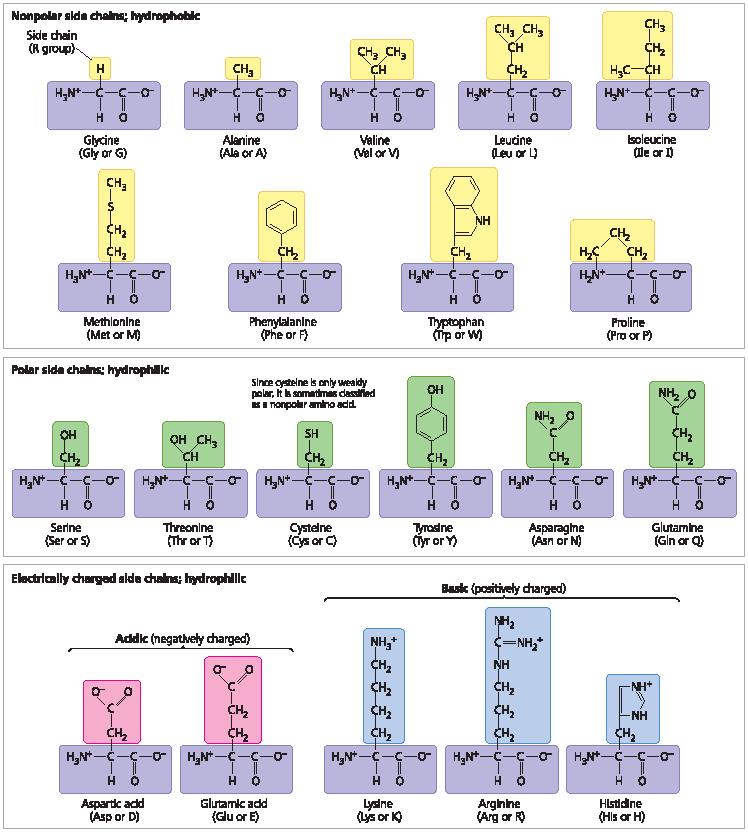
\includegraphics[width=\linewidth]{20种氨基酸.pdf}
	\caption{20种氨基酸}
	\label{fig:20种氨基酸}
\end{figure}

\begin{figure}[htbp]
	\centering
	\includegraphics[width=0.4\linewidth]{Pics/Pyl和Sec}
	\caption{硒代半胱氨酸和吡咯赖氨酸}
	\label{fig:pylsec}
\end{figure}


所有氨基酸都溶于水,只是溶解性不同。

\subsubsection{非蛋白质氨基酸}

非蛋白质氨基酸在合成时不会直接掺入肽链,具体分为下面两种情况:
\begin{enumerate}
	\item 翻译后经化学修饰,如胶原上的羟脯氨酸和羟赖氨酸;
	\item 从不参入蛋白质当中,如神经递质GABA、维生素泛酸的组分$\beta$-丙氨酸、尿素循环中的鸟氨酸、瓜氨酸。
\end{enumerate}

\subsection{氨基酸的性质和功能}

\subsubsection{氨基酸的共同性质}

\paragraph{缩合反应}

即一个氨基酸的氨基和另一个氨基酸的羧基发生缩合反应。

\paragraph{手性}

除了Gly,其他所有氨基酸都至少有一个不对称碳原子(Thr和Ile有两个),即手性碳原子。对于氨基酸手性的判断,在费歇尔投影式中,把羧基放上面、R基放下面,氢原子和氨基一左一右。氨基在左边,则是L-氨基酸;氨基在右边,则是D-氨基酸。

\begin{figure}[htbp]
	\centering
	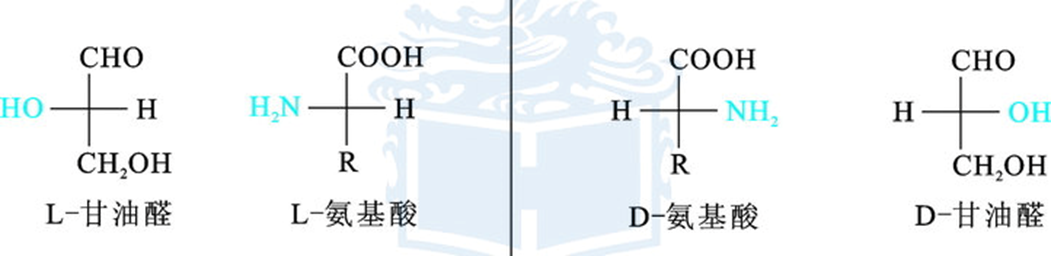
\includegraphics[width=0.8\linewidth]{Pics/L,D-aas}
	\caption{L型、D型氨基酸和甘油醛}
	\label{fig:ld-aas}
\end{figure}


核糖体合成时掺入的氨基酸都是L型。生物合成的蛋白质中,若有D-氨基酸,则一定是合成后异构酶催化的产物,如短杆菌肽、肽聚糖、羊毛硫抗生素、芋螺毒素。

具有手性的分子一般有旋光性,即对偏振光的振动方向产生旋转的特性。一对对映异构体的旋光方向正好相反。氨基酸的L或D型和旋光的方向没有必然联系,具体如何需要通过旋光仪测定。

\begin{gs}[:手性]
	\hspace{2em}在Lewis Carroll的童话世界里,爱丽丝对镜子里的“玻璃奶”充满了好奇,但现实中,这种奶可不好消化。为什么呢?因为生物体内只可以消化和吸收L型蛋白质、D型糖,“玻璃奶”的氨基酸和糖的手性相反,自然不能消化。

	\hspace{2em}制药工程师们现在特别关注药物的“手性”,因为不同的分子形态可能会带来完全不同的效果。比如,1960年欧洲的沙利度胺(thalidomide)事件,这种药物有两种形态,一种能镇静,另一种却会导致婴儿畸形。还有抗组胺药,一种让你昏昏欲睡,另一种则是减充血的好帮手。

	\hspace{2em}有趣的是,我们的味觉和嗅觉也分子的“手性”有关。比如,香芹酮(carvone)的两种构型,一种闻起来像薄荷,另一种则像橙子。柠檬烯(limonene)也是如此,一种闻起来像柠檬,另一种则像橙子。
\end{gs}

\paragraph{特殊酸碱性质与等电点}

氨基酸同时具有酸性的羧基和碱性的氨基,这使得它具有特殊的解离性质。氨基酸的酸性和碱性都弱于单独的胺或羧酸。氨基酸在生理情况下,主要是两性离子:由于其内部的酸碱反应,在一个分子上具有正负两种电荷。

氨基、羧基、有的氨基酸的R基在特定pH下可解离,影响着氨基酸的带电状态。使氨基酸不带电的pH值,称为该氨基酸的等电点。处在等电点的氨基酸,虽然也会少量解离,但解离出阴阳离子的数量相等。

可根据下面方法,在已知各基团的$\mathrm{p}K_{\text{a}}$情况下,计算氨基酸或短肽的等电点:
\begin{enumerate}
	\item 找出所有可解离基团,标注其$\mathrm{p}K_{\text{a}}$;
	\item 假定把该氨基酸(或短肽)放在极低pH下,此时所有基团都质子化;
	\item 逐步提高pH值,$\mathrm{p}K_{\text{a}}$越低的,越先放出质子;
	\item 写出所有可能的解离形式,并找出净电荷为零的那种;
	\item pI即为净电荷为零的情况时,两侧的$\mathrm{p}K_{\text{a}}$相加除以2。
\end{enumerate}

由此,可归纳:
\begin{itemize}
	\item 侧链无可解离基团的氨基酸,pI即两个$\mathrm{p}K_{\text{a}}$除以2;
	\item 酸性氨基酸,pI是两个较低的$\mathrm{p}K_{\text{a}}$除以2;
	\item 碱性氨基酸,pI是两个较高的$\mathrm{p}K_{\text{a}}$除以2.
\end{itemize}

\paragraph{R基团的疏水性}

氨基酸的疏水性直接影响蛋白质的折叠:
\begin{itemize}
	\item 疏水氨基酸一般位于蛋白质内部;
	\item 亲水氨基酸一般位于表面,但是带相反电荷的亲水氨基酸也可以成对出现在蛋白质内部。
\end{itemize}

\paragraph{氨基酸的氨基和羧基参与的化学反应}

\subparagraph{与2,4-二硝基氟苯(DNFB)}

\begin{itemize}
	\item 反应基团:$\alpha$-氨基;
	\item 反应条件:弱碱性;
	\item 产物:黄色的DNP-氨基酸,Pro也可以;
\end{itemize}

肽也可以与DNFB反应,生成DNP-肽。用酸水解后可得到肽链N端氨基酸形成的DNP-氨基酸,再用有机溶剂萃取,可鉴定肽链的N端氨基酸。这叫做蛋白质的Sanger测序。

\subparagraph{与异硫氰酸苯酯(PITC)}

\begin{itemize}
	\item 反应基团:$\alpha$-氨基;
	\item 反应条件:弱碱性;
	\item 产物:PTC-氨基酸$\xrightarrow{\text{酸性}}$PTH-氨基酸,Pro也可以;
\end{itemize}

若是肽与PITC反应,会先生成PTC-肽。之后调节pH至酸性,可释放出N端的PTH-氨基酸。用乙酸乙酯可抽提出PTH-氨基酸。由此,可设计出从N端进行肽链测序的方法,称为Edman降解法。

\subparagraph{与茚三酮}

\begin{itemize}
	\item 反应基团:整个氨基酸;
	\item 反应条件:加热,弱酸性;
	\item 产物:蓝紫色物质(\SI{570}{\nm}处比色),Pro生成黄色物质;
\end{itemize}

该反应非常灵敏,常用于法医采集指纹。

氨基酸与其他物质发生的反应归纳在\autoref{tab:aminoAcidInvolvedReactions}中。

\begin{table}[htbp]
	\zihao{5}
	\centering
	\begin{NiceTabularX}{\textwidth}{>{\centering\arraybackslash}m{4em}>{\centering\arraybackslash}m{9em}>{\centering\arraybackslash}m{9em}X}[hvlines]
		\textbf{反应类型} & \textbf{反应试剂} & \textbf{主要反应产物} & \Block[c]{1-1}{\textbf{用途}} \\
		\Block[v-center]{6-1}{$\alpha$-氨基} & 亚硝酸 & 羟酸、\ce{N2} & Van Slyke 定氮 \\
		& 甲醛 & 二羟甲基氨基酸 & 氨基酸滴定 \\
		& “XX酰氯” & 酰化氨基酸 & \Block[l]{1-1}{人工合肽保护氨基;丹磺酰氯可标记N端氨基酸和定量微量氨基酸} \\
		& DNFB & DNP-氨基酸 & \Block[l]{2-1}{N端氨基酸的鉴定} \\
		& PITC & PTC/PTH氨基酸 &  \\
		& 氨基酸氧化酶、转氨酶等 & 酮酸等 & 细胞内氨基酸的代谢 \\
		\Block[v-center]{2-1}{$\alpha$-羧基} & 碱 & 氨基酸盐 & \Block[l]{2-1}{氨基酸羧基的保护和活化} \\
		& 醇 & 氨基酸酯 &  \\
		\Block[v-center]{4-1}{$\alpha$-氨基和$\alpha$-羧基} & tRNA等 & 氨酰-tRNA & 蛋白质的生物合成 \\
		& 脱羧酶 & 胺 & 氨基酸的代谢 \\
		& 茚三酮 & 紫色物质,Pro为黄色 & 氨基酸的定性和定量 \\
		& 肽酰转移酶等 & 肽 & 多肽和蛋白质的生物合成
	\end{NiceTabularX}
	\caption{氨基酸参与的反应}
	\label{tab:aminoAcidInvolvedReactions}
\end{table}

\subsubsection{个别氨基酸的特殊性质}

\paragraph{F、Y、W的紫外吸收性质}

Phe、Tyr、Trp三种氨基酸的侧链含有苯环,赋予它们近紫外吸收的效应。Trp的紫外吸收最强。Tyr与Trp的吸收峰都靠近\SI{208}{\nm}。

\paragraph{亲水和疏水基团}

疏水基团缺乏反应性,多数时候起到驱动蛋白质折叠的作用,少数蛋白质利用疏水侧链形成口袋结合脂溶性物质。

亲水氨基酸的侧链具有反应性,参与行使多种生物学功能。
\begin{description}
	\item[羟基] S、T、Y三种氨基酸侧链具有羟基,可被磷酸化修饰。
	\item[$\epsilon$-氨基] K具有$\epsilon$-氨基,可作为亲和基团参与酶的催化,与羧基形成酰胺键实现共价连接,与醛基形成席夫碱,发生乙酰化、甲基化、泛酰化修饰。
	\item[巯基和硒醇基] C的巯基可作为亲核基团参与催化。两个巯基可被氧化形成二硫键。U含有还原性更强的硒醇基,具有抗氧化活性。
	\item[咪唑基] H的咪唑基,$\mathrm{p}K_{\text{a}}$约为7,使得它在生理条件下可以作为质子的供体和受体。许多酶的活性中心含有H。咪唑基也可以发生磷酸化修饰。
	\item[羧基] Asp和Glu侧链上含有羧基,在特定情况下可以作为质子的供体和受体,参与广义酸碱催化。羧基带负电荷的特性也可结合金属离子。
\end{description}

\subsection{氨基酸的功能}

\begin{itemize}
	\item 形成肽;
	\item 多种生物活性物质的前体;
	\item 作为神经递质;
	\item 碳骨架氧化分解产生ATP;
	\item 碳骨架作为糖异生或酮体合成的原料。
\end{itemize}

\section{蛋白质的结构}

\subsection{肽}

\subsubsection{肽的分类}
肽即是氨基酸之间发生缩合,形成酰胺键(肽键)产生的聚合物。一般把50个氨基酸残基以上的肽称为蛋白质,因此,具有51个氨基酸残基的胰岛素就是最小的蛋白质。截至\today,最大的蛋白质是PKZILLA-1,来自小定鞭金藻(\textit{Prymnesium parvum})。在此之前,最大的蛋白质被认为是肌巨蛋白。

\subsubsection{肽的理化性质}

\begin{description}
	\item[旋光性] 一种寡肽只要不是全由Gly构成,它就具有旋光性。
	\item[两性解离] 解离基团较少的肽,滴定曲线和单个氨基酸相似。只有小肽才可以使用前述的方法计算pI。
	\item[双缩脲反应] 高中讲过。至少两个肽键(三肽)才可发生此反应。
	\item[水解反应] 肽键可在特定条件水解。
\end{description}

\subsubsection{几种天然活性肽}

活性肽可分为两类:在核糖体上合成的、不在核糖体上合成的。(\autoref{tab:commonBioactivePeptides})
\begin{itemize}
	\item 在核糖体上合成的:只会引入L-氨基酸,形成的肽键总是$\alpha$-氨基与$\alpha$-羧基构成的。通常合成的是前体,经过切割才得到活性肽。
	\item 不在核糖体上合成的:这类肽在不由基因组直接编码,而是通过酶催化合成。它可能含有D-氨基酸,也可能不是严格由是$\alpha$-氨基与$\alpha$-羧基形成肽键(如谷胱甘肽的第一个肽键)。
\end{itemize}

\begin{table}[htbp]
	\centering
	\begin{NiceTabularX}{\textwidth}{>{\centering\arraybackslash}m{5em}cc>{\centering\arraybackslash}m{8em}C}[hvlines]
		类型和种类 & 来源 & 类别 & 功能 & 备注 \\
		\Block{1-5}{非核糖体合成肽} &  &  &  &  \\
		\Block[v-center]{1-1}{谷胱甘肽} & \Block[v-center]{1-1}{动植物细胞} & \Block[v-center]{1-1}{三肽} & \Block[v-center]{1-1}{抗氧化} & 第一个肽键为$\gamma$-肽键 \\
		短杆菌肽 S & 细菌 & 环十肽 & 抗菌 & 含有 D-氨基酸 \\
		肽聚糖中寡肽 & 细菌细胞壁 & 小肽 & 形成细菌细胞壁的网络结构 & 含有 D-氨基酸 \\
		肌肽 & 肌肉细胞 & 二肽 & 不明 & 含有$\beta$-丙氨酸 \\
		\Block{1-5}{核糖体合成多肽} &  &  &  &  \\
		\Block[v-center]{1-1}{TRH} & \Block[v-center]{1-1}{下丘脑} & \Block[v-center]{1-1}{三肽} & \Block[v-center]{1-1}{促甲状腺素释放} & N端焦谷氨酰化,C端酰胺化 \\
		OT & 垂体后叶 & 八肽 & 刺激子宫收缩、排乳、促遗忘 &  \\
		ADH & 垂体后叶 & 八肽 & 升血压、抗利尿、促记忆 &  \\
		$\alpha$-鹅膏蕈碱 & 鬼笔鹅蕈类真菌 & 环八肽 & 真核RNA pol II 强抑制剂 &
	\end{NiceTabularX}
	\caption{常见的生物活性肽}
	\label{tab:commonBioactivePeptides}
\end{table}

\subsection{蛋白质的结构}

蛋白质结构的四个层次是:一级结构、二级结构、三级结构、四级结构。并不是所有蛋白质都含有三级和四级结构。

\subsubsection{蛋白质的一级结构}

蛋白质的一级结构就是氨基酸的排列顺序、二硫键的数目和位置。

肽键具有下面性质:
\begin{description}
	\item[部分双键的性质] 键长介于\ce{C=N}和\ce{C-N}之间。肽键具有的部分双键性质是酰胺N上的孤对电子与相邻羰基C发生共振的结果。
	\item[多为反式(\textit{trans}),也有顺式(\textit{cis})] 核糖体上形成的肽键均为反式。由于空间位阻,反式构象比顺势构象稳定100倍。若出现X-Pro,则由于Pro的四氢吡咯环空间位阻非常大,几乎抵消了反式构象的优势,只比顺式稳定4倍,故此时肽键可以存在顺式构象。蛋白质合成好后,与Pro的亚氨基有关的肽键可被肽基脯氨酰顺反异构酶(PPI)催化变为顺式。
	\item[与肽键有关的6个原子共平面] 该平面称为肽平面或酰胺平面。共面性质是肽键不可旋转带来的。由\autoref{fig:peptidePlane}可见,两个肽平面以C$_{\alpha}$相关,且是两个可自由旋转的单键。规定:\ce{C_{\alpha}-N}旋转形成的为$\phi$角,\ce{C_{\alpha}-C}旋转形成的为$\psi$角。与同一个C$_{\alpha}$相关的$\phi$和$\psi$角称蛋白质的二面角。

	\begin{figure}[htbp]
		\centering
		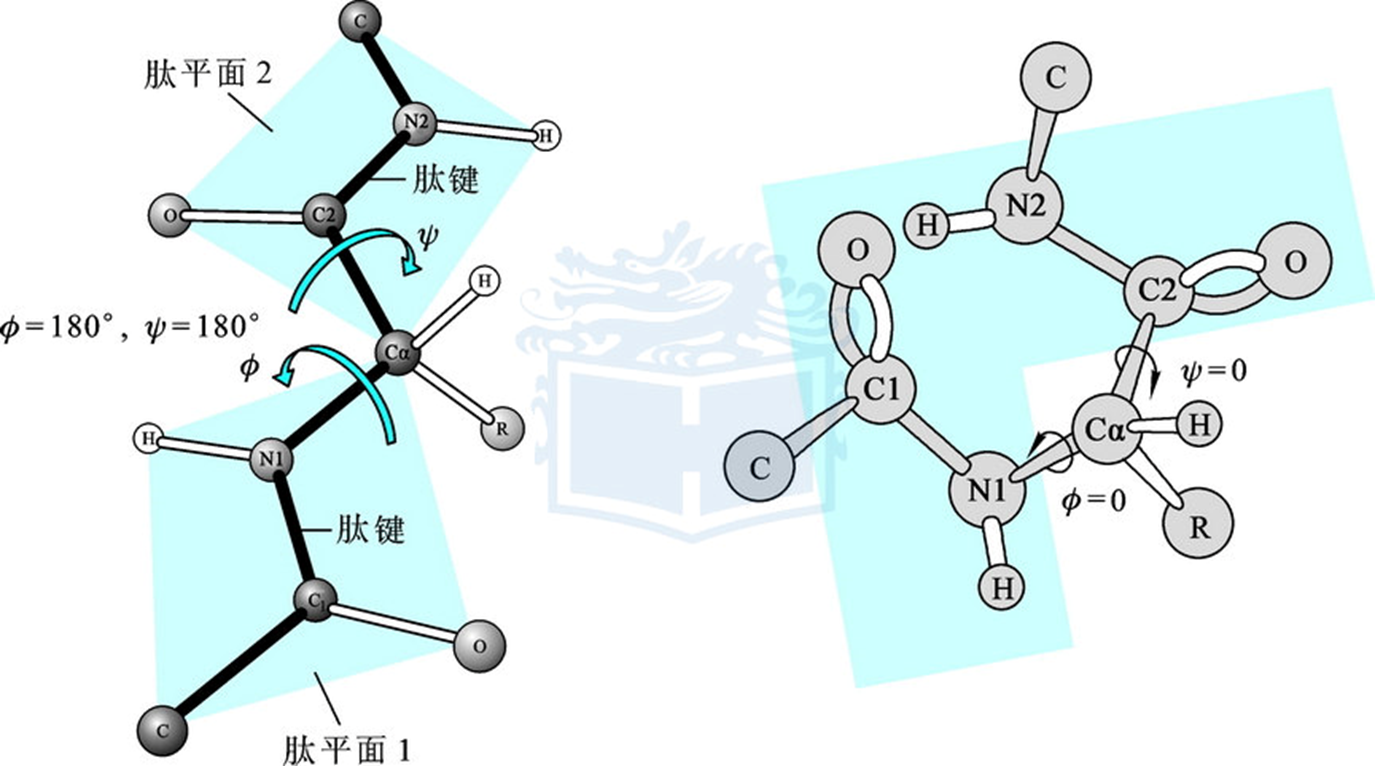
\includegraphics[width=0.8\linewidth]{Pics/肽平面}
		\caption{肽平面和二面角}
		\label{fig:peptidePlane}
	\end{figure}

	二面角的大小是这样规定的:
	\begin{itemize}
		\item 所有肽键共面时,$\psi$和$\phi$角定为$\pm$\SI{180}{\degree};
		\item 若$\psi$的旋转单键\ce{C_{\alpha}-C}两侧的两条化学键呈顺式,则$\psi=0$,$\phi$角同理;
		\item 以\ce{C_{\alpha}}向碳原子和氮原子看,单键顺时针旋转则为正值、逆时针旋转则为负值。
	\end{itemize}

	\begin{qj}[:谁是$\psi$角、谁是$\phi$角?]
		\ce{C_{\alpha}-C}旋转形成的为$\psi$角,可以用$\psi$的形状像横着的C加一竖来联想。
		\ce{C_{\alpha}-N}含氮,“蛋(氮)”是圆的,也就是$\phi$的圆圈。
	\end{qj}

	\begin{tx}[:此二面角非彼二面角]
		这里的二面角和数学立体几何的二面角没有任何关系。此二面角并非两个肽平面的夹角。
	\end{tx}

	在Ramachandran图(\autoref{fig:ramachandran})中,所有可能二面角以坐标$(\phi,\psi)$对应的点表示,形成了图中的有色区域。由于侧链基团的限制,二面角并不能自由变化。

	\begin{figure}[htbp]
		\centering
		\includegraphics[width=0.4\linewidth]{Pics/Ramachandran图}
		\caption{Ramachandran图}
		\label{fig:ramachandran}
	\end{figure}

	\item[部分带电性] 酰胺N带部分正电荷,羰基O带部分负电荷。这是由于二者共振形成的。
\end{description}

\mbox{}

测定蛋白质一级结构的意义:
\begin{itemize}
	\item 有助于理解其三维结构和功能。蛋白质的一级结构包含了决定三维结构的全部信息。
	\item 在分子水平研究生物进化。
\end{itemize}

蛋白质一级结构数据库有:\href{https://cn.expasy.org}{PIR(Protein Information Resource)}、\href{https://www-nbrf.geogetown.edu}{SWISS-PROT}等。
\begin{description}
	\item[PIR] 包含从EMBL翻译来的蛋白质序列,经过检验和注释;
	\item[SWISS-PROT] 包含NCBI从GenBank翻译来的蛋白质序列。
\end{description}

\subsubsection{蛋白质的二级结构}

二级结构指的是肽链主链(不含R基)在局部形成的有规律的折叠和盘绕。二级结构稳定性主要由氢键决定。

常见的二级结构包括:$\alpha$螺旋、三股螺旋、$\beta$折叠、$\beta$转角、$\beta$凸起、无规卷曲和环。按照上述顺序,结构稳定性递减,但功能性递增,因为许多酶的活性中心都是无规卷曲和环构成。

\paragraph{$\alpha$螺旋}

该螺旋的主要特征:
\begin{itemize}
	\item 螺旋的形成是自发的。稳定螺旋的氢键很有规律:若第$n$位的氨基酸残基羰基O为氢键受体,则$n+4$位的氨基酸残基的氨基上H便是氢键供体。(\autoref{fig:hydrogenBondDonorsAndAcceptorsInVariousHelices})

	\begin{figure}[htbp]
		\centering
		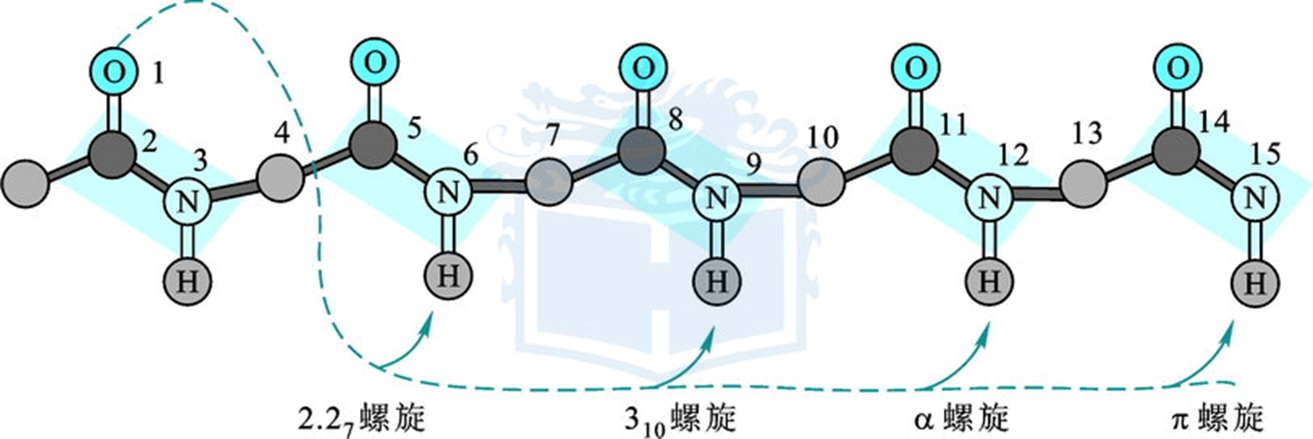
\includegraphics[width=0.8\linewidth]{Pics/各种螺旋的氢键供体与受体}
		\caption{各种螺旋的氢键供体与受体}
		\label{fig:hydrogenBondDonorsAndAcceptorsInVariousHelices}
	\end{figure}

	\item 每个3.6个残基,螺旋上升一圈。一个氨基酸残基环绕螺旋轴\SI{100}{\degree},螺距\SI{0.54}{\nm}。螺旋半径\SI{0.23}{\nm}。
	\item 螺旋方向一般是右手,因为L型氨基酸形成右手螺旋空间位阻小。
	\item 氨基酸残基的R基伸出在螺旋外表面,影响螺旋的形成的带电性。
\end{itemize}

使用多聚氨基酸来研究R基团对$\alpha$螺旋稳定性的影响。
\begin{itemize}
	\item 多聚Leu、多聚Ala容易形成;
	\item 多聚Gly只会形成无规卷曲,多聚Pro只会形成特有的右手螺旋或左手螺旋。
	\item 酸性和碱性氨基酸只有在不带电荷的pH值下才会形成。
\end{itemize}

一般而言,判断一个氨基酸残基是否有利于形成$\alpha$螺旋,要看其R基能否保护主链上的氢键。
\begin{itemize}
	\item Gly不利于形成$\alpha$螺旋,因为侧链太小,二面角变化太大;
	\item Pro通常比较少出现,因为其亚氨基无法作为氢键供体。它只可出现在$\alpha$螺旋的前四个残基中,因为前四个残基不承担氢键供体的角色,如在视紫红质中GPCR;
	\item Ile、Val、Thr、Phe、Trp因为侧链比较大,有较大空间位阻;
	\item Ser、Asp、Asn侧链在靠近主链的位置有氢键供体或受体,可竞争主链的氢键;
	\item 侧链带电荷(没有His),若是同种电荷连续排列,也不利于$\alpha$螺旋形成。
\end{itemize}

偶极矩也是影响$\alpha$螺旋稳定性的因素。螺旋具有一个总偶极矩,正极在N端,负极在C端。螺旋可借助N端的酸性氨基酸和C端的碱性氨基酸来中和偶极矩,或者通过与带电荷的基团或金属离子结合来中和。

用螺旋轮作图可显示出各个氨基酸残基在螺旋边缘的分布情况,有利于判断一个螺旋的亲、疏水性。疏水$\alpha$螺旋经常出现在膜内在蛋白的跨膜区,

\begin{itemize}
	\item 若螺旋上亲水氨基酸较多,则为亲水$\alpha$螺旋;
	\item 若疏水氨基酸较多,则为疏水$\alpha$螺旋,常常出现在膜内在蛋白的跨膜区,如GPCR;
	\item 若二者差不多多,并且亲水氨基酸和疏水氨基酸各分布在螺旋的一侧,则是两亲$\alpha$螺旋,
\end{itemize}

除此$\upalpha$螺旋之外,Pauling还提出了其他螺旋:

\begin{table}[htbp]
	\centering
	\begin{tabularx}{\textwidth}{|c|c|c|C|}
		\hline
		螺旋类型 & 每圈氨基酸残基数 & 氢键环原子数 & 氢键供体位置 \\ \hline
		$2.2_{7}$螺旋 & 2.2 & 7 & $n+2$位残基的氨基H \\ \hline
		$3_{10}$螺旋 & 3 & 10 & $n+3$位残基的氨基H \\ \hline
		$4.4_{16}$螺旋 & 4.4 & 16 & $n+5$位残基的氨基H \\ \hline
	\end{tabularx}
	\caption{其他螺旋}
	\label{tab:many_helix}
\end{table}

在蛋白质中,主要都是$\alpha$螺旋,还没有发现$2.2_{7}$螺旋。

\paragraph{$\beta$折叠}

\paragraph{$\beta$转角}

\paragraph{$\beta$凸起}

\paragraph{无规卷曲与环}

\subsubsection{蛋白质的三级结构}

三级结构可以说就是单条肽链所形成的完整三维结构。三级结构通常由模体和结构域两种超二级结构组成。一种蛋白质的全部三维结构称为构象。

\begin{tx}[:区分“构象”与“构型”]
	构型是指在立体异构中,特定的原子和基团在空间上的几何布局。构型变化必然伴随共价键的断裂和重新形成。构象的转变就只是单键自由旋转造成的。
\end{tx}

\paragraph{稳定三级结构的化学键}

这些化学键主要是次级键,包括:氢键、疏水键、离子键、范德华力。此外,金属配位键、二硫键也发挥一定作用。

\begin{description}
	\item[氢键] 与电负性强的原子相连的氢原子,带部分正电荷,可作氢键供体;一些电负性较强,带部分负电荷的原子则作为氢键受体。在三级结构中,氢键的供体、受体主要来源于氨基酸侧链基团,而不是二级结构里,来自主链。
	\item[离子键] 即静电作用。又称为盐键、盐桥。离子键的形成主要依赖于带电荷的氨基酸侧链基团和肽链首尾游离的氨基、羧基。
	\item[疏水键] 疏水基团或疏水分子在水溶液里为了避开水相互聚集的作用力就是疏水键(疏水作用力)。主要由疏水氨基酸残基提供。疏水氨基酸会在蛋白质内部形成疏水核心。疏水键是稳定三级结构最重要的作用。
	\item[范德华力]
	\item[配位键] 配位键对某些金属蛋白的稳定起作用。
	\item[二硫键] 含有二硫键的蛋白质一般是分泌蛋白或膜蛋白,胞内蛋白很少有二硫键。但是古菌很多胞内蛋白质也具有二硫键。
\end{description}

\paragraph{三级结构的部件}

\subparagraph{模体}

模体的概念有两个,一个指的是一级结构,即氨基酸的特定序列(序列模体)。另一个介于三级结构和二级结构之间,即结构模体。

结构模体是由相邻的二级结构单位的疏水氨基酸残基相互作用,形成的二级结构组合体。

常见的模体有:

%\begin{table}[]
%	\centering
%	\begin{tabularx}{\textwidth}{|c|m{10em}|l|X|}
%		\hline
%		\textbf{模体} & \multicolumn{1}{c|}{\textbf{结构特点}} & \multicolumn{1}{c|}{\textbf{功能}} & \multicolumn{1}{c|}{\textbf{存在}} \\ \hline
%		卷曲螺旋 & 多股$\alpha$螺旋聚合体形成左手超螺旋,螺旋之间平行或反平行,含七肽重复序列 & 蛋白质折叠、相互作用 & SNARE \\ \hline
%		HLH & 两个螺旋、中间一个环 & 环用来结合\ce{Ca^{2+}},碱性HLH这类模体可结合DNA大沟 & 传感器蛋白、转录因子 \\ \hline
%		$\beta$-$\alpha$-$\beta$ & 平行的$\beta$折叠、$\alpha$螺旋 &  &  \\ \hline
%		$\beta$发夹环 & 两股反平行$\beta$股和一段连接小环 &  &  \\ \hline
%		HTH & 如图 & 一个alpha螺旋以亲水氨基酸残基结合DNA & 与DNA特异结合的蛋白质 \\ \hline
%		Rossmann折叠 & 形成$\beta$  含有疏水核心 &  & 需要辅酶I或辅酶II的酶 \\ \hline
%		希腊钥匙 & 全$\beta$折叠聚合体 &  & 清蛋白原、质体蓝素 \\ \hline
%		$\beta$螺旋 & 多个$\beta$股,右手或左手 & 促进蛋白质相互作用 & 果胶酸裂合酶(右手) \\ \hline
%	\end{tabularx}
%	\caption{蛋白质结构模体}
%	\label{tab:structure_motif}
%\end{table}

\subparagraph{结构域}

较大的蛋白质一般会折叠成多个相互独立的球状区域,即结构域。疏水核心是结构域稳定存在必需的。结构域有大有小,但不会太大。大的结构域疏水核心较大,更稳定;小的结构域疏水核心较小,不稳定,需要靠金属离子或二硫键加固。

结构域在结构和功能上都是独立的。许多蛋白质的结构域被人为分开后,依然能保持活性。

\subsubsection{蛋白质的四级结构}


\subsection{蛋白质的折叠历程}

\section{蛋白质结构和功能之间的关系}

\subsection{蛋白质的功能}

\subsection{蛋白质结构和功能之间的关系}

\subsection{几种重要的蛋白质和功能}

\subsubsection{纤维状蛋白质}

\paragraph{$\alpha$角蛋白}

\paragraph{$\beta$角蛋白}

\paragraph{胶原蛋白}

\subsubsection{球状蛋白——珠蛋白}

\subsubsection{球状蛋白——免疫球蛋白}

\subsubsection{膜蛋白}

\subsubsection{天然无折叠蛋白}


\section{核苷酸}

\subsection{核苷酸的结构与组成}

$\text{核苷酸}=\text{核苷}+\text{磷酸基团}=\text{D-核糖或D-脱氧核糖}+\text{碱基}+\text{磷酸基团}$,碱基和戊糖之间通过$\beta$-N-糖苷键连接。

\subsubsection{碱基}

碱基即含氮碱基,包括嘌呤和嘧啶。它们的结构及原子编号见\autoref{fig:puring_pyrding}。

嘧啶为六元芳香杂环,平面结构;嘌呤由六元的嘧啶环和五元的咪唑环融合而成,实验表明两个环之间成一定角度,尽管理论上应当是平面结构。

常见的碱基有腺嘌呤(A)、鸟嘌呤(G)、胞嘧啶(C)、胸腺嘧啶(T)、尿嘧啶(U)五种。RNA与DNA共有的是A、G、C,而U通常只存在于RNA,T通常只存在于DNA,不过也有例外。如tRNA上的T$\upPsi$C环中含有T碱基,有时DNA上会出现U。
\begin{figure}
	\centering
	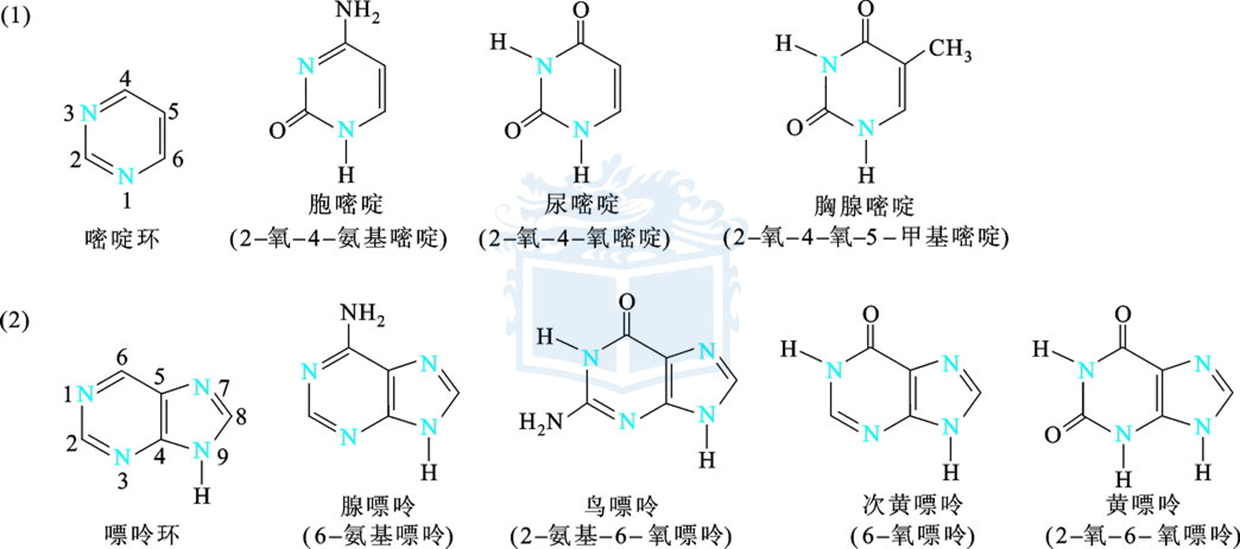
\includegraphics[width=\linewidth]{Pics/嘧啶环和嘌呤环的编号以及各种碱基的化学结构}
	\caption{嘧啶环和嘌呤环的编号以及各种碱基的化学结构}
	\label{fig:puring_pyrding}
\end{figure}


机体的修饰碱基有:5-甲基胞嘧啶(m$^{5}$C)、N$^{6}$-甲基腺嘌呤(m$^{6}$A)、黄嘌呤(X)、次黄嘌呤(I)等。m$^{5}$C和m$^{6}$A具有表观遗传功能,可抑制所在基因的表达,其中线虫、果蝇基因组中含有的是m$^{6}$A。

茶碱和咖啡因是腺苷(A)的类似物,可以与肌细胞和脑细胞膜上的腺苷受体结合,提高心率和产生兴奋,这便是喝茶或咖啡提神的原理;还可以在胞内充当催化cAMP水解的磷酸二酯酶的抑制剂,加强依赖cAMP通路的激素的作用效果。

碱基具有以下化学性质:
\begin{description}
	\item[紫外吸收] 碱基的共轭双键赋予其紫外吸收性质,最大吸收值在\SI{260}{\nano\meter}。
	\item[可发生互变异构] 嘧啶碱基:酮式$\rightleftharpoons$烯醇式,腺嘌呤:氨基式$\rightleftharpoons$亚氨基式。这两种互变异构体在体内都以前者为极多,但是碱性条件下可向后者移动。碱基互补配对规则只适用于酮式和氨基式的碱基。(\autoref{fig:base_change})

	\begin{figure}[htbp]
		\centering
		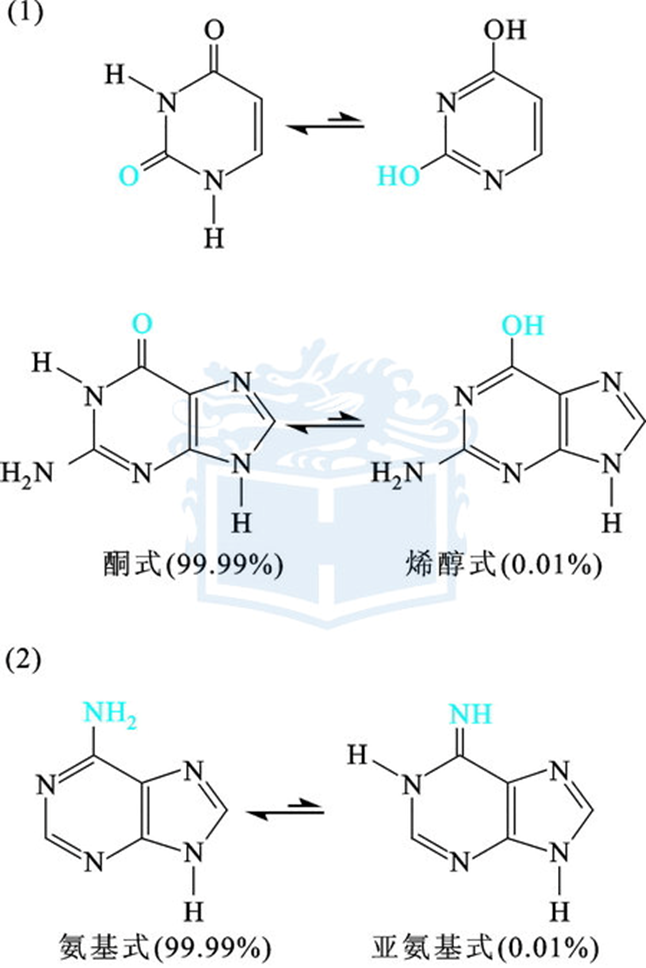
\includegraphics[width=0.5\linewidth]{Pics/碱基互变异构}
		\caption{碱基互变异构}
		\label{fig:base_change}
	\end{figure}

	\item[水溶性差] 这是由碱基的芳香杂环决定的。因此能形成稳定的DNA双螺旋结构。
	\item[解离] pH决定了环上各个N原子是否与\ce{H+}结合,影响氢键的供受体关系、碱基配对规则。中性条件下,碱基主要以内酰胺形式存在。
\end{description}

\subsubsection{核苷}

核苷是碱基和核糖通过$\beta$-N-糖苷键形成的糖苷。该糖苷键由核糖的异头C与嘧啶碱基的N1或嘌呤碱基的N9形成。(\autoref{fig:structure_nucleoside})

\begin{figure}[htbp]
	\centering
	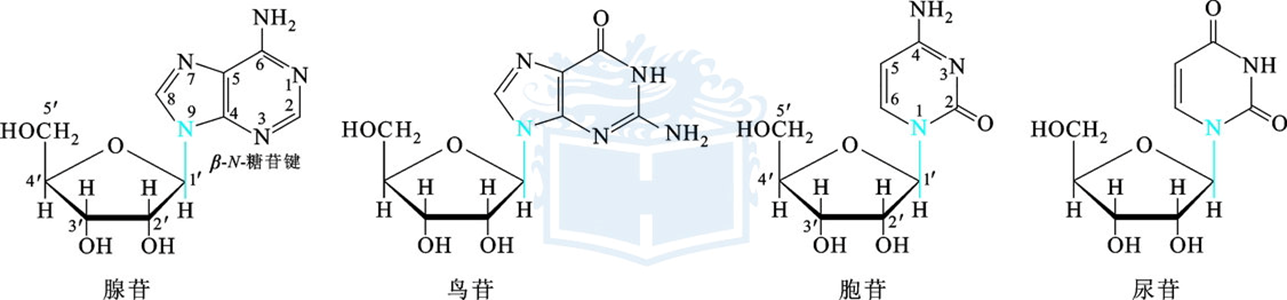
\includegraphics[width=\linewidth]{Pics/核苷的结构}
	\caption{核苷的结构}
	\label{fig:structure_nucleoside}
\end{figure}

生物体内核苷的糖苷键都是$\beta$-N-糖苷键,$\beta$的意思是碱基在核糖环上方。生物体内的核苷没有$\alpha$-N-糖苷键。

嘧啶核苷只有反式构象,嘌呤核苷多数是反式构象,仅在Z-DNA中是顺式。(\autoref{fig:syn_anti_nucleoside})

\begin{figure}[htbp]
	\centering
	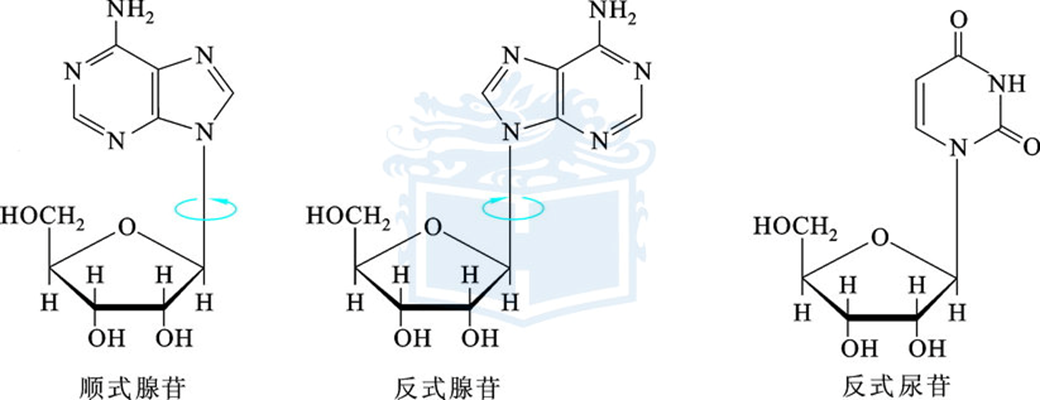
\includegraphics[width=0.7\linewidth]{Pics/核苷的构象}
	\caption{核苷的构象}
	\label{fig:syn_anti_nucleoside}
\end{figure}

常见的核苷如\autoref{fig:structure_nucleoside}所示。它们的核糖变为脱氧核糖,就是脱氧核苷。

修饰核苷是指碱基有修饰的、或核糖有修饰的、或以特殊成键方式存在的核苷。例如假尿苷($\upPsi$),是以C5与核糖相连。(\autoref{fig:modified_nucleoside})

\begin{figure}[htbp]
	\centering
	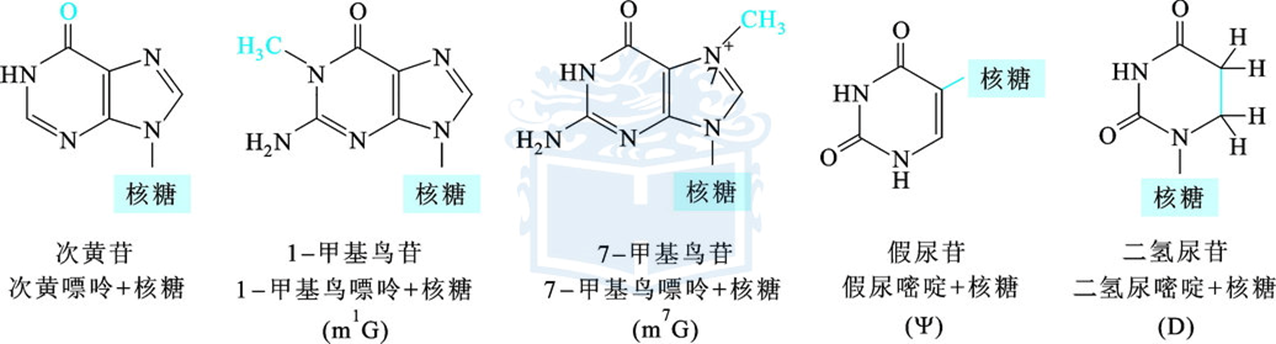
\includegraphics[width=\linewidth]{Pics/几种修饰核苷}
	\caption{几种修饰核苷}
	\label{fig:modified_nucleoside}
\end{figure}

核苷的性质如下:

\begin{description}
	\item[水溶性] 因为核糖亲水,所以核苷的水溶性比单独的碱基高。
	\item[水解] 只有嘌呤核苷容易被酸水解,意思是:所有核苷可抵抗碱水解、嘧啶核苷还可抵抗酸水解。
\end{description}

\subsubsection{核苷酸}

自然界的核苷酸多为核苷-5′-磷酸。(\autoref{fig:structuresOfCommonNucleotides})

\begin{figure}[htbp]
	\centering
	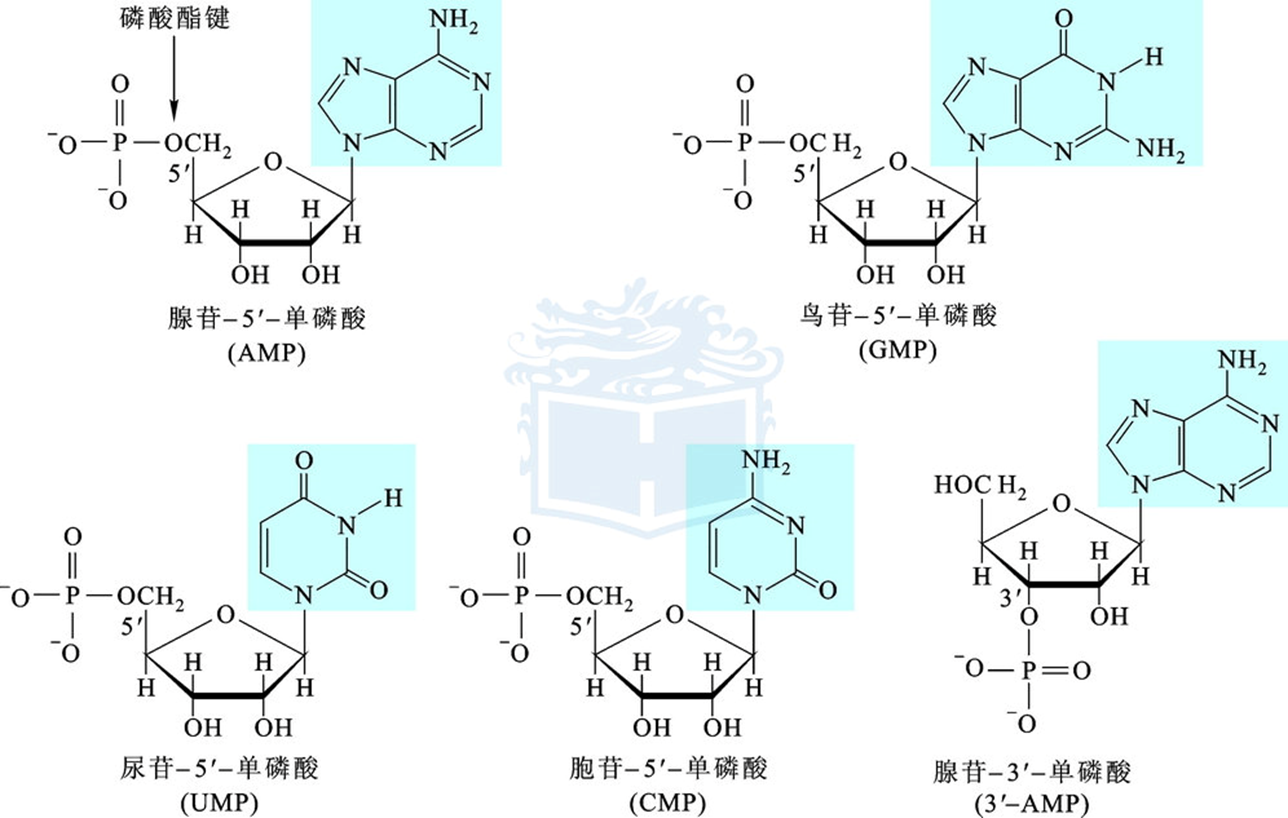
\includegraphics[width=0.9\linewidth]{Pics/常见核苷酸的结构}
	\caption{常见核苷酸的结构}
	\label{fig:structuresOfCommonNucleotides}
\end{figure}

核苷酸的磷酸基团还可以增加到3个。这三个磷酸基团从最靠近核糖的那个开始,依次称为$\alpha$、$\beta$、$\gamma$磷酸。

某些核苷三磷酸可形成环核苷酸,作为第二信使。

核苷酸的构象不是固定不变的,而是具有一定柔性。

核苷酸的理化性质由组成它的核糖、碱基等决定。

\section{核酸的结构与功能}

\subsection{核酸的分类}

核酸分为核糖核酸(RNA)和脱氧核糖核酸(DNA),二者直接的区别就是构成它们的戊糖,在2′位的是羟基还是氢原子。

因为RNA有2′-OH,所以理论上可以形成2′-5′磷酸二酯键。只有在高等动物体内干扰素在作用时才诱导靶细胞合成以2′-5′磷酸二酯键相连接的多聚A。

DNA和RNA的差别列在\autoref{tab:DNA_RNA}中:

\begin{table}[htbp]
	\centering
	\begin{tabularx}{\textwidth}{|c|C|C|}
		\hline
		\textbf{性质} & \textbf{RNA} & \textbf{DNA} \\ \hline
		戊糖 & D-核糖 & 2′-D-脱氧核糖 \\ \hline
		碱基 & 第四个碱基通常是U & 第四个碱基通常是T \\ \hline
		多聚核苷酸链的数目 & 多为单链 & 多为双链 \\ \hline
		在细胞内的双螺旋 & A型 & B型和Z型 \\ \hline
		种类 & 多种 & 只有一种 \\ \hline
		功能 & 功能多样 & 仅充当遗传物质 \\ \hline
		碱溶液下的稳定性 & 不稳定,很容易水解 & 稳定 \\ \hline
	\end{tabularx}
	\caption{DNA和RNA的比较}
	\label{tab:DNA_RNA}
\end{table}

DNA和RNA主要有三点差别:
\begin{description}
	\item[戊糖:RNA是核糖,DNA是脱氧核糖] 这是判断核酸是DNA还是RNA的唯一标准。RNA的2′-OH是具有反应性的亲核基团,使之容易碱水解。不易降解的RNA,如rRNA和tRNA,其上很多2′-OH都被甲基化,失去反应性。
	\item[碱基:RNA是U,DNA是T] DNA上正常无U,相当于是标记上突变的碱基,便于修复。这项差别并不绝对。RNA中可能出现的T来自于U甲基化,DNA中的U来自于dUTP的错误掺入或C自发脱氨基。DNA天然含U的情形:
	\begin{itemize}
		\item 枯草杆菌PBS2噬菌体完全用U取代了基因组里的T;
		\item 昆虫化蛹时,调控酶的活性,掺入大量U进入DNA,作为细胞死亡的信号。
	\end{itemize}
	\item[单双链:RNA单链,DNA双链]DNA双链更稳定,RNA单链变化更多。但也不绝对。如一些病毒具有单链DNA或双链RNA。miRNA也是双链RNA。
\end{description}

生物体内有多种天然小RNA,功能多样。

\mbox{}

核酸具有一级结构、二级结构、三级结构,但没有四级结构。

\subsection{核酸的一级结构}

核酸的一级结构就是核苷酸或碱基的排列顺序。

核酸具有极性,单链的一头有游离的3′-OH,另一头有游离的5′-OH。

除了线型核酸外,在细菌、质粒、叶绿体、大多数线粒体DNA都是环形的。它们完全没有游离的3′-OH或5′-OH。

\subsection{核酸的二级结构}

\subsubsection{DNA的二级结构}

DNA的二级结构主要就是各种螺旋。DNA的双螺旋结构是由Waston和Crick在1953年4月25日发表在\textit{Nature}上的。(\autoref{fig:discover_DNA_double_helix})

\begin{figure}[htbp]
	\centering
	\begin{subfigure}{0.3\textwidth}
		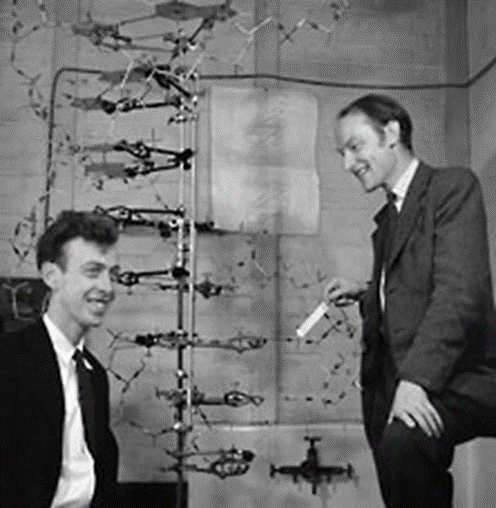
\includegraphics[width=\linewidth]{W&C,DNA双螺旋1}
		\caption{Waston和Crick发现了DNA双螺旋结构}
	\end{subfigure}
	\hfill
	\begin{subfigure}{0.3\textwidth}
		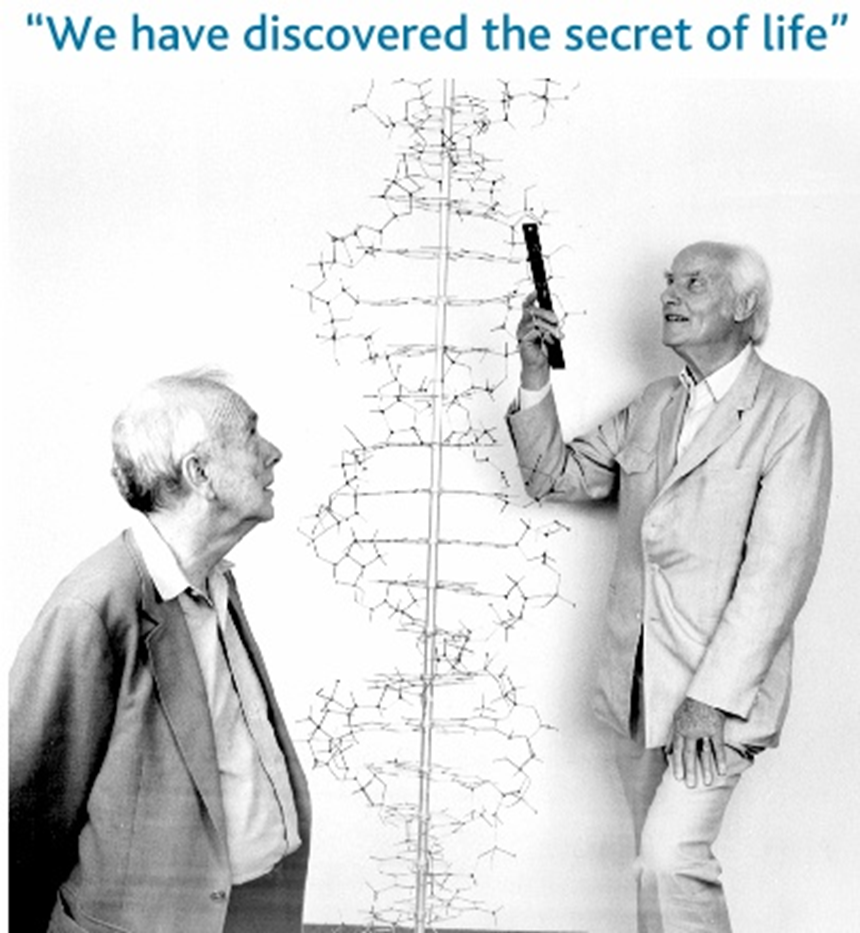
\includegraphics[width=\linewidth]{W&C,DNA双螺旋2}
		\caption{已步入古稀之年的Watson(左)和Crick(右)在讨论DNA双螺旋结构模型}
	\end{subfigure}
	\hfill
	\begin{subfigure}{0.3\textwidth}
		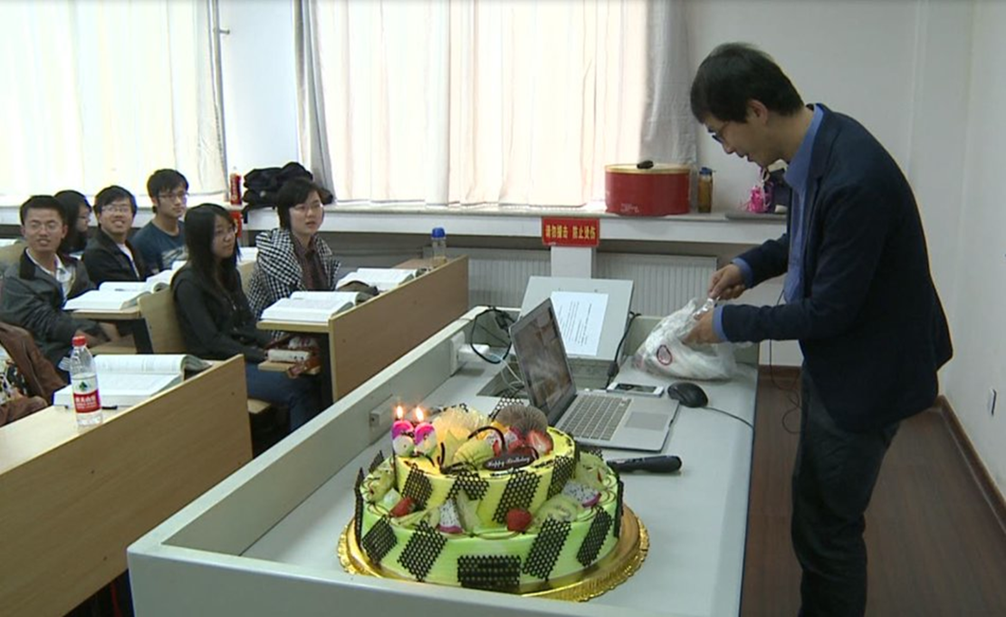
\includegraphics[width=\linewidth]{R.Young,DNA双螺旋3}
		\caption{2013年4月25日,杨荣武教授为DNA双螺旋结构庆生}
	\end{subfigure}
	\caption{DNA双螺旋结构的发现}
	\label{fig:discover_DNA_double_helix}
\end{figure}

A、B、Z螺旋的特征概括如


\paragraph{支持DNA双螺旋结构的证据}

\paragraph{DNA的非标准二级结构}

DNA可形成弯曲、十字形、三螺旋、滑移错配DNA、碱基翻转这些非标准二级结构。

形成这些结构的原因可能是受到蛋白质作用,或是DNA拥有独特的序列模体:反向重复、回文序列、镜像重复、直接重复、高嘌呤序列、高嘧啶序列(\autoref{fig:dna_specific_sequence_motif})、富含A序列、富含G序列等。

\begin{figure}[htbp]
	\centering
	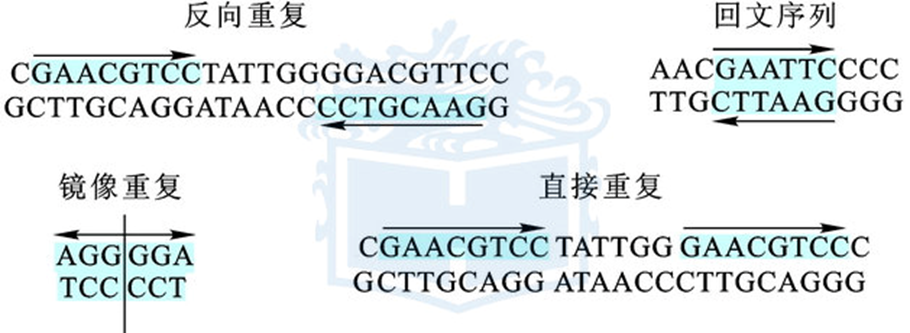
\includegraphics[width=0.7\linewidth]{Pics/DNA的特殊序列模体}
	\caption{DNA的特殊序列模体}
	\label{fig:dna_specific_sequence_motif}
\end{figure}

\begin{figure}[htbp]
	\centering
	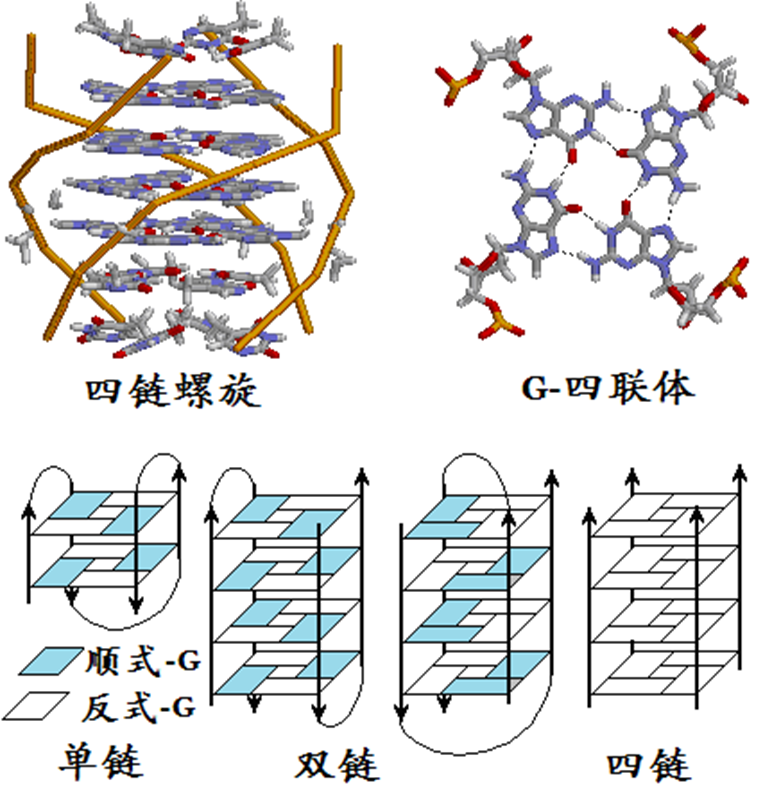
\includegraphics[width=0.5\linewidth]{Pics/DNA的四链结构}
	\caption{DNA的四链结构}
	\label{fig:dna_4strand}
\end{figure}


\subparagraph{弯曲}
\subsubsection{RNA的二级结构}

RNA有很丰富的二级结构。(\autoref{fig:rna_second_structure})自然界的RNA多数都是单链,但依然可以通过自我折叠形成局部的A型双螺旋。

\begin{figure}[htbp]
	\centering
	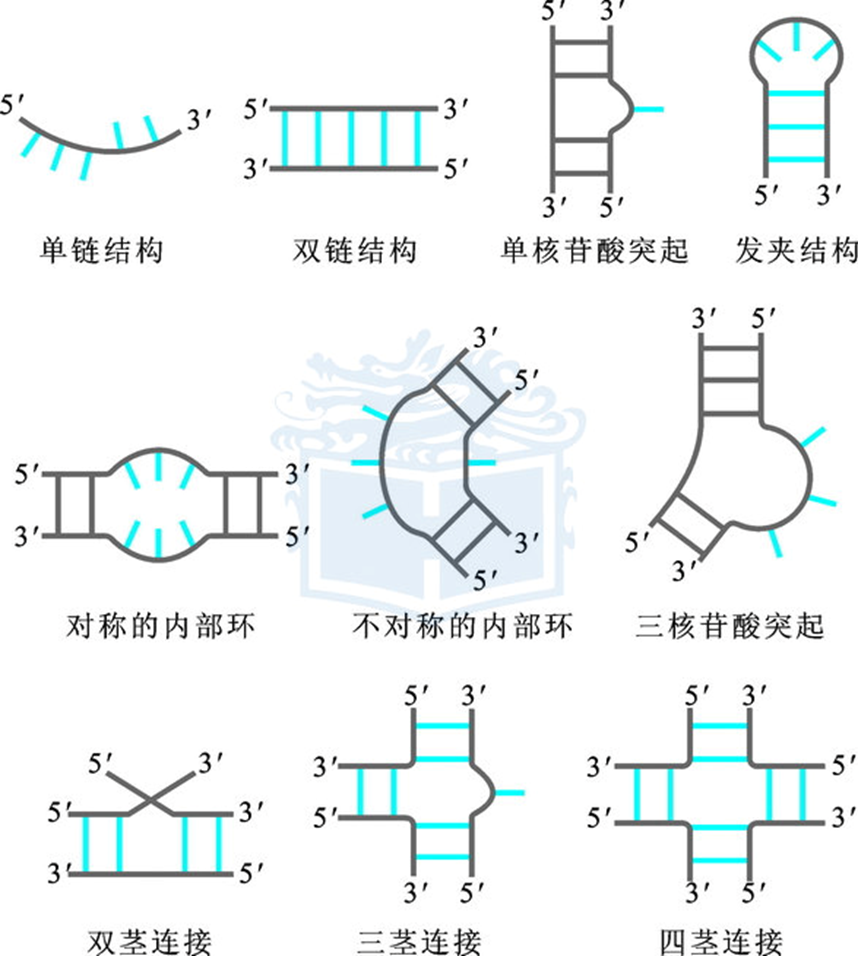
\includegraphics[width=0.7\linewidth]{Pics/RNA的二级结构}
	\caption{RNA的二级结构}
	\label{fig:rna_second_structure}
\end{figure}


\section{核酸的理化性质}

\subsubsection{紫外吸收}

\subsubsection{酸碱解离}

\subsubsection{黏度}

\subsubsection{沉淀}

\subsubsection{变性}

核酸变性不涉及任何共价键断裂,只是二级结构、三级结构的改变。

\section{酶学概论}

\subsection{酶的化学本质}

大多数酶都是蛋白质,少数酶是RNA。这种具有催化活性的RNA称为\sy{核酶}。

酶可按化学组成分类:(\autoref{fig:class_enzyme})

\begin{figure}[htbp]
	\centering
	\begin{forest}
		forest scheme
		[酶
			[单纯酶]
			[缀合酶
				[多肽链]
				[非氨基酸的辅因子
					[辅酶:结合松散,如辅酶I、辅酶II]
					[辅基:结合紧密,如FAD]
					[金属离子]]]]
	\end{forest}
	\caption{酶按化学组成的分类}
	\label{fig:class_enzyme}
\end{figure}

丧失辅因子的酶成为脱辅酶,结合了辅因子的酶称全酶。含紧密结合的金属离子的酶通常称为金属酶。

大多数核酶都含有金属离子和(或)蛋白质,仅有少数是单独的RNA。

\subsection{酶的催化性质}

酶的催化性质有:
\begin{enumerate}
	\item 高效性;
	\item 酶在活性中心与底物结合;
	\item 高度专一性;
	\item 反应条件温和;
	\item 对反应条件敏感,易失活;
	\item 受到调控;
	\item 许多酶的活性需要辅因子存在。
\end{enumerate}

下面对上述部分名词作解释。

\subsubsection{活性中心}

活性中心是酶与底物结合,直接参与催化的部位。缀合酶的活性中心还包括和底物结合的部分。多功能酶有多个活性中心。

活性中心由结合基团和催化基团构成,前者决定专一性,后者决定催化能力。但有些基团可能同时承担二者功能。

活性中心的一般特征:
\begin{description}
	\item[是三维实体,相关氨基酸残基一级结构不相邻。] 活性中心的三维实体结构是蛋白质正确折叠后的必然产物。
	\item[所占体积小] 酶上的大多数氨基酸残基并不与底物接触,起到稳定活性中心的作用。
	\item[呈裂隙、口袋状] 活性中心内部多为疏水氨基酸残基,也有少量亲水的。
	\item[只有亲水氨基酸残基可催化反应] 疏水氨基酸侧链是惰性的,无法催化反应。活性中心中出现的亲水氨基酸频次:H>C>D>R>E。
	\item[大多靠多重次级键与底物结合] 在共价催化中,酶与底物形成暂时的共价键。
	\item[结构互补性] 活性中心与底物过渡态的互补性优于底物。
	\item[具有柔性] 构象会发生改变。
\end{description}

\subsubsection{专一性}

专一性的类型:
\begin{description}
	\item[绝对专一性] 酶仅严格催化一个反应。
	\item[相对专一性] 这是大多数酶的专一性类型。包括基团专一性和键专一性。这就是说酶只作用于特定的基团或化学键。
	\item[立体专一性] 酶对具有立体异构体的底物,只作用于其中一种。进一步分为旋光异构专一性和几何异构专一性。前者即底物的D、L型,后者即底物的顺、反式。
\end{description}

酶的立体专一性还表现在能区分假手性C上两个我们看似相同的基团。例如:
\begin{itemize}
	\item 一端由\ce{C^{14}}标记的甘油,由甘油激酶催化加磷酸,只生成1-磷酸甘油。(\autoref{fig:stereospec_glycerolkinase})

	\begin{figure}[htbp]
		\centering
		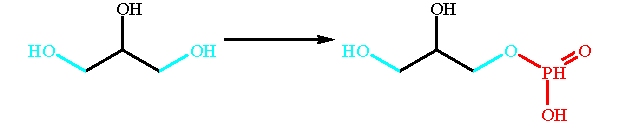
\includegraphics{甘油激酶的立体专一性}
		\caption{甘油激酶的立体专一性}
		\label{fig:stereospec_glycerolkinase}
	\end{figure}

	\item 顺乌头酸酶只会把羟基给来自草酰乙酸的\ce{-CH2-COOH},而不会给来自乙酰CoA的。(\autoref{fig:FumaraseStereoSpecificity})

	\begin{figure}[htbp]
		\centering
		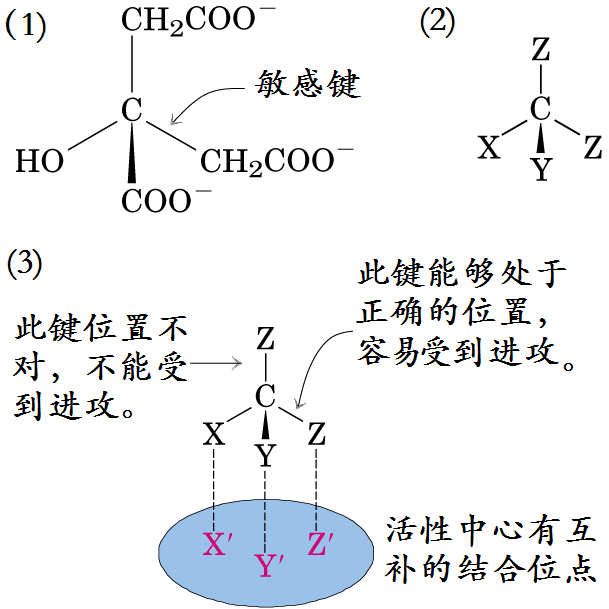
\includegraphics[width=0.3\linewidth]{Pics/顺乌头酸酶的立体专一性}
		\caption{顺乌头酸酶的立体专一性}
		\label{fig:FumaraseStereoSpecificity}
	\end{figure}

	\item 酵母乙醇脱氢酶(YADH)在催化时,辅酶NADH上的烟酰胺环,只有一侧是可以加氢或脱氢的。(\autoref{fig:yadh})

	\begin{figure}[htbp]
		\centering
		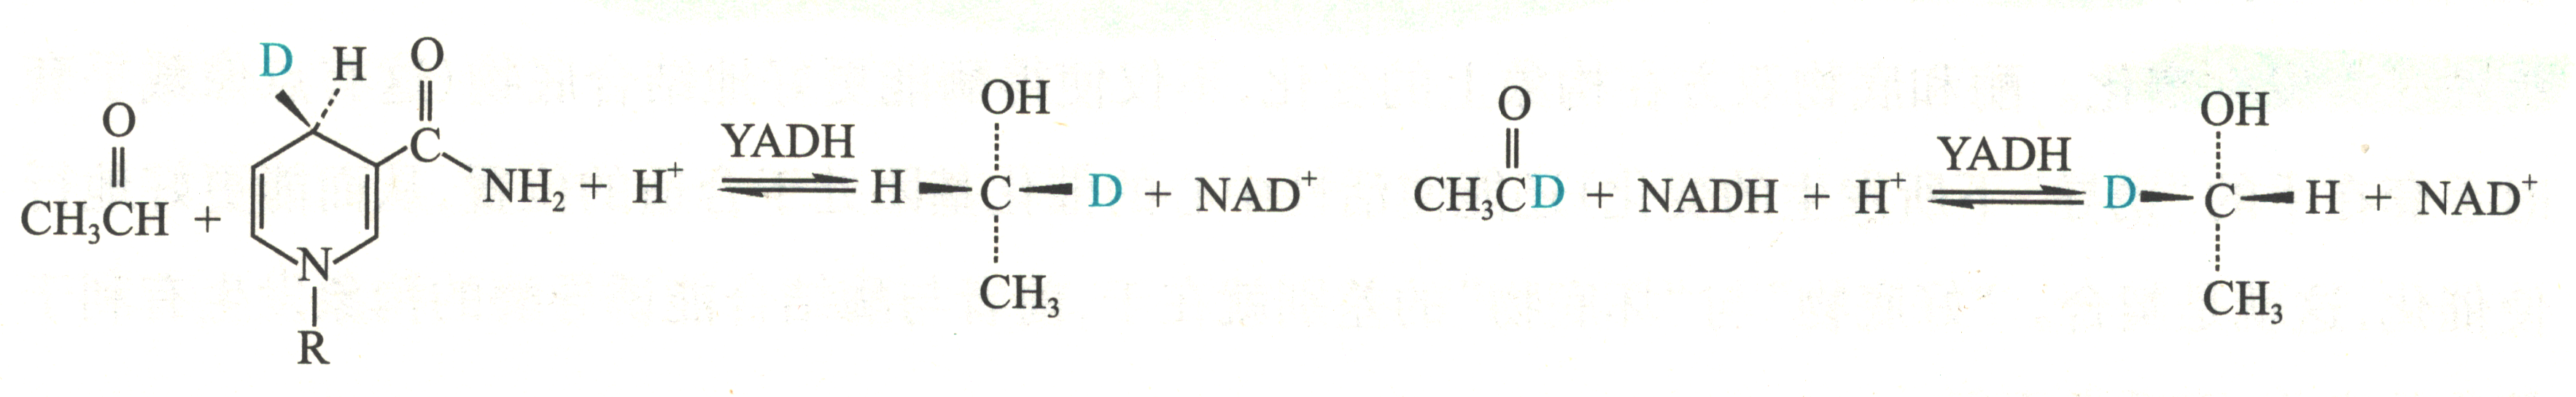
\includegraphics{YADH的立体专一性}
		\caption{YADH的立体专一性}
		\label{fig:yadh}
	\end{figure}

\end{itemize}

YADH这种专一性定为A型,有相同专一性的脱氢酶被称为A型脱氢酶,如苹果酸脱氢酶、异柠檬酸脱氢酶、乳酸脱氢酶。不具有这种专一性的酶称为B型酶,如谷氨酸脱氢酶、3-磷酸甘油脱氢酶。

有三个作用可解释酶的立体专一性:
\begin{description}
	\item[“锁与钥匙”模型] 比较过时,早已被淘汰。
	\item[“诱导契合”模型] 酶活性中心是柔性可变的。一开始酶和底物并不契合,当二者靠近,酶活性中心和底物的构象都发生变化(诱导),使活性中心更好结合底物(契合)。
	\item[“三点附着”模型] 底物在活性中心有3个结合位点,只有当3个结合位点都匹配,才会催化反应。这可以解释立体专一性。
\end{description}

\subsection{酶的分类}

根据反应的性质,把酶分为七类:(\autoref{tab:酶的分类})

\begin{table}[htbp]
	\zihao{5}
	\centering
	\begin{tabularx}{\textwidth}{|cCc|}
		\hline
		\multicolumn{1}{|c|}{类别} & \multicolumn{1}{c|}{反应性质} & 实例 \\ \hline
		\multicolumn{1}{|c|}{氧化还原酶} & \multicolumn{1}{c|}{电子转移} & 乙醇脱氢酶 \\ \hline
		\multicolumn{3}{|l|}{包括:脱氢酶,氧化酶,还原酶,过氧化物酶,过氧化氢酶,加氧酶,羟化酶} \\ \hline
		\multicolumn{1}{|c|}{转移酶} & \multicolumn{1}{c|}{分子间基团转移} & 蛋白激酶 A \\ \hline
		\multicolumn{3}{|l|}{包括:转醛酶和转酮酶,脂酰基、甲基、糖基和磷酸基转移酶,激酶,磷酸变位酶} \\ \hline
		\multicolumn{1}{|c|}{水解酶} & \multicolumn{1}{c|}{通过加水导致键的断裂} & 脂肪酶 \\ \hline
		\multicolumn{3}{|l|}{包括:酯酶,糖苷酶,肽酶,磷酸酶,硫酯酶,磷脂酶,酰胺酶,脱氨酶和核酸酶} \\ \hline
		\multicolumn{1}{|c|}{裂合酶} & \multicolumn{1}{c|}{消除反应,产生双键} & 碳酸酐酶 \\ \hline
		\multicolumn{3}{|l|}{包括:脱羧酶,醛缩酶,水合酶,脱水合酶,合酶,裂解酶} \\ \hline
		\multicolumn{1}{|c|}{异构酶} & \multicolumn{1}{c|}{分子内的重排} & TIM \\ \hline
		\multicolumn{3}{|l|}{包括:消旋酶,差向异构酶,异构酶,变位酶} \\ \hline
		\multicolumn{1}{|c|}{连接酶} & \multicolumn{1}{c|}{水解 ATP 与分子之间的连接偶联} & DNA 连接酶 \\ \hline
		\multicolumn{3}{|l|}{包括:合成酶和羧化酶} \\ \hline
		\multicolumn{1}{|c|}{转位酶} & \multicolumn{1}{c|}{与NTP水解或氧化还原酶反应偶联的物质跨膜转运或在膜内的分离} &  \\ \hline
		\multicolumn{3}{|l|}{包括:F型质子泵、ABC超家族等} \\ \hline
	\end{tabularx}
	\caption{酶的分类}
	\label{tab:酶的分类}
\end{table}

\begin{tx}[:区分合酶和合成酶]

	合酶催化的反应是缩合反应,但并没有与ATP的水解相偶联,而合成酶属于第六类酶,所催化的反应一定与ATP或者它的等价物的降解相偶联。
\end{tx}

\begin{qj}[:七大类酶]
	想要记住七大类酶的名称和顺序,记住前六类分别是:养(氧化还原酶)鱼(转移酶)水(水解酶)活(裂合酶)鱼(异构酶)活(合成酶),再加上第七类转位酶即可。
\end{qj}



\section{酶动力学}

\subsection{影响酶促反应速率的因素}

\subsubsection{外因}

\paragraph{温度}

温度对酶促反应速率的关系图象呈倒V型,最大值处为酶的最适温度。温度系数(即范特霍夫系数)Q$_{10}$表示温度每上升\SI{10}{\celsius},反应速率加快的倍数。

偏离最适温度,高温使酶变性,低温不变性,但活性也降低。

酶的最适温度不是酶的特征性常数,还与反应持续时间有关。如有的酶只能短时间耐受高温。

\paragraph{pH}



\subsubsection{内因}

内因就是酶浓度和底物浓度。

\begin{description}
	\item[酶浓度] 底物过量时,反应速率与酶浓度成正比。
	\item[底物浓度] 酶的浓度一定时,反应速率与底物的关系呈双曲线或S型,且具有饱和动力学特征(存在最大速率)。这一饱和动力学特征可用“酶-底物中间物”假说来解释:
	\begin{center}
		E+S$\longrightarrow$ES$\longrightarrow$EP$\longrightarrow$E+P
	\end{center}
\end{description}

\subsection{米氏动力学}

\subsubsection{米氏方程}

米氏方程基于下面三个条件:
\begin{itemize}
	\item 反应速率为初速率;
	\item [ES]不变;
	\item 反应速率与底物浓度成正比(质量作用定律)。
\end{itemize}

米氏方程可写成:
\[v=\frac{v_{\text{max}}[\text{S}]}{[\text{S}]+K_{\text{m}}}\]
其中:
\begin{itemize}
	\item $v$:反应初速率,因变量;
	\item $V_{\text{max}}$:反应的最大速率,为常数;
	\item $[\text{S}]$:底物浓度,自变量;
	\item $K_{\text{m}}$:米氏常数。
\end{itemize}

\subsubsection{米氏方程的解读}

解读可从四个与酶自身有关的常数入手,两个在米氏方程内:$K_{\text{m}}$和$V_{\text{max}}$;两个在米氏方程外:$k_{\text{cat}}$和$\displaystyle\frac{k_{\text{cat}}}{K_{\text{m}}}$。

\paragraph{$K_{\text{m}}$}

\begin{itemize}
	\item 反应对酶对底物的亲和力,$K_{\text{m}}$越大,酶对底物的亲和力越低;
	\item $K_{\text{m}}$是反应初速率为$\displaystyle\frac{1}{2} V_{\text{max}}$时的底物浓度;
\end{itemize}

\paragraph{$V_{\text{max}}$}

一个酶促反应的$V_{\text{max}}$与酶的浓度有关。$V_{\text{max}}$从来不能被直接测定到。

\paragraph{$k_{\text{cat}}$}

$k_{\text{cat}}$指的是单位时间内,酶能把多少分子的底物转换为产物,称为酶的周转数。

对于米氏酶,$\displaystyle k_{\text{cat}}=\frac{V_{\text{max}}}{[E_{\text{t}}]}$。

\paragraph{$k_{\frac{\text{cat}}{K_{\text{m}}}}$}

$\frac{k_{\text{cat}}}{K_{\text{m}}}$是一个表观二级速率常数。

可通过$\frac{k_{\text{cat}}}{K_{\text{m}}}$直接比较不同酶对底物的催化效率,从进化上衡量一个酶的完美程度。当一个酶极其完美时,$\frac{k_{\text{cat}}}{K_{\text{m}}}$就完全由物理扩散定律限制。磷酸丙糖异构酶(TIM)是公认最完美的酶,即“酶神”。

\subsubsection{米氏方程的双重性}

如所示:

\begin{figure}[htbp]
	\centering
	\begin{tikzpicture}
	\begin{axis}[
		xlabel={$[\text{S}]$},
		ylabel={$v$},
		xmin=0, xmax=16,      % 将xmax稍增大到16以容纳标注
		ymin=0, ymax=5,
		grid=none,
		samples=1000,
		axis lines=left,
		thick,
		smooth,
		width=10cm,           % 调整图像宽度以提供更多空间
		]
		\addplot[blue, domain=0:16] {(4*x)/(1.5 + x)};
		\addplot[dashed, red, domain=0:16] {4};

		% 调整标注位置与对齐方式
		\node[left] at (axis cs:15,4.2) {$V_{\max} = 4$}; % 左对齐避免超出右边界

		\draw[dashed] (axis cs:1.5,0) -- (axis cs:1.5,2);
		\draw[dashed] (axis cs:0,2) -- (axis cs:1.5,2);
		\fill (axis cs:1.5,2) circle (2pt)
		node[above right, xshift=8pt] {$(K_m, \frac{V_{\max}}{2})$}; % 右上方标注避免超出左边界
	\end{axis}
	\end{tikzpicture}
	\caption{米氏方程的曲线}
\end{figure}
\begin{itemize}
	\item $[\text{S}]\ll K_{\text{m}}$时,反应速率与底物浓度成正比,符合一级动力学;
	\item $[\text{S}]\gg K_{\text{m}}$时,反应速率接近$V_{\text{max}}$,即使增加底物浓度,反应速率也几乎不增加,符合零级动力学。
\end{itemize}

\subsubsection{米氏方程的线性转换}

线性转换的优势是便于减小误差对作图的干扰。下面介绍几种常见的线性转换方法。

\paragraph{Lineweaver-Burk双倒数作图}

将米氏方程两边取倒数可得:

\[\frac{1}{v} = \frac{K_\text{m}}{v_{\text{max}}} \cdot \frac{1}{[\text{S}]} + \frac{1}{v_{\text{max}}}\]

转换以后,以$\dfrac{1}{[\text{S}]}$为横轴、$\dfrac{1}{v}$为纵轴作图,便可得到线性图像。(\autoref{fig:双倒数法作图})

\begin{figure}[htbp]
	\centering
	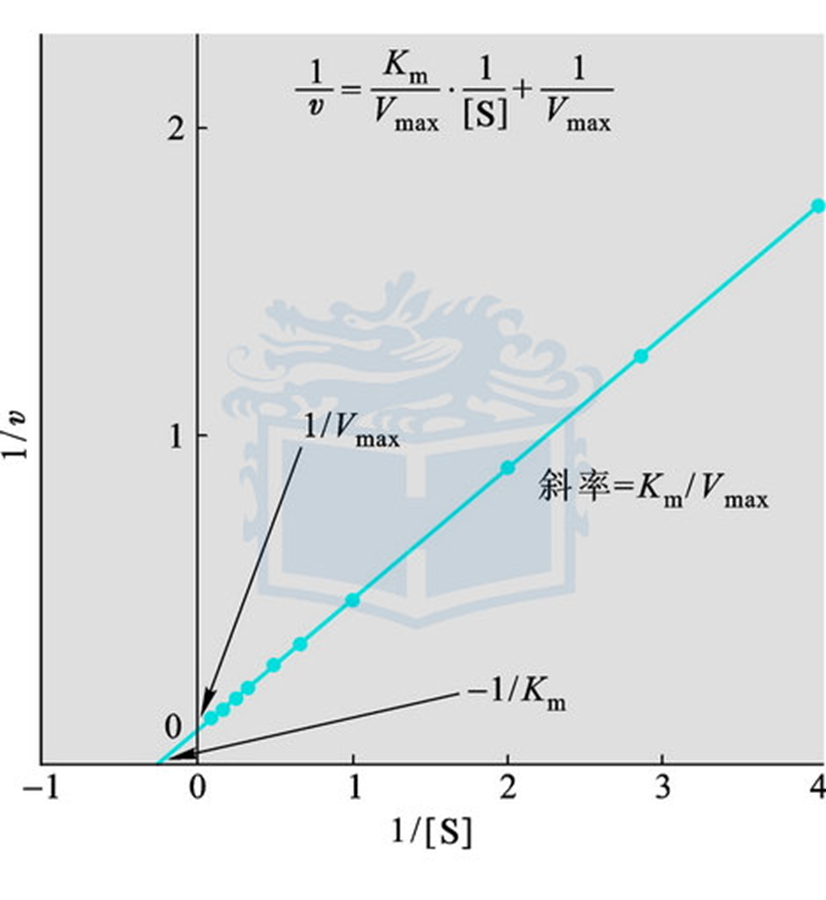
\includegraphics[width=0.7\linewidth]{Pics/双倒数法作图}
	\caption{双倒数法作图}
	\label{fig:双倒数法作图}
\end{figure}

其中:

\begin{itemize}
	\item 纵截距:$\dfrac{1}{V_{\text{max}}}$;
	\item 横截距:$-\dfrac{1}{K_{\text{m}}}$;
	\item 斜率:$\dfrac{K_{\text{m}}}{v_{\text{max}}}$。
\end{itemize}

缺陷:双倒数法作图会扩大误差。

\paragraph{Eadie-Hofstee作图}

\[v = -K_{\text{m}} \frac{v}{[\text{S}]} + v_{\text{max}}\]

以$\dfrac{v}{[\text{S}]}$为横轴、$v$为纵轴作图,其中:(\autoref{fig:eadie-hofstee})

\begin{figure}[htbp]
	\centering
	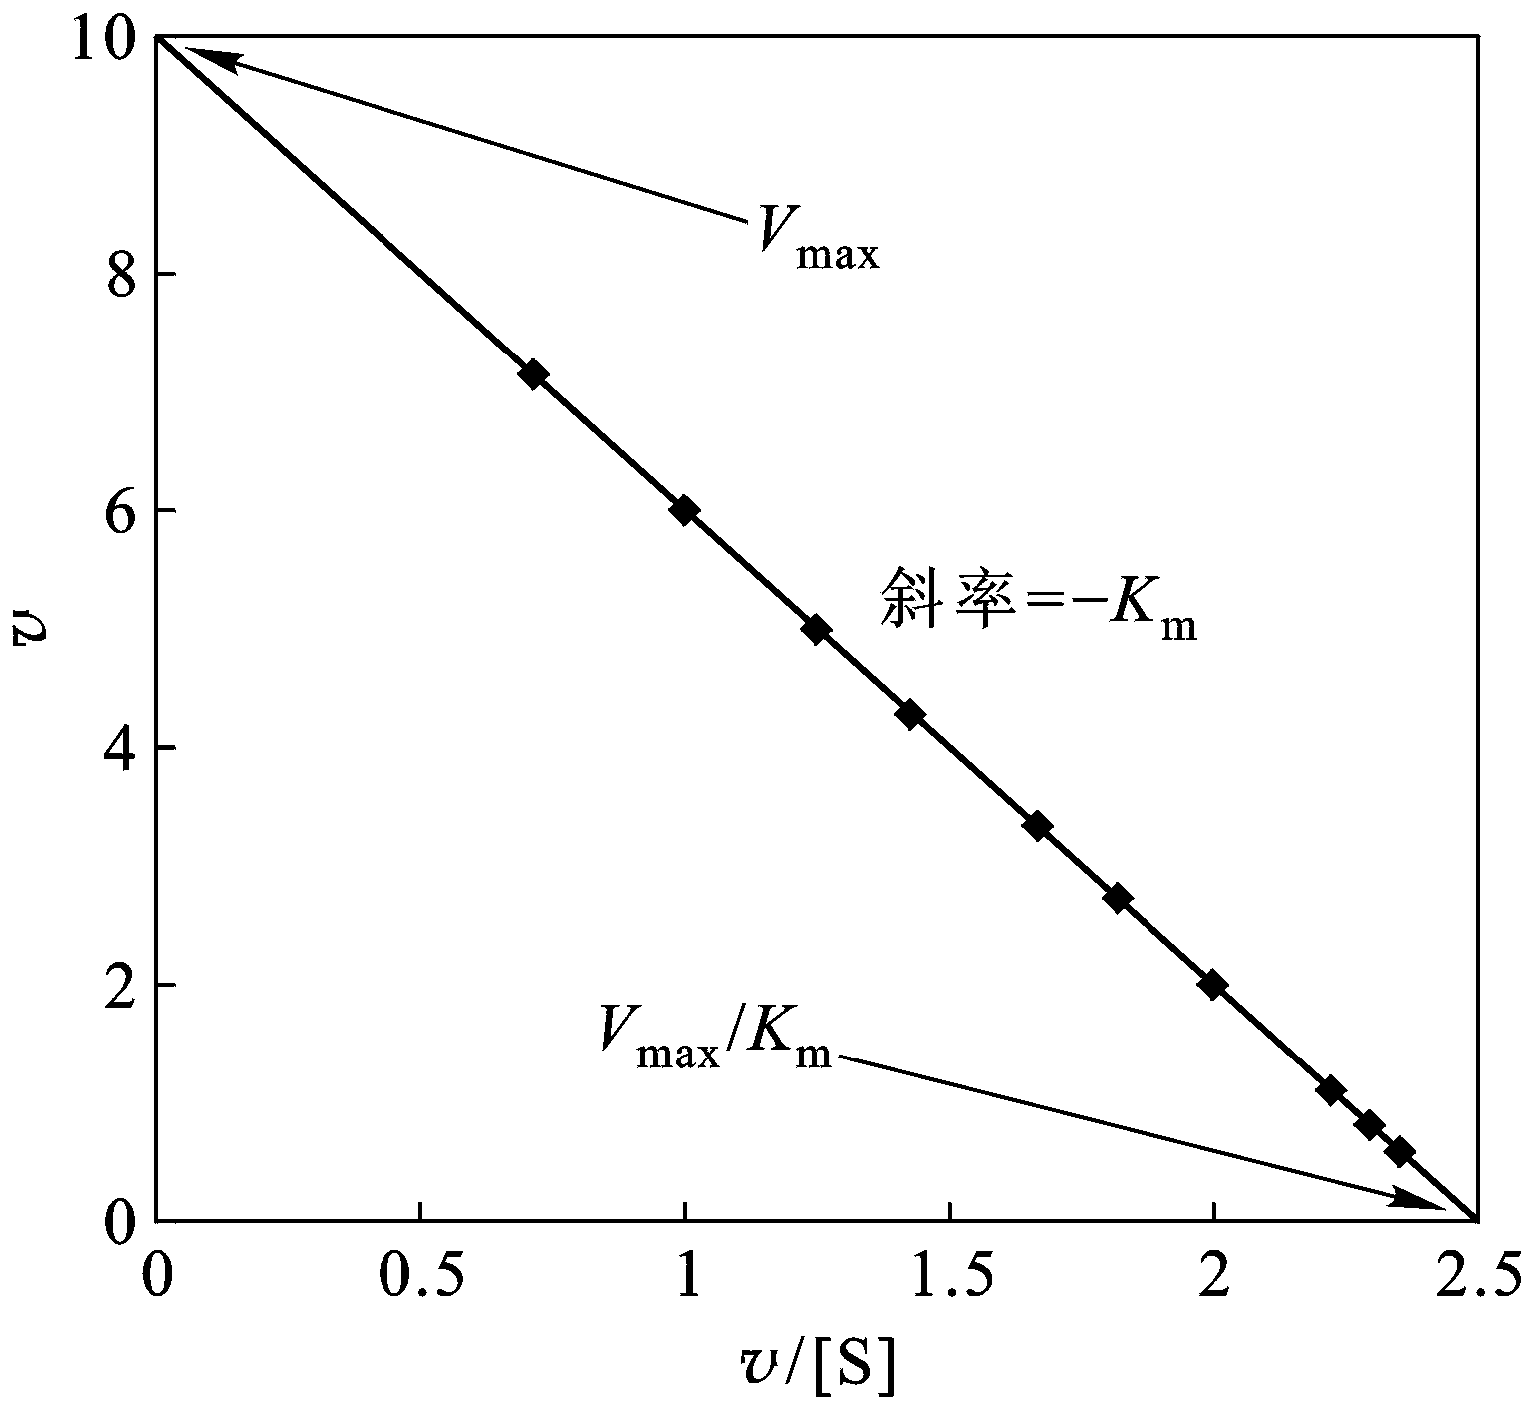
\includegraphics[width=0.5\linewidth]{Pics/Eadie-Hofstee作图}
	\caption{Eadie-Hofstee作图}
	\label{fig:eadie-hofstee}
\end{figure}

\begin{itemize}
	\item 纵截距:$v_{\text{max}}$;
	\item 横截距:$\dfrac{v_{\text{max}}}{K_{\text{m}}}$;
	\item 斜率:$-K_{\text{m}}$。
\end{itemize}

缺陷:同样会扩大误差,但没有双倒数法严重;$v$的误差会同时影响两个轴。

\paragraph{Hanes-Wolff作图}

\[\frac{[\text{S}]}{v} = \frac{1}{v_{\text{max}}} \cdot [\text{S}] + \frac{K_{\text{m}}}{v_{\text{max}}}\]

以$[\text{S}]$为横轴、$\dfrac{[\text{S}]}{v}$为纵轴作图,其中:(\autoref{fig:hanes-wolff})

\begin{figure}[htbp]
	\centering
	\includegraphics[width=0.5\linewidth]{"Pics/Hanes-Wolff 作图"}
	\caption{Hanes-Wolff作图}
	\label{fig:hanes-wolff}
\end{figure}

\begin{itemize}
	\item 纵截距:$\dfrac{K_{\text{m}}}{v_{\text{max}}}$;
	\item 横截距:$-K_{\text{m}}$;
	\item 斜率:$\dfrac{1}{v_{\text{max}}}$。
\end{itemize}

\paragraph{直接线性化作图}

\[v_{\text{max}} = \frac{v}{[\text{S}]} \cdot K_{\text{m}} + v\]

在直接线性化作图中,以$K_{\text{m}}$为横轴、$v_{\text{max}}$为纵轴,可以作出无数条直线。它们的交点坐标就是$(K_{\text{m}},V_{\text{max}})$。(\autoref{fig:直接线性化作图})

\begin{figure}[htbp]
	\centering
	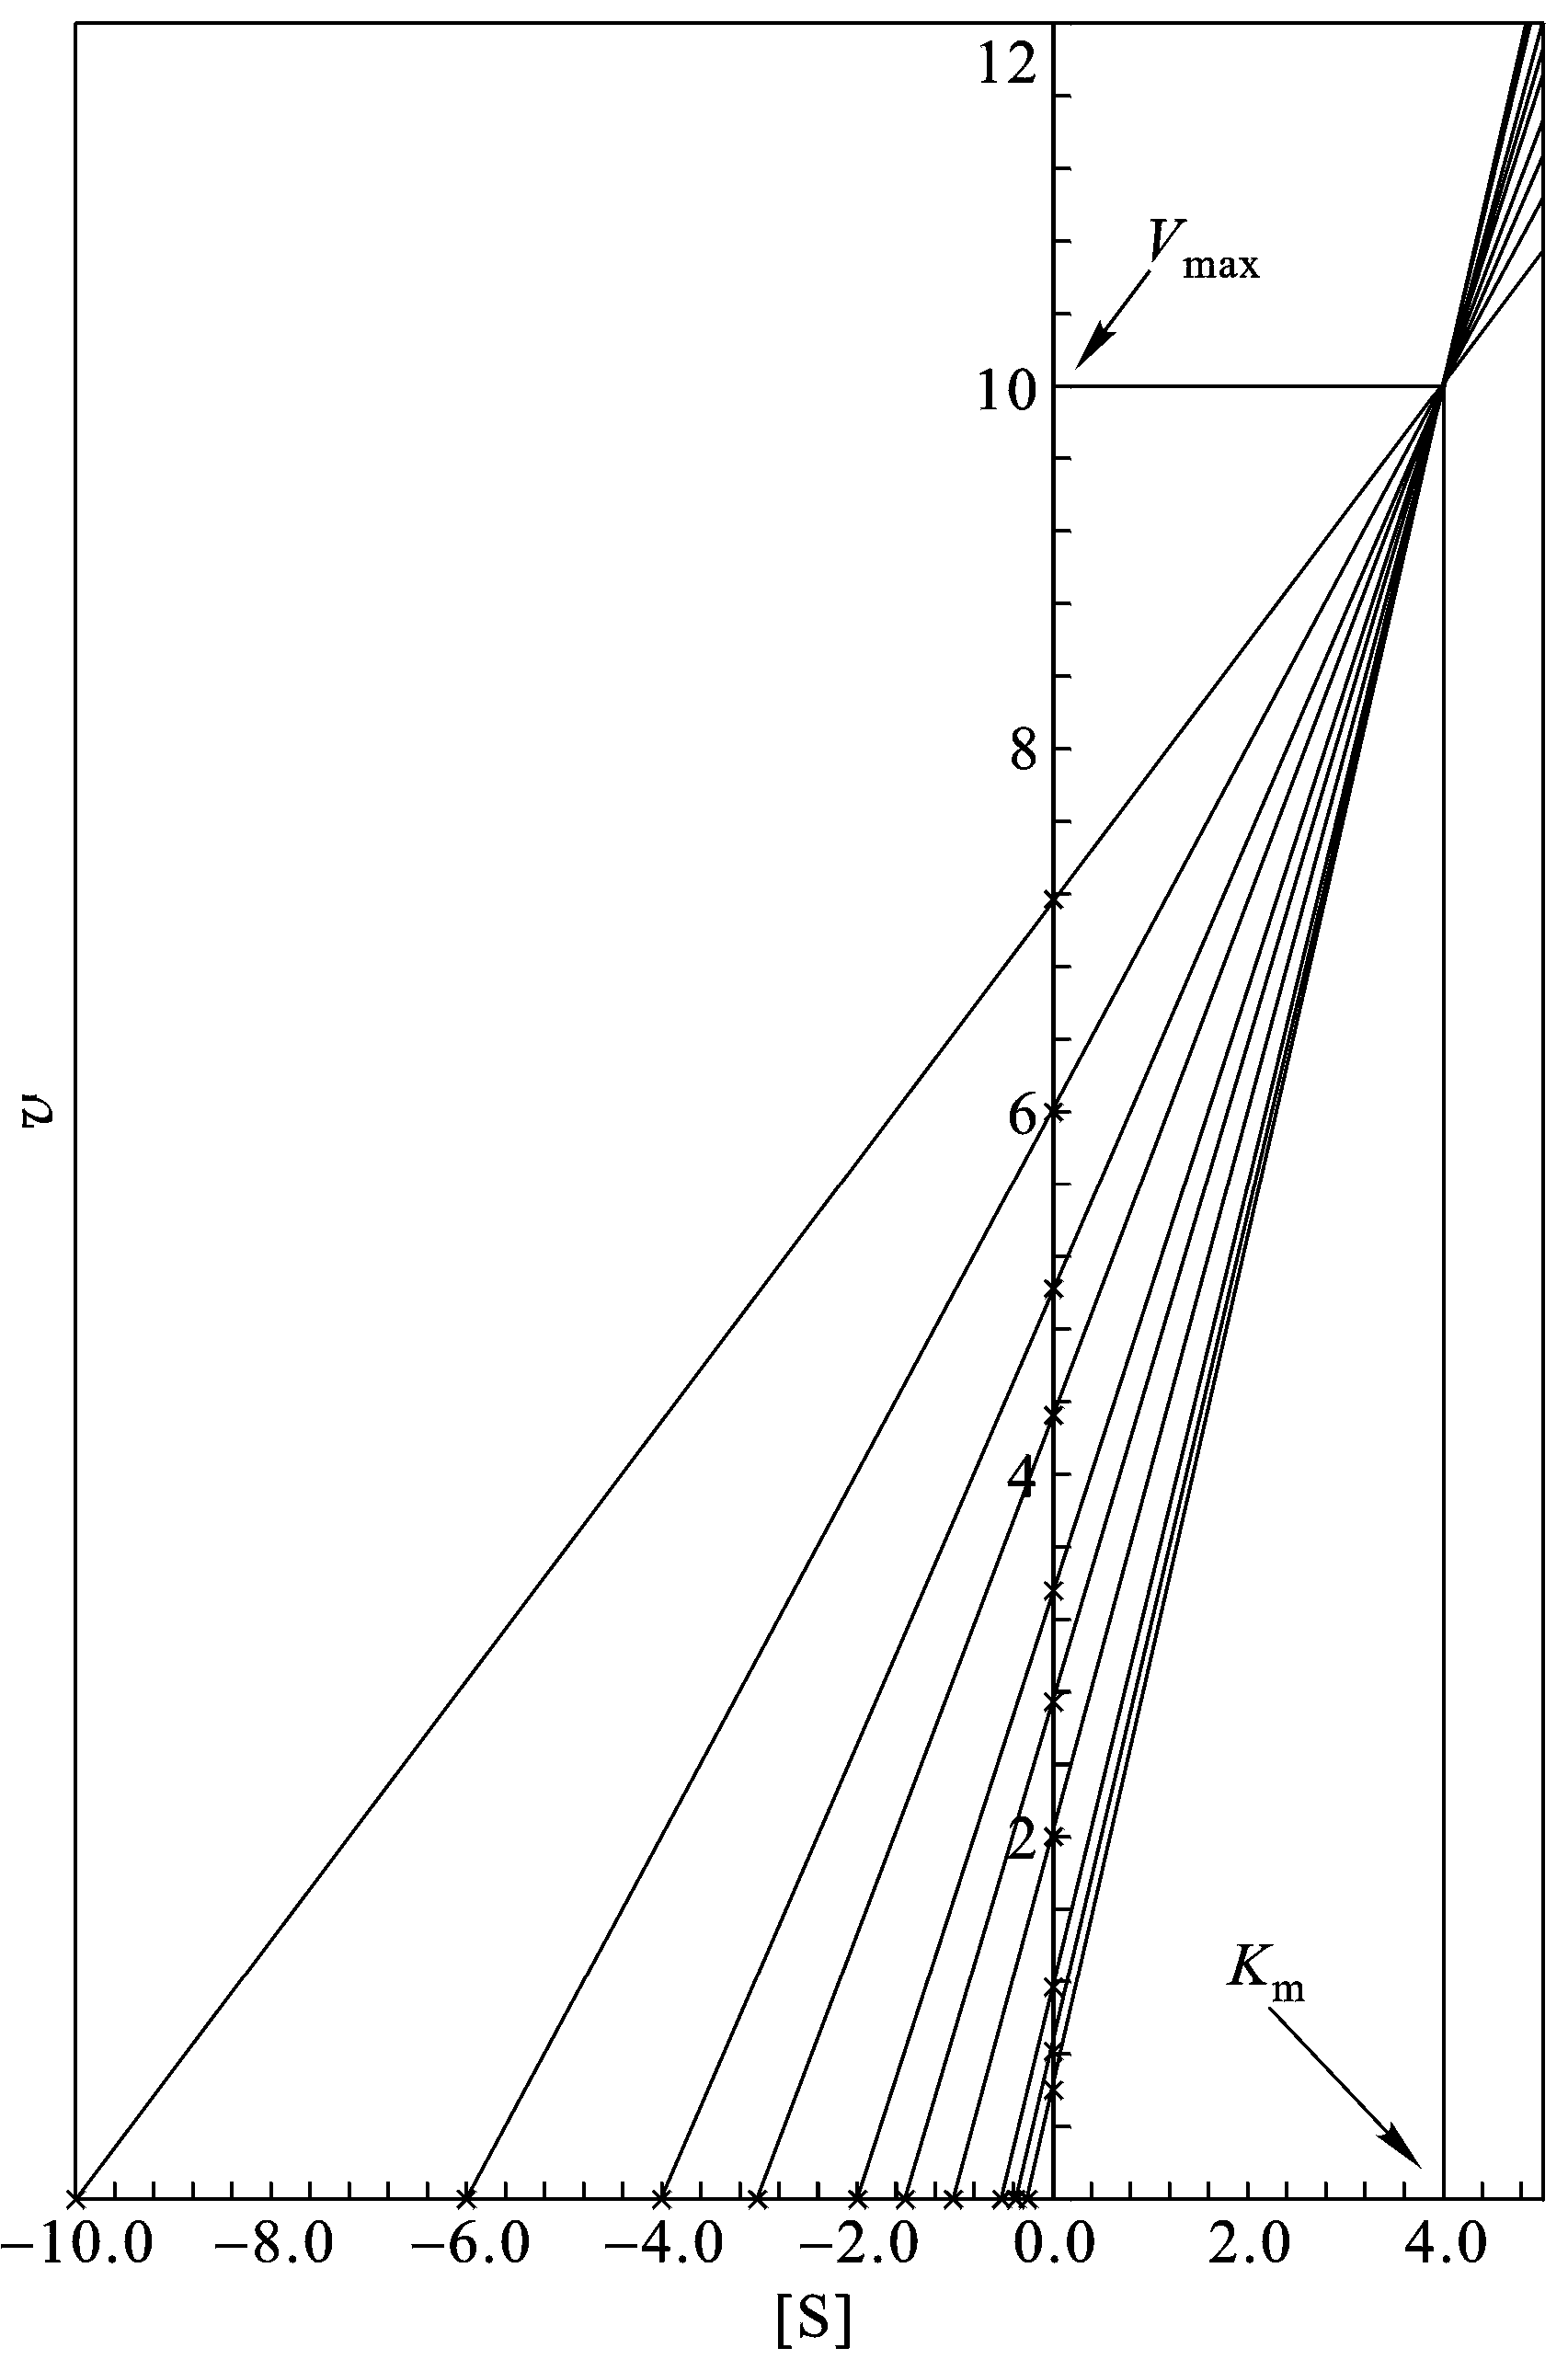
\includegraphics[width=0.5\linewidth]{直接线性化作图}
	\caption{直接线性化作图}
	\label{fig:直接线性化作图}
\end{figure}

\subsection{米氏酶抑制剂动力学}

酶的抑制剂分为可逆性抑制剂和不可逆性抑制剂两类(\autoref{fig:米氏酶抑制剂的分类})。不可逆抑制剂的作用有时间依赖性。

\begin{figure}[htbp]
	\centering
	\begin{forest}
		forest scheme
		[抑制剂
			[可逆性抑制剂
				[竞争性抑制剂]
				[非竞争性抑制剂]
				[反竞争性抑制剂]]
			[不可逆性抑制剂
				[基团特异性抑制剂]
				[底物类似物抑制剂]
				[过渡态类似物抑制剂]
				[自杀型抑制剂]]]
	\end{forest}
	\caption{米氏酶抑制剂的分类}
	\label{fig:米氏酶抑制剂的分类}
\end{figure}

\subsubsection{可逆性抑制剂}

在下面叙述中,定义:$\alpha=1+\dfrac{[\text{I}]}{K_{\text{I}}}$

三种可逆性抑制剂对酶的影响见\autoref{tab:三种可逆性抑制剂对酶的影响}。

\begin{table}[htbp]
	\centering
	\begin{tabularx}{\textwidth}{|c|C|C|C|}
		\hline
		\textbf{抑制剂类型} & \textbf{$K_{\text{m}}$} & \textbf{$V_{\text{max}}$} & \textbf{米氏方程} \\ \hline
		竞争性抑制剂 & 增加 & 不变 & $v = \frac{V_{\text{max}} [S]}{\alpha K_{\text{m}} + [S]}$ \\ \hline
		非竞争性抑制剂 & 不变 & 减少 & $v = \frac{V_{\text{max}} [S]}{(K_{\text{m}} + [S])\alpha}$ \\ \hline
		混合型抑制剂 & 增加 & 减少 & --- \\ \hline
		反竞争性抑制剂 & 减少 & 减少 & $v = \frac{V_{\text{max}} [S]}{K_{\text{m}} + [S]\alpha}$ \\ \hline
	\end{tabularx}
	\caption{三种可逆性抑制剂对酶的影响}
	\label{tab:三种可逆性抑制剂对酶的影响}
\end{table}

世上没有完全单纯的非竞争性抑制剂,而混合型抑制剂指的就是兼具非竞争性抑制剂和竞争性抑制剂特性的抑制剂。

\subsubsection{不可逆性抑制剂}

\subsection{别构酶的动力学}



\section[激素和信号转导]{激素及其受体介导的信号转导}

\subsection{激素的一般性质}

\subsubsection{激素的定义}

激素是一类非营养的、微量就能起作用的、在细胞之间传递信息的物质。它最显著的特征就是含量低。

分泌激素的细胞称内分泌细胞,受激素作用的细胞称靶细胞。根据作用的距离,把激素分为内分泌激素、神经内分泌激素、旁分泌激素、自分泌激素、内部分泌激素(\autoref{fig:hormone_types}、\autoref{tab:hormone_types})。

\begin{figure}[htbp]
	\centering
	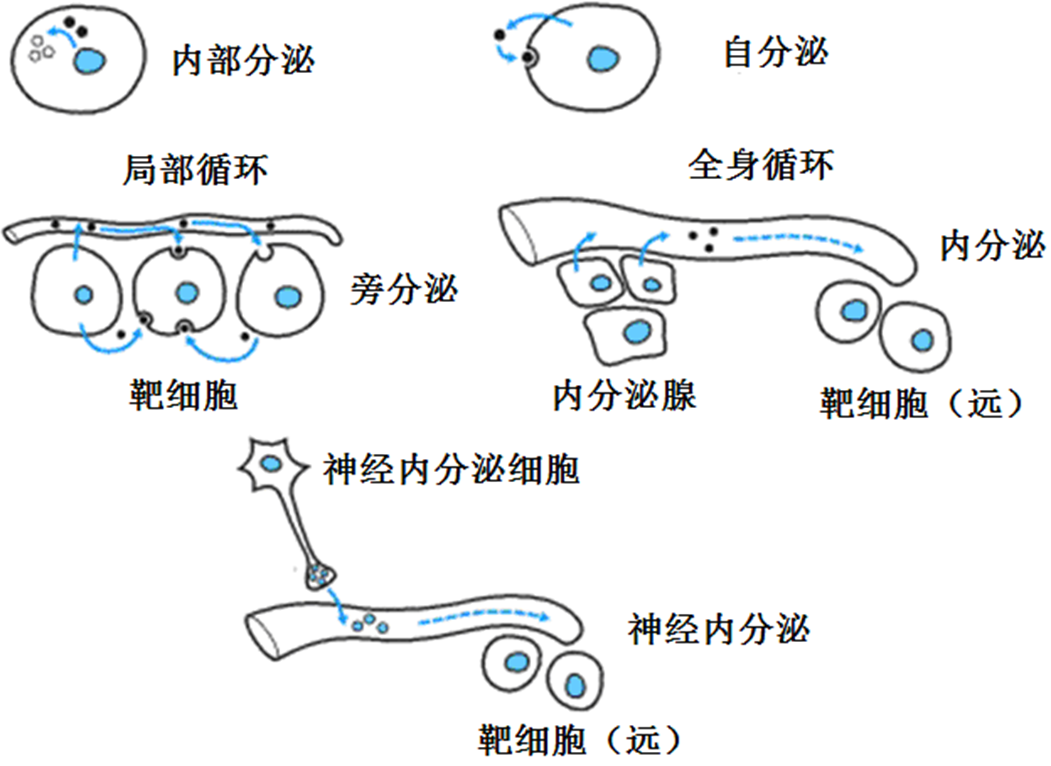
\includegraphics[width=0.7\linewidth]{Pics/激素作用类型}
	\caption{激素的5种分泌方式}
	\label{fig:hormone_types}
\end{figure}

\begin{table}[htbp]
	\centering
	\begin{tabularx}{\textwidth}{|c|X|X|}
		\hline
		\multicolumn{1}{|c|}{分泌方式} & \multicolumn{1}{c|}{作用对象} & \multicolumn{1}{c|}{举例} \\ \hline
		内分泌 & 较远的靶细胞 & 大多数激素 \\ \hline
		神经内分泌激素 & 同上,但是由特殊的神经内分泌细胞(同时也是神经细胞)分泌 & 哺乳动物下丘脑产生的激素 \\ \hline
		旁分泌激素 & 邻近的细胞 & 前列腺素、阿片肽、一些多肽生长因子 \\ \hline
		自分泌激素 & 原来分泌它的细胞 & 白介素-2、某些生长因子、某些原癌基因的产物 \\ \hline
		内部分泌激素 & 不分泌到胞外 & 胰岛素类生长因子结合蛋白3(IGFBP-3) \\ \hline
	\end{tabularx}
	\caption{激素的5种作用方式}
	\label{tab:hormone_types}
\end{table}

按照更广泛的激素的定义,生长因子、细胞因子和神经递质等细胞间信号分子也属于激素。

\subsubsection{激素的化学本质、分类}

按照来源和化学本质,把激素分为肽类或蛋白质激素、固醇类激素、氨基酸衍生物激素、脂肪酸衍生物激素。

\begin{itemize}
	\item 肽类或蛋白质激素种类最多,大小各异;
	\item 固醇类激素均衍生于胆固醇,包括维生素D、肾上腺皮质激素、性激素。所有固醇类激素都具有相同的环结构,但是空间取向不同,这就决定了激素作用的特异性;
	\item 氨基酸衍生物激素的前体是氨基酸,如Tyr、Trp;
		\begin{itemize}
			\item 衍生于Tyr的激素有:肾上腺素、去甲肾上腺素、甲状腺素;
			\item 衍生于Trp的激素有:5-羟色胺、褪黑素。
		\end{itemize}
	\item 脂肪酸衍生物激素衍生于脂肪酸,如花生四烯酸。这些激素包括:前列腺素、凝血恶烷、白三烯等。
\end{itemize}

按照溶解性质,激素可分为水溶性激素和脂溶性激素(\autoref{tab:hormone_differ})。

\begin{table}[h]
	\centering
	\begin{tabular}{|c|p{15em}|p{12em}|}
		\hline
		特征 & \multicolumn{1}{c|}{\makecell{脂溶性激素\\(如固醇类激素和甲状腺素)}} & \multicolumn{1}{c|}{\makecell{水溶性激素\\(如肽类激素和肾上腺素)}} \\ \hline
		合成后贮存 & 除了甲状激素以外很少见 & 是的 \\ \hline
		结合蛋白 & 总是 & 少见 \\ \hline
		半衰期 & 长(数小时或数天) & 短(几分钟) \\ \hline
		受体 & 细胞质或细胞核,极少数在细胞膜 & 总是在细胞膜 \\ \hline
		作用机制 & 直接 & 间接(通过第二信使) \\ \hline
	\end{tabular}
	\caption{脂溶性激素和水溶性激素的性质比较}
	\label{tab:hormone_differ}
\end{table}

\subsubsection{激素的生物合成}

\begin{enumerate}
	\item 肽类或蛋白质激素:绝大多数都是单一基因编码,少数是多个。

	前激素原$\xrightarrow{\text{内质网}}$激素原$\xrightarrow{\text{高尔基体}}$激素$\xrightarrow{\text{分泌小泡}}$出胞
	\item 固醇类激素合成主要发生在光面内质网,但少数反应在线粒体。
	\item 氨基酸衍生物是对氨基酸侧链修饰而成;
	\item 脂肪酸衍生物主要是花生四烯酸在特定酶催化下形成。
\end{enumerate}

\subsubsection{激素的定量}

放射免疫测定法(RIA)可以精确定量激素。

RIA的原理是同位素标记的激素(Ag*)和非同位素标记的激素(Ag)都能与特异性抗体结合,二者竞争结合位点。那么,一个只含有Ag*和Ab的体系,自然全都是Ag*-Ab复合物。当Ag加入,处于结合状态的Ag*和游离的Ag*比率$\displaystyle\frac{\text{Ag*-Ab}}{\text{Ag*}}$会下降。以$\displaystyle\frac{\text{Ag*-Ab}}{\text{Ag*}}$为纵轴、$(\text{Ag*}+\text{Ag})$为横轴作标准曲线。未知量的激素在同一体系中反应,可根据标准曲线获得激素的含量。(\autoref{fig:ria})

\begin{figure}[h]
	\centering
	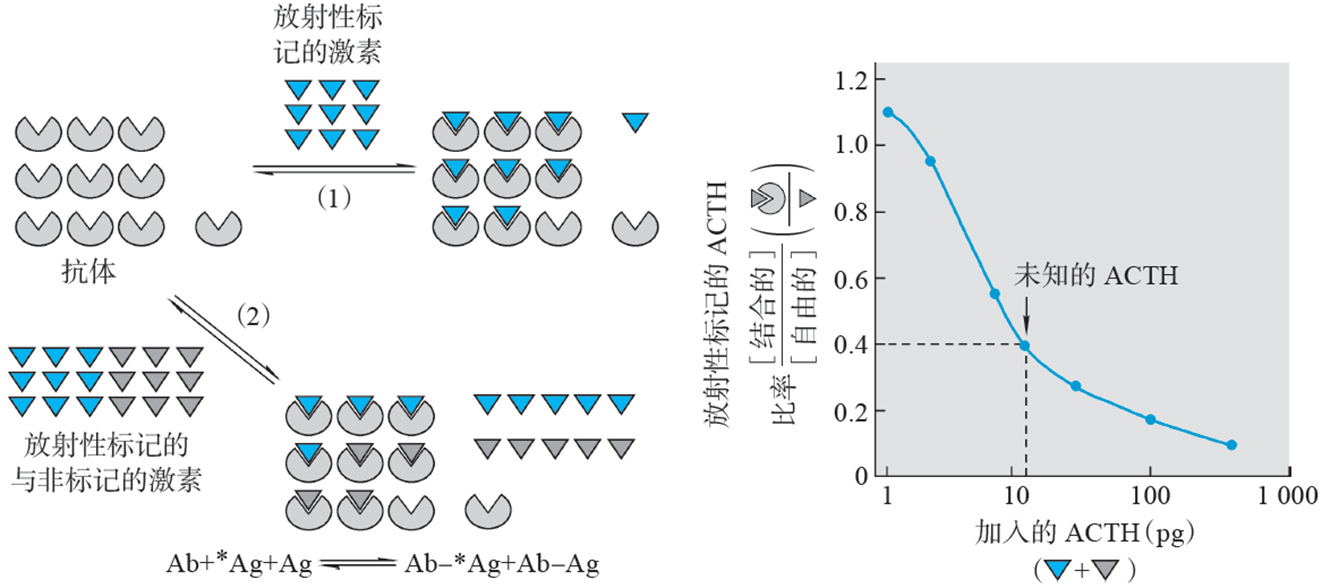
\includegraphics[width=\textwidth]{Pics/RIA}
	\caption{RIA的测定原理(以促肾上腺皮质激素ACTH为例)}
	\label{fig:ria}
\end{figure}

\subsection{激素作用的一般特征}

\subsubsection{特异性}

这是依赖于激素与特异性受体的结合实现的。


	\chapter{代谢生物化学}
		\section{生物能学}

\section{生物氧化}

\begin{table}[htbp]
	\centering
	\begin{tabularx}{\textwidth}{|c|c|C|}
		\hline
		抑制类型 & 抑制剂名称 & 作用位点或作用机制 \\ \hline
		\multirow{4}{*}{呼吸链抑制剂} & 鱼藤酮、安米妥、杀粉菌素 & 复合体 I \\ \cline{2-3} 
		& 萎锈灵 & 复合体 II \\ \cline{2-3} 
		& 抗霉素 A & 复合体 III \\ \cline{2-3} 
		& 氰化物、CO、H₂S、叠氮化物 & 复合体 IV \\ \hline
		\multirow{3}{*}{F₁F₀-ATP 合酶抑制剂} & 金轮霉素 & 抑制 F₁ \\ \cline{2-3} 
		& 寡霉素、杀黑星菌素 & 抑制 F₀ \\ \cline{2-3} 
		& DCCD & 阻止质子通过 F₀ 通道 \\ \hline
		\multirow{3}{*}{解偶联剂} & DNP、FCCP & 脂溶性质子载体 \\ \cline{2-3} 
		& 缬氨霉素 & 钾离子载体,破坏电势能 \\ \cline{2-3} 
		& 生热素 & 质子通道 \\ \hline
		ATP/ADP 交换体抑制剂 & 苍术苷、米酵菌酸 & 抑制线粒体基质内的 ATP 与细胞质内的 ADP 之间交换 \\ \hline
	\end{tabularx}
	\caption{生物氧化抑制剂}
	\label{tab:Biological_oxidation_inhibitor}
\end{table}
\section{糖酵解}

\subsection{糖酵解的全部反应}

糖酵解发生在细胞质基质,存在于所有细胞,包含十步反应。这十步反应分为两个阶段:(\autoref{fig:糖酵解纵览})
\begin{description}
	\item[引发阶段(投资阶段)] 一分子葡萄糖$\longrightarrow$2分子3-磷酸甘油醛,消耗2分子ATP。
	\item[产能阶段(获利阶段)] 2分子3-磷酸甘油醛$\longrightarrow$2分子丙酮酸,产生4分子ATP、2分子NADH。
\end{description}

\begin{figure}[htbp]
	\centering
	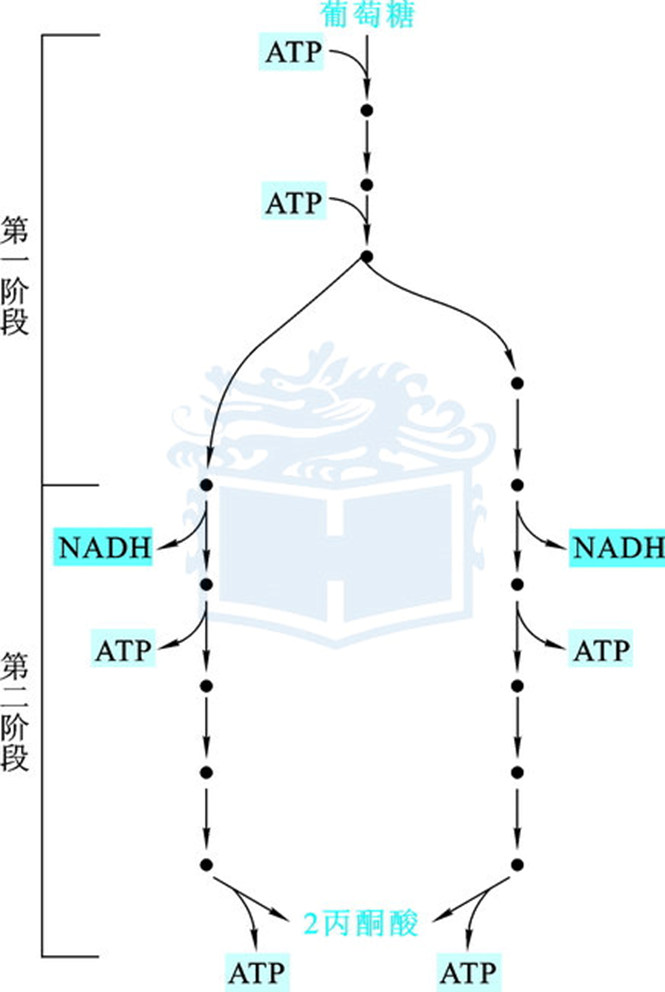
\includegraphics[width=0.4\linewidth]{Pics/糖酵解纵览}
	\caption{糖酵解纵览}
	\label{fig:糖酵解纵览}
\end{figure}

\begin{figure}[p]
	\centering
	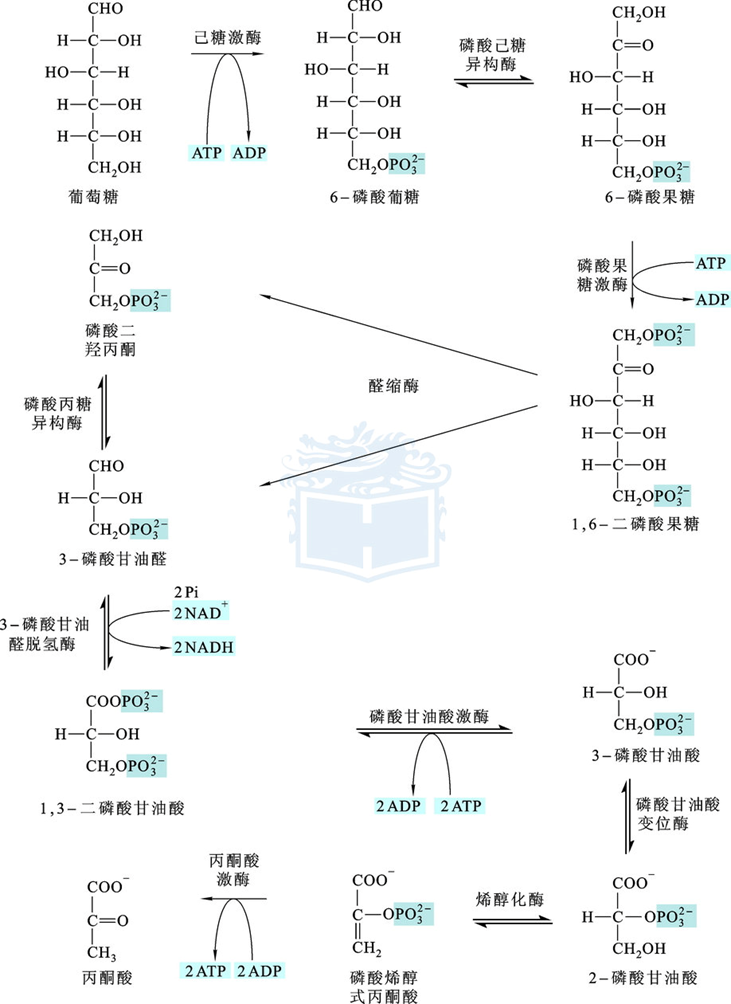
\includegraphics[width=\linewidth]{Pics/糖酵解的全部发硬}
	\caption{糖酵解的全部反应}
	\label{fig:all_reaction_glycolysis}
\end{figure}

下面分步介绍每步反应:

\subsubsection{葡萄糖的磷酸化}

\begin{center}
	葡萄糖+ATP$\xrightarrow[\text{己糖激酶或葡糖激酶}]{\ce{Mg^{2+}}}$6-磷酸葡糖+ADP
\end{center}

不可逆反应,由己糖激酶或葡糖激酶催化。己糖激酶利用诱导契合机制,避免ATP在活性中心的水解。

反应还需要\ce{Mg^{2+}},有时\ce{Mn^{2+}}可替代。细胞内所有涉及NTP或dNTP的反应都需要\ce{Mg^{2+}}。因为这些反应都依赖于一个亲核基团对磷酸基团P原子的亲核进攻。\ce{Mg^{2+}}和酶自带的碱性氨基酸残基可屏蔽解离状态的O原子所带的负电荷。如己糖激酶用K屏蔽$\gamma$-磷酸、用R屏蔽$\alpha$-磷酸的负电荷。

2-脱氧葡糖也可参与反应,生成2-脱氧-6-磷酸葡糖,是下一步异构反应的抑制剂。

葡萄糖磷酸化的意义:
\begin{itemize}
	\item 降低胞内葡萄糖浓度,有利于葡萄糖通过GLUT入胞;
	\item 提高葡萄糖的极性,避免葡萄糖离开细胞;
	\item 提高葡萄糖能量状态,使其不稳定。
\end{itemize}

己糖激酶和葡糖激酶的区别:(\autoref{tab:己糖激酶和葡糖激酶的区别})

\begin{table}[htbp]
	\centering
	\begin{tabularx}{\textwidth}{|c|C|C|}
		\hline
		特性 & 己糖激酶 & 葡糖激酶 \\ \hline
		存在 & 几乎所有的细胞 & 肝细胞、胰脏的$\upbeta$细胞 \\ \hline
		底物特异性 & 多数己糖 & 葡萄糖和 2-脱氧葡糖 \\ \hline
		对葡萄糖的$K_{m}$ & 低 & 高 \\ \hline
		$V_{max}$ & 低 & 高 \\ \hline
		产物反馈抑制 & G-6-P反馈抑制 & 不受G-6-P反馈抑制 \\ \hline
		基因表达 & 组成酶 & 诱导酶 \\ \hline
	\end{tabularx}
	\caption{己糖激酶和葡糖激酶的区别}
	\label{tab:己糖激酶和葡糖激酶的区别}
\end{table}

\begin{itemize}
	\item 己糖激酶是组成酶,与葡萄糖亲和力较高,能保证葡萄糖持续进入细胞;
	\item 葡糖激酶是诱导酶,与葡萄糖亲和力较低,血糖较高时才被诱导表达。
\end{itemize}

\subsubsection{6-磷酸葡糖的异构}

\begin{center}
	\ce{\text{6-磷酸葡糖} <=>[Mg^{2+}][\text{磷酸己糖异构酶}] \text{6-磷酸果糖}}
\end{center}

\subsection{NADH和丙酮酸的命运}

\subsubsection{有氧条件}

\paragraph{NADH}

有氧状态下,NADH将会把电子转移给呼吸链,产生更多ATP。
\begin{itemize}
	\item 在原核细胞,NADH很容易就可以到达呼吸链,因为呼吸链在细胞膜上;
	\item 在真核细胞,NADH要通过线粒体内膜就要经过专门的穿梭系统。
\end{itemize}

线粒体内膜上有3-磷酸甘油穿梭系统和苹果酸-天冬氨酸穿梭系统。脑细胞主要是前者, 肝细胞主要是后者。

\begin{description}
	\item[3-磷酸甘油穿梭系统] 如\autoref{fig:3-磷酸甘油穿梭系统},这种穿梭方式相当于把2个高能电子给了FAD,原本能产生2.5个ATP,现在只能产生1.5个。
	
	\begin{figure}[htbp]
		\centering
		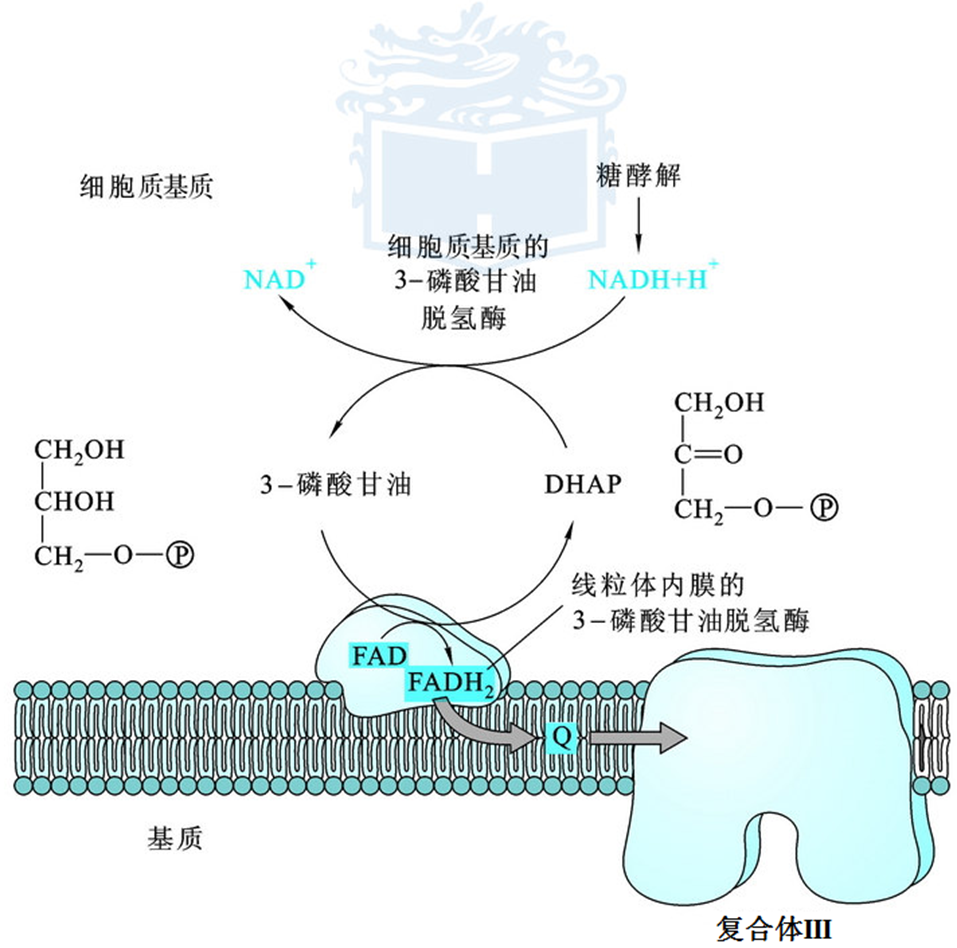
\includegraphics[width=0.7\linewidth]{Pics/3-磷酸甘油穿梭系统}
		\caption{3-磷酸甘油穿梭系统}
		\label{fig:3-磷酸甘油穿梭系统}
	\end{figure}
	
	\item[苹果酸-天冬氨酸穿梭系统] 如\autoref{fig:苹果酸-草酰乙酸穿梭系统},这一穿梭系统相当于用苹果酸把NADH的氢带进线粒体,最终可以无损耗地生成2.5个ATP。
	
	\begin{figure}[htbp]
		\centering
		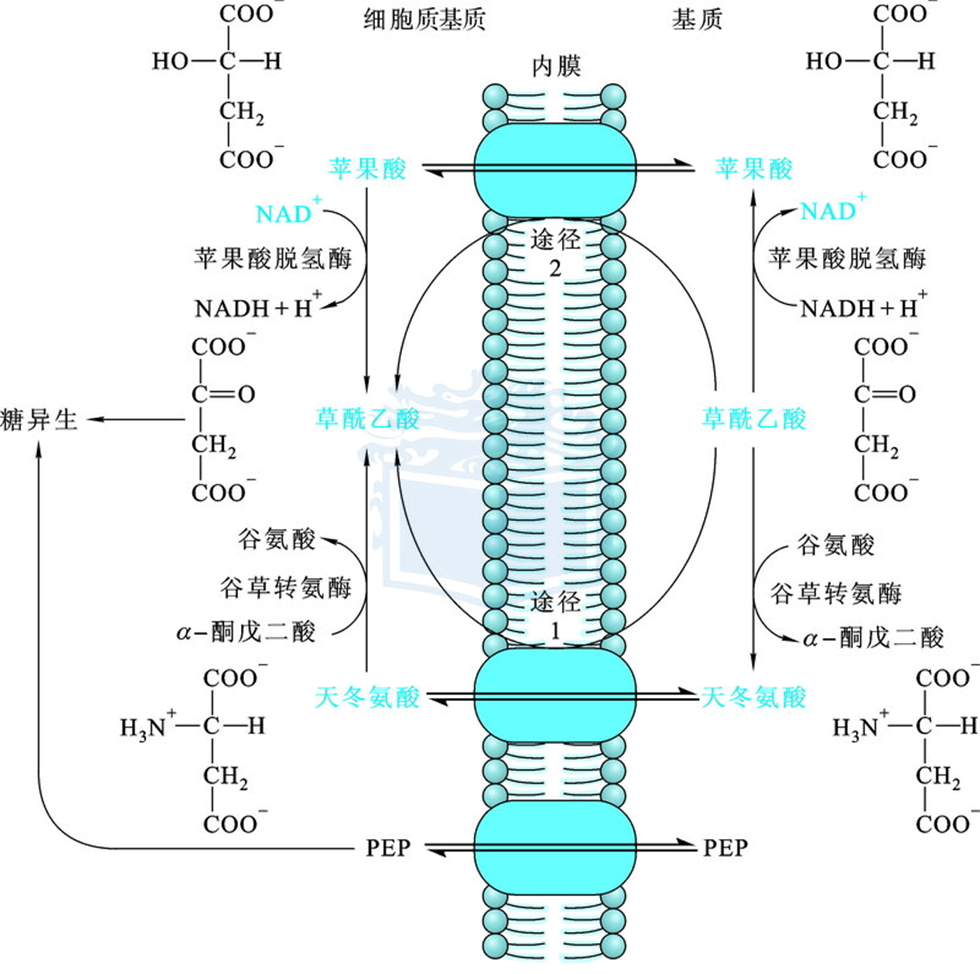
\includegraphics[width=0.9\linewidth]{Pics/苹果酸-草酰乙酸穿梭系统}
		\caption{苹果酸-草酰乙酸穿梭系统}
		\label{fig:苹果酸-草酰乙酸穿梭系统}
	\end{figure}
	
\end{description}

\paragraph{丙酮酸}

有氧条件下,丙酮酸将通过线粒体内膜上的丙酮酸转运蛋白,被线粒体基质内的丙酮酸脱氢酶系氧化成乙酰CoA。

\subparagraph{丙酮酸脱氢酶系的组成}

\begin{table}[htbp]
	\centering
	\begin{tabularx}{\textwidth}{|c|c|c|X|}
		\hline
		\textbf{酶} & \textbf{缩写} & \textbf{辅因子} & \multicolumn{1}{c|}{\textbf{催化反应}} \\ \hline
		丙酮酸脱氢酶 & E1 & TPP、Mg & 丙酮酸氧化脱羧 \\ \hline
		二氢硫辛酸转乙酰酶 & E2 & 硫辛酸、CoA & 氧化型硫辛酰胺的还原、羟乙基氧化为乙酰基、乙酰基的两次转移 \\ \hline
		二氢硫辛酸脱氢酶 & E3 & FAD、NAD$^{+}$ & 氧化型硫辛酰胺的再生 \\ \hline
	\end{tabularx}
	\caption{丙酮酸脱氢酶系的组成}
	\label{tab:丙酮酸脱氢酶系的组成}
\end{table}

丙酮酸脱氢酶系的反应如\autoref{fig:丙酮酸脱氢酶系}所示。

\begin{figure}[htbp]
	\centering
	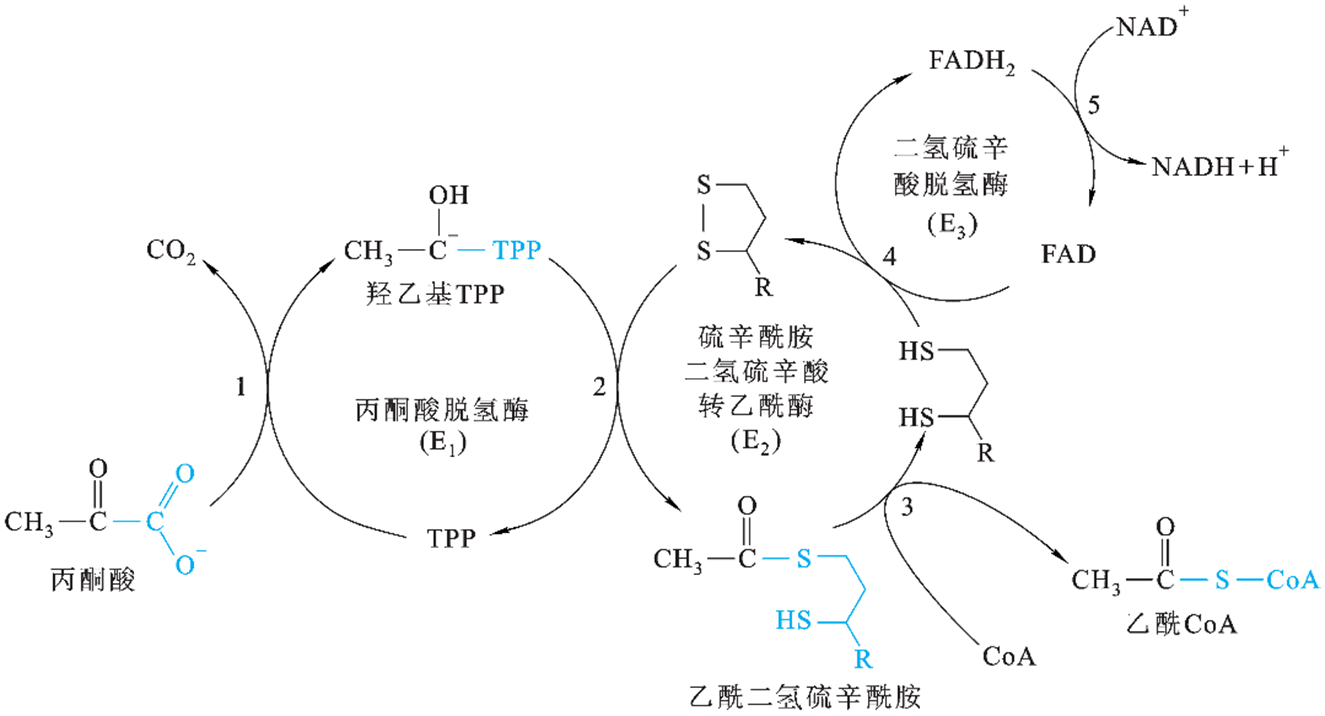
\includegraphics[width=\textwidth]{Pics/丙酮酸脱氢酶系}
	\caption{丙酮酸脱氢酶系}
	\label{fig:丙酮酸脱氢酶系}
\end{figure}

亚砷酸(砒霜的成分之一),能与还原型亚硫酰胺形成共价化合物(\autoref{fig:砒霜的毒性机理}),抑制整个丙酮酸脱氢酶系。它同样可抑制在三羧酸循环中的$\alpha$-酮戊二酸脱氢酶系中类似的反应。

\begin{figure}[htbp]
	\centering
	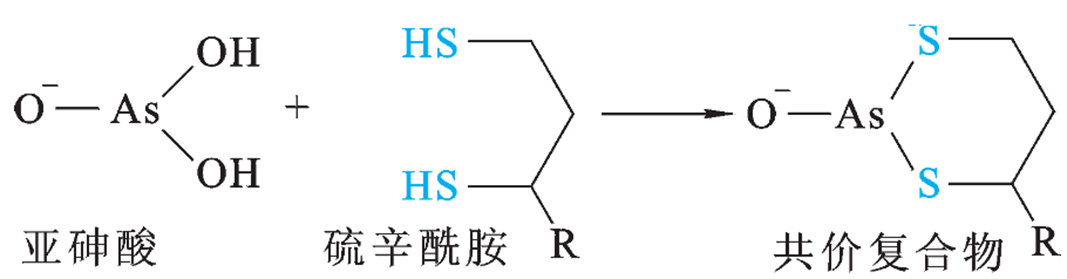
\includegraphics[width=0.5\linewidth]{Pics/砒霜有毒}
	\caption{砒霜的毒性机理}
	\label{fig:砒霜的毒性机理}
\end{figure}

\subsubsection{无氧条件}

无氧条件下,丙酮酸和NAD$^{+}$的命运是相互联系的。(\autoref{fig:丙酮酸的去路})不同生物使用的反应或许不同,但最终目的都是确保NADH变为NAD$^{+}$,即NAD$^{+}$再生。因为无氧条件下三羧酸循环不能进行。NADH不能消耗,最终将导致NAD$^{+}$耗尽,连糖酵解都无法进行。

\begin{figure}[htbp]
	\centering
	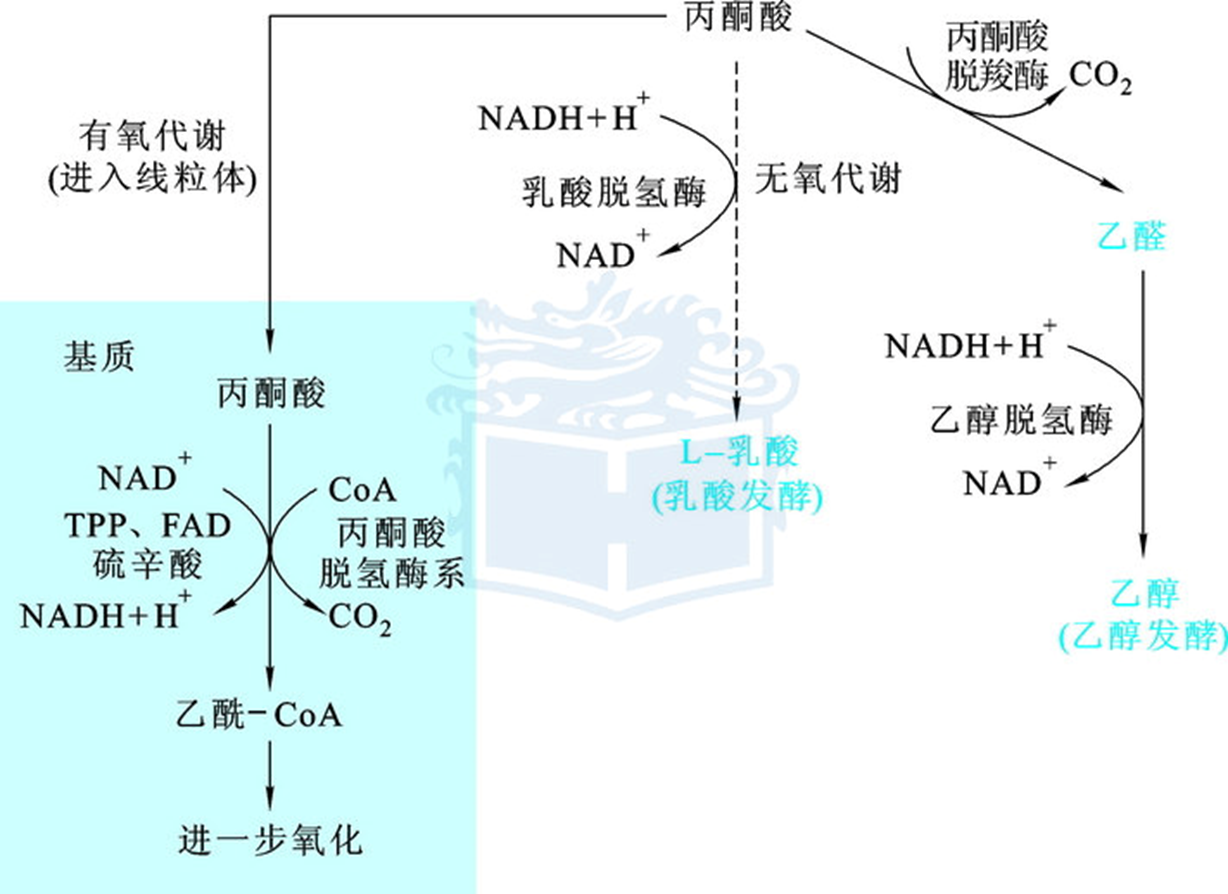
\includegraphics[width=0.7\linewidth]{Pics/丙酮酸的去路}
	\caption{丙酮酸的去路}
	\label{fig:丙酮酸的去路}
\end{figure}

\paragraph{乳酸发酵}

乳酸杆菌和其他一些微生物就是使用这条途径来完成NAD$^{+}$的再生。

高等动物的细胞在出现氧债的情况下,也会进行乳酸发酵,但是乳酸需要被运到肝细胞才能重新氧化成丙酮酸。哺乳动物红细胞无线粒体,故每时每刻都在进行乳酸发酵。

\paragraph{乙醇发酵}

许多微生物(如酿酒酵母)体内进行乙醇发酵。其中的丙酮酸脱羧酶依赖于TPP。

人体内虽然有乙醇脱氢酶,但是因为没有丙酮酸脱羧酶,故无法进行乙醇发酵。

\paragraph{其他形式的发酵}

有的微生物还可通过其他方式完成NAD$^{+}$的再生。无论是哪种形式的发酵,都是用NADH的电子去还原有机物罢了。

\begin{gs}[:不喝酒也醉酒的秘密]
	
	\hspace{2em}想象一下,吃碗面或薯片后竟然醉了!这不是玩笑,二战后,美国大兵查尔斯·斯瓦特就遇到了这种怪事。20年来,他没沾酒却总是醉醺醺的,肝脏也受尽折磨。直到1964年,他发现有个日本人和他同病相怜。25年后,医生终于诊断出他们得了“自动酿酒综合征”。原来,他们肠道里的酵母菌变异了,不断进行糖酵解和乙醇发酵。在医生建议下,斯瓦特服用了杀酵母的药物,直到1975年才恢复正常。
	
	\hspace{2em}医生诊断难,因为这种酵母菌本是肠道常客,谁会想到它能酿酒呢?至于变异原因,可能是广岛和长崎的核爆辐射导致的。
\end{gs}

\subsection{其他物质进入糖酵解}

\begin{figure}[htbp]
	\centering
	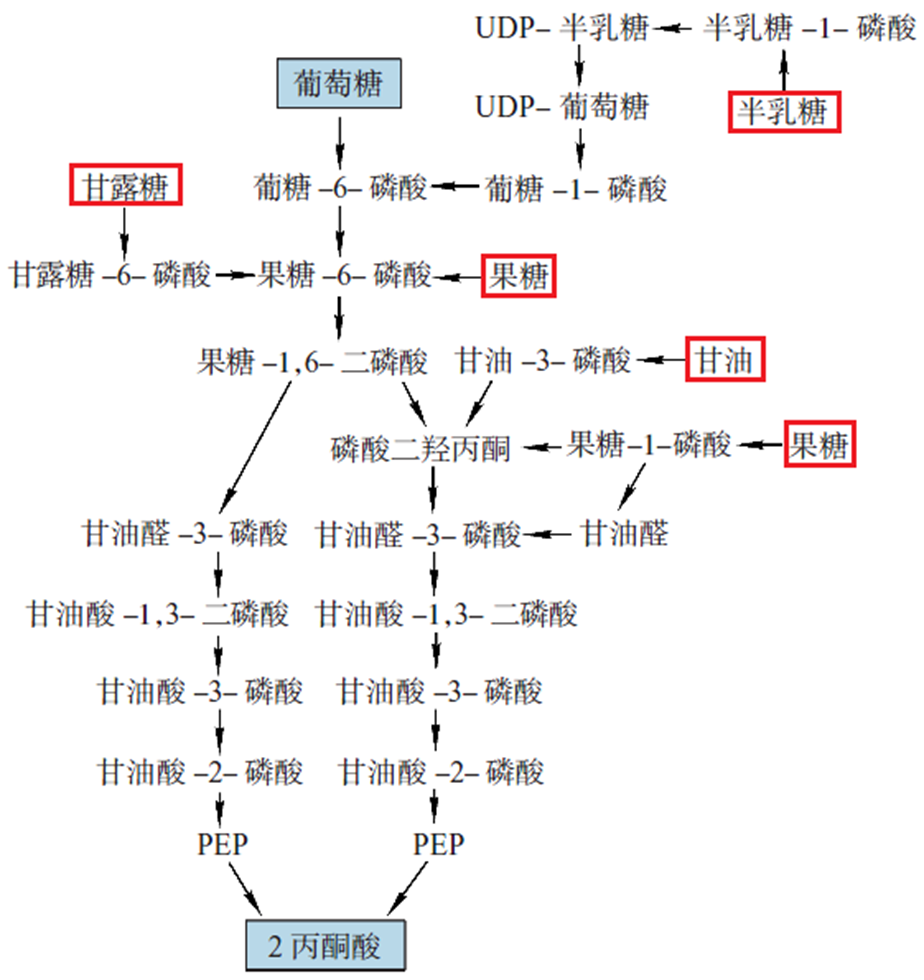
\includegraphics[width=0.8\linewidth]{Pics/其他物质进入糖酵解}
	\caption{其他物质进入糖酵解的途径}
	\label{fig:其他物质进入糖酵解的途径}
\end{figure}

\subsubsection{糖原}

糖原$\xrightarrow[\text{磷酸解}]{\text{糖原磷酸化酶a}}$1-磷酸葡萄糖$\xrightarrow{\text{磷酸葡糖变位酶}}$6-磷酸葡糖$\longrightarrow$糖酵解

\subsubsection{果糖}

果糖可通过两种方式进入糖酵解:
\begin{enumerate}
	\item (肌、肾)果糖$\xrightarrow{\text{己糖激酶}}$6-磷酸果糖$\longrightarrow$糖酵解
	\item (肝)果糖$\xrightarrow{\text{果糖激酶}}$1-磷酸果糖$\xrightarrow[\text{(醛缩酶B)}]{\text{1-磷酸果糖醛缩酶}}$磷酸二羟丙酮、D-甘油醛\\
	$\xrightarrow[\text{后者丙糖激酶}]{\text{前者TIM}}$3-磷酸甘油醛$\longrightarrow$糖酵解
\end{enumerate}

\subsubsection{甘露糖}

甘露糖$\xrightarrow{\text{己糖激酶}}$6-磷酸甘露糖$\xrightarrow{\text{磷酸甘露糖异构酶}}$6-磷酸果糖$\longrightarrow$糖酵解

\subsubsection{甘油}

甘油$\xrightarrow{\text{甘油激酶}}$3-磷酸甘油$\xrightarrow{\text{3-磷酸甘油脱氢酶}}$磷酸二羟丙酮$\xrightarrow{\text{磷酸丙糖异构酶}}$3-磷酸甘油醛$\longrightarrow$糖酵解

\subsubsection{半乳糖}

半乳糖进入糖酵解需要经过leloir途径(\autoref{fig:leloir})。

\begin{figure}[htbp]
	\centering
	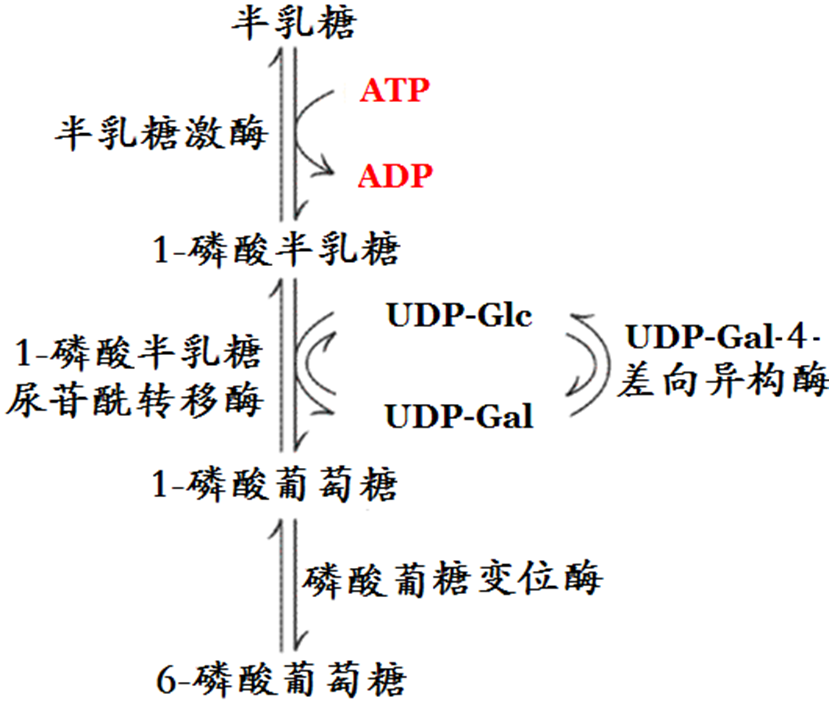
\includegraphics[width=0.4\linewidth]{Pics/Leloir途径}
	\caption{Leloir途径}
	\label{fig:leloir}
\end{figure}

\subsection{糖酵解的生理功能}

糖酵解较为普通的生理功能有:产ATP、为细胞内其他物质合成提供原料(\autoref{fig:糖酵解某些中间物的代谢流向})。下面介绍比较特别的功能。

\begin{figure}[htbp]
	\centering
	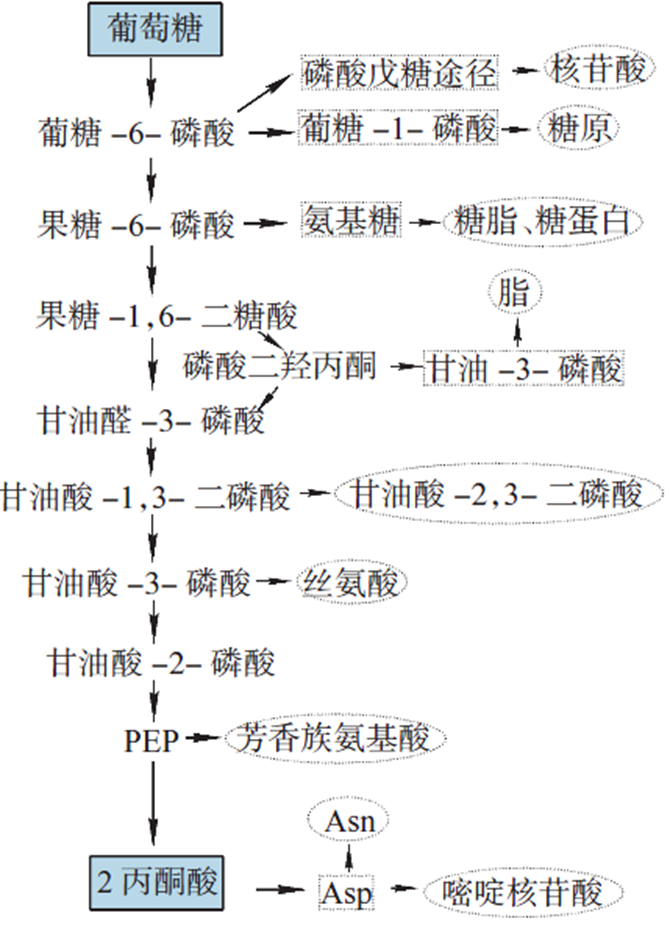
\includegraphics[width=0.4\linewidth]{Pics/糖酵解某些中间物的代谢流向}
	\caption{糖酵解某些中间物的代谢流向}
	\label{fig:糖酵解某些中间物的代谢流向}
\end{figure}

\subsubsection{癌细胞与糖酵解}

癌细胞生长速度很快,对能量需求高,常处于因血流不足而处在缺氧状态。受缺氧诱导,转录因子HIF-1$\upalpha$被激活,与DNA上缺氧应答元件结合,最后诱导参与糖酵解的酶和GLUT1、GLUT2的表达。

HIF-1$\upalpha$被激活的原理是:
\begin{itemize}
	\item 有氧条件下,该蛋白的一个Pro发生羟基化修饰,羟基的氧来源于氧气。这个羟基化使其容易被泛素化降解。
	\item 缺氧条件下,HIF-1$\upalpha$就可以稳定存在,作为转录因子诱导基因表达。
\end{itemize}

HIF-1$\upalpha$还可诱导血管内皮生长因子(VEGF)表达,促进新血管生长,为癌细胞供氧。

\subsubsection{糖酵解中一些酶的兼职功能}

\paragraph{磷酸己糖异构酶}

\begin{itemize}
	\item 兼职神经白介素;
	\item 作为自分泌运动因子。
\end{itemize}

\paragraph{3-磷酸甘油醛脱氢酶}

在细胞核中兼职尿嘧啶-DNA糖苷酶,参与DNA的碱基切除修复。

\paragraph{烯醇化酶}

\begin{itemize}
	\item 在细菌体内作为RNA降解体的一部分;
	\item 在真核生物体内,参与线粒体tRNA的运输;
	\item 在某些哺乳动物体内,作为细胞表面的受体结合纤维蛋白溶酶原和胞外基质,促进正常的细胞迁移;
	\item 病原体的烯醇化酶也有结合纤维蛋白溶酶原的活性,利用纤溶酶途径促进宿主组织的水解,有利于入侵;
\end{itemize}

\paragraph{醛缩酶}

\begin{itemize}
	\item 作为胞内葡萄糖水平高低的感应器,帮助细胞实时探测葡萄糖水平。
	\item 通过改变AMP激活的蛋白激酶(AMPK)的活性对细胞内葡萄糖水平的变化及时作出反应:促进多种蛋白质(如regulator、V型ATP酶、轴蛋白和肝激酶B1(LKB1)等)聚合在一起,最终激活依赖溶酶体的AMPK途径,进而激活AMPK。AMPK可催化胞内多种限速酶的磷酸化修饰,导致多条合成代谢途径的关闭。
\end{itemize}

\subsection{糖酵解的调节}


	\chapter{分子生物学}
		
分子生物学的核心是中心法则(\autoref{fig:genetic_central_dogma})。除此之外,朊病毒通过催化其他正常蛋白质发生构象变化来实现“复制”,和传统意义的复制不太一样。

对于分子生物学的知识,原核生物重点记忆,真核生物关注和原核生物的不同点,古菌了解即可。

\begin{figure}[htbp]
	\centering
	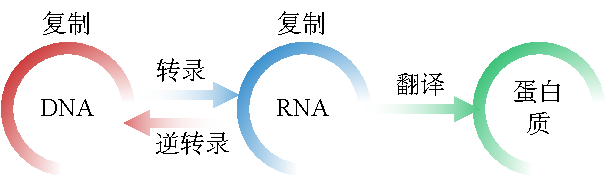
\includegraphics{中心法则.pdf}
	\caption{中心法则}
	\label{fig:genetic_central_dogma}
\end{figure}


\section{DNA复制}

\subsection{DNA复制的一般特征}

DNA复制的一般特征包括:

\begin{description}
	\item[需要模板、dNTPs、\ce{Mg^{2+}}] 其中\ce{Mg^{2+}}的作用是屏蔽磷酸基团的负电荷。有时少量的dUTP会掺入DNA。
	\item[模板DNA需要解链] 暴露出在双螺旋内部的碱基。
	\item[半保留复制] Meselson和Stahl的实验证明了这一点,注意使用的是\ce{CsCl}平衡密度梯度离心。(\autoref{fig:Meselson和Stahl的证明DNA半保留复制的实验流程})
	\item[通常需引物] 由DNA聚合酶的所致。引物多为RNA,少数为蛋白质,PCR的引物为DNA。一种噬菌体的DNA复制不需要引物。
	\item[复制方向永远是5$\prime$$\longrightarrow$3$\prime$] 可以向复制体系中加入ddNTP来验证。若为5$\prime$$\longrightarrow$3$\prime$,则会掺入ddNTP,进而导致末端终止;若为3$\prime$$\longrightarrow$5$\prime$,则ddNTP根本没机会掺入,复制不终止。(\autoref{fig:证明DNA复制方向的实验})
	\item[起点固定] DNA复制的起点即复制起始区。详后。
	\item[多双向,少单向] 从复制子开始向两侧复制,是为双向复制。
	\item[半不连续性] 因dNTP只能5$\prime$$\longrightarrow$3$\prime$加入(\autoref{fig:证明DNA复制方向的实验}),故有前导链、后随链之分。后随链产生冈崎片段。
	\item[高度忠实性] 在进行DNA复制时,细胞内依赖一系列校对与纠错机制来保证DNA复制具有远高于其他核酸合成反应的忠实性。
	\item[高度进行性] 进行性指DNA聚合酶从与模板结合到解离这段时间内,催化DNA分子延长的核苷酸数。参与DNA复制的,一定是细胞内进行性高的DNA聚合酶。
\end{description}

\begin{figure}[htbp]
	\centering
	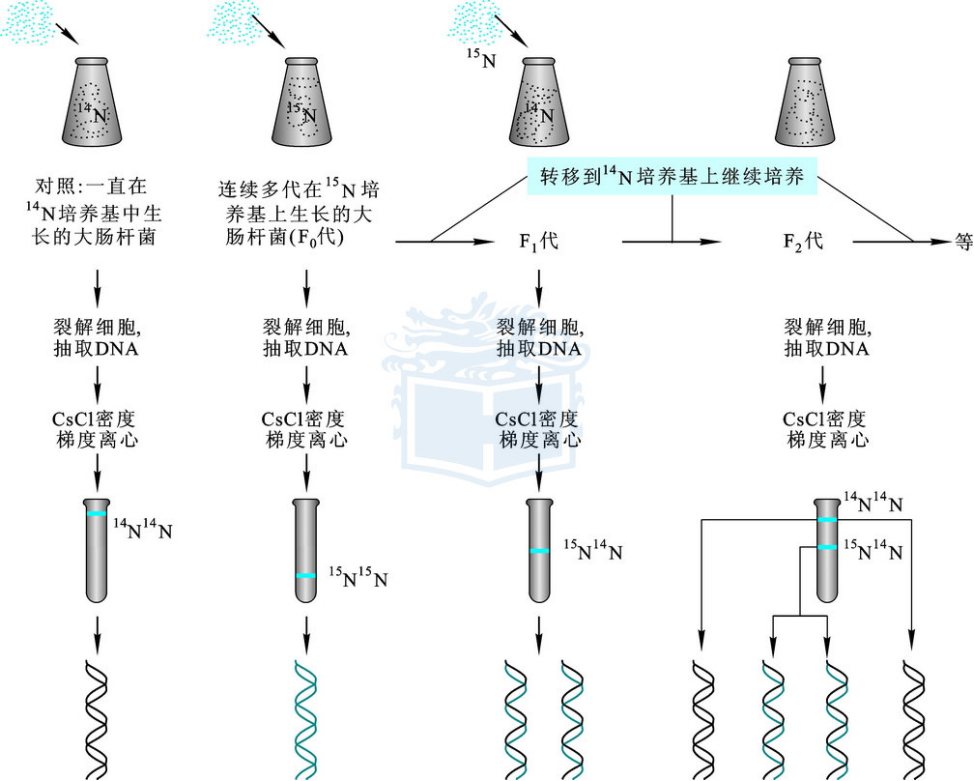
\includegraphics[width=\linewidth]{证明DNA半保留复制的实验.png}
	\caption{Meselson和Stahl的证明DNA半保留复制的实验流程}
	\label{fig:Meselson和Stahl的证明DNA半保留复制的实验流程}
\end{figure}

\begin{figure}[htbp]
	\centering
	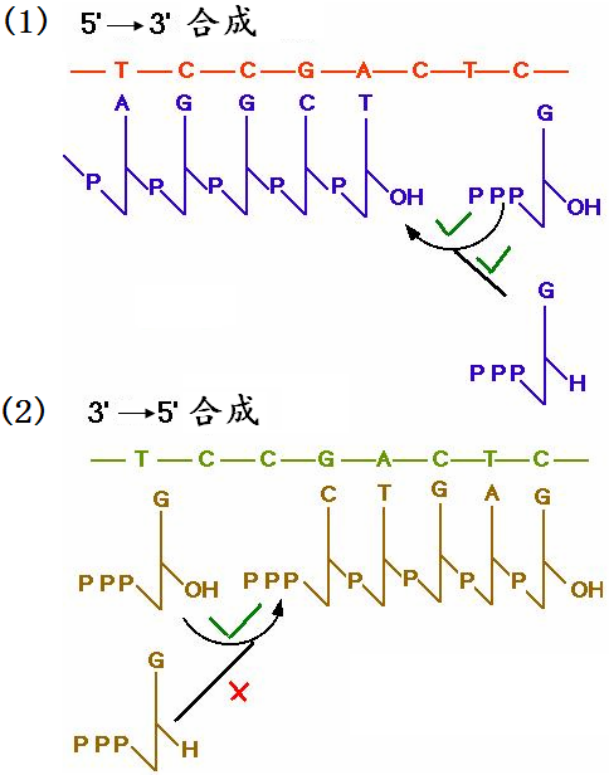
\includegraphics[width=0.4\linewidth]{证明DNA复制方向的实验.png}
	\caption{证明DNA复制方向的实验}
	\label{fig:证明DNA复制方向的实验}
\end{figure}

\subsubsection{不需要引物的生物}

DNA复制需要引物的生物学意义是,利于形成稳定的双螺旋结构,保证后续复制的忠实性。而这种在深海火山口附近细菌内的噬菌体,希望引入更多的突变,以求获得有利于生存的性状。

这种噬菌体编码的DNA聚合酶同时具有引发酶、DNA聚合酶、RNA聚合酶的特性。

\subsubsection{复制起始区和复制子}

复制起始区是作为DNA复制起点的一段碱基序列,具有如下特点:
\begin{description}
	\item[多个短的重复序列]
	\item[被复制起始区结合蛋白识别] 如DnaA(细菌)、Orc1-Orc6(真核)、Orc1/Cdc6(古菌)。
	\item[富含AT碱基对] AT碱基对之间只有2条氢键,比GC(3条)少,有利于解链。
\end{description}

细菌的DNA复制起始区只有一个,而真核生物和部分古菌有多个。

每个复制起始区构成一个复制子。DNA复制时,解链形成复制叉。(\autoref{fig:复制叉})

\begin{figure}[htbp]
	\centering
	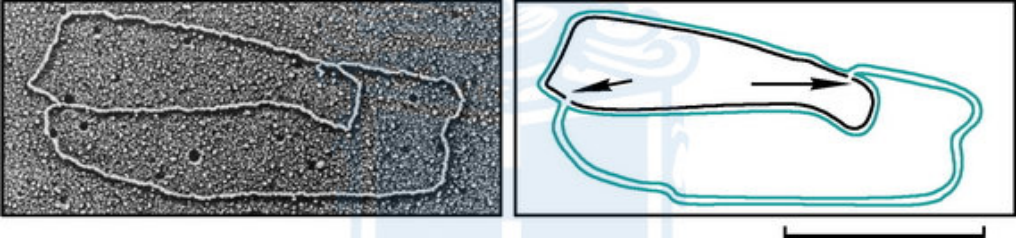
\includegraphics[width=0.7\linewidth]{复制叉.png}
	\caption{复制叉}
	\label{fig:复制叉}
\end{figure}

\subsection{参与DNA复制的主要酶和其他蛋白质}

DNA复制主要涉及DNA聚合酶、DNA解链酶、单链DNA结合蛋白、DNA引发酶、DNA拓扑异构酶、DNA连接酶、端粒酶等。

\subsubsection{DNA聚合酶}

DNA聚合酶是依赖于DNA的DNA聚合酶。反应把dNTP转变成dNMP和PPi,相当于消耗了两个ATP。

DNA聚合酶的共性:

\begin{itemize}
	\item 不能催化DNA的从头合成,故DNA复制需要引物;
	\item 只能催化DNA从5$\prime$$\longrightarrow$3$\prime$合成;
	\item 类似于右手的构象:手指、手掌、拇指三个结构域;
	\item 都需要2个\ce{Mg^2+},一个随\ce{dNTP}进入活性中心、另一个本来就在那里。它们与活性中心的3个Asp残基结合。所有物种中,这3个Asp残基都是高度保守的。
\end{itemize}

\paragraph{细菌的DNA聚合酶}

大肠杆菌中发现了五种DNA聚合酶,用罗马数字表示为DNA聚合酶I、II、III、IV、V。

\begin{table}[htbp]
	\centering
	\begin{tabularx}{\textwidth}{|c|c|C|C|}
		\hline
		性质 & DNA聚合酶I & DNA聚合酶II & DNA聚合酶III \\
		\hline
		亚基数 & 单 & 单 & 多 \\
		\hline
		3$\prime$外切酶活性 & + & + & + \\
		\hline
		5$\prime$外切酶活性 & + & - & - \\
		\hline
		进行性 & 低 & 中 & 很高 \\
		\hline
		突变体表现型 & UV、硫酸二甲酯敏感 & 无 & 温度敏感 \\
		\hline
		生物功能 & DNA修复、切引物 & DNA修复 & 染色体DNA复制 \\
		\hline
	\end{tabularx}
	\caption{DNA聚合酶I、II与III的性质比较}
	\label{tab:DNA聚合酶I、II与III的性质比较}
\end{table}

\subparagraph{DNA聚合酶I}

为了纪念发现者,DNA聚合酶I有时被称为Kornberg酶。Klenow用胰蛋白酶或枯草杆菌蛋白酶处理DNA聚合酶I,得到大小两个片段:

\begin{itemize}
	\item 大片段被称为Klenow酶,具有聚合酶和3$\prime$外切酶活性;
	\item 小片段只有5$\prime$外切酶活性;
	\item 总结来看,大片段失去了切除引物的功能。
\end{itemize}

\subparagraph{DNA聚合酶II}

详见\autoref{tab:DNA聚合酶I、II与III的性质比较}

\subparagraph{DNA聚合酶III}

DNA聚合酶III由多亚基组成。它是大肠杆菌DNA复制的主要酶。

DNA聚合酶III的亚基组成见\autoref{fig:大肠杆菌DNA聚合酶III的组成}:

\begin{figure}[htbp]
	\centering
	\begin{forest}
		forest scheme
		[全酶
			[核心酶
				[$\upalpha$:聚合酶活性]
				[$\upvarepsilon$:校对活性(3$\prime$外切酶)]
				[$\uptheta$、$\uptau$]]
			[$\upbeta$:滑动钳]
			[$\upgamma$、$\updelta$、$\updelta\prime$、$\upchi$、$\uppsi$:钳载复合物]]
	\end{forest}
	\caption{大肠杆菌DNA聚合酶III的组成}
	\label{fig:大肠杆菌DNA聚合酶III的组成}
\end{figure}

\subparagraph{DNA聚合酶IV和V}

二者进行性较低,易错,参与DNA修复合成,尤其是SOS反应中的损伤跨越。

\paragraph{真核生物的DNA聚合酶}

真核生物的DNA聚合酶种类很多,用希腊字母编号,甚至快用光了希腊字母。详见\autoref{tab:真核生物主要DNA聚合酶的比较}。

\begin{table}[htbp]
	\centering
	\begin{tabularx}{\textwidth}{|c|C|C|c|C|c|}
		\hline
		性质 & $\upalpha$ & $\upbeta$ & $\upgamma$ & $\updelta$ & $\upvarepsilon$ \\
		\hline
		亚细胞定位 & 核 & 核 & 线粒体基质 & 核 & 核 \\
		\hline
		引发酶活性 & + & - & - & - & - \\
		\hline
		亚基数目 & 4 & 1 & 4 & 2 & $\geq$4 \\
		\hline
		内在进行性 & 中等 & 低 & 高 & 低 & 高 \\
		\hline
		3$'$-外切酶活性 & - & - & + & + & + \\
		\hline
		5$'$-外切酶活性 & - & - & - & - & - \\
		\hline
		复制/修复 & 核复制 & 核修复 & 线粒体复制 & 核复制 & 核复制、修复 \\
		\hline
	\end{tabularx}
	\caption{真核生物主要DNA聚合酶的比较}
	\label{tab:真核生物主要DNA聚合酶的比较}
\end{table}

DNA聚合酶$\updelta$还需要一个辅助蛋白:增值细胞核抗原(PCNA),起到滑动钳的作用。核DNA复制时,在复制因子C(RFC)帮助下,三个PCNA亚基组成滑动钳(\autoref{fig:pcna})。它的功能有:

\begin{itemize}
	\item 牢牢结合DNA单链,提高聚合酶$\updelta$进行性;
	\item 帮助聚合酶$\upvarepsilon$与DNA模板结合;
	\item 在DNA损伤修复和染色质重塑过程中招募相关蛋白质。
\end{itemize}

\begin{figure}[htbp]
	\centering
	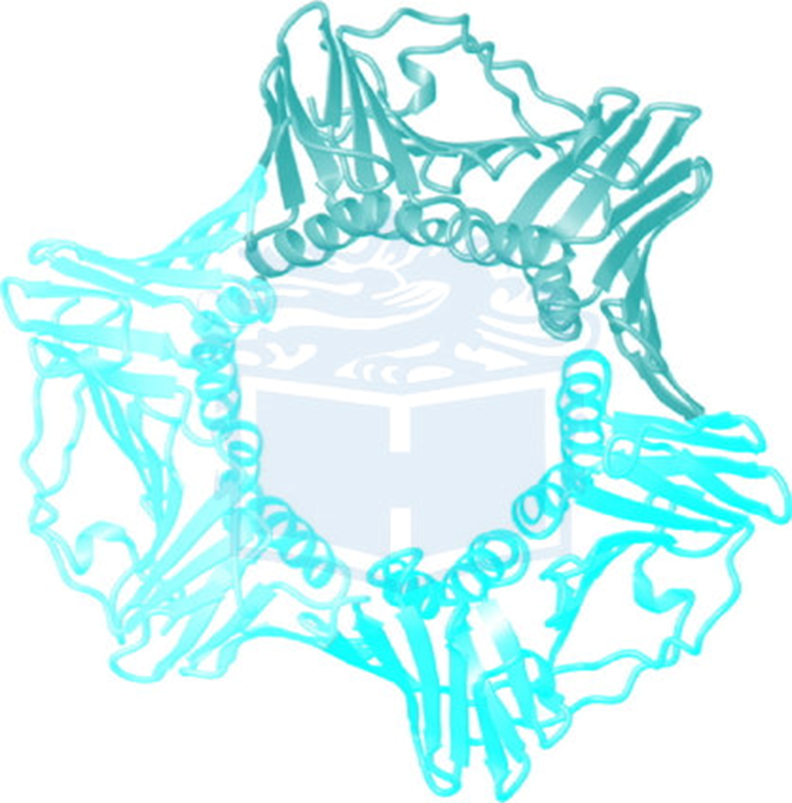
\includegraphics[width=0.5\linewidth]{PCNA滑动钳.png}
	\caption{PCNA滑动钳}
	\label{fig:pcna}
\end{figure}

DNA聚合酶$\upgamma$只存在于线粒体基质,只负责线粒体DNA复制。

\paragraph{古菌的DNA聚合酶}

古菌的DNA聚合酶有两类,一类与真核生物的$\updelta$和$\upvarepsilon$相似,也具有PCNA钳;另一类主要包括耐热的\textit{Pfu} DNA聚合酶(有校对活性)、\textit{Taq} DNA聚合酶(无校对活性)。

\subsubsection{DNA解链酶}

DNA解链酶就是催化DNA双螺旋解开的酶。任何一种DNA解链酶都可以序列无关地结合DNA。大多数解链酶优先结合DNA单链区域。

DNA解链酶具有下列酶活性:
\begin{description}
	\item[移位酶] 这使得DNA解链酶可以在DNA链这个轨道上移动(\autoref{fig:Dnab});
	\item[ATP酶] 解链需要打破氢键、碱基堆积力,这需要ATP提供能量。
\end{description}

\begin{figure}
	\centering
	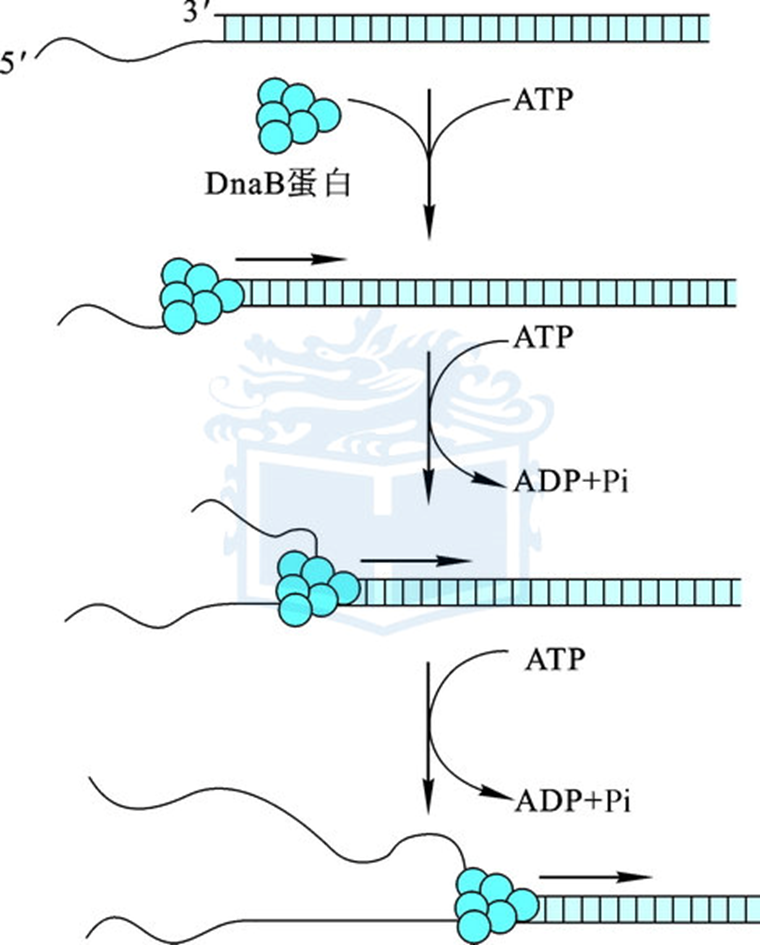
\includegraphics[width=0.5\linewidth]{Pics/DnaB}
	\caption{DnaB蛋白的移位酶活性}
	\label{fig:Dnab}
\end{figure}


在体外,我们使用热变性让DNA两条链分开,如在PCR中DNA的变性。

\subsubsection{单链结合蛋白(SSB)}

SSB专门与DNA单链区域结合,本身并没有酶活性。它具有以下功能:

\begin{itemize}
	\item 维持DNA的单链状态,防止互补碱基重新配对;
	\item 防止DNA自发形成链内双螺旋,防止DNA聚合酶进行性因链内双螺旋受到影响;
	\item 包被单链DNA区段,防止核酸酶的水解;
	\item 刺激某些酶的活性。
\end{itemize}

SSB与DNA的结合还具有协同效应,当第一个SSB与DNA结合后,后面来的SSB就会更容易与DNA结合。

利用SSB与DNA单链的特异性结合,可以设计蛋白质纯化的方法。将目的蛋白和SSB融合表达,再将含融合蛋白的细胞裂解液通过与DNA交联的树脂,融合蛋白就被吸附在树脂上,后续进行洗脱即可。

\subsubsection{DNA拓扑异构酶}

如前述,DNA形成正超螺旋时,不利于解链,也就不利于复制;形成负超螺旋时,有利于解链和复制。所以,无论真核还是原核生物,在DNA尚未复制时,都是正超螺旋;DNA复制时,就变为负超螺旋。

DNA复制时,前面的DNA解链,后面的DNA就被挤成了正超螺旋(\autoref{fig:dna_positive_supercoiling})。这时就需要DNA拓扑异构酶出手了(\autoref{fig:DNA_topoisomerase})。

\begin{figure}[h]
	\centering
	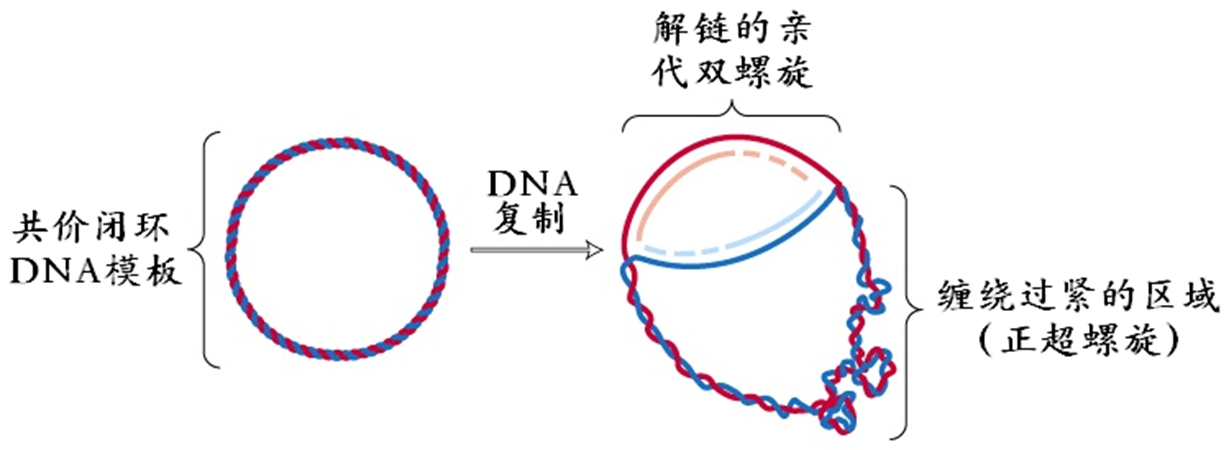
\includegraphics[width=0.7\linewidth]{Pics/DNA形成正超螺旋}
	\caption{DNA复制过程中形成的正超螺旋结构}
	\label{fig:dna_positive_supercoiling}
\end{figure}

\begin{figure}[h]
	\centering
	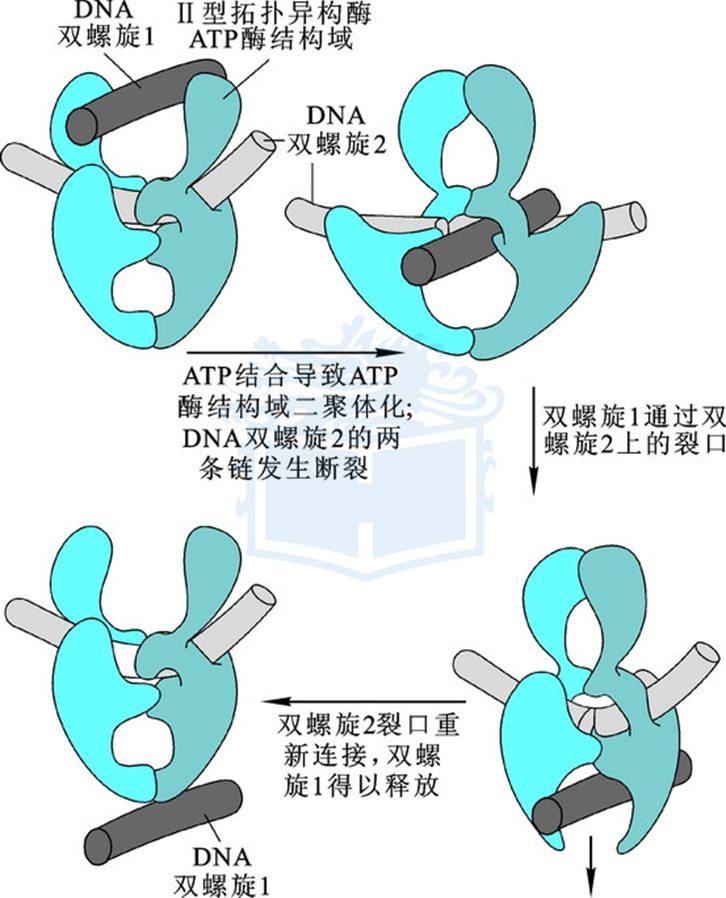
\includegraphics[width=0.7\linewidth]{Pics/DNA拓扑异构酶}
	\caption{II型DNA拓扑异构酶作用机制}
	\label{fig:DNA_topoisomerase}
\end{figure}

所有DNA拓扑异构酶的作用都是通过两次转酯反应完成的,依靠活性中心的Tyr残基。先催化DNA链断裂,移动后再催化其连接。(\autoref{fig:DNA_topoisomerase_mechanism})

\begin{figure}[h]
	\centering
	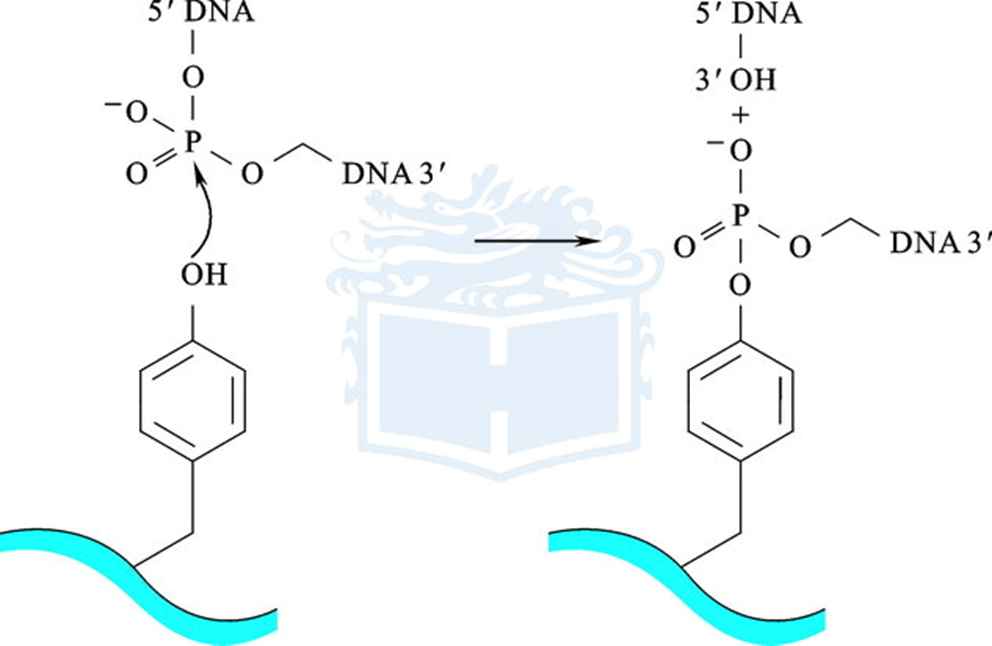
\includegraphics[width=0.7\linewidth]{Pics/DNA拓扑异构酶机理}
	\caption{DNA拓扑异构酶催化的转酯反应}
	\label{fig:DNA_topoisomerase_mechanism}
\end{figure}

DNA拓扑异构酶有不同类型,性质有所不同。I型切开一条链,II型切开两条链。参与DNA复制的主要是II类。

细菌的旋转酶就属于II类DNA拓扑异构酶,A、B亚基各2个。环丙沙星抑制A亚基,抑制ATP酶活性;新生霉素作用于B亚基,增强旋转酶切断DNA酶的能力、抑制DNA链的重新连接。

喜树碱可以抑制真核生物的DNA拓扑异构酶,可以用于治疗癌症。

\subsubsection{DNA引发酶}

DNA引发酶是特殊的RNA聚合酶,负责RNA引物的合成。由于DNA复制具有半不连续性,所以DNA引发酶在前导链上只需要引发一次,在后随链上要引发多次。

大肠杆菌的引发酶为DnaG蛋白,真核细胞的引发酶在体内和DNA聚合酶$\upalpha$紧密结合在一起。真核细胞合成的引物短一些。

\subsubsection{切除引物的酶}

RNA引物在DNA复制完之后就要被切除。

细菌切除引物的酶是DNA聚合酶I或核糖核酸酶H(RNase H)。DNA聚合酶I利用自身5$\prime$外切酶活性切除引物;RNase H专门水解和DNA杂交(Hybrid)的RNA,其中就包含RNA引物。

真核生物没有兼职切引物的DNA聚合酶。RNase H1/FEN1这两个酶配合在一起负责切除RNA引物。FEN1称为翼式内切酶,有5$\prime$外切酶和内切酶活性。一般认为,RNase H1先切除引物,但是最后剩一个,由FEN1切除。

\subsubsection{DNA连接酶}

DNA连接酶识别DNA分子内相邻的3$\prime$-羟基和5$\prime$-磷酸,并催化形成3$\prime$,5$\prime$-磷酸二酯键,其活性中心是Lys残基。有时甚至催化的是DNA分子两条链上的碱基相连。

DNA连接酶在DNA复制中,担当连接冈崎片段的任务;在DNA修复和重组中,则负责闭合DNA链上的切口。

DNA连接酶催化反应时消耗的能量来源于\ce{NAD+}或ATP。绝大多数细菌属于前者,少数细菌、所有真核生物、古菌、病毒属于后者。从\ce{NAD+}的结构就可以看出,它“相当于”一个ADP。

\subsubsection{端粒酶}

DNA每次复制,后随链上最后一个冈崎片段切除掉RNA引物后,就没有了下一次DNA复制起始,导致切掉的那一段空着了,反复下去就导致端粒\footnote{人的端粒重复序列是TTAGGG。}缩短。为了补上这一段缺失,需要端粒酶(\autoref{fig:telomere})。

\begin{figure}[h]
	\centering
	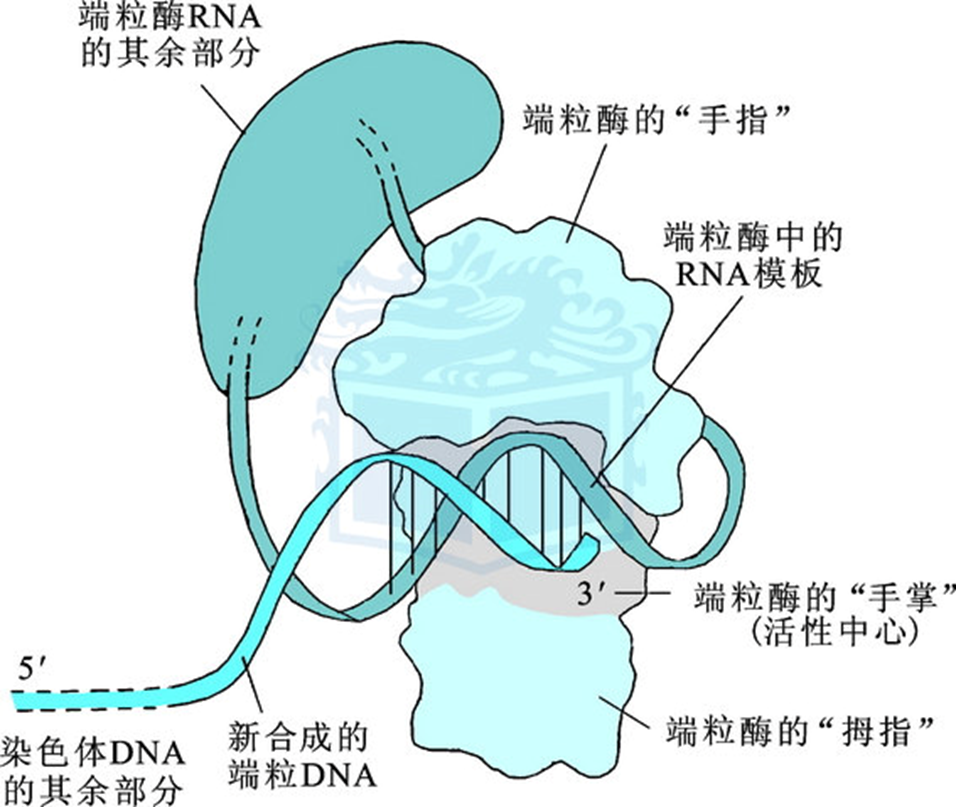
\includegraphics[width=0.5\linewidth]{Pics/端粒酶}
	\caption{端粒酶的结构}
	\label{fig:telomere}
\end{figure}


端粒酶是逆转录酶,含有蛋白质和RNA,RNA是逆转录的模板。

端粒酶作用机制见。需要注意的是,\zhongdian{端粒酶并非直接延长变短的端粒,而是先延长模板链(老链),再由DNA聚合酶把变短的端粒补上。}(\autoref{fig:telomere_mechanism})

\begin{figure}[htbp]
	\centering
	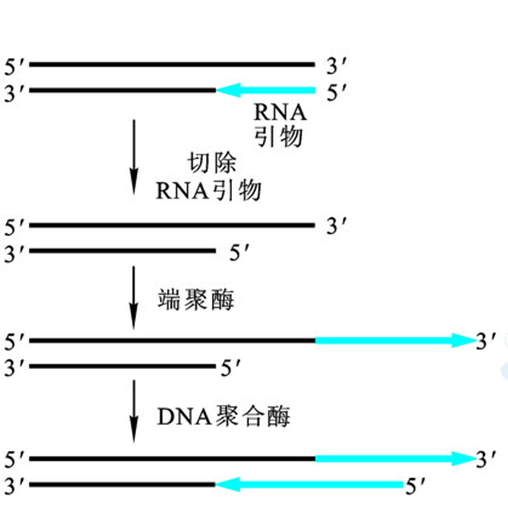
\includegraphics[width=0.4\linewidth]{Pics/端粒酶1}
	\caption{端粒酶的作用机制}
	\label{fig:telomere_mechanism}
\end{figure}

\zhongdian{多细胞生物体内大多数体细胞都没有端粒酶活性},这是为了限制分裂次数,防止DNA突变的积累。只有\zhongdian{胚胎细胞、生殖细胞、癌细胞才有端粒酶活性}。

对于\zhongdian{单细胞真核生物,其体内端粒酶活性一直很高},要不然它们早就灭绝了。

细菌、线粒体、叶绿体等\zhongdian{具有环形DNA的生物(或结构),不需要端粒酶}。

\sy{Werner综合征}的病因是端粒比正常人更快变短。

\subsection{DNA复制的详细机制}

DNA复制是以\sy{复制子}为单位进行的。任何一个复制子都含有一个复制起始区,有的还含有终止区。没有终止区不影响DNA复制的终止。

细菌、噬菌体、质粒、线粒体的基因组都只有一个复制子,真核细胞内每个染色体上的DNA都有多个复制子。

起始、延伸和终止三个阶段是人为划分的。

\subsubsection{以大肠杆菌为代表的$\uptheta$复制}

$\uptheta$复制所需的蛋白质及其功能见\autoref{tab:ecoli_DNA_duplicatipn}。

\begin{longtable}[c]{|c|l|}
	\hline
	\multicolumn{1}{|c|}{蛋白质名称} & \multicolumn{1}{c|}{功能} \\ \hline
	\endfirsthead
	%
	\multicolumn{2}{l}{\textbf{续表}} \\
	\hline
	\multicolumn{1}{|c|}{蛋白质名称} & \multicolumn{1}{c|}{功能} \\ \hline
	\endhead
	%
	DNA旋转酶 & II型拓扑异构酶,负责清除复制叉前进中的拓扑学障碍 \\ \hline
	SSB & 单链结合蛋白 \\ \hline
	DnaA蛋白 & 复制起始因子,识别复制起始区\textit{OriC} \\ \hline
	DnaB蛋白 & DNA解链酶 \\ \hline
	DnaC蛋白 & 招募DnaB蛋白到复制叉 \\ \hline
	DnaG蛋白 & DNA引发酶,引物合成 \\ \hline
	DnaT蛋白 & 辅助DnaC蛋白的作用 \\ \hline
	HU蛋白 & 类似于真核细胞的组蛋白,结合DNA并使DNA弯曲 \\ \hline
	PriA蛋白 & 引发体的装配 \\ \hline
	PriB蛋白 & 引发体的装配 \\ \hline
	PriC蛋白 & 引发体的装配 \\ \hline
	DNA聚合酶III & DNA链的延伸 \\ \hline
	DNA聚合酶I & 切除引物,填补空隙 \\ \hline
	DNA连接酶 & 缝合相邻的冈崎片段 \\ \hline
	DNA拓扑异构酶IV & 分离子代DNA \\ \hline
	Tus & 复制终止
	\\ \hline
	\caption{参与大肠杆菌DNA复制的主要蛋白质}
	\label{tab:ecoli_DNA_duplicatipn}
\end{longtable}
\paragraph{DNA复制的起始}

这一阶段起始于对\textit{oriC}的识别,结束于引发体的形成。

\textit{oriC}包含四类序列:

\begin{description}
	\item[4个9bp重复序列] DnaA蛋白识别并结合的区域。
	\item[3个富含AT的13bp重复序列] 最先解链的区域,称为DNA解链元件。
	\item[GATC甲基化位点] 其中的A发生甲基化修饰,可解除SeqA对复制起始的抑制,激活DnaA蛋白表达。
	\item[CTG序列] 引发酶识别的序列,合成引物用。CTG还散布于后随链中。
\end{description}

复制起始之前,DNA腺嘌呤甲基转移酶(Dam)被激活,使GATC中A甲基化,DnaA含量逐渐上升。

复制起始阶段的主要反应:

\begin{enumerate}
	\item 含ATP的DnaA蛋白四聚体在HU蛋白和IHF帮助下,结合到\textit{oriC}。这种结合具有协同性。HU与DNA非特异性结合,IHF与DNA的\textit{oriC}特异性结合。
	\item
\end{enumerate}





\section{DNA的损伤、修复和突变}

DNA是唯一一种在发生损伤后可以在体内能被完全修复的分子,但也并不是所有情况都可以修复。DNA发生损伤$\longrightarrow$尝试修复$\longrightarrow$修复不了就等于发生了突变,修复得了就一切正常。

\subsection{DNA的损伤}

DNA损伤分为碱基损伤和DNA链损伤。

碱基损伤可如下分类:\begin{description}
	\item[碱基脱落] $\upbeta$-N-糖苷键可以自发水解,造成碱基脱落。脱嘌呤最普遍。
	\item[碱基转换] 一种碱基变为另一种碱基。成因可以是碱基自发地脱氨基,如C$\longrightarrow$U,A$\longrightarrow$I;可以是化学诱变剂或碱基类似物。
	\item[碱基修饰] 由某些化学试剂或活性氧造成的。如:鸟嘌呤$\xrightarrow{\text{硫酸二甲酯}}$\ce{O^6}-甲基鸟嘌呤、鸟嘌呤$\xrightarrow{\text{活性氧}}$8-氧鸟嘌呤。
	\item[碱基交联] 紫外线导致DNA上相邻的嘧啶碱基形成嘧啶二聚体,尤其是TT碱基。嘧啶二聚体包括环丁烷二聚体、4-6光产物两种类型(\autoref{fig:uv_damage})。
	\begin{figure}[h!]
		\centering
		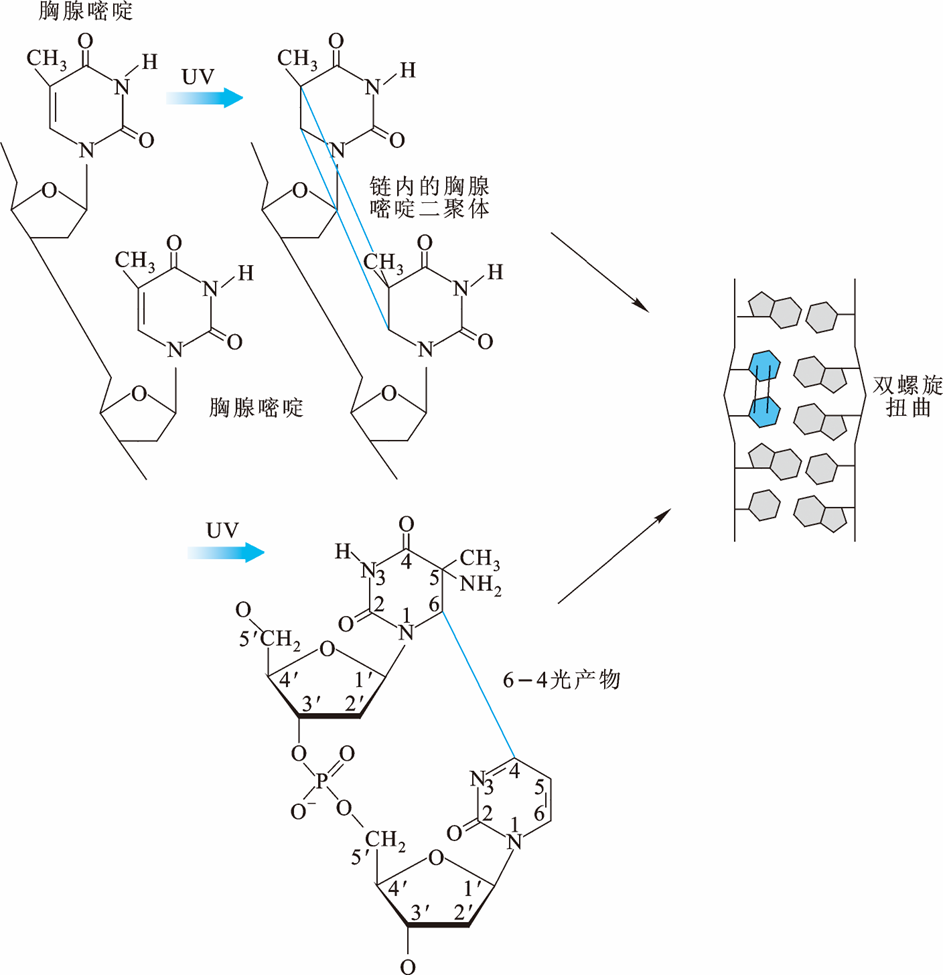
\includegraphics[width=0.7\linewidth]{4-6光产物和嘧啶二聚体}
		\caption{紫外线引发的碱基损伤}
		\label{fig:uv_damage}
	\end{figure}
	\item[碱基错配] DNA复制过程中,四种dNTP的浓度不平衡、碱基互变异构等等都有可能导致碱基错配。尽管大多数错配都会被DNA聚合酶修复,但仍然会有“漏网之鱼”。
\end{description}

DNA链损伤分为以下四类:\begin{description}
	\item[核糖核苷酸的掺入] 细胞中的NTP误入DNAP的活性中心导致。
	\item[DNA链的有断裂] 有单链断裂和双链断裂两种类型。原因有离子辐射和某些化学试剂的作用,如博来霉素。这种损伤是最严重的,当DNA链出现太多裂口,尤其是双链断裂,难以修复,就会导致细胞凋亡。
	\item[DNA链间交联] 这是由于某些双功能试剂的使用,如丝裂霉素C和顺铂。
	\item[DNA与蛋白质交联] 甲醛或较强的紫外线可诱导DNA结合蛋白与DNA之间形成共价键。
\end{description}

\subsection{DNA的修复}

DNA修复可分为直接修复、切除修复、双链断裂修复和损伤跨越。

\subsubsection{直接修复}

直接修复是将损伤的碱基或者核苷酸直接逆转,而不是切除。能够这样被修复的有:

\begin{itemize}
	\item 嘧啶二聚体;
	\item \textit{O}$^{6}$-烷基鸟嘌呤;
	\item DNA连接酶修复DNA链5'-磷酸和3'-羟基之间的断裂。
\end{itemize}

\paragraph{嘧啶二聚体的直接修复}

催化反应的酶是光裂合酶(光复活酶),分为两种:

\begin{itemize}
	\item 第一类有两个辅基: 以半醌形式存在的\ce{FAD-};5,10-甲炔基-四氢叶酸(MTHF)或8-羟基-5-去氮黄素(8-HDF)。
	\item 第二类只有一个\ce{FAD-}辅基。
\end{itemize}

对于催化修复反应来说,只有\ce{FAD-}是必须的,另外的MTHF或8-HDF能在低光条件下提高反应速率。\ce{FAD-}就相当于光系统中的中心色素,MTHF或8-HDF相当于天线色素。

大肠杆菌的光裂合酶可以结合单链或双链DNA,酶分子表面在结合DNA的地方有带正电的小孔,正好容纳嘧啶二聚体。嘧啶二聚体的出现使DNA链发生扭转、链间碱基的作用力减弱,也就使翻转过程变得容易。

\begin{wrapfigure}{r}{0.4\textwidth}
	\centering
	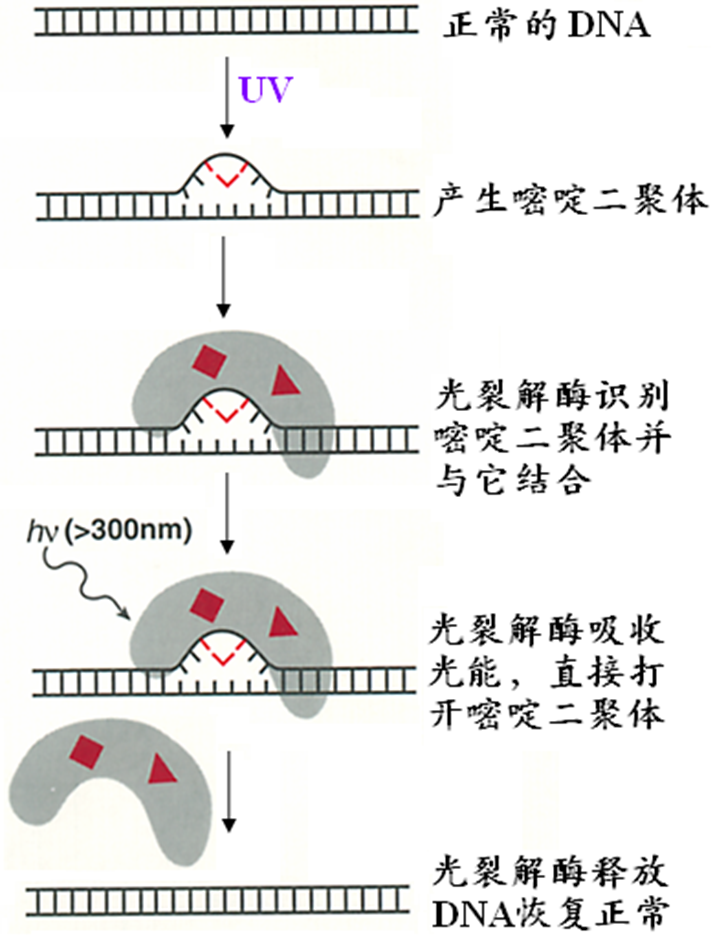
\includegraphics[width=\linewidth]{光裂合酶}
	\caption{光裂合酶的工作过程}
	\label{fig:photolyase}
\end{wrapfigure}

光裂合酶的作用过程分两步(\autoref{fig:photolyase}):\begin{enumerate}
	\item 酶直接识别、结合嘧啶二聚体,使其发生翻转落入活性中心,不需要光;
	\item 第一类光裂合酶的MTHF或8-HDF辅基吸光,把光能传给\ce{FAD-},第二类则是\ce{FAD-}直接捕获光能。\ce{FAD-}接收光能后失去一个电子,传给嘧啶二聚体,使它变得不稳定,最后二聚体之间的共价键被打破,电子又回来。\ce{FAD-}再生。
\end{enumerate}

光裂合酶广泛存在于各种生物中,但\zhongdian{胎盘类哺乳动物没有}。在这些动物体内发现了隐花色素(CRY),是光复活酶的同源蛋白,具有\ce{FAD-}和捕光色素,但没有光裂合酶的活性,可能是光信号的受体,参与生物钟的调节。

\paragraph{烷基化碱基的直接修复}

由烷基转移酶催化,以\textit{O}$^{6}$-甲基鸟嘌呤甲基转移酶(MGMT)最常见。它是“自杀式催化” 的(\autoref{fig:alkyltranseferase})。直接将碱基上的烷基转移到自己的Cys巯基上,然后失活。该酶是一种诱导酶。

\begin{wrapfigure}{r}{0.3\textwidth}
	\centering
	\includegraphics[width=\linewidth]{烷基转移酶}
	\caption{烷基化碱基的直接修复}
	\label{fig:alkyltranseferase}
\end{wrapfigure}

人体的\textit{O}$^{6}$-烷基鸟嘌呤甲基转移酶(AGT)与DNA结合的模体是HTH,但却在小沟内识别碱基序列。AGT会先通过Tyr残基,催化G的翻转落入活性中心,空缺的位置用酶的Arg残基填补。

\subsubsection{切除修复}

切除修复就是切除受损的碱基或核苷酸,然后重新合成正常的碱基或核苷酸,再经连接酶把接口缝合。整个修复过程包括识别、切除、重新合成、重新连接四步(4R)。

切除修复分为:\begin{description}
	\item[碱基切除修复(BER)] 直接识别受损伤的碱基;
	\item[核苷酸切除修复(NER)] 识别损伤对DNA双螺旋结构的扭曲,这意味着损伤更严重。
\end{description}

BER和NER的选择,就在于损伤的性质。若损伤对整个DNA链造成影响,则会采用NER。

\paragraph{碱基切除修复(BER)}

NER的过程如下:(\autoref{fig:ber})

\begin{enumerate}
	\item DNA糖苷酶沿小沟扫描,发现损伤碱基后讲起翻转,空位由Arg残基填补;
	\item DNA糖苷酶断裂碱基的$\beta$-\textit{N}-糖苷键,碱基被切除,产生无碱基位点(AP);
	\item 无碱基位点不稳定,需要被AP内切酶切断脱氧核糖之间的磷酸二酯键;
	\item 切口3$\prime$-OH可直接做引物,DNA聚合酶启动修补合成;
	\item 修补合成分为短修补和长修补,短修补为主;
	\item 短修补后产生单个暴露在外的AP位点,由磷酸二酯酶、裂合酶或外切酶切除;长修补产生游离的寡聚核苷酸,由外切酶切除。
	\item 最后DNA连接酶催化连接。
\end{enumerate}

进行短修补和长修补是由各类DNA聚合酶的相对活性决定的。如真核细胞短修补用聚合酶$\upbeta$,长修补则使用$\updelta$、$\upvarepsilon$。

\begin{figure}[htbp]
	\centering
	\includegraphics{尿嘧啶BER.png}
	\caption{尿嘧啶的切除修复}
	\label{fig:ber}
\end{figure}

\paragraph{核苷酸切除修复(NER)}

NER用于修复比较大的损伤,如嘧啶二聚体。

NER分为全局NER(GGR)和转录偶联性NER(TCR)。GGR效率低,TCR效率高。TCR的区别只是由RNA聚合酶识别损伤,其余步骤与GGR相同。

\subparagraph{细菌的NER}

大肠杆菌的GGR系统需要UvrA\textasciitilde UvrD、DNA聚合酶I/II、DNA连接酶。

修复的具体步骤:

\begin{enumerate}
	\item 形成UvrA$_{2}$UvrB三聚体,与DNA随机结合,单向移动查找碱基损伤,需要ATP;
	\item 发现损伤后,UvrA立即解离,UvrB催化损伤处DNA解链,形成预剪切复合物;
	\item UvrC被招募,先后在损伤下、上游产生切口。UvrC两次切割的过程使用不同的活性中心。该反应需要UvrB结合ATP,但不需要水解;
	\item UvrC解离,UvrD随后催化解链,将切下来的寡核苷酸片段移除;
	\item DNA聚合酶I/II将UvrB取代下来,催化修复合成;
	\item DNA连接酶缝合缺口。
\end{enumerate}

TCR系统中,RNA聚合酶发现损伤后,招募转录修复偶联因子(TRCF)。TRCF释放转录物,招募UvrA$_{2}$UvrB,促进UvrA$_{2}$解离,加快预剪切复合物形成。

\subparagraph{真核生物的NER}


\autoref{tab:原核生物和真核生物的NER比较}

\begin{table}[htbp]
	\centering
	\begin{tabularx}{\textwidth}{|c|CC|CC|}
		\hline
		\multirow{2}{*}{功能} & \multicolumn{2}{c|}{原核生物} & \multicolumn{2}{c|}{真核生物} \\ \cline{2-5}
		& \multicolumn{1}{C|}{GGR} & TCR & \multicolumn{1}{C|}{GGR} & TCR \\ \hline
		识别损伤 & \multicolumn{1}{c|}{UvrA$_{2}$UvrB} & RNA聚合酶 & \multicolumn{1}{c|}{XPC/HR23B} & RNA聚合酶 \\ \hline
		TCR招募 & \multicolumn{1}{c|}{} & TRCF & \multicolumn{1}{c|}{} & CSA、CSB \\ \hline
		解链 & \multicolumn{2}{c|}{UvrB、UvrD} & \multicolumn{2}{c|}{XPB、XPD} \\ \hline
		切除损伤 & \multicolumn{2}{c|}{UvrC} & \multicolumn{2}{c|}{XPG、XPF/ERCC1} \\ \hline
		修复合成 & \multicolumn{2}{c|}{DNA聚合酶I、II} & \multicolumn{2}{c|}{DNA聚合酶$\updelta$、 $\upvarepsilon$、PCNA} \\ \hline
		缝合切口 & \multicolumn{2}{c|}{DNA连接酶} & \multicolumn{2}{c|}{DNA连接酶I} \\ \hline
	\end{tabularx}
	\caption{原核生物和真核生物的NER比较}
	\label{tab:原核生物和真核生物的NER比较}
\end{table}

\paragraph{错配修复(MMR)}


\section{DNA重组}


\subsection{转座重组}

\begin{gs}[:“跳跃基因”的发现]
	\hspace{2em}Barbara McClintock 在20世纪30年代末期,开始了她关于遗传学的革命性研究。当时,科学界普遍认为基因是静止的,固定在染色体上的。然而,McClintock 在玉米的研究中发现了一种异常现象——某些基因能够在染色体上移动,这种现象被她称为“跳跃基因”。

	\hspace{2em}起初,这一发现并没有得到学术界的认可。许多人认为她的观察结果过于怪异,甚至怀疑她的实验数据。尽管如此,McClintock 依然坚持自己的理论,继续深入研究。她在实验中仔细记录着每一次基因移动的过程,逐渐揭示了基因并非一成不变,它们能够在染色体之间跳跃,从而影响遗传特征。

	\hspace{2em}随着时间的推移,McClintock 的理论逐渐被认可。她的发现为基因研究带来了新的视角,打破了原有的静态观念,揭示了基因的动态变化。直到20世纪50年代和60年代,学术界才开始意识到她的贡献,并逐渐给予她应有的尊重。

	\hspace{2em}最终,McClintock 在1983年因其对遗传学的杰出贡献获得了诺贝尔生理学或医学奖。这一奖项不仅是对她科学成就的肯定,也为她多年来坚持不懈的研究和探索提供了回报。她的工作为现代分子生物学的发展奠定了基础,改变了我们对基因及其功能的理解。
\end{gs}

\section{DNA转录}

细胞内主要含有的RNA有三种:mRNA、tRNA、rRNA,此外还有一些小RNA,如真核细胞内的miRNA、snRNA、7SL RNA。这些RNA都能与DNA杂交,表明它们都是转录出来的。

\subsection{DNA转录的一般特征}

DNA转录可以发生在细胞内,包括细胞质基质(原核生物、古菌)、细胞核(真核生物)、线粒体基质、叶绿体基质,也可以发生在体外。

DNA转录有以下共同特征:

\begin{enumerate}
	\item 转录有选择性和不对称性。不同于DNA复制,对于一个基因而言,只有一条DNA链作为转录模板,称模板链,而且一个基因的转录并非时刻都在进行、不同基因未必都以同一条链作模板链。

	模板链和非模板链相对,它们有一些别名:(\autoref{tab:template_strand})

	\begin{table}[h!]
		\centering
		\begin{tabular}{|c|l|c|}
			\cline{1-1} \cline{3-3}
			\textbf{模板链} & ~ & \textbf{非模板链} \\ \cline{1-1} \cline{3-3}
			非编码链 &  & 编码链 \\ \cline{1-1} \cline{3-3}
			无义链 &  & 有义链 \\ \cline{1-1} \cline{3-3}
			Waston链 &  & Crick链 \\ \cline{1-1} \cline{3-3}
		\end{tabular}
		\caption{模板链和非模板链的别名}
		\label{tab:template_strand}
	\end{table}

	\item 以四种NTPs为原料,需要2个\ce{Mg^2+}。
	\item 转录需要模板、解链,但不需要引物。
	\item 最先转录出来的通常是嘌呤碱基。
	\item 转录也有高度忠实性,但比DNA复制低。
	\item 方向和DNA复制一样,从5'$\rightleftharpoons$3'。
	\item 高度的进行性。意思是说,RNA聚合酶一旦结合,在转录终止前就不再脱落,万一酶从模板上解离,就再也不会重新结合。
	\item 转录受到严格调控。
\end{enumerate}

\subsection{RNA聚合酶}

转录起主导作用的是RNA聚合酶,全名叫依赖于DNA的RNA聚合酶。催化的反应通式为:
\[
n\text{NTPs}\xrightarrow[\text{RNA聚合酶}]{\text{DNA模板},\ce{Mg^2+}}(\text{NMP})_{n}+\text{PPi}
\]

反应机制与DNA聚合酶极为相似,再次提醒,这里生成PPi,相当于是两个ATP的能量。

这两类聚合酶仍有一些差别,下面详述:
\begin{enumerate}
	\item RNA聚合酶只有5'$\longrightarrow$3'聚合酶活性,无3'外切酶活性,这使得转录的忠实性不如DNA复制。但是RNA聚合酶具有“潜在的”内切酶活性,下面分开来讲:
	\begin{itemize}
		\item 活性中心本来就具有内切酶活性,如真核细胞的RNA聚合酶I;
		\item 与特定的转录因子结合,组装成完整的内切酶活性中心,如细菌的RNA聚合酶、真核细胞的RNA聚合酶II。
	\end{itemize}
	\item RNA聚合酶自带解链酶活性。
	\item RNA聚合酶不需要引物。
	\item 转录起始阶段,RNA聚合酶会催化几次无效转录,即RNA聚合酶在离开启动子进入转录延伸阶段之前,会反复启动转录,并释放出很短的无用转录物。
	\item 在转录起始阶段,DNA会在RNA聚合酶的活性中心形成褶皱,保证RNA聚合酶在进行无效转录时,仍能与启动子结合。
	\item 转录过程中,RNA产物不断与模板解离。
	\item RNA聚合酶在转录起始阶段受到多种调节蛋白的调控。
	\item 底物是NTP而不是dNTP。有U,无T。RNA聚合酶可以识别核糖环上的2'-OH,以此区分NTP和dNTP。
	\item 启动转录需要识别启动子。
	\item 反应速率低。
\end{enumerate}

\subsubsection{细菌的RNA聚合酶——以大肠杆菌为例}

大肠杆菌的RNA聚合酶有核心酶和全酶两种形式,核心酶的组成为$\upalpha_2\upbeta\upbeta'\upomega$,其中$\upbeta'$亚基结合有2个\ce{Mg^2+}。$\text{全酶}=\text{核心酶} + \upsigma\text{因子}$各亚基功能见\autoref{tab:ecoli_RNAP}。

\begin{table}[h]
	\centering
	\begin{tabular}{|c|c|c|c|m{15em}|}
		\hline
		\textbf{亚基} & \textbf{基因} & \textbf{分子量($\displaystyle\times 10^{3}$)} & 数目/酶 & \multicolumn{1}{c|}{\textbf{功能}} \\ \hline
		$\upalpha$ & \textit{RopA} & 36 & 2 & 核心酶的组装,转录起始,与调节蛋白的作用 \\ \hline
		$\upbeta$ & \textit{RopB} & 151 & 1 & 转录的起始和延伸 \\ \hline
		$\upbeta'$ & \textit{RopC} & 155 & 1 & 与DNA非特异性结合 \\ \hline
		$\upomega$ & \textit{RopZ} & 11 & 1 & 促进核心酶的组装,为β′亚基的分子伴侣,在体外为变性的RNA聚合酶成功复性所必需 \\ \hline
		$\upsigma_{70}$ & \textit{RopD} & 70 & 1 & 启动子的识别 \\ \hline
	\end{tabular}
	\caption{大肠杆菌RNA聚合酶的组成}
	\label{tab:ecoli_RNAP}
\end{table}


	\chapter{细胞生物学}
		\section{绪论}

\subsection{细胞大小的决定}

一般认为,细胞的大小取决于核糖体的活性,因为蛋白质的量由核糖体决定。最小的细胞是支原体。

从果蝇到哺乳动物,都应用一套几乎完全相同的信号网络来调控细胞大小。在哺乳动物中,这一网络的中心是一个名为mTOR(哺乳动物雷帕霉素靶蛋白\footnote{Mammalian target of rapamycin,因其能被雷帕霉素抑制得名。})的蛋白激酶。如果mTOR失活,细胞体积缩小。(\autoref{fig:mtor})

\begin{figure}[htbp]
	\centering
	\includegraphics[width=0.5\textwidth]{Pics/mTOR}
	\caption{调控细胞大小的信号网络}
	\label{fig:mtor}
\end{figure}

\begin{figure}[htbp]
	\centering
	\includegraphics[width=.3\textwidth]{Pics/古细菌的细胞膜}
	\caption{古细菌膜脂的醚键}
	\label{fig:archaealMembraneLipidEtherBonds}
\end{figure}

细胞的大小还与其他因素有关,如植物细胞里液泡体积增大也会使细胞体积增大。

\subsection{古细菌(古核细胞)}

通过直系同源基因相似性比较,发现古细菌和真细菌在很早就分化了。很多古细菌都生活在极端环境中。

古细菌的特点:

\begin{description}
	\item[细胞壁] 古细菌的细胞壁没有胞壁酸或肽聚糖,革兰氏染色呈阴性或阳性。
	\item[细胞质膜] 古细菌的膜脂是以醚键(\autoref{fig:archaealMembraneLipidEtherBonds})与甘油结合,膜脂中还含有鲨烯衍生物,是一种非极性脂质。
	\item[基因结构] 与细菌相似之处是:环状DNA、有操纵子、大部分无内含子、具多顺反子;与真核生物相似之处是:类似核小体的结构、部分基因有内含子、RNA聚合酶为复杂多聚体、翻译起始氨基酸是Met;
	\item[核糖体] 古核生物的核糖体与真核生物更接近,但多数古核生物核糖体是70S。抑制细菌核糖体的药物对古菌无效。
\end{description}

古核生物、原核生物、真核生物的比较见\autoref{tab:三种细胞的比较}。

\begin{table}[htbp]
\centering
\begin{tabularx}{\textwidth}{|C|c|c|c|}
	\hline
	\textbf{特征} & \textbf{原核细胞} & \textbf{古核细胞} & \textbf{真核细胞} \\ \hline
	细胞膜 & \cellcolor{blue!40}多功能 & \cellcolor{blue!40}多功能 & 功能少 \\ \hline
	核膜 & \cellcolor{blue!40}无 & \cellcolor{blue!40}无 & 有 \\ \hline
	核DNA & \cellcolor{blue!40}单个(少数多个)环状 & \cellcolor{blue!40}单个环状 & 多条线性 \\ \hline
	组蛋白 & 无或少有 & \cellcolor{red!40}有 & \cellcolor{red!40}有 \\ \hline
	核仁 & \cellcolor{blue!40}无 & \cellcolor{blue!40}无 & 有 \\ \hline
	核糖体 & \cellcolor{blue!40}70S=50S+30S & \cellcolor{blue!40}70S=50S+30S\footnotemark & 80S=60S+40S \\ \hline
	核糖体对氯霉素 & 敏感 & \cellcolor{red!40}不敏感 & \cellcolor{red!40}不敏感 \\ \hline
	翻译起始 & fMet & \cellcolor{red!40}Met & \cellcolor{red!40}Met \\ \hline
	膜质细胞器 & \cellcolor{blue!40}无 & \cellcolor{blue!40}无 & 有 \\ \hline
	质DNA & \cellcolor{blue!40}质粒 & \cellcolor{blue!40}质粒 & 线粒体,叶绿体 \\ \hline
	细胞壁 & 主要是肽聚糖 & 蛋白质 & 多样 \\ \hline
	细胞骨架 & 有 & 有 & 有 \\ \hline
	增殖方式 & \cellcolor{blue!40}无丝分裂 & \cellcolor{blue!40}无丝分裂 & 有丝分裂为主 \\ \hline
\end{tabularx}
\caption{三种细胞的比较}
\label{tab:三种细胞的比较}
\end{table}
\footnotetext{古菌的核糖体虽然与原核生物沉降系数相同,\zhongdian{但是其蛋白质组成与真核细胞更接近。}}

\section{细胞质膜}

\subsection{细胞质膜的结构}

\subsubsection{结构模型}

用锇酸固定细胞,由于锇酸与磷脂分子头部亲和力强,所以形成电镜中“暗-亮-暗”三层条带。(\autoref{fig:plasma_menb_em})

\begin{figure}[htbp]
	\centering
	\includegraphics[width=0.5\linewidth]{Pics/电镜下的细胞质膜}
	\caption{电镜下的细胞质膜}
	\label{fig:plasma_menb_em}
\end{figure}

\paragraph{流动镶嵌模型}

在三明治模型、单位膜模型的基础上,Robertson提出了流动镶嵌模型。要点有:
\begin{itemize}
	\item 膜的流动性;
	\item 膜蛋白分布的不对称性。
\end{itemize}

\paragraph{脂筏模型}

脂筏模型是对膜流动性的新理解。脂筏模型认为:在脂双层上漂浮着小船一样的胆固醇、鞘磷脂的富集区域,载着可执行特定功能的膜蛋白。

\paragraph{目前对膜结构的认识}

\begin{itemize}
	\item 磷脂双分子层构成生物膜的基本结构。脂筏中存在有助于维持脂筏稳定的蛋白。
	\item 蛋白质镶嵌或结合在脂双层中或表面,赋予生物膜各自的功能。
	\item 膜中生物大分子的互相作用限制了膜的流动性,也形成了许多特殊结构(如耳蜗微绒毛)。
	\item 膜处在不断变化之中,保证了代谢活动正常进行。
\end{itemize}

\subsubsection{膜脂}

膜脂是生物膜的基本组成成分。

\begin{table}[htbp]
	\centering
	\begin{tabularx}{\textwidth}{|C|c|c|c|c|}
		\hline
		蛋白 & 膜脂 & 化学键 & 位置 & 实例 \\ \hline
		N-Gly & 豆蔻酸 & 酰胺键 & 内侧 & Bid \\ \hline
		Cys-SH、Ser/Thr-OH & 软脂酸 & (硫)酯键 & 内侧 & PSD\footnotemark \\ \hline
		Cys-SH & 异戊二烯脂 & 硫酯键 & 内侧 & Ras \\ \hline
		C端氨基酸 & 磷酸乙醇胺、糖基化PI & 酰胺键 & 外侧 & 精卵融合 \\ \hline
	\end{tabularx}
	\caption{脂锚定膜蛋白的类型}
	\label{tab:脂锚定膜蛋白的类型}
\end{table}
\footnotetext{PSD在突触后膜调节NMDA、AMPA等受体活性,提高受体敏感性。}




\section{物质跨膜运输}

\section{细胞质基质与内膜系统}

\section{蛋白质分选与膜泡运输}

\subsection{蛋白质分选}

\subsubsection{蛋白质分选信号}

蛋白质分选信号是位于肽链N端、C端或中间的序列,指导蛋白质的去处。从空间结构上可以分为两类:

\begin{itemize}
	\item 一类为\zhongdian{连续的氨基酸序列},完成分选过程后,有些会被切除;
	\item 一类为\zhongdian{三维结构的信号斑},是在蛋白折叠完成后,表面原子按一定空间结构排布形成。形成信号斑的氨基酸残基可能在线性氨基酸序列上相距很远。\zhongdian{信号斑不被切除}(就算想切除也做不到)。
\end{itemize}

在连续的氨基酸序列中,有导肽和信号肽两类:

\begin{itemize}
	\item 信号肽是靶向内质网的,参与共翻译转运途径;
	\item 导肽(统称)是靶向线粒体、叶绿体、过氧化物酶体等的,参与翻译后转运途径。
\end{itemize}

靶向各细胞器的序列特征如\autoref{tab:靶向细胞器的蛋白质信号序列特征}所示。

\begin{table}[htbp]
	\centering
	\begin{tabularx}{\textwidth}{|c|c|c|C|}
		\hline
		靶细胞器 & 信号序列位置 & 切除 & 信号序列性质 \\ \hline
		内质网 & N 端 & 是 & 碱性氨基酸+疏水氨基酸 \\ \hline
		线粒体 & N 端 & 是 & 两亲$\upalpha$-螺旋 \\ \hline
		叶绿体 & N 端 & 是 & 没有共同基序 \\ \hline
		过氧化物酶体 & 多在 C 端 & 否 & PTS1(SKL)在C端,PTS2在N端 \\ \hline
		细胞核 & 变化的 & 否 & 含有短的富含Lys和Arg残基序列 \\ \hline
	\end{tabularx}
	\label{tab:靶向细胞器的蛋白质信号序列特征}
	\caption{靶向细胞器的蛋白质信号序列特征}
\end{table}
\subsubsection{蛋白质分选的基本类型}

\subsubsection{蛋白质向线粒体和叶绿体的分选}

\begin{figure}[htbp]
	\centering
	\includegraphics[width=\linewidth]{Pics/核基因编码的线粒体蛋白转运}
	\caption{核基因编码的线粒体蛋白转运}
	\label{fig:tim_tom}
\end{figure}

\subsection{细胞内膜泡运输}

细胞内膜泡运输需要多种转运膜泡参与,根据表面包被蛋白的不同,分为COP II包被膜泡、COP I包被膜泡、网格蛋白/接头蛋白(clathrin/AP)包被膜泡三类。




\section{线粒体和叶绿体}

\subsection{线粒体}

\subsubsection{线粒体的融合与分裂}

线粒体频繁的融合与分裂被认为是线粒体形态调控的基本方式,数目调控的基础。

频繁的线粒体融合与分裂实际上把线粒体联系成一个动态整体。植物细胞中,可见线粒体融合与分裂的偶联现象,生物学意义可能是共享遗传信息,植物中多个线粒体才共享一个DNA分子。

介导线粒体融合和分裂的两类蛋白质均是大分子GTP酶。

\paragraph{线粒体融合}

介导线粒体融合的蛋白质定位于线粒体外膜,在果蝇中是Fzo,在哺乳动物中是Mfn。虽然名字不同,但线粒体融合的分子机制高度保守。

虽然植物细胞中存在频繁的线粒体融合与分裂现象,但是基因组中并不存在\textit{Fzo}或\textit{Mfn}的同源基因。

目前没有发现线粒体融合的结构装置。

\paragraph{线粒体分裂}

在植物和动物细胞中,线粒体的分裂离不开发动蛋白。发动蛋白还介导许多膜相细胞器的融合与断裂,在膜泡运输中也发挥重要作用。

发动蛋白不像Mfn那样具有膜定位能力,需要借助Fis1和Mdv1来招募。

线粒体分裂装置则比较突出,称为线粒体分裂环,分为外环和内环。外环在线粒体外膜表面,内环在线粒体内膜之下。

\subsubsection{线粒体的超微结构}

线粒体的结构包含外膜、膜间隙、内膜和基质。外膜平展,内膜凹陷成嵴,\zhongdian{动物细胞常见规则折叠而成的“袋状嵴”,植物细胞常见不规则折叠而成的“管状嵴”}。

\begin{description}
	\item[外膜] 外膜上分布着\zhongdian{孔蛋白构成的通道,可开闭}。外膜通透性很高,离子环境几乎与细胞质基质相同。外膜的标志酶是单胺氧化酶。
	\item[膜间隙] 呼吸加强时,膜间隙可扩大。标志酶是腺苷酸激酶,催化ATP+AMP$\longrightarrow$2ADP。
	\item[内膜]
\end{description}

\section{细胞骨架}

细胞骨架,由粗到细包括:微管(MT)、中间丝(IF)、微丝(MF)。(\autoref{fig:cytoskeleton})细胞骨架与数目众多的结合蛋白的相互作用,是细胞结构与功能相统一的分子基础。

\begin{figure}[h]
	\centering
	\includegraphics[width=0.9\linewidth]{Pics/cytoskeleton}
	\caption{免疫荧光染色示微丝(A)、微管(B)、中间丝(C)在体外培养的小鼠上皮细胞内的分布,以及叠加图(D)}
	\label{fig:cytoskeleton}
\end{figure}


\subsection{微丝}

微丝又称肌动蛋白丝,存在于所有真核细胞内。

它的空间结构与功能取决于与之结合的微丝结合蛋白。在三类细胞骨架中,微丝更接近细胞的边缘。(\autoref{fig:cytoskeleton})

以下活动有微丝的参与:细胞突起(微绒毛、伪足)、胞质分裂、吞噬作用、细胞迁移、肌球蛋白运动(如肌细胞收缩)、细胞收缩、依赖肌球蛋白的物质运输等。

\begin{figure}[htbp]
	\centering
	\includegraphics[width=0.7\linewidth]{肌动蛋白和微丝}
	\caption{肌动蛋白单体和微丝}
	\label{fig:actin_microfibre}
\end{figure}

\subsubsection{微丝的组成}

微丝是两股F-actin组成的右手螺旋,具有极性,肌动蛋白单体有裂缝的一端称为负极,另一端为正极。主要成分是肌动蛋白(actin),肌动蛋白是细胞内含量最多的蛋白质之一\footnote{常用作WB的内参。}。

肌动蛋白在细胞内以球状肌动蛋白(G-actin)的单体和纤维状肌动蛋白(F-actin)的多聚体形式存在。

肌动蛋白单体的裂缝可以容纳\underline{ATP}/ADP和\ce{Ca^{2+}}/\underline{\ce{Mg^{2+}}}。肌动蛋白常是与画下划线的那个结合。

按照等电点分为$\upalpha$、$\upbeta$、$\upgamma$三种,等电点高低:$\upalpha>\upgamma>\upbeta$。

\begin{itemize}
	\item $\upalpha$-actin主要分布在肌细胞中,如心肌细胞、肠道平滑肌;
	\item $\upbeta$-actin主要分布在细胞的边缘;
	\item $\upgamma$-actin是应力纤维的组成成分。
\end{itemize}

原核生物也存在肌动蛋白的类似物,如MreB。



\subsubsection{微丝的组装过程}

通常只有结合ATP的肌动蛋白单体才参与微丝组装。微丝的组装受到胞内环境的影响:

\begin{itemize}
	\item \ce{Ca^{2+}}多,\ce{Na+}、\ce{K+}少,倾向于解聚;
	\item \ce{Mg^{2+}}、ATP、\ce{Na+}、\ce{K+}多,倾向于聚合。
\end{itemize}

肌动蛋白的组装分为下列几个步骤:

\begin{description}
	\item[成核反应] 如同DNA不能从头合成而需要引物,肌动蛋白单体不能直接从头组装。游离的G-actin与Arp2/3复合物(肌动蛋白相关蛋白)共同参与成核。
\end{description}
\section{细胞核、染色质}

\section{核糖体}

\section{细胞信号转导}

\section{细胞周期、细胞分裂}

\section{细胞增殖调控与癌细胞}





\section{细胞分化、干细胞}

\section{细胞衰老与细胞程序性死亡}

\subsection{细胞程序性死亡}

\begin{itemize}
	\item 炎症caspase:1、4、5、11、12;
	\item 凋亡起始caspase:2、8、9、10;
	\item 执行caspase:3、6、7。
\end{itemize}


\section{细胞的社会联系}

\subsection{细胞连接}

细胞连接是细胞之间、细胞与胞外基质相连接的结构。细胞连接包括下面三类:

\begin{description}
	\item[封闭连接] 将相邻上皮细胞的质膜紧紧地连接在一起,阻止小分子物质通过。如紧密连接。
	\item[锚定连接] 将细胞与相邻细胞或胞外基质连接。组分有胞内骨架、跨膜蛋白、胞外结构。
	\item[通信连接] 介导相邻细胞的物质转运或化学、电信号的传递。如间隙连接、化学突触、电突触(间隙连接)。
\end{description}

\subsubsection{封闭连接——以紧密连接为例}

关键结构是相邻细胞膜上跨膜蛋白形成的嵴线,

\subsubsection{锚定连接}

\begin{table}[htbp]
	\centering
	\begin{tabularx}{\textwidth}{|c|C|C|c|}
		\hline
		连接类型 & 骨架结构 & 跨膜蛋白 & 胞外结构 \\ \hline
		桥粒 & 中间丝 & 钙黏蛋白 & 相邻细胞 \\ \hline
		半桥粒 & 中间丝 & 整联蛋白 & 层粘连蛋白 \\ \hline
		黏着带 & 微丝 & 钙黏蛋白 & 相邻细胞 \\ \hline
		黏着斑 & 微丝 & 整联蛋白 & 胶原、纤连蛋白 \\ \hline
	\end{tabularx}
	\caption{锚定连接的类型}
	\label{tab:锚定连接的类型}
\end{table}

\subsection{细胞黏着}

\begin{table}[htbp]
	\centering
	\begin{tabularx}{\textwidth}{|c|C|C|C|c|}
		\hline
		CAM家族 & 配对 & 离子依赖 & 胞内骨架 & 细胞连接 \\ \hline
		钙黏蛋白 & 同亲 & + & 微丝、中间丝 & 黏着带、桥粒 \\ \hline
		选择素 & 异亲 & + & 微丝 & --- \\ \hline
		IgSF & 同亲 & - & --- & --- \\ \hline
		整联蛋白 & 异亲 & + & 微丝、中间丝 & 黏着斑、半桥粒 \\ \hline
	\end{tabularx}
	\caption{细胞黏着蛋白的分类}
	\label{tab:细胞黏着蛋白的分类}
\end{table}

\begin{table}[htbp]
	\centering
	\begin{tabularx}{\textwidth}{|c|C|c|}
		\hline
		名称 & 主要分布 & 参与细胞连接类型 \\ \hline
		E-钙黏蛋白 & 上皮细胞 & 黏着连接 \\ \hline
		N-钙黏蛋白 & 神经、心脏、骨骼肌及成纤维细胞 & 黏着连接、化学突触 \\ \hline
		P-钙黏蛋白 & 胎盘、表皮 & 黏着连接 \\ \hline
		VE-钙黏蛋白 & 内皮细胞 & 黏着连接 \\ \hline
	\end{tabularx}
	\caption{钙黏蛋白的分类}
	\label{tab:钙黏蛋白的分类}
\end{table}
	\chapter{微生物学}
		

\begin{landscape}
	\begin{table}[]
		\centering
		\zihao{5}
		\begin{tabular}{|c|c|c|c|c|c|}
			\hline
			编号 & 遗传物质 & 复制方式 & 转录模板 & 自带酶 & 举例 \\ \hline
			I & dsDNA & 在核内直接复制 & 自身 & 否 & AdV、HSV \\ \hline
			II & ssDNA & 合成互补链再复制 & 自身 & 否 & CPV \\ \hline
			III & dsRNA & 直接复制 & +ssRNA & RdRp & ReoV、RV \\ \hline
			IV & +ssRNA & 自编码RdRp复制 & 无需 & (RdRp) & PV、CoV \\ \hline
			V & -ssRNA & $\xrightarrow{\text{RdRp}}$+ssRNA$\xrightarrow{\text{RdRp}}$-ssRNA & -ssRNA & RdRp & IXV、RABV \\ \hline
			VI & +ssRNA & $\xrightarrow{\text{RT}}$DNA,整合$\xrightarrow{\text{DdRp}}$mRNA & 整合的DNA & RT & HIV、HTLV \\ \hline
			VII & dsDNA & $\xrightarrow{\text{DdDp}}$cccDNA$\xrightarrow{\text{RdRp}}$pgRNA$\xrightarrow{\text{RT}}$DNA & cccDNA$\xrightarrow{\text{RdRp}}$mRNA & RT & HBV \\ \hline
		\end{tabular}
		\caption{巴尔的摩病毒分类}
		\label{tab:巴尔的摩病毒分类}
	\end{table}
\end{landscape}
	\chapter{生物技术}
		\section{显微镜}

显微镜分为光学显微镜、电子显微镜、扫描隧道显微镜三种。它们三者之间除了都能放大微观结构之外,没有任何共同之处。

\begin{figure}[htbp]
	\centering
	\includegraphics[width=\linewidth]{Pics/三种显微镜的分辨率范围}
	\caption{三种显微镜的分辨率范围}
	\label{fig:threeTypesOfMicroscopesResolutionRange}
\end{figure}


\subsection{光学显微镜}

\begin{figure}[htbp]
	\centering
	\begin{forest}
		forest scheme
		[光学显微镜
		[普通光学显微镜]
		[相差显微镜、微分干涉显微镜]
		[荧光显微镜]
		[激光扫描共聚焦显微镜]
		[超高分辨率显微术]]
	\end{forest}
	\caption{光学显微镜技术的分类}
	\label{fig:opticalMicroscopyTechniquesClassification}
\end{figure}

\subsubsection{分辨率和普通光镜}

分辨率是能分辨出的距离最小的两点之间的距离。分辨率\[D=\frac{0.61\lambda}{N\cdot\sin\dfrac{\alpha}{2}}\]

其中;(\autoref{fig:opticalMicroscopeResolutionInfluencingFactors})
\begin{description}
	\item[$\lambda$] 光源的波长;
	\item[$N$] 介质折射率,空气为1,香柏油为1.5;
	\item[$\alpha$] 镜口角;
	\item[NA(数值口径,镜口率)] 全称是Numerical Aperture,即$N\cdot\sin\frac{\alpha}{2}$。
\end{description}

\begin{figure}[htbp]
	\centering
	\includegraphics[width=0.4\linewidth]{Pics/光学显微镜的分辨率影响因素}
	\caption{光学显微镜的分辨率影响因素}
	\label{fig:opticalMicroscopeResolutionInfluencingFactors}
\end{figure}

光学显微镜达到最大分辨率时,以上参数分别为:
\begin{itemize}
	\item $\alpha=\SI{140}{\degree}$;
	\item 油镜下,$N=1.5$;
	\item 可见光波长最短为\SI{400}{\nm};
\end{itemize}

计算可得普通光学显微镜最大分辨率为\SI{0.2}{\um}。

\subsubsection{相差显微镜和微分干涉显微镜}

二者的比较见\autoref{tab:相差显微镜和微分干涉显微镜的比较}。

\begin{table}[htbp]
	\centering
	\begin{tabularx}{\textwidth}{|c|C|C|}
		\hline
		& \textbf{相差} & \textbf{微分干涉} \\ \hline
		原理 & 衍射与干涉 & 干涉 \\ \hline
		特殊结构 & 环状光阑与相位板 & 起偏器与合偏器 \\ \hline
		两束光来源 & 衍射 & 棱镜 \\ \hline
		相位差主要来源 & 样品不同区域密度不同 & 厚度不同 \\ \hline
		观察结果 & 明暗反差 & 浮雕状 \\ \hline
	\end{tabularx}
	\caption{相差显微镜和微分干涉显微镜的比较}
	\label{tab:相差显微镜和微分干涉显微镜的比较}
\end{table}

\subsubsection{暗视野显微镜}

聚光镜中央有挡光片,视野背景是黑的,只允许被标本反射和衍射的光线进入物镜,物体边缘是亮的。分辨率比普通显微镜高50倍。(\autoref{fig:dkfld_mcscp})

\begin{figure}[htbp]
	\centering
	\includegraphics[width=0.4\linewidth]{Pics/暗视野显微镜}
	\caption{暗视野显微镜成像原理}
	\label{fig:dkfld_mcscp}
\end{figure}

在\autoref{fig:comparision_mcscp1}中,A图是普通光镜、B图是相差显微镜、C图是微分干涉显微镜、D图是暗视野显微镜所成的像。相差显微镜和微分干涉显微镜的成像区别是,前者边缘亮,后者有立体浮雕感。

\begin{figure}[htbp]
	\centering
	\includegraphics[width=0.8\linewidth]{Pics/显微镜成像对比}
	\caption{不同显微镜成像的对比}
	\label{fig:comparision_mcscp1}
\end{figure}

\subsubsection{荧光显微镜}

荧光显微镜的核心部件是滤光片系统和专用的物镜镜头。滤光片系统由激发滤光片和阻断滤光片组成。激发滤光片只允许特定波长的激发光通过,阻断滤光片只允许荧光染料所发出的荧光通过。(\autoref{fig:fluorescenceMicroscopeImagingPrinciple})

绿色荧光蛋白(GFP,\autoref{fig:gfp})是常用的荧光标记,只需将其与目标蛋白融合表达即可。

\begin{figure}[htbp]
	\centering
	\includegraphics[width=0.3\textwidth]{Pics/GFP}
	\caption{绿色荧光蛋白的结构}
	\label{fig:gfp}
\end{figure}

\begin{gs}[:GFP与诺贝尔奖]

	\hspace{2em}马丁·查尔菲(Martin Chalfie)、钱永健、下村修(Osamu Shimomura)三人因发现GFP获得诺贝尔奖。

	\hspace{2em}道格拉斯·普瑞舍(Douglas C. Prasher)是一名美国的分子生物学家。因为他对荧光蛋白水母素 (aequorin)克隆和测序而广为科学界所知。他早年曾将他的科研经验与成果与钱永健和马丁·查尔菲 (Martin Chalfie)分享过,但是他自己却因为无法获得足够的实验经费而不得不离开学术界。最终,他完全放弃了科学工作。2008年查尔菲与钱永健因为他们对于GFP的贡献而获得诺贝尔化学奖,而他们的研究极大程度是基于普瑞舍当年的研究成果上。由于这两名诺贝尔奖得主的努力,普瑞舍终于在钱永健的资助下于2010年6月回归学术界,目前在钱永健的实验室工作。
\end{gs}

\begin{figure}[htbp]
	\centering
	\includegraphics[width=0.4\linewidth]{Pics/荧光显微镜成像原理}
	\caption{荧光显微镜成像原理}
	\label{fig:fluorescenceMicroscopeImagingPrinciple}
\end{figure}

短波长的激发光通过激发滤光片,使样品中的荧光分子产生波长较长的荧光。荧光显微镜的暗视野提供了强反差背景,使微弱的荧光信号得以分辨。

\subsubsection{激光扫描共聚焦显微镜(LSCM)}

普通荧光显微镜下,来自不同焦平面的光线会互相干扰,导致图像模糊不清。激光扫描共聚焦显微镜相当于多安装了一套激光共焦成像系统,以激光或紫外光为光源,大大提高分辨率。共焦的意思就是,物镜和聚光镜的焦点在同一处。焦平面以外的光线就被遮挡住,因此只有来自焦平面的光线才可被观察。(\autoref{fig:LSCM},\autoref{fig:comparisonOfImagesObservedByFluorescenceMicroscopyAndLaserScanningConfocalMicroscopy})

由于观察到的画面只来自样品的一个焦平面,观察的焦平面还可以自动调整,故可以通过改变焦平面来进行“光学切片”,重构细胞的三维图像。

\begin{figure}[htbp]
	\centering
	\includegraphics[width=0.3\textwidth]{Pics/激光扫描共聚焦显微镜}
	\includegraphics[width=0.5\textwidth]{Pics/激光扫描共聚焦显微镜2}
	\caption{激光扫描共聚焦显微镜成像原理}
	\label{fig:LSCM}
\end{figure}


\begin{figure}[htbp]
	\centering
	\includegraphics[width=0.7\linewidth]{Pics/荧光显微镜和激光扫描共焦显微镜所观察图像的比较}
	\caption{荧光显微镜(A)和激光扫描共焦显微镜(B)所观察图像的比较}
	\label{fig:comparisonOfImagesObservedByFluorescenceMicroscopyAndLaserScanningConfocalMicroscopy}
\end{figure}

\subsubsection{超高分辨率显微术}

在该领域,\zhongdian{我国}科学家庄小威发明了\sy{STORM技术}。它基于单分子荧光检测,通过用光控制每次仅有少量随机离散的单个荧光分子发光,并准确定位单个荧光分子点的中心,通过多张图片叠加形成一幅超高分辨率图像。
\subsection{电子显微镜}

\subsubsection{电子显微镜的基本知识}

\paragraph{与光镜的区别}

见\autoref{tab:comparisonBetweenOpticalMicroscopeAndElectronMicroscope}。

\begin{table}[htbp]
	\centering
	\begin{tabularx}{\textwidth}{|c|c|c|c|c|C|}
		\hline
		显微镜类型 & 分辨本领 & 光源 & 透镜 & 真空 & 成像原理 \\ \hline
		光学显微镜 & \SI{0.2}{\um} & 可见光 & 玻璃 & 无需 & 吸光形成明暗反差和颜色变化 \\ \hline
		电子显微镜 & \SI{0.2}{\nm} & 电子束 & 电磁 & 真空 & 电子散射和透射形成明暗反差 \\ \hline
	\end{tabularx}
	\caption{光学显微镜和电子显微镜的对比}
	\label{tab:comparisonBetweenOpticalMicroscopeAndElectronMicroscope}
\end{table}

\paragraph{电镜的分辨率}

电子显微镜的图像不可直接观察,要通过荧光屏、感光胶片或电荷耦合器件(CCD)来成像。

电镜的分辨率和分辨本领并不是一回事。分辨本领指的是最理想情况下的分辨率,也即最大分辨率。而实际的分辨率常常受到制样技术的限制,如超薄切片样品中,分辨率约为超薄切片厚度的$\frac{1}{10}$。

人眼的分辨率约为\SI{0.2}{\mm}。用人眼分辨率除以光镜和电镜的分辨率即可得到各自的放大倍数。所以,光镜的放大倍数约为1000,电镜的放大倍数约为$10^6$。

\paragraph{电子显微镜的构造}

较为原始的电子显微镜的结构如\autoref{fig:emstrctr}所示,但是其成像原理并没有和现代的电镜有很大不同。

\begin{figure}[htbp]
	\centering
	\includegraphics[width=0.5\linewidth]{Pics/EM_strctr}
	\caption{电子显微镜的结构}
	\label{fig:emstrctr}
\end{figure}

电子显微镜由以下4部分构成:
\begin{description}
	\item[电子束照明系统] 包括电子枪和聚光镜。例如,可加热钨丝发射电子,通过高电压的阳极加速电子。
	\item[成像系统] 物镜、中间镜、投影镜等精密中空圆柱体内有磁场,使电子聚焦。
	\item[真空系统] 真空泵不断抽气,保持镜筒内真空。
	\item[记录系统] 通过荧光屏、感光胶片或CCD记录。
\end{description}

\subsubsection{主要电镜制样技术}

\paragraph{超薄切片}

电子束穿透能力有限,为获得较高分辨率就要将切片变得薄,一个切片只有40\textasciitilde\SI{50}{\nm}厚。这要求样品具有一定的韧性和刚性,所以要对样品进行包埋。为了在包埋过程中尽可能保留细微结构,需要先对样品进行固定。操作流程为:固定$\longrightarrow$包埋$\longrightarrow$切片$\longrightarrow$染色。(\autoref{fig:prcs_ultr_thn_sctn})

\begin{figure}[htbp]
	\centering
	\includegraphics[width=\linewidth]{Pics/超薄切片流程}
	\caption{超薄切片流程}
	\label{fig:prcs_ultr_thn_sctn}
\end{figure}

\begin{description}
	\item[固定] 固定是保持样品真实性的最重要环节。这要求保持样品的形态和精细结构不发生改变,甚至是免疫原性不变。常用固定剂是戊二醛和锇酸(\ce{OsO4},四氧化锇)。还可额外使用冷冻等物理方法来保存细微结构。取样要快速,以防细胞结构溶解。
	\item[包埋] 包埋介质需要有良好的机械性能,以便切片。生物样品含水多,包埋剂却是疏水的,所以在包埋之前要进行脱水。常用包埋剂是各种环氧树脂。
	\item[切片] 切片常用玻璃刀或钻石刀。切片需捞在覆盖有支持膜(如Formvar膜)的载网(铜网或镍网)上。
	\item[染色] 用重金属盐染色。锇酸染脂质,柠檬酸铅染蛋白质、乙酸双氧铀染核酸。
\end{description}

应用超薄切片技术,几乎可以观察各种细胞的超微结构。

超薄切片技术还可与放射同位素自显影、细胞化学、免疫化学和原位杂交等技术结合,在超微结构水平上完成蛋白质与核酸等组分定性、定位和半定量研究。

\begin{figure}[htbp]
	\centering
	\includegraphics[width=0.5\linewidth]{Pics/超薄切片技术显示的动物细胞超微结构}
	\caption{超薄切片技术显示的动物细胞超微结构}
	\label{fig:ultrathinSectioningTechnologyShowingUltrastructureOfAnimalCells}
\end{figure}

\paragraph{负染色技术}

\begin{figure}[htbp]
	\centering
	\includegraphics[width=0.5\linewidth]{Pics/流感病毒负染色电镜照片}
	\caption{流感病毒负染色电镜照片}
	\label{fig:influenzaVirusNegativeStainingElectronMicrograph}
\end{figure}


\paragraph{冷冻蚀刻技术}

\begin{figure}[htbp]
	\centering
	\includegraphics[width=\linewidth]{Pics/冷冻蚀刻技术示意图}
	\caption{冷冻蚀刻技术示意图}
	\label{fig:cryoFractureTechniqueSchematicDiagram}
\end{figure}

\subsection{扫描隧道显微镜(STM)}

特点:
\begin{itemize}
	\item 具有原子尺度的高分辨率;
	\item 可以在真空、大气、液体等多种环境测量;
	\item 非破坏性测量。
\end{itemize}

原子力显微镜


\section{核酸技术}

\subsection{核酸测序}

核酸测序测的是一级结构,即碱基排列顺序。

使核酸测序发生革命性变化的因素是:
\begin{itemize}
	\item 限制性内切酶(RE)的发现,能对DNA进行特异性切割;
	\item PAGE电泳技术的发展,能分辨单个核苷酸长度差异的序列。
\end{itemize}

下面介绍四代DNA测序技术。四代DNA测序技术的总结见\autoref{tab:DNA测序技术}。

\begin{table}[htbp]
	\centering
	\begin{tabularx}{\textwidth}{|c|C|c|c|c|c|c|}
		\hline
		代数 & 名称 & 准确性 & 读长 & 通量 & 扩增 & 合成 \\ \hline
		\multirow{2}{*}{第一代} & 双脱氧法(Sanger法) & \multirow{2}{*}{{\color{red}很高}} & \multirow{2}{*}{中} & \multirow{2}{*}{极低} & \multirow{5}{*}{是} & 是 \\ \cline{2-2} \cline{7-7}
		& 化学断裂法 &  &  &  &  & {\color{red}否} \\ \cline{1-5} \cline{7-7}
		\multirow{3}{*}{第二代} & 454焦磷酸 & \multirow{3}{*}{较高} & \multirow{3}{*}{短} & \multirow{3}{*}{极高} &  & \multirow{6}{*}{是} \\ \cline{2-2}
		& Illumina/Solexa &  &  &  &  &  \\ \cline{2-2}
		& SOLiD/Applied Biosystem &  &  &  &  &  \\ \cline{1-6}
		\multirow{2}{*}{第三代} & HeliScope & \multirow{4}{*}{高} & \multirow{4}{*}{长} & \multirow{2}{*}{中等} & \multirow{4}{*}{否} &  \\ \cline{2-2}
		& 单分子实时测序(PacBio SMRT) &  &  &  &  &  \\ \cline{1-2} \cline{5-5}
		\multirow{2}{*}{第四代} & 离子流 &  &  & \multirow{2}{*}{很高} &  &  \\ \cline{2-2} \cline{7-7}
		& 纳米孔(Oxford Nanopore) &  &  &  &  & {\color{red}否} \\ \hline
	\end{tabularx}
	\caption{DNA测序技术,“扩增”指需要大量样本,“合成”指边合成边测序}
	\label{tab:DNA测序技术}
\end{table}

\subsubsection{第一代测序}

\paragraph{双脱氧法}

双脱氧法也称末端终止法、Sanger法。它是最常用的第一代测序方法。具体原理见\autoref{fig:sanger_dna}。

\begin{figure}[p]
	\centering
	\includegraphics[width=0.7\linewidth]{Pics/Sanger法DNA测序}
	\caption{双脱氧法测序原理}
	\label{fig:sanger_dna}
\end{figure}

\paragraph{碱基特异性化学断裂法}

又称化学断裂法、Maxam-Gilbert法。

化学断裂法需要进行四组平行的反应:

\begin{description}
	\item[G特异性剪切] 在碱性条件下,先用硫酸二甲酯(DMS)处理,然后再使用哌啶处理;
	\item[嘌呤(A+G)碱基特异性剪切] DNA先进行酸处理,然后再加DMS;
	\item[嘧啶(C+T)碱基特异性剪切] 先用肼处理,然后用哌啶处理;
	\item[C特异性剪切] 在高盐下,先用肼处理,然后用哌啶处理;
\end{description}

进行聚丙烯酰胺凝胶电泳和放射自显影。比较G、A+G、C+T和C各个泳道,自下而上从自显影片上就可读出DNA序列。

\begin{figure}[htbp]
	\centering
	\includegraphics[width=0.3\linewidth]{Pics/化学断裂法测序}
	\caption{化学断裂法测序}
	\label{fig:MG_sequencing}
\end{figure}


\subsection{核酸分离纯化}

\subsubsection{酚-氯仿-异戊醇抽提}

细胞裂解后分离上清液,加入苯酚、氯仿、异戊醇(体积比$25:24:1$)。
\begin{itemize}
	\item 苯酚可竞争氢键,使蛋白质变性;
	\item 氯仿可以溶解苯酚等脂溶性物质,去除杂质;
	\item 异戊醇降低表面张力,消泡。
\end{itemize}

用乙醇和\ce{NaCl}沉淀DNA。
\begin{itemize}
	\item 加入\ce{Na+},可以中和DNA携带的负电荷。
\end{itemize}

75\%乙醇洗涤。

用TE buffer溶解DNA。

\subsubsection{质粒提取——SDS碱裂解法}

三个溶液:
\begin{description}
	\item[溶液I] 溶菌酶、\SI{50}{\mmol\per\L}葡萄糖、\SI{25}{\mmol\per\L} Tris pH 8.0,\SI{10}{\mmol\per\L}EDTA
	\begin{itemize}
		\item 溶菌酶溶解细胞壁;
		\item 葡萄糖维持溶液渗透压,防止DNA受机械剪切力损伤;
		\item EDTA可螯合金属离子,抑制DNase、促进溶菌酶的作用。
	\end{itemize}
	\item[溶液II] \SI{0.2}{\mmol\per\L} \ce{NaOH}、1\% SDS
	\begin{itemize}
		\item \ce{NaOH}调pH为碱性,使DNA变性;
		\item SDS使蛋白质变性。
	\end{itemize}
	\item[溶液III] \SI{50}{\mmol\per\L}醋酸钠、大量冰醋酸
	\begin{itemize}
		\item 形成缓冲体系,调pH至中性。
	\end{itemize}
\end{description}

后续使用酚仿抽提提取。

\subsubsection{RNA提取}


\subsubsection{核酸纯度检测}

使用Nanodrop分光光度计检测:
\begin{description}
	\item[A260/A230] \SI{230}{\nm}处是糖类、胍盐等杂质的吸收峰。纯净的核酸样品该值约为2.5。
	\item[A260/A280] 前者是核酸的吸收峰,后者是蛋白质的吸收峰,反映核酸被蛋白质污染的程度。纯净双链DNA约为1.8,RNA大于2。这一参数是最重要的。
\end{description}

浓度换算关系:1OD相当于\SI{50}{\ug\per\ml}的dsDNA、\SI{37}{\ug\per\ml}的ssDNA、\SI{40}{\ug\per\ml}的RNA。

\subsection{核酸电泳}

\subsubsection{基本原理}

电泳是带电颗粒在电场作用下发生定向迁移的过程。

电场中分子的迁移速率取决于分子的带电性、分子量、空间结构等。

\subsubsection{琼脂糖凝胶电泳}

\paragraph{琼脂糖凝胶的制备}

加入溴化乙锭(EB)、SYBR Green等结合DNA的试剂,便于检测。

\subsection{核酸杂交}

\subsubsection{DNA杂交——Southern Blot}


\subsubsection{RNA杂交——Western Blot}

\subsubsection{膜上印迹杂交}

\subsubsection{基因芯片}

\subsection{基因工程}

\subsubsection{分子克隆}

\subsubsection{聚合酶链式反应(PCR)}

\paragraph{PCR的反应体系}

\begin{description}
	\item[DNA模板]
	\item[DNA引物]
	\item[DNA pol]
	\item[dNTP]
	\item[\ce{Mg^{2+}}] 这是DNA聚合酶所必须的。有时加入的是\ce{Mn^{2+}}进行易错PCR,因为DNA聚合酶的校对活性依赖于\ce{Mg^{2+}}。
\end{description}

\paragraph{PCR操作流程}

预变性




\section{蛋白质技术}

\subsection{蛋白质分离纯化}

\subsection{蛋白质定量}

\subsubsection{凯氏定氮法}

蛋白质与硫酸和催化剂共热,硫酸铵与NaOH释放氨气,可测定含氮量/0.16

\subsubsection{双缩脲法}

碱性溶液中 cuso4 540nm比色 标准曲线

灵敏度较差,样品用量大。

\subsubsection{Lowry法}

福林酚显色  福林酚不是酚

660nm比色

\subsubsection{BCA法}

562nm BCA还原二价铜离子。溶液中不能含有EDTA或dtt等还原剂

\subsubsection{Bradford法}

考马斯亮蓝G-250在酸性溶液中鲜红色,与碱性氨基酸结合后蓝色。595nm

与还原剂兼容,但受去垢剂影响较大。

\subsubsection{工具——分光光度仪}

朗伯比尔光吸收定律 $A=\epsilon bc$

\subsection{蛋白质电泳}

\subsubsection{电泳准备}

竖着、

缓冲液:25mM Tris-HCl  190nMGLY
浓缩胶:偏中性,把蛋白质拉到同一条线上
分离胶:偏碱性




	\part{植物学、植物生理学}
	\chapter{植物形态解剖}
		
	\section{植物细胞}
	
	\subsection{植物细胞的形状和大小}
	
	植物细胞的形状多样,与其功能相适应。(\autoref{fig:植物细胞的多种形态})
	
	\begin{figure}[htbp]
		\centering
		\includegraphics[width=\linewidth]{Pics/植物细胞的多种形态}
		\caption{植物细胞的多种形态}
		\label{fig:植物细胞的多种形态}
	\end{figure}
	
	
	为了保持较大的相对表面积,细胞通常很小。特例有番茄、西瓜的“果肉”(细胞较大),棉的表皮毛、麻的纤维(仅前后径较长)等。
	
	\subsection{植物细胞的结构与功能}
	
	植物细胞的基本结构如\autoref{fig:植物细胞的结构划分}所示。
	
	\begin{figure}[htbp]
		\centering
		\begin{forest}
			forest scheme
			[植物细胞
				[细胞壁
					[胞间层]
					[初生壁]
					[次生壁]]
				[原生质体
					[原生质膜]
					[细胞核]
					[细胞质
						[细胞质基质]
						[细胞器(质体、液泡等)]
						[后含物(淀粉粒等)]]]]
		\end{forest}
		\caption{植物细胞的结构划分}
		\label{fig:植物细胞的结构划分}
	\end{figure}
	
	\subsubsection{细胞壁}
	
	\paragraph{细胞壁的层次}
	
	细胞壁的位置、化学成分等见\autoref{tab:细胞壁的层次}。
	
\begin{table}[htbp]
	\zihao{5}
	\centering
	\begin{tabularx}{\textwidth}{|c|c|c|C|c|}
		\hline
		\textbf{细胞壁} & \textbf{位置} & \textbf{特点} & \textbf{化学成分} & \textbf{功能} \\ \hline
		胞间层(中层) & 外 & 薄、可塑 & 果胶 & 彼此粘连 \\ \hline
		初生壁 & 中 & 薄,可塑 & 纤维素、半纤维素、果胶、结构蛋白 & 支持、保护 \\ \hline
		次生壁 & 内 & 厚、坚硬 & 半纤维素、纤维素、木质素 & 支持、保护 \\ \hline
	\end{tabularx}
	\caption{细胞壁的层次}
	\label{tab:细胞壁的层次}
\end{table}
	
	细胞壁中含有的物质如下列:
	\begin{description}
		\item[纤维素] 多糖,Glc残基以$\beta$-1,4糖苷键连接,组成微纤丝、大纤丝;
		\item[半纤维素] 支链与纤维素不同,按照支链的不同可分为双子叶植物中的\sy{木葡聚糖}和单子叶植物中的\sy{阿拉伯木聚糖};
		\item[胼胝质] Glc残基以$\beta$-1,3糖苷键连接的多糖,能应对机械损伤和病虫害。可由间苯二酚蓝显色;
		\item[果胶] 双子叶植物多,单子叶植物很少;
		\item[木质素] 疏水的酚醛聚合物(非糖类)。可被盐酸-间苯三酚染色。
		\item[蛋白质] 主要是结构蛋白和酶。结构蛋白包括富含羟脯氨酸、脯氨酸、甘氨酸的三类。其中富含羟脯氨酸的蛋白就是伸展蛋白。
	\end{description}
	
	除此之外,细胞壁中还随功能不同,含有角质、栓质、矿质等。
	
	细胞壁的结构单位是\sy{微纤丝}。微纤丝是一种纤维素的构架,层次有:
	\begin{center}
		葡萄糖$\longrightarrow$葡萄糖长链$\longrightarrow$微团$\longrightarrow$微纤丝$\longrightarrow$大纤丝(光镜下可见)
	\end{center}
	
	初生壁的微纤丝排列成网状,三层次生壁中微纤丝排列各不相同。细胞壁的其他物质就填充在微纤丝骨架中。
	
	初生壁中,三类物质的作用分别是:
	\begin{description}
		\item[果胶] 构成基质,如同水泥;
		\item[纤维素] 构成支持部分,如同钢筋;
		\item[半纤维素] 靠氢键交联果胶和纤维素。
	\end{description}
	
	次生壁中,需要注意:
	\begin{itemize}
		\item 并非所有细胞都有次生壁;
		\item 次生壁的3层结构中,微纤丝排列方向不同是纤维素合成酶的排列方向由微管排列方向决定的缘故;(\autoref{fig:植物细胞壁的不同层次和微纤丝的排列方向})
		\item 大多数具有次生壁的细胞均死亡。
	\end{itemize}
	
	\begin{figure}[htbp]
		\centering
		\includegraphics[width=0.4\linewidth]{Pics/次生壁的3层}
		\caption{植物细胞壁的不同层次和微纤丝的排列方向}
		\label{fig:植物细胞壁的不同层次和微纤丝的排列方向}
	\end{figure}
	
	\subsubsection{初生纹孔场与胞间连丝}
	
	初生壁上细胞壁较薄的区域称为初生纹孔场,这里分布许多小孔,有胞间连丝穿过。
	
	胞间连丝是沟通相邻细胞的原生质细丝,外有内质网形成的管道。胞间连丝并不局限于初生纹孔场。
	
	\subsubsection{纹孔}
	
	\sy{纹孔}是初生壁上没有被次生壁覆盖的部分。按照次生壁在此处的加厚特点,分为单纹孔\footnote{这里的“单”指的是简单(simple),意思是结构比较简单的一种纹孔。}和具缘纹孔。(\autoref{fig:纹孔})
	
	\begin{itemize}
		\item 具缘纹孔与单纹孔的区别就是具缘纹孔的次生壁向细胞内拱起,使纹孔腔变大。
		\item 某些裸子植物的具缘纹孔还具有纹孔塞,可控制水流。
	\end{itemize}
	
	\begin{figure}[htbp]
		\centering
		\includegraphics[width=\linewidth]{Pics/纹孔}
		\caption{纹孔}
		\label{fig:纹孔}
	\end{figure}
	
	\subsubsection{液泡}
	
	液泡由高尔基体起源。随着细胞成熟,液泡从小而分散变为大而集中。
	
	液泡内有细胞液,起到储存、防御、膨压、消化的作用。
	
	液泡可吞噬衰老细胞器,起到动物的溶酶体的功能。这一功能是由液泡膜整合蛋白(TIP)决定的。若TIP为$\gamma$型,则该液泡承担溶酶体的功能。
	
	液泡压缩了原生质的体积,相当于节省了氮元素。
	
	\subsubsection{质体}
	
	质体是植物细胞特有的细胞器之一,与糖类的合成与贮藏密切相关。
	
	按照含有色素的种类,分为:
	\begin{description}
		\item[叶绿体] 含有叶绿素、叶黄素、类胡萝卜素。进行光合作用。基质内有基粒。
		\item[有色体] 含有胡萝卜素、叶黄素。存在于果实、花瓣中。聚积淀粉和脂质,吸引传粉、传种动物。无基粒。
		\item[白色体] 不含色素。储存淀粉(淀粉体)、脂肪(造油体)。无基粒。
	\end{description}
	
	
	质体都由前质体发育而来,具体转变如\autoref{fig:质体的转化}所示。
	
	\begin{figure}[htbp]
		\centering
		\includegraphics{质体的转化}
		\caption{质体的转化}
		\label{fig:质体的转化}
	\end{figure}
	
	三种成熟质体可以互相转化,除了叶绿体不能转化为白色体。
	
	\sy{黄化质体}中含有原片层小体,是管状的膜系统,见光之后迅速发育为叶绿体的类囊体。
	
	\subsubsection{微体}
	
	微体与溶酶体相似,区别是二者含有的酶不同。溶酶体含有水解酶类,微体含有氧化酶和过氧化氢酶。
	
	微体分为过氧化物酶体和乙醛酸循环体。动物没有乙醛酸循环体。
	
	\subsection{植物细胞的后含物}

	 后含物是细胞原生质体新陈代谢产物,包含贮藏物和废物,化学上包括糖类、蛋白质、脂质、无机盐和其他有机物。后含物存在于原生质体或细胞壁。
	 
	 下面介绍常见的后含物,包括淀粉、蛋白质、脂肪、晶体。
	 
	 \subsubsection{淀粉}
	 
	 淀粉主要以\sy{淀粉粒}的形式存在。
	 
	 \begin{itemize}
	 	\item 合成过程:
	 	\begin{itemize}
	 		\item 由质体合成,白色体特化为造粉体;
	 		\item 沉积方式:由脐点逐层向外沉积;
 			\item 脐点位置决定类型:同心淀粉、离心淀粉。
	 	\end{itemize}
	 	\item 结构特征:
	 	\begin{itemize}
	 		\item 轮纹结构:直链淀粉与支链淀粉交替沉积;
	 		\item 光学差异:直链淀粉亲水性更强。
	 	\end{itemize}
	 	\item 形态分类(\autoref{fig:淀粉粒的类型}):
	 	\begin{itemize}
	 		\item 单粒淀粉粒:单脐点+同心轮纹;
	 		\item 复粒淀粉粒:多脐点+独立轮纹;
	 		\item 半复粒淀粉粒:多脐点+共同外围轮纹。
	 	\end{itemize}
	 \end{itemize}
	 
	 \begin{figure}
	 	\centering
	 	\includegraphics[width=0.3\linewidth]{Pics/淀粉粒的类型}
	 	\caption{淀粉粒的类型}
	 	\label{fig:淀粉粒的类型}
	 \end{figure}
	 
	 \subsubsection{蛋白质}
	 \begin{itemize}
	 	\item 贮藏形式:
	 	\begin{itemize}
	 		\item 蛋白质拟晶体:方形(如马铃薯块茎细胞)
	 		\item 糊粉粒:
	 		\begin{itemize}
	 			\item 结构:膜包裹的球状颗粒;
	 			\item 组成:无定形蛋白(+拟晶体),蓖麻种子的还含磷酸盐球形体(\autoref{fig:蓖麻的糊粉粒});
	 			\item 分布:胚乳糊粉层(豆类子叶细胞典型)
	 		\end{itemize}
	 		
	 		\begin{figure}[htbp]
	 			\centering
	 			\includegraphics[width=0.5\linewidth]{Pics/蓖麻的磷酸盐球形体}
	 			\caption{蓖麻的糊粉粒}
	 			\label{fig:蓖麻的糊粉粒}
	 		\end{figure}
	 		
	 	\end{itemize}
	 	\item 动态变化:
	 	\begin{itemize}
	 		\item 形成:液泡分裂$\longrightarrow$蛋白沉积$\longrightarrow$形成糊粉粒;
	 		\item 利用:糊粉粒分解$\longrightarrow$液泡重组。
	 	\end{itemize}
	 \end{itemize}
	 
	 \subsubsection{脂肪和油类}
		基本特征:
	 	\begin{itemize}
	 		\item 高能贮藏物质,体积最小
	 		\item 物理状态区分:常温固态为脂肪,液态为油类
	 	\end{itemize}
	 	
	 	质体和圆球体都能积累脂质,成为油滴。
	 
	 \subsubsection{晶体}
	 
	 \begin{itemize}
	 	\item 基本特征:
	 	\begin{itemize}
	 		\item 无机盐结晶,主要存在于液泡
	 		\item 草酸钙晶体为主
	 		\item 意义:降低次生代谢物毒性
	 		\item 特殊类型:碳酸钙晶体(钟乳体)
	 	\end{itemize}
	 	\item 形态分类(\autoref{fig:晶体的类型}):
	 	\begin{itemize}
	 		\item 单晶:棱柱状/锥状
	 		\item 针晶:针状聚集体
	 		\item 簇晶:球状复式结构
	 	\end{itemize}
	 	
	 	\begin{figure}[htbp]
	 		\centering
	 		\includegraphics[width=0.5\linewidth]{Pics/晶体的类型}
	 		\caption{晶体的类型}
	 		\label{fig:晶体的类型}
	 	\end{figure}
	 \end{itemize}
	 
	\section{植物的组织}
	
	\begin{figure}[htbp]
	\centering
	\begin{forest}
		forest scheme
		[植物组织
		[分生组织
		[按来源分
		[原分生组织]
		[初生分生组织]
		[次生分生组织]]
		[按位置分
		[顶端分生组织]
		[侧生分生组织]
		[居间分生组织]]]
		[成熟组织
		[保护组织]
		[薄壁组织]
		[机械组织]
		[输导组织]
		[分泌组织]]]
	\end{forest}
	\caption{植物的组织分类}
	\label{fig:植物的组织分类}
	\end{figure}
	
	\subsection{分生组织}
	
	如\autoref{fig:植物的组织分类}所示,分生组织可按两种不同的方式区分,而这两种方式是互相重叠的:(\autoref{fig:分生组织的分类})
	
	\begin{figure}[htbp]
		\centering
		\includegraphics{分生组织的分类}
		\caption{分生组织的分类}
		\label{fig:分生组织的分类}
	\end{figure}
	
	\begin{description}
		\item[顶端分生组织] 细胞小,核大,原生质浓厚,液泡小而分散。位于根和茎的顶端。
		\item[居间分生组织] 夹在出现了分化的组织之间的分生组织,是顶端分生组织在局部的残留。
		\item[侧生分生组织] 位于根和茎的外周,包括(维管)形成层和木栓形成层。草本双子叶植物几乎无侧生分生组织。需要注意,束中形成层是初生性质的。
		\item[原分生组织] 从胚细胞保留,完全未分化。
		\item[初生分生组织] 从原分生组织发育而来,已经开始分化。
		\item[次生分生组织] 从成熟组织脱分化而来。
	\end{description}
	
	\subsection{成熟组织}
	
	成熟组织有较大分化,在一定情况下也可脱分化产生次生分生组织。
	
	\subsubsection{保护组织}
	
	保护组织包括表皮和周皮,覆盖在植物体表面,负责保水、控制气体交换、防御。
	
	\begin{description}
		\item[表皮] 初生结构,通常为单层细胞,排列紧密,外有角质。表皮上还有表皮毛,有的有分泌功能。
		\item[周皮] 次生结构,取代表皮。由木栓形成层向外产生木栓层,向内产生栓内层。三者合称周皮。只有木栓层是死细胞。
		
		木栓形成层还可形成皮孔,是次生通气结构。
	\end{description}
	
	\subsubsection{薄壁组织}
	
	分布在各个器官中,功能十分多样。细胞壁通常较薄,只有初生壁。分化较少,有潜在的分裂能力。
	
	薄壁组织可分为多种类型:(\autoref{fig:薄壁组织的类型})
	
	\begin{figure}[htbp]
		\centering
		\includegraphics[width=\linewidth]{Pics/薄壁组织的类型}
		\caption{薄壁组织的类型}
		\label{fig:薄壁组织的类型}
	\end{figure}
	
	\subsubsection{机械组织}
	
	机械组织对细胞起主要支持作用。可分为厚壁组织和厚角组织。
	
	\begin{description}
		\item[厚角组织] 细胞壁在角隅处有初生壁性质的加厚。通常为活细胞。(\autoref{fig:南瓜茎横切示皮层厚角组织})
		
		\begin{figure}[htbp]
			\centering
			\includegraphics[width=0.5\linewidth]{Pics/南瓜茎横切示皮层厚角组织}
			\caption{南瓜茎横切示皮层厚角组织}
			\label{fig:南瓜茎横切示皮层厚角组织}
		\end{figure}
		
		\item[厚壁组织] 细胞壁次生壁性质的加厚。成熟后为死细胞。根据形态又可分为石细胞和纤维。(\autoref{fig:厚壁组织})
		
		\begin{figure}[htbp]
			\centering
			\begin{subfigure}{0.45\textwidth}
				\includegraphics[width=\linewidth]{不同形状的石细胞
				}
				\caption{石细胞}
			\end{subfigure}
			\hfill
			\begin{subfigure}{0.45\textwidth}
				\includegraphics[width=\linewidth]{纤维细胞}
				\caption{纤维细胞}
			\end{subfigure}
			\caption{厚壁组织}
			\label{fig:厚壁组织}
		\end{figure}
	\end{description}
	
	\subsubsection{输导组织}

	输导组织是植物体中负担物质长途运输的主要组织。其中,木质部的导管运输水分和无机盐,韧皮部的筛管和伴胞运输有机物。
	
	输导组织从蕨类开始出现。
	
	\paragraph{木质部}
	
	由导管分子、管胞分子、木纤维、木薄壁细胞四种不同类型细胞构成。(\autoref{tab:管胞和导管的比较})
	
	\begin{table}[htbp]
		\centering
		\begin{tabularx}{\textwidth}{|c|C|c|}
			\hline
			特点 & 管胞 & 导管 \\ \hline
			细胞结构 & 单个细胞,端部细胞壁不溶解 & 发育时端壁溶解形成穿孔 \\ \hline
			连接方式 & 纹孔及未木质化增厚部分 & 通过穿孔直接沟通 \\ \hline
			输水效率 & 较低 & 较高 \\ \hline
			存在植物 & 蕨类植物和裸子植物 & 被子植物(除最原始类群) \\ \hline
			功能 & 兼具支持和输导 & 专营输导功能 \\ \hline
			演化方向 & 系统上,分化为木纤维或导管分子 & 由管胞演化而来 \\ \hline
		\end{tabularx}
		\caption{管胞和导管的比较}
		\label{tab:管胞和导管的比较}
	\end{table}
	
	\begin{figure}[htbp]
		\centering
		\begin{subfigure}{0.6\textwidth}
			\includegraphics[width=\linewidth]{管胞}
			\caption{管胞}
		\end{subfigure}

		\begin{subfigure}{0.45\textwidth}
			\includegraphics[width=\linewidth]{导管}
			\caption{导管}
		\end{subfigure}
		\caption{管胞和导管}
		\label{fig:管胞和导管}
	\end{figure}
	
	木纤维起到加强支持的作用,细胞可死可活。木薄壁细胞具有贮藏功能,发育后期细胞壁也常常木质化。
	
	\subsubsection{韧皮部}
	
	由筛管分子、伴胞、韧皮纤维、韧皮薄壁细胞,四种不同类型细胞构成。
	
	\begin{description}
		\item[筛胞] 端壁不形成筛板,仅通过侧壁上的筛域进行运输。仅存在于裸子植物和蕨类中,有类似伴胞的细胞存在。
		\item[筛管] 活细胞,但仅保留线粒体、内质网、P蛋白体等细胞器。端壁形成筛板,原生质联络索穿过筛板连接相邻细胞。衰老或休眠的筛管,由胼胝质将其封闭。
		\item[伴胞] 伴胞和筛管起源于同一个原始细胞,是完整的细胞。有的植物的伴胞具有传递细胞的特性。
	\end{description}
	
	\subsubsection{分泌结构}
	
	根据分泌物的去向,分为内部的分泌结构和外部的分泌结构两类。
	
	\begin{description}
		\item[外分泌结构] 分泌物排出体外,如蜜腺、腺毛、排水器。
		\item[内分泌结构] 不排出体外,如分泌腔、分泌道、乳汁管。
	\end{description}
	
	分泌腔和分泌道有溶生型、裂生型和裂溶生型。显微镜下可见溶生型的具有破损的细胞。
	
	\begin{figure}[htbp]
		\centering
		\begin{subfigure}{0.45\textwidth}
			\includegraphics[width=\linewidth]{溶生型分泌腔}
			\caption{橘果皮的溶生型分泌腔}
		\end{subfigure}
		\hfill
		\begin{subfigure}{0.45\textwidth}
			\includegraphics[width=\linewidth]{裂生型分泌腔}
			\caption{漆树的裂生型分泌腔}
		\end{subfigure}
		\caption{两类分泌腔}
		\label{fig:两种不同的分泌腔}
	\end{figure}
	
	\subsubsection{组织系统}
	
	植物体或植物器官中的各类执行相同生理功能的组织,在不同的部位彼此联通,形成了组织系统。
	
	组织系统分为皮组织系统、维管组织系统和基本组织系统三类。
	
	\begin{description}
		\item[皮组织系统] 包括表皮和周皮,形成连续的保护层。
		\item[维管组织系统] 包括韧皮部和木质部,连接植物各个部分。
		\item[基本组织系统] 各类薄壁组织、厚角组织、厚壁组织。
	\end{description}
\section{植物的营养器官}
	
	
	\begin{forest}
		%forest scheme
		[营养器官
		[根]
		[茎]
		[叶]]
	\end{forest}
	
	\subsection{根}
	
	\begin{figure}
		\centering
		\begin{forest}
			forest scheme
			[根
			[按位置分
			[主根]
			[侧根]
			[不定根]]
			[结构
			[表皮]
			[外皮层]
			[内皮层]
			[中柱鞘]
			[维管柱(中柱)]]
			[变态
			[贮藏根
			[肉质直根]
			[块根]]
			[气生根
			[支柱根]
			[攀缘根]
			[呼吸根]
			[寄生根]]]]
		\end{forest}
	\end{figure}
	
	除气生根外,根是植物地下部分的营养器官。
	
	功能:吸收、固着和支持、输导、合成、贮藏和繁殖、分泌
	
	直根系、须根系
	
	\subsubsection{皮层}
	
	外皮层:排列相对紧密,在表皮破坏后代替表皮起保护作用。
	
	内皮层:最内层紧密排列,有凯氏带,是上下、径向细胞壁木质化、栓质化加厚。
	
	\subsubsection{维管柱(中柱)}
	
	中柱鞘
	
	初生木质部 外始式(向心发育) 木质部脊 n原型
	
	初生韧皮部 外始式 
	
	\subsubsection{侧根}
	
	中柱鞘细胞脱分化形成次生分生组织,形成侧根原基。内起源。
	
	\subsubsection{根的次生生长}
	
	裸子植物和木本双子叶植物有次生生长的根。
	
	\subsubsection{根的变态}
	
	\subsubsection{根的共生结构}
	
	根瘤
	
	菌根
	
	\subsection{茎}
	
	茎由胚芽或胚芽和部分下胚轴发育而成。茎内含木质成分较少的为草本植物,木质化程度高的为木本植物。
	
	功能:输导、支持、贮藏和繁殖、光合
	
	\subsubsection{茎的变态}
	
	地上部分:叶卷须、茎卷须、枝刺、肉质茎;
	
	地下部分:根状茎、块茎、球茎、鳞茎。
	
	
	\subsection{叶}
	
	\subsubsection{叶的发育}
	
	叶片是叶原基经过顶端生长、边缘生长、居间生长发育来的。
	
	
	
	\section{植物的繁殖器官}

\begin{figure}[h]
	\centering
	\includegraphics{Pics/ABCDE模型.pdf}
	\caption[ABCDE模型]{ABCDE模型}
	\label{fig:abcde}
\end{figure}

	\chapter{植物分类学}
		\section{植物分类系统}

\subsection{植物的分类}

植物分类如\autoref{tab:clsfctn_vegetbls}所示。

\begin{table}[htbp]
	\centering
	\begin{NiceTabularX}{\textwidth}{cCCC}[hvlines]
		裸藻门 & \Block[v-center]{9-1}{藻类植物} & \Block[v-center]{13-1}{孢子植物} & \Block[v-center]{11-1}{低等植物} \\
		绿藻门 &  &  &  \\
		黄藻门 &  &  &  \\
		硅藻门 &  &  &  \\
		金藻门 &  &  &  \\
		甲藻门 &  &  &  \\
		褐藻门 &  &  &  \\
		红藻门 &  &  &  \\
		蓝藻门 &  &  &  \\
		黏菌门 & \Block[v-center]{2-1}{菌类} &  &  \\
		地衣门 &  &  &  \\
		苔藓植物门 & \Block[v-center]{2-1}{颈卵器植物} &  & \Block[v-center]{4-1}{高等植物} \\
		蕨类植物门 &  &  &  \\
		裸子植物门 & \Block[v-center]{2-1}{维管植物} & \Block[v-center]{2-1}{种子植物} &  \\
		被子植物门 &  &  & 
	\end{NiceTabularX}
	\caption{植物的分类}
	\label{tab:clsfctn_vegetbls}
\end{table}

\subsection{植物分类的阶层、双名法}

植物分类的各阶层见\autoref{tab:plant_class}。

\begin{table}[htbp]
	\centering
	\begin{tabularx}{\textwidth}{|C|C|C|c|}
		\hline
		中文 & 英文 & 拉丁文 & 词尾 \\ \hline
		植物界 & Vegetable Kingdom & Regnum Vegetabile &  \\ \hline
		门 & Division & Divisio, Phylum & -phyta \\ \hline
		亚门 & Subdivision & Subdivisio & -phytina \\ \hline
		纲 & Class & Classis & -eae, -opsida \\ \hline
		亚纲 & Subclass & Subclassis & -idae \\ \hline
		目 & Order & Ordo & -ales \\ \hline
		亚目 & Suborder & Subordo & -ineae \\ \hline
		科 & Family & Familia & -aceae \\ \hline
		亚科 & Subfamily & Subfamilia & -oideae \\ \hline
		族 & Tribe & Tribus & -eae \\ \hline
		亚族 & Subtribe & Subtribus & -inae \\ \hline
		属 & Genus & Genus & -a, -um, -us \\ \hline
		亚属 & Subgenus & Subgenus &  \\ \hline
		组 & Section & Sectio &  \\ \hline
		亚组 & Subsection & Subsectio &  \\ \hline
		系 & Series & Series &  \\ \hline
		亚系 & Subseries & Subseries &  \\ \hline
		种 & Species & Species &  \\ \hline
		亚种 & Subspecies & Subspecies &  \\ \hline
		变种 & Variety & Varietas &  \\ \hline
		亚变种 & Subvariety & Subvarietas &  \\ \hline
		变型 & Form & Forma &  \\ \hline
		亚变型 & Subform & Subforma &  \\ \hline
	\end{tabularx}
	\caption{植物各阶分类单元}
	\label{tab:plant_class}
\end{table}

植物命名采用双名法。学名=属名+种加词(+命名人)。属名和种加词都要用拉丁语或拉丁化的词来写。

命名人的书写有下列要点:
\begin{itemize}
	\item 命名人通常以其姓氏的缩写来表示,还要拉丁化。林奈(Linnaeus)的缩写为L.,单字母缩写仅限林奈一人。
	\item 当子女和父母均为命名人时,子女的姓氏缩写后加“f.”或“fil.”表示子女。
	\item 二人共同命名植物时,两人姓氏缩写中间加“et.”,意为“和”;多人命名,则在第一个人的姓氏缩写后加“et al.”或“etc.”。
	\item 如一学名由甲学者提出,但未经正式发表,又由乙学者正式发表,则把甲的姓氏放前面,用“ex”(从)连接乙的姓氏。
\end{itemize}

对于亚种或变种,应用三名法或四名法,即比双名法多了亚种和变种加词。

\begin{table}[htbp]
	\centering
	\begin{tabularx}{\textwidth}{|C|C||C|C|}
		\hline
		\textbf{缩写字} & \textbf{中文} & \textbf{缩写字} & \textbf{中文} \\ \hline
		comb. nov. & 新组合 & nov. sp. & 新种 \\ \hline
		cult. & 栽培的 & sect. & 组、节 \\ \hline
		cv. & 栽培变种,品种 & sp. nov. & 新种 \\ \hline
		et & 和、同、以及 & spp. & 许多种 \\ \hline
		ex & 从、出自 & subsp. 或 ssp. & 亚种 \\ \hline
		f. & 变型 & subgen. & 亚属 \\ \hline
		nom. nud. & 裸名 & syn. & 异名 \\ \hline
		var. & 变种 &  &  \\ \hline
	\end{tabularx}
	\caption{常见拉丁文缩写}
	\label{tab:latin_abbrs}
\end{table}

\subsection{国际植物命名法规}

国际植物命名法规(巴黎法规)的要点如下:
\begin{description}
	\item[模式标本] 种和种以下的分类群的命名必须有模式标本做根据。模式标本必须永久保存,所以不能是活植物。
	\item[唯一合法学名] 每一种植物只有一个合法的学名,其他名称应作为异名或废弃。
	\item[学名的格式] 学名包括属名和种加词,最后附加命名人之名。
	\item[学名的发表] 学名只有通过符合规定的方式发表才有效。
	\item[优先律原则] 凡是符合命名法规的最早发表的名称,就是唯一正确的名称。
	\item[学名的改变] 认为某属的一种植物应该转移到另一属中,可保留原来的种加词,这样形成的名称叫“新组合”,原有的名字叫基原异名。原命名人的名字用括号括起来,其后加上新学名的命名人。
	\item[保留名] 对于不符合命名法规的名称,有些沿用已久,经讨论作为保留名。
	\item[名称的废弃] 不符合规范的学名应该废弃。这包括将已废弃的属名作为种加词。
\end{description}

\section{藻类}

\subsection{蓝藻门}

\subsubsection{形态}

\begin{description}
	\item[胶质鞘] 细胞壁外面有果胶酸和粘多糖构成的胶质鞘,常含有非光合色素。
	\item[细胞壁] 分四层,最内层主要是肽聚糖,可被溶菌酶溶解,染色$\text{G}^{-}$。
	\item[集群状况] 有单细胞、群体和丝状体的。一些蓝藻藻丝上有异形胞,用于固氮,较大,细胞壁增厚以隔绝氧气。
	\item[细胞质] 分化为中心质(中央体)和周质(色素质)两部分。DNA聚集在中心质。
\end{description}

\subsubsection{光合}

\begin{description}
	\item[场所] 无载色体,只有光合片层。
	\item[光合色素] 叶绿素a、藻蓝蛋白、藻红蛋白、黄色色素。
	\item[光合产物] 蓝藻淀粉、藻青素颗粒体。
\end{description}

\subsubsection{繁殖}

\begin{description}
	\item[营养繁殖] 
	
	\begin{itemize}
		\item 单细胞:单细胞类型的蓝藻,发生分裂后子细胞立即分离。
		\item 藻殖段:丝状体蓝藻,以死细胞、异形胞或外力作用将丝状体分为几个小段,分别发育为新个体;
		\begin{figure}[htbp]
			\centering
			\includegraphics[width=0.2\textwidth]{Pics/藻殖段}
			\caption{藻殖段}
			\label{fig:zaozhiduan}
		\end{figure}
	\end{itemize}
	\item[无性生殖] 
	
	\begin{itemize}
		\item 厚壁孢子:除颤藻科之外的丝状类型产生,由普通营养细胞积累营养物质和细胞壁增厚而来;
		\item 外生孢子:管胞藻目产生,细胞横分裂为不等的两部分,小的形成孢子,大的不断分裂成大小两部分;
		\item 内生孢子:管胞藻目产生,母细胞增大,多次分裂,最后破裂释放出孢子。
		\begin{figure}[htbp]
			\centering
			\includegraphics[width=0.7\linewidth]{Pics/内生孢子和外生孢子}
			\caption{内生孢子和外生孢子}
			\label{fig:exospore_endospore}
		\end{figure}
		
	\end{itemize}
\end{description}

\subsubsection{分类}

\paragraph{单细胞或群体类型的代表}

\subparagraph{色球藻属}

属于色球藻目单细胞或群体,外有胶质鞘。群体是多代子细胞在一起形成的。每个细胞有个体胶质鞘,还有共同的群体胶质鞘。(\autoref{fig:chroococcus})

\begin{figure}[htbp]
	\centering
	\includegraphics[width=0.5\linewidth]{Pics/色球藻属的胶质鞘}
	\caption{色球藻属的胶质鞘}
	\label{fig:chroococcus}
\end{figure}

\subparagraph{微囊藻属}

属于色球藻目。植物体球形、不规则或是有很多穿孔的浮游群体。(\autoref{fig:microcystis})群体细胞均匀分布在无结构的基质中。

微囊藻可以产生抑制其他藻类生长的物质。有的种类还可以产生“致死因子”这一毒素,毒害摄食藻类的动物。

夏季微囊藻大量繁殖形成\sy{水华}。

\begin{figure}[htbp]
	\centering
	\includegraphics[width=0.6\linewidth]{Pics/微囊藻属}
	\caption{微囊藻属}
	\label{fig:microcystis}
\end{figure}

\subparagraph{管胞藻属}

属于管胞藻目。长杆型单细胞,有极性,以基部附生于其他水生植物上。产生外生孢子繁殖。

管胞藻目的皮果藻属以内生孢子繁殖。

\paragraph{丝状体的代表}

\subparagraph{颤藻属}

属于颤藻目。无胶质鞘或不明显。以藻殖段繁殖。注意席藻属容易与颤藻属混淆,区别是席藻属有胶质鞘。

\begin{figure}[htbp]
	\centering
	\includegraphics[width=0.4\linewidth]{Pics/颤藻属}
	\caption{颤藻属}
	\label{fig:oscillatoria}
\end{figure}


\subparagraph{念珠藻属}

属于颤藻目。丝状体常常无规则地集合在公共胶质鞘中。有时产生厚壁孢子。

地木耳和发菜都是本属的。

\begin{figure}[htbp]
	\centering
	\includegraphics[width=0.3\linewidth]{Pics/念珠藻属}
	\caption{念珠藻属}
	\label{fig:nostoc}
\end{figure}


\subparagraph{鱼腥藻属}

属于颤藻目。和念珠藻属非常相似,区别是无公共胶质鞘。鱼腥藻常常与铜色微囊藻一同形成\sy{水华}。念珠藻和鱼腥藻都能固氮。

有一种鱼腥藻与红萍共生。

\begin{figure}[htbp]
	\centering
	\includegraphics[width=0.3\linewidth]{Pics/鱼腥藻属}
	\caption{鱼腥藻属}
	\label{fig:anabeana}
\end{figure}


\subparagraph{真枝藻属}

属于颤藻目。许多丝状体聚集在一起,呈黑褐色绒毛状。胶质鞘坚硬、厚、透明,多为黄褐色。

\mbox{}

颤藻目中有些属具有假分支。如单歧藻属、双歧藻属。

\begin{figure}[htbp]
	\centering
	\includegraphics[width=0.7\linewidth]{Pics/真枝藻属等}
	\caption{真枝藻属等蓝藻}
	\label{fig:stigonema}
\end{figure}

\subsection{裸藻门}

\subsubsection{形态}

除了胶柄藻属,裸藻都是无细胞壁、有鞭毛、自由生活的藻类。
\begin{description}
	\item[细胞壁] 除胶柄藻属之外,都无细胞壁;
	\item[周质体] 质膜内侧的蛋白质结构;
	\item[鞭毛] 鞭毛为茸鞭型,9(2)+2型微管,外有原生质膜形成的鞭毛鞘。胶柄藻属无鞭毛;
	\item[眼点] 在储蓄泡和胞咽之间的背面,由橙色油滴组成。含有$\beta$-胡萝卜素或其衍生物。眼点有趋光性。
	\item[细胞核] 核较原始。在分裂间期染色质就有凝缩。有丝分裂时核膜不解体。无染色体纺锤体。
	\item[其他结构] 囊壳、胞口、胞咽、伸缩泡、储蓄泡。
\end{description}

\subsubsection{光合}

\begin{description}
	\item[载色体] 有3层膜,最外面是内质网膜,里面两层是载色体膜。类囊体三条一束。有时有蛋白核。
	\item[光合色素] 叶绿素a、叶绿素b、$\beta$-胡萝卜素、3种叶黄素。
	\item[光合产物] 裸藻淀粉。只出现在细胞质中。
\end{description}

裸藻的无色类型营腐生或吞噬营养。

\subsubsection{繁殖}

\begin{description}
	\item[细胞纵裂] 细胞分裂先是着生鞭毛一段开始凹陷,细胞核开始有丝分裂,随后是鞭毛器和眼点分裂。载色体和裸藻淀粉均分。一个子细胞保留鞭毛,另一个自己长出鞭毛。
	\item[胞囊] 分泌厚壁,形成胞囊渡过恶劣环境。
\end{description}

\subsubsection{分布}

裸藻大多分布在淡水,少数在半咸水,很少在海水中。是水质污染的指示植物。可形成水华。有两个属的裸藻生活在两栖类消化管中。

\subsubsection{分类}

\paragraph{裸藻属}

属裸藻目。

\paragraph{胶柄藻属}

属于胶柄藻属。

\subsection{甲藻门}

\subsubsection{形态}

\begin{description}
	\item[集群] 大多数甲藻是单细胞;少数为丝状体。
	\item[细胞壁] 有的没有细胞壁。细胞壁含纤维素,在纵裂甲藻为两个半片、横裂甲藻为多个板片。
	\item[细胞核] 核很大。即使在分裂间期染色质也浓缩。组蛋白很少。DNA间断复制。 
\end{description}

\section{菌类}

\begin{figure}
	\centering
	\begin{forest}
		forest scheme
		[菌类
			[黏菌门
				[黏菌纲]
				[集孢黏菌纲]
				[根肿菌纲]]
			[真菌门
				[鞭毛菌亚门]
				[接合菌亚门]
				[子囊菌亚门]
				[担子菌亚门]
				[半知菌亚门]]]
	\end{forest}
	\caption{菌类的分类}
	\label{fig:菌类的分类}
\end{figure}

\subsection{黏菌门}

\subsubsection{黏菌门的主要特征}

黏菌在生长期是变形体,即裸露无细胞壁、多核原生质团,与变形虫相似。繁殖时期产生具细胞壁的孢子。

黏菌是介于动物和植物之间的生物。

\subsubsection{黏菌门的主要类群}

\paragraph{黏菌纲}

黏菌纲有真正的变形体,产生具鞭毛的游动细胞,子实体外有包被。

黏菌纲常见的为发网菌属(\autoref{fig:发网菌})。营养体称变形体。

\begin{figure}[htbp]
	\centering
	\includegraphics[width=0.5\linewidth]{Pics/发网菌}
	\caption{发网菌}
	\label{fig:发网菌}
\end{figure}


繁殖时,发网菌爬到光亮地方,形成发状突起,最后发育为孢子囊(子实体),外有包被。

孢子萌发为具2条不等长鞭毛的游动细胞。鞭毛收起来,就形成变形菌胞。形成合子后不休眠,多次有丝分裂后形成多核变形体。(\autoref{fig:发网菌的生活史})

\begin{figure}[htbp]
	\centering
	\includegraphics[width=0.6\linewidth]{Pics/发网菌的生活史}
	\caption{发网菌的生活史}
	\label{fig:发网菌的生活史}
\end{figure}

\paragraph{根肿菌纲}

寄生于高等植物、藻类或真菌。

不形成子实体。

芸薹根肿菌寄生于十字花科植物。

\subsection{真菌门}

\subsubsection{真菌的共同特征}

\paragraph{异养}

\begin{description}
	\item[寄生] 从活的动物、植物吸取养分;
	\item[腐生] 从动植物尸体、无生命的有机物质吸取养分;
	\item[兼性腐生] 寄生为主,兼腐生;
	\item[兼性寄生] 腐生为主,兼寄生。
	\item[专性腐生] 只可腐生;
	\item[专性寄生] 只能寄生;
\end{description}

很多真菌都是先寄生在活体上,活体死亡后就由寄生转为腐生。

\paragraph{营养体}

除单细胞真菌之外,都是由菌丝构成的。菌丝分为无隔菌丝和有隔菌丝两种。(\autoref{fig:有隔菌丝和无隔菌丝})

\begin{figure}
	\centering
	\includegraphics[width=0.7\linewidth]{Pics/菌丝的种类}
	\caption{有隔菌丝和无隔菌丝}
	\label{fig:有隔菌丝和无隔菌丝}
\end{figure}

绝大部分真菌都有细胞壁。

菌丝还是吸取养分的机构。

某些真菌在不良环境或繁殖的时候,菌丝相互密结,形成\sy{菌丝组织体}。包括根状菌索、菌核、子座几种类型。其中根状菌索和菌核是抵抗不良环境的,子座是营养阶段到繁殖阶段的过渡形式。(\autoref{fig:菌丝组织体})

\begin{figure}[htbp]
	\centering
	\includegraphics[width=0.6\linewidth]{Pics/菌丝组织体}
	\caption{菌丝组织体}
	\label{fig:菌丝组织体}
\end{figure}

\paragraph{繁殖}

\subparagraph{营养繁殖}

营养繁殖可产生下列孢子:(\autoref{fig:真菌营养繁殖和无性生殖的各种孢子})

\begin{description}
	\item[芽生孢子] 从单个细胞出芽产生,脱离母体后长成新个体。
	\item[厚壁孢子] 菌丝中个别细胞膨大形成休眠孢子,渡过不良环境后再萌发。
	\item[节孢子] 菌丝细胞断裂形成。
\end{description}

\subparagraph{无性生殖}

真菌通常进行无性生殖,可产生下列孢子:(\autoref{fig:真菌营养繁殖和无性生殖的各种孢子})
\begin{description}
	\item[游动孢子] 水生真菌的孢子;
	\item[孢囊孢子] 在孢子囊内形成的不动孢子,借风传播;
	\item[分生孢子] 分生孢子囊梗产生的不动孢子,借动物或风传播。
\end{description}

\begin{figure}[htbp]
	\centering
	\includegraphics[width=0.\linewidth]{Pics/真菌营养繁殖和无性生殖的各种孢子}
	\caption{真菌营养繁殖和无性生殖的各种孢子}
	\label{fig:真菌营养繁殖和无性生殖的各种孢子}
\end{figure}


\subparagraph{有性生殖}

低等的真菌为配子的配合,有同配、异配之别。

有些真菌形成精囊和卵囊,精卵结合形成卵孢子。

子囊菌有性配合形成子囊,内有子囊孢子。担子菌有性配合后,在担子上形成担孢子。子囊孢子和担孢子都是有性孢子,和无性生殖的孢子完全不同。

\paragraph{生活史}

在真菌的生活史中,二倍体只是一个合子,并不是一个营养体,所以真菌只有核相交替,无世代交替。

\subsubsection{真菌门的主要类群}

\paragraph{鞭毛菌亚门}

主要特征:

\begin{description}
	\item[形态] 大部分是分枝的丝状体,菌丝无隔。少部分为单细胞。
	\item[无性生殖] 产生\zhongdian{具鞭毛}的游动孢子。
	\item[有性生殖] 产生卵孢子或休眠孢子。低等种类是同配或异配生殖。
\end{description}


	\chapter{植物生理学}
		\section{植物与水分}

\subsection{概述}

\subsubsection{水在植物体内的存在形式}

组织含水量的变化受植物种类、器官类型、不同生境的影响。通常生命活动较旺盛的组织含水量较高。

植物体内的水分为束缚水(结合水)和自由水两类:

\begin{description}
	\item[束缚水] 靠近蛋白质胶粒而被吸附的水分,不起溶剂作用,与抗逆性相关。
	\item[结合水] 可自由流动,起溶剂作用,与代谢强度有关。
\end{description}

\subsubsection{细胞间的水分交换}

细胞间存在两侧水势差时,水分子的运动包括:
\begin{description}
	\item[水分子的跨膜扩散] 由浓度梯度推动的,水分子直接跨过细胞膜的过程。
	\item[通过水孔蛋白的集流] 由水势差推动的,通过水孔蛋白介导的跨膜过程。
\end{description}

\paragraph{水孔蛋白}

水孔蛋白的单体由6次跨膜的$\upalpha$螺旋围成一个通道,4个单体组成一个水孔蛋白。水孔蛋白中研究最多的两类是质膜内在蛋白(PIP)和液泡膜内在蛋白(TIP)。

水孔蛋白的表达有以下特点:
\begin{description}
	\item[时空性] 发育中的组织表达量高;根尖表达量比成熟区高;TIP和PIP在根中比叶片中表达量高。
	\item[日夜节律性] 白天蒸腾强烈时表达量更高。
\end{description}

\subsection{水势}

\subsubsection{水势的计算}

水势由压力势($\psi_{\text{p}}$)、渗透势($\psi_{\uppi}$)、衬质势($\psi_{\text{m}}$)三部分组成。即\[\psi_{\text{w}}=\psi_{\text{p}}+\psi_{\uppi}+\psi_{\text{m}}\]

\begin{description}
	\item[压力势] 植物细胞吸水产生膨压,细胞壁因此产生的反作用力可阻碍吸水,这就是压力势。正常植物细胞内$\psi_{\text{p}}<0$,因为细胞壁挤压原生质体阻碍吸水;蒸腾作用下可出现$\psi_{\text{p}}>0$
	\item[渗透势] 体系内水溶质颗粒的存在导致的水势改变量,又称溶质势。$\psi_{\uppi}\approx-i\alpha CRT$,其中:
	\begin{description}
		\item[i] 溶质的范特霍夫系数,即溶质解离成几个部分,非电解质$i=1$;
		\item[$\alpha$] 溶质颗粒的活度系数,根据实验测得;
		\item[$C$] 溶质颗粒的摩尔浓度;
		\item[$R$] 理想气体常数;
		\item[$T$] 绝对温度,单位是开;
	\end{description}
	\item[衬质势] 亲水物质表面对水的吸附作用,在有大液泡的细胞内,衬质势常可忽略。
\end{description}

\begin{qj}[:植物细胞水势变化]
	常有题目考察: 把细胞放进某溶液中,问细胞内水势如何变化。答案是:若该溶液比细胞内水势高,则细胞内水势、渗透势、压力势都变高;反之则变低。概括为:“\textbf{高就高,低就低}”。
\end{qj}

\subsubsection{小液流法测定水势}

把植物组织(如叶)浸泡在不同浓度的蔗糖溶液当中,会出现以下情况:
\begin{itemize}
	\item 植物水势较高,则植物失水、溶液得水,溶液密度下降,植物下沉;
	\item 植物水势较低,则植物得水、溶液失水,溶液密度上升,植物上升;
	\item 植物水势等于溶液水势,则植物不动。
\end{itemize}



\section{光合作用}

\subsection{光合色素}

\subsubsection{光合色素的化学特性}

高等植物的光合色素有两类:类胡萝卜素和叶绿素,排列在类囊体膜上。

\paragraph{叶绿素}

叶绿素主要分为叶绿素a和叶绿素b两类。叶绿素a呈蓝绿色,叶绿素b呈黄绿色。它们能溶于有机溶剂。



叶绿素是叶绿酸和甲醇、叶绿醇发生酯化反应形成的。(\autoref{fig:cholorophyll})

\begin{figure}[htbp]
	\centering
	\includegraphics[width=0.9\linewidth]{Pics/叶绿素a和叶绿素b}
	\caption{叶绿素a和叶绿素b的结构}
	\label{fig:cholorophyll}
\end{figure}

叶绿素拥有亲水的金属卟啉环“头部”和疏水的叶绿醇“尾巴”。疏水的尾巴可以把叶绿素固定在类囊体膜上,亲水的头部有利于和蛋白质结合。

绝大部分叶绿素a分子和全部叶绿素b分子承担收集和传递光能的功能。少数特殊叶绿素a对承担把光能转换为化学能的功能。

\paragraph{类胡萝卜素}

叶绿体中的类胡萝卜素主要有叶黄素和$\beta$-胡萝卜素两种。叶黄素是胡萝卜素衍生的醇类。它们是重要的抗氧化剂。叶黄素呈黄色,类胡萝卜素呈橙黄色。

类胡萝卜素也有传递光能的作用,还可保护光合机构免受过剩光能伤害,如叶黄素循环。

\subsubsection{光合色素的光学特性}

\paragraph{两个吸光强区}

叶绿素主要吸收红光和蓝紫光。叶片的反射光和透射光都是绿色,叶绿素溶液也呈绿色。叶绿素溶液的荧光是红色的。(\autoref{fig:yelvsurongye})

\begin{figure}[htbp]
	\centering
	\begin{subfigure}{0.45\textwidth}
		\includegraphics[width=\linewidth]{叶绿素溶液2}
	\end{subfigure}
	\hfill
	\begin{subfigure}{0.45\textwidth}
		\includegraphics[width=\linewidth]{叶绿素溶液3}
	\end{subfigure}
	\caption{叶绿素溶液的透射光和反射光}
	\label{fig:yelvsurongye}
\end{figure}


类胡萝卜素主要吸收蓝紫光,不吸收红光。

\paragraph{激发态}

叶绿素分子吸收光能后,就由基态上升为激发态。激发态不稳定,停留时间非常短,以后就迅速向低能状态转变。转变的途径有:(\autoref{fig:yelvsu_light_absorb})
\begin{itemize}
	\item 以热的形式回到基态;
	\item 以荧光或磷光返回基态。荧光是从第一单线态返回时发出的光,磷光是由第一三线态返回时发出的光。磷光寿命更长。
	\item 激发态的叶绿素参与能量转移,迅速传递光能。
\end{itemize}

\begin{figure}[htbp]
	\centering
	\includegraphics{叶绿素吸收光之后的能量转变}
	\caption{叶绿素吸收光之后的能量转变}
	\label{fig:yelvsu_light_absorb}
\end{figure}


\subsubsection{叶绿素的合成和降解}

\paragraph{叶绿素的合成}

叶绿素的前体是谷氨酸。反应分为四个阶段:
\begin{enumerate}
	\item 谷氨酸$\longrightarrow$5-氨基酮戊酸$\longrightarrow$卟胆原;
	\item 4个卟胆原$\longrightarrow$原卟啉IX$\xrightarrow{\ce{Mg^{2+}}}$Mg原卟啉$\longrightarrow$单乙烯基原叶绿素酯a;
	\item 单乙烯基原叶绿素酯a$\xrightarrow{\text{NADPH、光}}$叶绿素酯a;
	\item 叶绿素酯a$\xrightarrow{植醇尾巴}$叶绿素a。
\end{enumerate}

叶绿素b是由叶绿素a演变来的。

\paragraph{叶绿素的降解}

叶绿素b$\longrightarrow$叶绿素a$\longrightarrow$脱植基叶绿素a$\longrightarrow$脱镁叶绿素a$\longrightarrow$水溶性无色产物,进入液泡。

\paragraph{植物的叶色}

植物的叶色是各种色素的综合表现。

\begin{itemize}
	\item 正常植物呈绿色:叶绿素比类胡萝卜素多;
	\item 秋天呈红色:气温降低,叶绿素分解,显示出类胡萝卜素的颜色。
	\item 枫树变红:积累糖分御寒,利用糖分合成红色的花色素苷。
\end{itemize}

因此,影响光合色素合成的因素可以影响植物的叶色:

\begin{description}
	\item[光] 叶绿素合成需要光。一般植物在黑暗中无法合成叶绿素,导致黄化。
	\item[温度] 温度影响酶的活性。
	\item[矿质元素] 氮和镁是组成叶绿素的元素。一些金属离子是叶绿素合成有关酶的活化剂。
\end{description}

\subsection{光合作用过程}





\subsubsection{碳同化}

\paragraph{C$_{3}$途径}

\paragraph{C$_{4}$途径}

\subsection{光呼吸}

\begin{figure}[htbp]
	\centering
	\includegraphics{光呼吸}
	\caption{光呼吸}
	\label{fig:光呼吸}
\end{figure}



\section{植物同化物的运输}

\subsection{概述:运输的途径和方向}

\subsubsection{运输途径}

\begin{description}
	\item[短距离运输] 同化物在细胞内或细胞之间的运输;
	\item[长距离运输] 同化物经维管系统,从源到库的运输。
\end{description}

\paragraph{短距离运输}
	\part{动物学、动物生理学、生态学、动物行为学}
	\chapter{动物学概论}
		
\section{动物学研究的历史}

下面列出部分与动物学有关的历史:

\begin{description}
	\item[动物学之父] 亚里士多德(古希腊);
	\item[现代解剖学之父] 维萨留斯(意大利);
	\item[比较解剖学的先驱] 贝伦(法国博物学家);
	\item[实验医学的鼻祖] 哈维(英国);
	\item[古人的智慧]《夏小正》《尔雅》《梦溪笔谈》《本草纲目》;
	\item[我国现代动物学家] 秉志、蒲蛰龙、江静波、陈世骧、庞雄飞等;
	\item[其他] 马尔比基(意大利)用自制显微镜观察到了血细胞在血管中的流动,支持了哈维的血液循环学说。
\end{description}

\section{动物的基本组织}

动物的组织包括上皮组织、结缔组织、肌肉组织、神经组织。
\begin{figure}[h!]
	\centering
	\begin{forest}
		[动物组织
			[上皮组织]
			[结缔组织]
			[肌肉组织]
			[神经组织]]
	\end{forest}
	\caption{动物组织的分类}
	\label{fig:动物组织的分类}
\end{figure}

\subsection{上皮组织}

上皮组织=密集的细胞+少量的细胞间质,细胞之间还有连接复合体,如桥粒。因为位于表面,所以上皮组织有游离面和基底面之分,即上皮细胞具有极性。

上皮组织包括被覆上皮、腺上皮、感觉上皮。

\subsubsection{被覆上皮}

被覆上皮是覆盖在机体内外表面的上皮组织。按层数分为单层、复层上皮,又可以各自再分为扁平、立方、柱状上皮等。

为了适应不同的功能,有的上皮细胞表面形成纤毛(呼吸道)或微绒毛(近曲小管刷状缘、小肠柱状上皮纹状缘\footnote{即小肠绒毛的微观结构。})

并非所有无脊椎动物的体表上皮都是单层,也并非所有高等动物体表上皮是复层。

\begin{table}[h!]
	\centering
	\begin{tabularx}{\textwidth}{|c|X|}
		\hline
		上皮 & \multicolumn{1}{c|}{实例} \\ \hline
		单层扁平上皮 & 内皮:\hspace{-0.5em}心\hspace{-0.25em}、\hspace{-0.5em}血管\hspace{-0.25em}、\hspace{-0.5em}淋巴管;\hspace{-0.5em}间皮:\hspace{-0.5em}腹膜\hspace{-0.25em}、\hspace{-0.5em}胸膜\hspace{-0.25em}、\hspace{-0.5em}心包膜;\hspace{-0.5em}其他:\hspace{-0.5em}肺泡\hspace{-0.25em}、\hspace{-0.5em}肾小囊 \\ \hline
		单层立方上皮 & 甲状腺滤泡、肾小管 \\ \hline
		单层柱状上皮 & 胃、肠、子宫,比较厚,便于形变 \\ \hline
		复层扁平上皮 & 口腔、胃、肠、子宫、阴道、皮肤(角质化了的) \\ \hline
		复层柱状上皮 & 分布范围较窄,仅见于眼睑结膜和男性尿道 \\ \hline
		假复层纤毛上皮 & 呼吸道内表面,在游离面附近有能摆动的纤毛 \\ \hline
		变移上皮 & 膀胱、输尿管道,层数可变,厚度随之变化 \\ \hline
	\end{tabularx}
	\caption{被覆上皮的类型}
	\label{tab:CoveringEpithelium}
\end{table}

\subsubsection{腺上皮}

由具有分泌功能的腺细胞组成,大多为单层立方上皮。

\subsubsection{感觉上皮}

如嗅觉上皮、听觉上皮、视觉上皮、味觉上皮。

\subsection{结缔组织}

结缔组织=细胞+细胞间质。结缔组织包括疏松结缔组织、致密结缔组织、软骨、骨、血液。
\begin{figure}[h!]
	\centering
	\begin{forest}
		[结缔组织
			[疏松结缔组织]
			[致密结缔组织]
			[软骨]
			[骨]
			[血液]]
	\end{forest}
\end{figure}

\subsubsection{疏松结缔组织}

又称蜂窝组织,构成=排列疏松的纤维+分散其中的多种细胞。

含有弹性纤维、胶原纤维、成纤维细胞、巨噬细胞等。纤维较少,基质和细胞较多。

成纤维细胞与纤维细胞是处于不同状态的同种细胞,二者可相互转化。

\subsubsection{致密结缔组织}

致密结缔组织=大量胶原纤维和弹性纤维+少量细胞和基质。

纤维有平行排列和网状交织之分,肌腱、韧带、大动脉管壁的弹性膜的纤维平行排列,真皮层的胶原纤维交织成网。
\subsubsection{脂肪组织}

由大量脂肪细胞聚集而成,疏松结缔组织把细胞分隔成许多脂肪小叶。

脂肪组织分为黄(白)色脂肪组织、米色脂肪组织和褐色脂肪组织。后两者均可主动产热。褐色脂肪组织看起来是褐色就是因为有大量线粒体。三种脂肪组织细胞的结构示意见\autoref{fig:AT}。

\begin{figure}[h!]
	\centering
	\includegraphics[width=\linewidth]{脂肪组织}
	\caption{白色、米色、褐色脂肪组织的示意图}
	\label{fig:AT}
\end{figure}


\subsubsection{网状组织}

分布于造血器官,构成淋巴细胞和血细胞发育的微环境。

\subsubsection{软骨组织}

软骨组织=软骨细胞+纤维+基质。根据纤维的性质分为透明软骨、纤维软骨、弹性软骨。软骨里没有血管分布。透明软骨基质中有陷窝。人的弹性软骨终生不钙化。

\begin{table}[h!]
	\centering
	\begin{tabularx}{\textwidth}{|c|C|c|}
		\hline
		软骨 & 分布 & 纤维 \\ \hline
		透明软骨 & 最广,关节、肋、气管 & 胶原纤维 \\ \hline
		纤维软骨 & 椎间盘、关节盂 & 胶原纤维 \\ \hline
		弹性软骨 & 耳廓、会厌 & 弹力纤维 \\ \hline
	\end{tabularx}
	\caption{三种软骨的特征}
	\label{tab:3Cartilage}
\end{table}


\subsubsection{骨组织}

骨组织=骨细胞+骨胶纤维+基质。

骨髓是造血器官,形成各种血细胞。体内钙的储存库。

骨分密质骨和松质骨,区别如\autoref{tab:bones}所示。

\begin{table}[htbp]
	\centering
	\begin{NiceTabularX}{\textwidth}{cXX}[hvlines]
		特征 & \Block[c]{1-1}{密质骨} & \Block[c]{1-1}{松质骨} \\
		\Block[v-center]{1-1}{结构} & 紧密排列的骨板,平行排列的骨胶纤维 & 网状结构,具有较大的空隙,含有骨髓 \\
		\Block[v-center]{1-1}{骨细胞} & 具有多个突起,通过细管连接 & 骨细胞不如密质骨密集 \\
		\Block[v-center]{1-1}{血管} & 哈氏管内含血管和神经,形成网络 & 不如密质骨丰富,主要通过松质骨内的骨髓获取血液供应 \\
		\Block[v-center]{1-1}{位置} & 骨表面(外环骨板),围绕骨髓腔(内环骨板) & 长骨的骺端、短骨和不规则骨的内部 \\
		\Block[v-center]{1-1}{功能} & 提供强度和结构支持,保护内部结构 & 提供轻质支持,储存骨髓,参与血液生成 \\
	\end{NiceTabularX}
	\caption{密质骨和松质骨的对比}
	\label{tab:bones}
\end{table}

\subsubsection{血液}

略,有关内容见生理学。

\subsection{肌肉组织}

略,有关内容见生理学。

\subsection{神经组织}

神经细胞胞质内有尼氏小体,嗜碱性染料,实际上是成堆的糙面内质网。它只存在于树突,而不存在于轴突、轴丘\footnote{轴丘是轴突起源的地方。}。

\section{原生动物门}

\subsection{原生动物的一般特征}

\subsubsection{形态结构}

绝大多数都是微小的单细胞生物,但也有较大者如部分有孔虫。有些原生动物形成多细胞群体,如盘藻、杂球藻等。

原生动物身体表面的情况如下述:
\begin{itemize}
	\item 无固定形态,很薄的原生质膜,如变形虫;
	\item 有固定的体型,
	\begin{itemize}
		\item 眼虫的细胞膜形成皮膜,具有厚度和弹性,可以轻微变形;
		\item 衣滴虫形成了类似植物细胞壁的结构,无法变形。
	\end{itemize}
\end{itemize}

原生动物的身体形状随生活方式而变化:(\autoref{tab:protozoanBodyShapeAndLifestyleRelationship})

\begin{table}[htbp]
	\centering
	\begin{tabularx}{\textwidth}{|c|X|l|}
		\hline
		\textbf{生活方式} & \multicolumn{1}{c|}{\textbf{特点}} & \multicolumn{1}{c|}{\textbf{举例}} \\ \hline
		固着生活 & 锥形、球形,具肌动蛋白的柄可收缩 & 钟形虫、足吸管虫 \\ \hline
		漂浮生活 & 球形,具伪足 & 辐球虫、某些有孔虫 \\ \hline
		游泳生活 & 梭形 & 草履虫 \\ \hline
		底栖爬行 & 扁形,腹面纤毛形成棘毛 & 棘尾虫 \\ \hline
		寄生生活 & 失去了鞭毛或鞭毛形成波动膜 & 前者利什曼原虫,后者锥虫 \\ \hline
	\end{tabularx}
	\caption{原生动物体形与生活方式的关系}
	\label{tab:protozoanBodyShapeAndLifestyleRelationship}
\end{table}

一些原生动物可以分泌形成外壳,如薄甲藻、表壳虫、砂壳虫、有孔虫、放射虫。

原生动物的细胞质分为外质和内质。外质透明、较致密,内质不透明、含有颗粒。在变形虫中可清晰观察到外质和内质的转化。

\mbox{}

传统上把原生动物如下分类:(\autoref{fig:classificationProtozoan})

\begin{figure}[htbp]
	\centering
	\begin{forest}
		forest scheme
		[原生动物
			[鞭毛虫纲
				[植鞭亚纲]
				[动鞭亚纲]]
			[肉足虫纲]
			[孢子虫纲]
			[纤毛虫纲]]
	\end{forest}
	\caption{原生动物的分类}
	\label{fig:classificationProtozoan}
\end{figure}

\subsection{鞭毛虫纲}

鞭毛虫纲均具鞭毛。分为植鞭亚纲和动鞭亚纲(\autoref{tab:phytomastiginaAndZoomastiginaComparison})。

\begin{table}[htbp]
	\centering
	\begin{tabularx}{\textwidth}{|c|C|C|}
		\hline
		亚纲 & \textbf{植鞭亚纲} & \textbf{动鞭亚纲} \\ \hline
		体表 & 细胞壁或皮膜 & 细胞膜 \\ \hline
		营养 & 具色素体,可自养 & 异养 \\ \hline
		食物贮存 & 淀粉粒、副淀粉粒 & 糖原 \\ \hline
		生殖 & 有性、无性 & 仅无性 \\ \hline
		鞭毛 & 通常为2 & 不定 \\ \hline
		生活 & 自由生活 & 多数寄生或共生 \\ \hline
	\end{tabularx}
	\caption{植鞭亚纲和动鞭亚纲的比较}
	\label{tab:phytomastiginaAndZoomastiginaComparison}
\end{table}

\subsection{纤毛虫纲}

\subsubsection{纤毛虫纲的一般特征}

\paragraph{形态结构}

绝大多数纤毛虫自由生活,少数寄生、共生或固着生活。

\section{胚胎发育}

多细胞动物具有胚胎发育过程,早期胚胎发育的几个过程是相同的。
胚胎发育的重要阶段:受精卵$\longrightarrow$卵裂$\longrightarrow$桑椹胚$\longrightarrow$囊胚$\longrightarrow$原肠胚$\longrightarrow$分化出中胚层$\longrightarrow$神经胚
\subsection{卵细胞}

卵细胞内有大量\sy{卵黄},根据卵黄多少将卵分为少黄卵、中黄卵、多黄卵。


\subsection{卵裂}

卵裂的特点是分裂球总体积保持不变,新分裂的细胞不长大,分裂出的细胞越来越小。

卵裂的方式与卵黄多少有关



文昌鱼前2\textasciitilde3对体节中,体腔来源于肠体腔;后面体节中来源于裂体腔。


\subsection{各胚层分化}

胚层分化列于\autoref{tab:germLayerDifferentiation}中.

\begin{table}[htbp]
	\centering
	\begin{NiceTabularX}{\textwidth}{cccX}[hvlines]
		胚层 &  &  & \Block[c]{1-1}{器官或组织} \\
		\Block{3-1}{外胚层} & \Block[v-center]{1-1}{体壁外胚层} & \Block[v-center]{1-1}{---} & 表皮、消化管两端、表皮衍生物、感觉上皮、眼的晶体、垂体前叶(腺垂体)、牙釉质、除圆口类外脊椎动物的鳃 \\
		& \Block{2-1}{神经外胚层} & \Block[v-center]{1-1}{神经管} & 脑和脊髓、传出神经、视网膜、视神经、垂体后叶(神经垂体) \\
		&  & \Block[v-center]{1-1}{神经嵴} & 脊神经节、传入神经、植物性神经、肾上腺髓质、鳃部骨骼及衍生物、色素细胞、头部真皮 \\
		\Block{9-1}{中胚层} & 脊索中胚层 & --- & 脊索 \\
		& \Block{3-1}{上节} & 生皮节 & 真皮 \\
		&  & 生肌节 & 骨骼肌 \\
		&  & 生骨节 & 脊柱 \\
		& \Block{2-1}{中节} & 生肾节 & 排泄系统 \\
		& & 生殖嵴 & 大部分生殖系统\\
		& \Block{2-1}{下节} & 体壁中胚层 & 腹膜、部分骨骼肌 \\
		&  & \Block[v-center]{1-1}{脏壁中胚层} & 脏膜(浆膜)、肠系膜、循环系统、血液、生殖细胞、平滑肌、部分骨骼肌 \\
		& \Block[v-center]{1-1}{间充质} & \Block[v-center]{1-1}{---} & 主要来源于中胚层,有时也有神经嵴和内胚层。有很强的全能性,可以分化为全部结缔组织 \\
		\Block[v-center]{1-1}{内胚层} & \Block[v-center]{1-1}{---} & \Block[v-center]{1-1}{---} & 原肠及其衍生物(注意两端来源于外胚层),即消化道内层上皮(黏膜层)、消化腺、气管和肺的内层、膀胱和尿道内层、大部分内分泌腺(甲状腺、甲状旁腺、胸腺)、扁桃体 、咽囊、圆口类的鳃 \\
	\end{NiceTabularX}
	\caption{各胚层分化}
	\label{tab:germLayerDifferentiation}
\end{table}

\section[多孔动物门]{多孔动物门(海绵动物门)}

多孔动物可以说是最原始的多细胞动物\footnote{当然有人认为中生动物才是最原始的多细胞动物。}。从前认为这类动物在演化上是一个侧支,但现在发现并不是。

海绵遍布全世界,主要生活在海水中,只有一科生活在淡水中。

\subsection{多孔动物总述}

\subsubsection{体制}

海绵的体型大多数不规则,少数是辐射对称。海绵体表有无数小孔,水流从这里出入,带入氧气、事物。排出废物。

\subsubsection{细胞与组织}

海绵的体壁由两层细胞构成,两层细胞之间为中胶层。

\begin{table}[htbp]
	\centering
	\begin{tabularx}{\textwidth}{|c|C|C|}
		\hline
		体壁 & 细胞或结构 & 功能 \\ \hline
		\multirow{3}{*}{外层} & 扁细胞 & 保护、(有肌丝)收缩 \\ \cline{2-3}
		& 肌细胞 & 控制水流 \\ \cline{2-3}
		& 孔细胞 & 形成入水小孔 \\ \hline
		\multirow{6}{*}{中胶层} & 钙质或硅质的骨针 & 支持 \\ \cline{2-3}
		& 类蛋白质的海绵丝 & 支持 \\ \cline{2-3}
		& 成骨针细胞 & 分泌骨针 \\ \cline{2-3}
		& 成海绵质细胞 & 分泌海绵质纤维 \\ \cline{2-3}
		& 原细胞 & 具全能性 \\ \cline{2-3}
		& 芒状细胞 & 神经传导 \\ \hline
		内层 & 领细胞(单沟系海绵) & 有鞭毛和领,滤食 \\ \hline
	\end{tabularx}
	\caption{海绵动物各层细胞}
	\label{tab:sponge_cells}
\end{table}

中胶层内的成骨针细胞、成海绵质细胞、原细胞统称变形细胞。领细胞行细胞内消化,在领细胞内或是传给变形细胞消化。消化后的残渣还是交回给领细胞排到水流中带走\footnote{刘凌云老师的《普通动物学(第4版)》此处有误。}。

淡水生活的海绵,细胞内还有伸缩泡。

海绵动物细胞分化较多,细胞间有些联系,却又不是紧密协作。它们还没形成明确的组织。

\subsubsection{水沟系}

\begin{figure}[h]
	\centering
	\begin{forest}
		[水沟系
			[单沟型]
			[双沟型]
			[复沟型]]
	\end{forest}
\end{figure}

\begin{table}[htbp]
	\centering
	\begin{tabularx}{\textwidth}{|c|c|C|c|}
		\hline
		类型 & 领细胞分布 & 水流路径 & 举例 \\ \hline
		单沟型 & 中央腔壁 & 入水小孔$\longrightarrow$中央腔$\longrightarrow$出水口 & 白枝海绵 \\ \hline
		双沟型 & 辐射管壁 & 流入孔$\longrightarrow$流入管$\longrightarrow$前幽门孔$\longrightarrow$辐射管$\longrightarrow$后幽门孔$\longrightarrow$中央腔$\longrightarrow$出水口 & 毛壶 \\ \hline
		复沟型 & 鞭毛室 & 流入孔$\longrightarrow$流入孔$\longrightarrow$前幽门孔$\longrightarrow$鞭毛室$\longrightarrow$后幽门孔$\longrightarrow$流出管$\longrightarrow$中央腔$\longrightarrow$出水口 & 浴海绵、淡水海绵 \\ \hline
	\end{tabularx}
	\caption{海绵水沟系的类型}
	\label{tab:sponge_canal}
\end{table}

双沟型海绵相当于单沟型海绵的体壁折叠形成。复沟型海绵的中央腔壁由扁细胞构成。
\section{腔肠动物门}

\section{扁形动物门}

\begin{gs}[:毛泽东《送瘟神》]
	1958年7月1日,毛主席在得知江西余江县消灭了血吸虫病之后,作诗二首:

	\mbox{}

	\fangsong
	\hspace{2em} 读六月三十日《人民日报》,余江县消灭了血吸虫。浮想联翩,夜不能寐。微风拂煦,旭日临窗,遥望南天,欣然命笔。
	\begin{center}
		\kaishu
		绿水青山枉自多,华佗无奈小虫何!\\
		千村薜荔人遗矢,万户萧疏鬼唱歌。\\
		坐地日行八万里,巡天遥看一千河。\\
		牛郎欲问瘟神事,一样悲欢逐逝波。\\

		\mbox{}

		春风杨柳万千条,六亿神州尽舜尧。\\
		红雨随心翻作浪,青山着意化为桥。\\
		天连五岭银锄落,地动三河铁臂摇。\\
		借问瘟君欲何往,纸船明烛照天烧。\\

	\end{center}
\end{gs}

\section{假体腔动物门}

\section{节肢动物门}

\begin{table}[htbp]
	\centering
	\begin{tabularx}{\textwidth}{|c|c|c|X|}
		\hline
		体区 & 序号 & 名称 & \multicolumn{1}{c|}{功能} \\ \hline
		\multirow{5}{*}{头部} & 1 & 小触角 & 嗅觉、平衡、触觉(前部) \\ \cline{2-4}
		& 2 & 大触角 & 触觉(两侧、后部) \\ \cline{2-4}
		& 3 & 大颚 & 咀嚼食物 \\ \cline{2-4}
		& 4 & 第一小颚 & 抱握食物 \\ \cline{2-4}
		& 5 & 第二小颚 & 外肢形成呼吸板 \\ \hline
		\multirow{4}{*}{胸部} & 6 & 第一颚足 & 具鳃 \\ \cline{2-4}
		& 7 & 第二颚足 & 具鳃 \\ \cline{2-4}
		& 8 & 第三颚足 & 具鳃 \\ \cline{2-4}
		& 9-13 & 步足 & 捕食、爬行(前3对末端钳状,后2对爪状) \\ \hline
		\multirow{2}{*}{腹部} & 14-18 & 游泳足 & 游泳。雄虾第1腹肢内肢特化成交接器 \\ \cline{2-4}
		& 19 & 尾足 & 强大,增强拨击逃避 \\ \hline
	\end{tabularx}
	\caption{中国对虾的附肢}
	\label{tab:AppendagesOfChineseShrimp}
\end{table}

\begin{table}[htbp]
	\centering
	\begin{tabularx}{\textwidth}{|c|C|C|C|C|}
		\hline
		\textbf{类别} & \textbf{口器} & \textbf{前翅} & \textbf{后翅} & \textbf{变态} \\ \hline
		直翅目 & 咀嚼 & 革 & 膜 & 渐 \\ \hline
		半翅目 & 刺吸 & 半鞘 & 膜 & 渐 \\ \hline
		同翅目 & 刺吸 & 膜质或无 & 膜质或无 & 渐 \\ \hline
		鳞翅目 & 虹吸 & 鳞翅 & 鳞翅 & 完全 \\ \hline
		鞘翅目 & 咀嚼 & 鞘 & 膜 & 完全 \\ \hline
		膜翅目 & 咀嚼或嚼吸 & 膜质或无 & 膜质或无 & 完全 \\ \hline
		双翅目 & 刺吸或舐吸 & 膜 & 平衡棒 & 完全 \\ \hline
		蜻蜓目 & 咀嚼 & 膜 & 膜 & 半 \\ \hline
	\end{tabularx}
	\caption{昆虫重要纲的特征对比}
	\label{tab:insect_speciality}
\end{table}

脊索动物大多数内容都在最后比较解剖部分叙述,此处仅补充介绍分类、起源等。

\section{尾索动物亚门}

\section{头索动物亚门}

\section{圆口纲}

\section{鱼纲}

\subsection{鱼纲的主要特征}

\subsubsection{外形}

\begin{itemize}
	\item 软骨鱼类,头和躯干以最后一对鳃裂为界,躯干和尾以泄殖腔孔为界。口在腹面,横裂;
	\item 硬骨鱼类,头和躯干以鳃盖后缘为界,躯干和尾以肛门和泄殖孔为界。
\end{itemize}

硬骨鱼口的位置分为
\begin{description}
	\item[端位] 多数种类,如鲤、鲫、\xpinyin*{鳢};
	\item[上位] 中上层鱼类,如鲢、鳙;
	\item[下位] 中下层鱼类,如鲟、鳇、泥鳅。
\end{description}
由此可见鱼口“结构与功能相适应”的特点。

硬骨鱼躯干两侧各有一条侧线,这是由埋在皮肤内的侧线管开口在体表的小孔形成。被侧线穿过的鳞叫侧线鳞,于是,鱼的鳞式是这样表示的:
\[\text{侧线鳞数}\frac{\text{侧线上鳞数}}{\text{侧线下鳞数}}\]


\subsection{鱼纲的分类}

	\chapter{无脊椎动物学}
		\section{体制与特殊结构}

\subsection{对称性}


\section{体壁与骨骼}



\begin{table}[]
	\centering
	\begin{tabular}{|c|c|c|cc|l|}
		\hline
		\textbf{目} & \textbf{变态} & \textbf{口器} & \multicolumn{1}{c|}{\textbf{前翅}} & \textbf{后翅} & \multicolumn{1}{c|}{\textbf{举例}} \\ \hline
		双尾 & 无 & 咀嚼 & \multicolumn{1}{c|}{无} & 无 & 双尾虫 \\ \hline
		原尾 & 增节 & 针状 & \multicolumn{1}{c|}{无} & 无 & 无管朊 \\ \hline
		弹尾 & 无 & 咀嚼 & \multicolumn{1}{c|}{无} & 无 & 跳虫 \\ \hline
		缨尾 & 无 & 咀嚼 & \multicolumn{1}{c|}{无} & 无 & 石蛃、衣鱼 \\ \hline
		蜉蝣 & 原 & 咀嚼(幼) & \multicolumn{1}{c|}{膜大} & 膜小 & 蜉蝣 \\ \hline
		蜻蜓 & 半 & 咀嚼 & \multicolumn{2}{c|}{膜等长} & 蜻蜓、 豆娘 \\ \hline
		直翅 & 渐 & 咀嚼 & \multicolumn{1}{c|}{革大} & 膜小 & 蝗虫、蟋蟀、蝼蛄 \\ \hline
		竹节虫 & 渐 &  & \multicolumn{2}{c|}{有的有} & 竹节虫、叶䗛 \\ \hline
		蛩蠊 & 渐 & 咀嚼 & \multicolumn{2}{c|}{无} &  \\ \hline
		革翅 & 渐 & 咀嚼 & \multicolumn{1}{c|}{革大} & 膜小 &  \\ \hline
		{\CJKfontspec{SimSun-ExtB}𫌀}翅 & 半 & 咀嚼 & \multicolumn{1}{c|}{膜小} & 膜大 &  \\ \hline
		螳螂 & 渐 & 咀嚼 & \multicolumn{1}{c|}{革小} & 膜大 & 螳螂 \\ \hline
		蜚蠊 & 渐 & 咀嚼 & \multicolumn{1}{c|}{革小} & 膜大 & 蟑螂 \\ \hline
		等翅 & 渐 & 咀嚼 & \multicolumn{2}{c|}{相似} & 白蚁 \\ \hline
		虱毛 & 渐 & 咀嚼/刺吸 & \multicolumn{2}{c|}{无} & 人体虱 \\ \hline
		同翅 & 渐 & 刺吸 & \multicolumn{2}{c|}{膜} & 蚜虫、粉虱、蝉 \\ \hline
		半翅 & 渐 & 刺吸 & \multicolumn{1}{c|}{革、膜} & 膜 & 臭虫(蝽) \\ \hline
		缨翅 & 渐/完全 & 锉吸 & \multicolumn{2}{c|}{缘有长毛} & 蓟马 \\ \hline
		脉翅 & 全 & 咀嚼 & \multicolumn{2}{c|}{膜相似} &  \\ \hline
		鞘翅 & 完全 & 咀嚼 & \multicolumn{1}{c|}{鞘翅} & 膜 & 龙虱 \\ \hline
		蚤 & 全 & 刺吸 & \multicolumn{1}{c|}{无} &  & 人蚤 \\ \hline
		双翅 & 完全 & 舐吸/刺吸 & \multicolumn{1}{c|}{膜} & 平衡棒 & 蚊蝇 \\ \hline
		鳞翅 & 全 & 虹吸 & \multicolumn{2}{c|}{膜有鳞} & 蛾蝶 \\ \hline
		膜翅 & 全 & 咀嚼/嚼吸 & \multicolumn{1}{c|}{膜大} & 膜小 & 蜂蚁 \\ \hline
	\end{tabular}
	\caption{}
	\label{tab:my-table}
\end{table}

\section{肌肉与运动}

\section{取食与消化}



\section{呼吸}

\subsection{呼吸色素}



\section{循环}

\section{排泄}

\section{神经与感官}

\section{生殖和发育}

\subsection{草履虫的接合生殖}


	\chapter[脊椎比解]{脊椎动物比较解剖学}
		\section{绪论}

\subsubsection{同源器官和同工器官}

同源器官指的是内在的、实质性的相似,表明在进化上的共同起源。它们也许在表面上有很大不同,功能也未必相似,但是在基本结构、胚胎发生的来源等方面是相同或相似的。如鸟的翅、海豹的前鳍足和猫的前肢。比较解剖学特别注重对同源器官的探讨。

同功器官只是一般的功能相似,是表面上的相似。如鱼的鳃和陆生动物的肺,都行使呼吸功能,却是非同源的。

\section{脊索动物门总论}

\subsection{脊索动物门的共同特征}

脊索动物的共同特征是具脊索、背神经管和鳃裂(\autoref{fig:comparision_main_feature})。

\begin{wrapfigure}{r}{0.3\textwidth}
	\centering
	\includegraphics[width=\linewidth]{Pics/脊索动物和无脊椎动物横截面}
	\caption{无脊椎动物(上)与脊椎动物(下)特征比较}
	\label{fig:comparision_main_feature}
\end{wrapfigure}

\begin{description}
	\item[脊索] 纵贯身体背部的弹性棒状支持结构,位于消化管背面、神经管腹面。弹性和硬度来源于脊索内具有液泡的细胞,脊索外面包有坚韧的脊索鞘。
	\item[背神经管] 胚胎背中部的外胚层下陷卷起形成的,内部中空。脊椎动物的神经管前部膨大形成脑,其余部分成为脊髓。空腔仍然保留,形成脑部的脑室和脊髓处的中央管。作为对比,某些具有中枢神经的无脊椎动物的腹神经是实心的索状。
	\item[咽囊、鳃裂] 咽囊是内胚层向外膨出形成的囊状结构。与此同时,外胚层向内凹陷形成咽沟,二者最终打通中胚层形成鳃裂。水生脊索动物的咽囊打通形成鳃裂,陆生的则具有咽囊,但仅在胚胎期或幼体期打通成鳃裂,成体时咽囊消失或转变为其他结构(\autoref{tab:pharyngeal_pouch_development})。有些人具有颈裂,这是鳃裂未关闭的痕迹。
\end{description}

脊索动物还有一些次要的特征:
\begin{description}
	\item[心脏] 总是位于腹面。(注意文昌鱼没有心脏)
	\item[肛后尾] 意思是位于肛门后方的尾。
	\item[中胚层来源的内骨骼] 中胚层生骨节形成骨骼,表面有肌肉附着。
	\item[咽下腺] 位于咽的腹面,在低等脊索动物中称为内柱或咽下腺,脊椎动物中称为甲状腺。显然二者是同源结构。
\end{description}

\subsection{起源和演化}

现在认为,脊索动物和棘皮动物有共同祖先,证据如下:
\begin{itemize}
	\item 二者同属于后口动物,以体腔囊法形成体腔;
	\item 棘皮动物和半索动物幼虫相似;
	\item 棘皮动物和半索动物肌肉中都兼含有肌酸(脊索动物)和精氨酸(无脊椎动物)。
\end{itemize}

脊索动物进化的里程碑:脊椎骨的出现$\longrightarrow$上下颌的出现$\longrightarrow$水生到陆生$\longrightarrow$羊膜卵的出现$\longrightarrow$恒温动物的出现。

\begin{table}[h]
	\centering
	\begin{tabularx}{\textwidth}{|c|C|C|C|C|C|}
		\hline
		& 脊椎骨 & 有无颌 & 水或陆生 & 羊膜 & 体温 \\ \hline
		尾索动物 & \multirow{2}{*}{无} & \multirow{3}{*}{无颌类} & \multirow{5}{*}{水生} & \multirow{6}{*}{无羊膜类} & \multirow{7}{*}{变温} \\ \cline{1-1}
		头索动物 &  &  &  &  &  \\ \cline{1-2}
		圆口纲 & 雏形 &  &  &  &  \\ \cline{1-3}
		软骨鱼 & \multirow{6}{*}{有} & \multirow{6}{*}{颌口类} &  &  &  \\ \cline{1-1}
		硬骨鱼 &  &  &  &  &  \\ \cline{1-1} \cline{4-4}
		两栖 &  &  & 过渡 &  &  \\ \cline{1-1} \cline{4-5}
		爬行 &  &  & \multirow{3}{*}{陆生} & \multirow{3}{*}{羊膜类} &  \\ \cline{1-1} \cline{6-6}
		鸟 &  &  &  &  & \multirow{2}{*}{恒温} \\ \cline{1-1}
		哺乳 &  &  &  &  &  \\ \hline
	\end{tabularx}
	\caption{脊索动物进化里程碑}
	\label{tab:revolutional_milestone}
\end{table}

\section{体腔和系膜}

\subsection{体腔}

体腔是中胚层侧板(下节)中的空腔。

鱼类、两栖类、爬行类的体腔分为心包腔和胸腹腔;鳄、鸟类、哺乳类的体腔分为心包腔、2个胸腔、腹腔。鸟类以斜隔、哺乳类以横隔分开胸腔和腹腔。

\subsection{系膜}

下节中胚层中,外侧(体壁中胚层)与体壁相贴形成腹膜;内侧(脏壁中胚层)包围肠管,形成脏膜(浆膜)。脏膜包括背面的背系膜和腹面的腹系膜。

脊椎动物中,腹系膜大部分退化,背系膜大部分保存。残留的腹系膜只有胃干十二指肠韧带。


\section{皮肤及其衍生物}


\section{骨骼系统}

骨骼依照其作用和形态分为\autoref{tab:varied_bones}所示的几类。

\begin{table}[htbp]
	\centering
	\begin{tabularx}{\textwidth}{|c|X|X|X|}
		\hline
		\textbf{类别} & \multicolumn{1}{c|}{\textbf{形态特点}} & \multicolumn{1}{c|}{\textbf{功能}} & \multicolumn{1}{c|}{\textbf{举例}} \\ \hline
		长骨 & 管状,两端具骨垢 & 支持、杠杆 & 四肢骨、肋骨 \\ \hline
		短骨 & 方形或圆形小骨 & 支持、杠杆、分压 & 椎骨、籽骨 \\ \hline
		扁骨 & 扁平 & 保护、附着肌肉 & 头盖骨、肩胛骨 \\ \hline
		不规则骨 & 不规则 &  &  \\ \hline
	\end{tabularx}
	\caption{骨的类型}
	\label{tab:varied_bones}
\end{table}

骨垢与长骨的骨干之间有垢软骨连接,它的生长和骨化使长骨增长。垢软骨完全骨化后,长骨就无法再变长。这就是小孩才能长高的原因。

脊椎动物的骨骼分为中轴骨和附肢骨(\autoref{fig:bone_types})。

\begin{figure}[htbp]
	\centering
	\begin{forest}
		forest scheme
		[骨骼
			[中轴骨
				[头骨]
				[脊柱]]
			[附肢骨
				[带骨
					[肩带]
					[腰带]]
				[附肢骨]]]
	\end{forest}
	\caption{脊椎动物骨骼分类}
	\label{fig:bone_types}
\end{figure}

\subsection{脊柱和肋骨、胸骨}

\subsubsection{脊柱}

\subsubsection{肋骨}

肋骨近端与脊椎骨相连,远端游离;或经肋软骨与胸骨相连,这样构成胸廓。

\paragraph{背肋与腹肋}

肋骨分为背肋和腹肋两类:(\autoref{tab:背肋和腹肋的比较})

\begin{table}[htbp]
	\centering
	\begin{tabularx}{\textwidth}{|c|c|c|C|}
		\hline
		肋骨 & 发生位置 & 别称 & 举例 \\ \hline
		背肋 & 肌隔与水平生骨隔交线 & 肌间肋 & 鲨鱼、陆生脊椎动物 \\ \hline
		腹肋 & 肌隔与腹生骨隔交线 & 腹膜下肋 & 硬骨鱼 \\ \hline
	\end{tabularx}
	\caption{背肋和腹肋的比较}
	\label{tab:背肋和腹肋的比较}
\end{table}

少数种类(如多鳍鱼)兼具背肋和腹肋。

背肋和腹肋仅是对于发育过程中的位置而言,成体动物的肋骨都伸向腹面。

最初形成的肋骨为软骨,之后部分或完全骨化成硬骨。陆生脊椎动物的肋骨在与胸骨相连的那段不骨化。

每一椎骨一般都有一对肋骨,但是通常只有胸部的发达,其余部分的退化。

\paragraph{肋骨比较}


\subsection{头骨}

脊椎动物的头骨(亦称颅骨)由软颅、咽颅、膜颅组成。

\subsubsection{咽颅}

\begin{table}[htbp]
	\centering
	\begin{tabularx}{\textwidth}{|c|C|c|c|c|c|}
		\hline
		& 软骨鱼 & 硬骨鱼 & 两栖 & 爬行、鸟类 & 哺乳 \\ \hline
		第一咽弓 & 腭方软骨(上颌) & 方骨 & 方骨 & 方骨 & 砧骨 \\ \cline{2-6}
		(颌弓) & 麦氏软骨(下颌) & 关节骨 & 关节骨 & 关节骨 & 锤骨 \\ \hline
		& 舌颌软骨 & 舌颌骨 & 耳柱骨 & 耳柱骨 & 蹬骨 \\ \cline{2-6}
		第二咽弓 &  & 续骨 &  &  &  \\ \cline{2-6}
		(舌弓) & 角舌软骨 & 舌骨 & 舌骨 & 舌骨 & 舌骨 \\ \cline{2-6}
		& 基舌软骨 & 舌骨 & 舌骨 & 舌骨 & 舌骨 \\ \hline
		第三咽弓 & \multirow{2}{*}{鳃弓} & \multirow{2}{*}{鳃弓} & \multirow{2}{*}{舌骨} & \multirow{2}{*}{舌骨} & \multirow{2}{*}{舌骨} \\
		(第一鳃弓) &  &  &  &  &  \\ \hline
		第四咽弓 & \multirow{2}{*}{鳃弓} & \multirow{2}{*}{鳃弓} & \multirow{2}{*}{舌骨} & \multirow{2}{*}{舌骨} & \multirow{2}{*}{甲状软骨} \\
		(第二鳃弓) &  &  &  &  &  \\ \hline
		第五咽弓 & \multirow{2}{*}{鳃弓} & \multirow{2}{*}{鳃弓} & \multirow{2}{*}{喉头软骨} & \multirow{2}{*}{喉头软骨} & \multirow{2}{*}{喉头软骨} \\
		(第三鳃弓) &  &  &  &  &  \\ \hline
		第六咽弓 & \multirow{2}{*}{鳃弓} & \multirow{2}{*}{鳃弓} & \multirow{2}{*}{消失} & \multirow{2}{*}{消失} & \multirow{2}{*}{消失} \\
		(第四鳃弓) &  &  &  &  &  \\ \hline
		第七咽弓 & \multirow{2}{*}{鳃弓} & \multirow{2}{*}{鳃弓} & \multirow{2}{*}{消失} & \multirow{2}{*}{消失} & \multirow{2}{*}{消失} \\
		(第五鳃弓) &  &  &  &  &  \\ \hline
	\end{tabularx}
	\caption{脊椎动物咽颅的比较}
	\label{tab:vertebrate_pharyngeal_skull_comparison}
\end{table}

\subsubsection{陆生脊椎动物的四肢}

\begin{table}[h]
	\centering
	\begin{tabularx}{\textwidth}{|>{\centering\arraybackslash}m{6em}|X|X|}
		\hline
		\multicolumn{1}{|c|}{\textbf{四肢着地方式}} & \multicolumn{1}{c|}{\textbf{特点}} & \multicolumn{1}{c|}{\textbf{代表动物}} \\ \hline
		跖行性 & 以全部脚掌着地,较原始 & 猿猴、人 \\ \hline
		趾行性 & 只有脚趾着地 & 猫、犬 \\ \hline
		蹄行性 & 以蹄(趾尖)着地,适于奔跑 & 奇蹄目、偶蹄目 \\ \hline
	\end{tabularx}
	\caption{哺乳动物行走时四肢着地部位}
	\label{tab:mammal_walk}
\end{table}







\section{肌肉系统}

\subsection{概述}

\subsubsection{肌肉的功能与结构}

肌肉是许多层次的束状结构与包膜“套娃”形成的。如下:

\begin{enumerate}
	\item 单根肌纤维外包有肌内膜;
	\item 多根肌纤维成肌纤维束,外包肌束膜;
	\item 多根肌纤维束形成肌肉,肌肉外包肌外膜。
\end{enumerate}

肌纤维有红、白之分,使得肌肉有红肌(大腿肌)、白肌(鸟的胸肌)之分。(\autoref{tab:red_white_muscle})

\begin{table}[htbp]
	\centering
	\begin{tabularx}{\textwidth}{|C|C|c|c|c|c|C|c|}
		\hline
		\textbf{肌纤维} & \textbf{肌红蛋白} & \textbf{直径} & \textbf{血管} & \textbf{线粒体} & \textbf{收缩力} & \textbf{反应} & \textbf{疲劳} \\ \hline
		红肌纤维 & 多 & 细 & 多 & 多 & 小 & 慢、持久 & 不易 \\ \hline
		白肌纤维 & 少 & 粗 & 少 & 少 & 大 & 快、短暂 & 易 \\ \hline
	\end{tabularx}
	\caption{红肌纤维和白肌纤维的比较}
	\label{tab:red_white_muscle}
\end{table}


\subsubsection{肌肉的种类}

见\autoref{fig:class_muscles}。

\begin{figure}[htbp]
	\centering
	\begin{forest}
		forest scheme
		[肌肉
			[骨骼肌
				[体节肌
					[躯干肌和尾肌
						[轴上肌]
						[轴下肌]]
					[鳃下肌和舌肌]
					[外生眼球肌]
					[附肢肌
						[内生肌]
						[外生肌]]]
				[鳃节肌
					[颌弓肌]
					[舌弓肌]
					[鳃弓肌]]
				[皮肤肌]
				]
				[心肌]
				[平滑肌]]
	\end{forest}
	\caption{脊椎动物肌肉的分类}
	\label{fig:class_muscles}
\end{figure}

\subsubsection{肌肉的胚胎发生}

\begin{itemize}
	\item 生肌节——体节肌;
	\item 脏壁中胚层——平滑肌、心肌、鳃节肌;
	\item 体节肌和鳃节肌分离——皮肤肌。
\end{itemize}

\section{消化系统}

消化系统包括消化道和消化腺,皆由胚胎期的原肠分化而来。消化道各胚层来源如下:

\begin{itemize}
	\item 内胚层:大部分原肠;
	\item 上节中胚层:消化道外壁的结缔组织;
	\item 外胚层:原肠两端的原口、原肛。
\end{itemize}

原肠管在成体动物中分化为整个消化道及泄殖腔。

原肠衍生物有:垂体前叶(实际上来源于体壁外胚层)、咽囊、甲状腺、\xpinyin*{鳔}、肺、肝、胰、卵黄囊、尿囊等。

\subsection{肠}

从内到外,消化管管壁分为黏膜、黏膜下层、肌层、浆膜,其中只有黏膜来源于内胚层,其他三者来源于中胚层。

\subsection{牙齿}


\begin{table}[h]
	\centering
	\begin{tabularx}{\textwidth}{|c|CCCC|C|C|}
		\hline
		& \multicolumn{1}{C|}{软骨鱼} & \multicolumn{1}{C|}{硬骨鱼} & \multicolumn{1}{C|}{两栖} & 爬行 & 鸟 & 哺乳 \\ \hline
		着生方式 & \multicolumn{1}{c|}{结缔组织} & \multicolumn{2}{c|}{端生} & 三种兼备 & \multirow{3}{*}{无牙齿} & 槽生 \\ \cline{1-5} \cline{7-7}
		出齿类型 & \multicolumn{4}{c|}{多出} &  & 再出 \\ \cline{1-5} \cline{7-7}
		牙齿形状 & \multicolumn{4}{c|}{同形} &  & 异形 \\ \hline
	\end{tabularx}
	\caption{脊椎动物齿的比较}
	\label{tab:vertebrate_tooth_comparison}
\end{table}

爬行动物的牙齿着生方式上具有多样性:

\begin{itemize}
	\item 端生齿:古代蛇;
	\item 侧生齿:蛇、蜥蜴;
	\item 槽生齿:鳄。
\end{itemize}

毒蛇上颌的牙齿一般有2个变为沟牙或管牙,是空心的。毒牙后常有后备齿,前面的毒牙失掉后就递补上去。闭口时毒牙倒卧,咬噬时肌肉收缩,毒牙竖立。

蜥蜴及一些蛇类的胚胎,有卵齿,用于啄破卵壳,孵出后不久即脱落。

另外,楔齿蜥、龟、鳄在胚胎的吻上有角质齿,功能类似,但不与牙齿同源,它是表皮衍生物。

哺乳动物的牙齿有门齿、犬齿、前臼齿、臼齿的分化。这些牙齿的特征随食性而变化(\autoref{tab:tooth_differ})。

\begin{table}[h]
	\centering
	\begin{NiceTabularX}{\textwidth}{|c|c|c|C|}
		\hline
		食性 & 门齿 & 犬齿 & 前臼齿、臼齿 \\ \hline
		食虫类 & 尖 & 不发达 & 臼齿三尖齿,齿尖呈“W”形 \\ \hline
		肉食类 & 小 & 发达 & 裂齿\tabularnote{裂齿是上颌最后一颗前臼齿与下颌第一颗臼齿形成的交错结构。} \\ \hline
		草食类 &  & 缺失,有齿虚位 & 臼齿新月形,齿冠高 \\ \hline
		杂食类 &  &  & 臼齿丘型齿 \\ \hline
	\end{NiceTabularX}
	\caption{不同食性动物的牙齿分化}
	\label{tab:tooth_differ}
\end{table}

臼齿具有显著的形态差异。臼齿的结构既可作为分类依据,又可鉴定年龄。象具有特征性的\sy{脊形齿}(\autoref{fig:大象的臼齿})。

\begin{figure}[htbp]
	\centering
	\includegraphics[width=0.4\linewidth]{大象的臼齿}
	\caption{大象的臼齿}
	\label{fig:大象的臼齿}
\end{figure}


\subsection{舌}

不同动物舌的特点:

\begin{itemize}
	\item 文昌鱼无舌;
	\item 无颌类(圆口纲)有舌,适于吸食血肉;
	\item 鱼类有舌,但没有舌内肌,只可稍作前后挪动;
	\item 无尾两栖类开始有舌内肌,能自由伸缩;
	\item 爬行类中有鳞类的舌活动性更大,如蛇和一些蜥蜴的舌可以伸出很远、避役(变色龙)的舌成为特殊的捕食器;
	\item 鸟类的舌表面覆有角质上皮,硬;
	\item 哺乳动物有发达的肌肉质的舌。舌表面有4种乳头:丝状乳头、蕈状乳头、轮廓乳头、叶状乳头(\autoref{tab:mammal_tongue})。
\end{itemize}



\begin{table}[htbp]
	\centering
	\begin{tabularx}{\textwidth}{|c|c|C|C|c|}
		\hline
		\textbf{舌乳头} & \textbf{数量} & \textbf{形态} & \textbf{分布} & \textbf{味觉} \\ \hline
		丝状乳头 & 最多 & 绒毛状 & 密布舌背面 & 否 \\ \hline
		蕈状乳头 & 较少 & 蕈状,顶端呈圆形 & 舌尖较多 & 是 \\ \hline
		轮廓乳头 & 一对 & 圆形 & 舌根 & 是 \\ \hline
		叶状乳头 & 一对 & 椭圆形,表面有平行皱褶 & 轮廓乳头外侧前缘 & 是 \\ \hline
	\end{tabularx}
	\caption{哺乳动物的舌乳头}
	\label{tab:mammal_tongue}
\end{table}

\subsection{口腺}

\begin{table}[htbp]
	\centering
	\begin{tabularx}{\textwidth}{|c|X|c|}
		\hline
		\textbf{类群} & \multicolumn{1}{c|}{\textbf{口腺情况}} & \textbf{有无消化酶} \\ \hline
		无颌类 & 有,可使寄主血液不凝 & 无 \\ \hline
		鱼类 & 无口腺 & 无 \\ \hline
		两栖类 & 颌间腺 & 无 \\ \hline
		爬行类 & 唇腺、腭腺、舌腺、舌下腺,毒腺是变态的口腺 & 无 \\ \hline
		鸟类 & 食谷的发达 & 无\footnotemark \\ \hline
		哺乳类 & 耳下腺、颌下腺、舌下腺,兔还有眶下腺 & 有 \\ \hline
	\end{tabularx}
	\caption{脊椎动物口腺比较}
	\label{tab:oral_gland}
\end{table}
\footnotetext{燕雀类的唾液含有消化酶。}

\subsection{咽}

鱼类胚胎早期形成6对咽囊,随后打通形成鳃裂。鳃裂之间为鳃隔,其上着生鳃丝形成鱼鳃。

陆栖脊椎动物虽用肺呼吸,胚胎期仍然形成5对咽囊,以后形成其他结构(\autoref{tab:pharyngeal_pouch_development})

\begin{table}[htbp]
	\centering
	\begin{tabularx}{\textwidth}{|c|X|}
		\hline
		咽囊 & \multicolumn{1}{c|}{发育形成的器官} \\ \hline
		第一对 & 鲨鱼的喷水孔、中耳鼓室、咽鼓管 \\ \hline
		第二对 & 第一对鳃裂、腭扁桃体 \\ \hline
		第三对 & 胸腺、下一对甲状旁腺 \\ \hline
		第四对 & 上一对甲状旁腺 \\ \hline
		第五对 & 后鳃体 \\ \hline
	\end{tabularx}
	\caption{咽囊的发育}
	\label{tab:pharyngeal_pouch_development}
\end{table}

成体咽部是食物进入食道、呼吸介质进入鳃或肺的共同道路。

\begin{itemize}
	\item 鱼类,水与食物共同入口,水由鳃裂流出,同时进行气体交换,食物进入食道;
	\item 两栖类,内鼻孔出现,空气就从鼻孔经过口入肺。两栖类口腔和咽无分界,称为口咽腔;
	\item 爬行类,口腔和咽有明显分界;
	\item 哺乳类,内鼻孔后移,形成软腭,空气可直接经咽入肺而不经过口。
\end{itemize}

哺乳类中,空气通路和食物通路在咽部形成咽交叉,使得我们满嘴食物依然能呼吸。食物经过咽的时候,会厌软骨盖住喉门,防止食物误入气管。

\subsection{食道与胃}

\begin{wrapfigure}{r}{0.3\textwidth}
	\centering
	\includegraphics[width=\linewidth]{Pics/反刍胃}
	\caption{反刍动物的胃}
	\label{fig:cow_stomach}
\end{wrapfigure}

文昌鱼和无颌类尚无食道和胃的分化。

鸟类的食道在中部扩大形成嗦囊,临时储存和软化食物。鸽的嗦囊壁还能分泌“鸽乳”以哺幼。吸血蝠的食道极其细,只能通过血液。

从鱼类开始就出现了胃,与上下颌出现、适于摄取大型食物相关。

胚胎时期的胃和低等脊椎动物的胃是一直管;多数脊椎动物的胃呈“J”或“U”型的明显膨大。胃以\xpinyin{贲}{ben1}门与食道相连,以幽门与十二指肠相连。鸟类的胃有腺胃和肌胃(砂囊)的分化。腺胃分泌大量消化液,肌胃负责研磨食物。

食草动物反刍类的胃(\autoref{fig:cow_stomach})属于多室胃,如牛羊。瘤胃、网胃、瓣胃、皱胃中,只有皱胃是胃的本体,只有它才分泌消化液。

食物$\longrightarrow$口腔$\longrightarrow$瘤胃$\longrightarrow$网胃$\longrightarrow$反刍至口腔$\longrightarrow$瓣胃$\longrightarrow$皱胃

骆驼的胃缺少瓣胃。骆驼的瘤胃周围分生出许多储水用的小囊。

\subsection{肠}

肠的复杂程度和进化水平、食性都有关系。

\begin{itemize}
	\item 文昌鱼、无颌类、鱼类尚无肠的分化,就是一条管;
	\item 两栖类有小肠和大肠的分化,但大肠很短;
	\item 爬行类第一次出现盲肠;
	\item 鸟类有一对盲肠,草食性和杂食性鸟类中特别发达;
	\item 哺乳类小肠分化成十二指肠、回肠、空肠,大肠分化成盲肠、结肠、直肠;草食性哺乳动物的盲肠很发达,它们的肠总长度也是最长的。
\end{itemize}

增加肠的消化吸收面积有以下几种方式:

\begin{description}
	\item[盲沟] 七鳃鳗具有。
	\item[螺旋瓣肠] 较原始。鲨鱼、银鲛、非洲肺鱼、鲟鱼等。
	\item[幽门盲囊] 有些硬骨鱼具有,但所有硬骨鱼都没有螺旋瓣肠。
	\item[增加肠的长度] 多数脊椎动物。植食性的肠较长,肉食性较短。
	\item[突起] 如小肠绒毛。
\end{description}

\section{呼吸系统}

\subsubsection{鳃}



\subsubsection{鳔和肺}

\section{排泄系统}

\subsection{肾脏}

\begin{table}[htbp]
	\centering
	\begin{NiceTabularX}{\textwidth}{cXXX}[hvlines]
		& \Block[c]{1-1}{前肾} & \Block[c]{1-1}{中肾、后位肾} & \Block[c]{1-1}{后肾} \\
		\Block{2-1}{系统发生} & 无羊膜类胚胎期具有泌尿功能 & 后位肾——无羊膜类成体肾脏 &  \\
		& 羊膜类胚胎期经历此阶段 & 中肾——羊膜类胚胎期肾脏 & 羊膜类成体肾脏 \\
		个体发生 & 胚胎期最早出现 & 较晚出现 & 羊膜类最后出现 \\
		\Block[v-center]{1-1}{位置} & 位于体腔前部 & 后位肾——位于体腔中、后部;中肾——位于体腔中部 & 体腔后部 \\
		\Block{3-1}{结构特点} & 前肾小管数目少 & 中肾小管数目较多、出现肾小体 & 后肾小管数目极多 \\
		& 肾孔开口于体腔 & 肾孔从有到无 & 无肾孔 \\
		& 体腔联系 & 体腔联系从有到无、建立血管联系 & 仅有血管联系 \\
		\Block[v-center]{1-1}{管道} & 前肾管——胚胎期的输尿管 & 中肾管 & 后肾管——羊膜类成体的输尿管
	\end{NiceTabularX}

	\mbox{}\vspace{1em}

	\begin{NiceTabularX}{\textwidth}{cCCCC}[hvlines]
		\Block{2-1}{中肾管}& \Block{1-2}{无羊膜类} &  & \Block{1-2}{羊膜类} &  \\
		& 雄 & 雌 & 雄 & 雌 \\
		吴氏管 & 输尿、输精 & 输尿 & 输精 & 退化 \\
		牟勒氏管 & 退化 & 输卵 & 退化 & 输卵
	\end{NiceTabularX}

	\caption{脊椎动物肾脏类型比较}
	\label{tab:kidney_compare}
\end{table}

脊椎动物肾脏的比较见\autoref{tab:kidney_compare}。

需要注意一下一些名词的别称,以防考试时不认识:
\begin{description}
	\item[吴氏管] 又称中肾管。
	\item[牟勒氏管] 又称米氏管。
\end{description}

各种鱼的排泄情况如\autoref{tab:fish_osmotic_regulation}所示:

体液浓度:软骨鱼$>$海水$>$硬骨鱼$>$淡水

\begin{table}[htbp]
	\centering
	\begin{tabularx}{\textwidth}{|C|c|C|C|c|c|c|}
		\hline
		鱼类 & 肾小球 & 排盐部位 & 体液浓度 & 喝水 & 排泄物 & 尿量 \\ \hline
		软骨鱼 & 较多 & 直肠腺 & 高于海水 & 否 & 尿素 &  \\ \hline
		淡水硬骨鱼 & 多 & 鳃上泌氯腺\footnotemark & 高于淡水 & 否 & 铵盐 & 多 \\ \hline
		海水硬骨鱼 & 少 & 鳃上泌氯腺 & 比海水略低 & 是 & 铵盐 & 少 \\ \hline
	\end{tabularx}
	\caption{鱼类渗透压调节}
	\label{tab:fish_osmotic_regulation}
\end{table}
\footnotetext{淡水硬骨鱼的泌氯腺是吸收盐分用的。}

\subsection{输尿管、膀胱、排泄产物}

\subsubsection{输尿管}

\begin{itemize}
	\item 七鳃鳗的中肾管即为输尿管,和生殖无关,七鳃鳗不具任何生殖管道;
	\item 雄性鲨类另外形成副肾管排尿,中肾管用于输精;
	\item 硬骨鱼的中肾管仅用作输尿,生殖腺自身形成管道输精,这是很特殊的;
\end{itemize}

\subsubsection{泄殖腔与泄殖窦}

\begin{table}[htbp]
	\centering
	\begin{NiceTabularX}{\textwidth}{cXX}[hvlines]
		& \Block[c]{1-1}{泄殖腔} & \Block[c]{1-1}{泄殖窦} \\
		\Block[v-center]{1-1}{结构} & 消化管、输尿管、生殖管末端共同汇合处 & 仅泌尿系统与生殖系统末端汇合处,消化道通过肛门单独开口 \\
		\Block[v-center]{1-1}{开口数} & 三个开口(消化、排泄、生殖)合并为一个泄殖腔孔 & 两个开口(排泄、生殖)合并为泄殖孔,消化道通过肛门独立开口 \\
		\Block[v-center]{1-1}{功能} & 同时排出粪便、尿液和生殖细胞(如卵或精子)& 仅排出尿液和生殖细胞,粪便通过肛门单独排出 \\
		\Block[v-center]{1-1}{动物} & 两栖类、软骨鱼、爬行类、鸟类及单孔类 & 见于圆口类、硬骨鱼、全头类(如银鲛)及有胎盘哺乳动物
	\end{NiceTabularX}
	\caption{泄殖腔与泄殖窦的比较}
	\label{tab:ComparisonOfCloacaAndUrogenitalSinus}
\end{table}

\subsubsection{膀胱}

圆口类、软骨鱼、少数硬骨鱼(如比目鱼)、部分爬行类(蛇、鳄、一部分蜥蜴)、除鸵鸟外所有鸟类全无膀胱。

膀胱可分三种类型:(\autoref{tab:bladder})

\begin{table}[htbp]
	\centering
	\begin{tabularx}{\textwidth}{|c|l|X|}
		\hline
		膀胱类型 & \multicolumn{1}{c|}{发育来源} & \multicolumn{1}{c|}{动物} \\ \hline
		导管膀胱 & 中肾管后端膨大 & 硬鳞鱼、硬骨鱼 \\ \hline
		泄殖腔膀胱 & 泄殖腔腹壁突出 & 肺鱼、两栖类、单孔类 \\ \hline
		尿囊膀胱 & 胚胎时期尿囊柄基部膨大 & 龟鳖类、楔齿蜥、一些蜥蜴、鸵鸟 \\ \hline
	\end{tabularx}
	\caption{膀胱的分类}
	\label{tab:bladder}
\end{table}

有些淡水龟鳖类还有两个副膀胱,雌性在副膀胱内储水,供产卵时润湿土壤,也可以辅助呼吸。

一些陆生四足动物的膀胱可以重吸收水分。



\section{生殖系统}

\subsection{生殖系统的来源}

生殖系统由中节中胚层生殖嵴发育而来,与排泄系统(中节中胚层生肾节发育)关系密切。生殖系统和排泄系统可合成泄殖系统。

最初,一对生殖嵴沿整个胸腹腔的长度延伸,随后,前后端都退化,只保留中间部分膨大形成生殖腺。圆口纲还保留着长形生殖腺。

\subsection{生殖腺}

\subsubsection{生殖腺的组成}

生殖腺又称性腺,在雄性即一对精巢(睾丸),在雌性即一对卵巢。尽管生殖腺都是从一对生殖嵴发育而来,但是部分脊椎动物两对生殖嵴愈合,或一侧生殖腺不分化,最后只形成一个生殖腺。

\begin{description}
	\item[生殖嵴愈合] 七鳃鳗、少数硬骨鱼;
	\item[生殖腺不分化] 盲鳗、卵胎生硬骨鱼、蜥蜴、雌鳄、大多数雌鸟、鸭嘴兽、一些蝙蝠。
\end{description}

\subsubsection{雌雄同体和性逆转}

\paragraph{雌雄同体}

雌雄同体,即同一个个体既能产生精子又能产生卵细胞,多见于圆口类,硬骨鱼和两栖类也存在。

\begin{description}
	\item[圆口纲] 盲鳗幼年,生殖腺前部是卵巢,后部是睾丸,以后何者发达则为何性别;七鳃鳗的幼体也有两性生殖腺同时存在的情况。
	\item[硬骨鱼] \xpinyin{\CJKfontspec{SimSun-ExtB}𮬜}{yi4}、海鲋的许多种终生雌雄同体、自体受精。黄鳝一开始仅有卵巢,产卵后逐渐变为精巢。黄鳝的这种变化叫\sy{性逆转}。
	\item[有尾两栖类] 蝾螈是唯一发现具雌雄同体现象的。
\end{description}

\paragraph{性逆转}

\begin{itemize}
	\item 如前所述,黄鳝具有性逆转;
	\item 无尾两栖类胚胎期精巢分为前部的毕氏器和后部的成体精巢。毕氏器在性成熟前通常消失。雄性蟾蜍的毕氏器一直保留。若摘除精巢,毕氏器将发展成为卵巢,这时在雌激素作用下,未退化的牟勒氏管发育为输卵管。
	\item 母鸡因外界因素使左侧卵巢萎缩,右侧退化的卵巢就产生雄性激素,由此可出现公鸡的第二性征。这种性逆转的鸡能产生后代\footnote{脊椎比解书中有误,敬请留意。参考资料:\href{https://d.wanfangdata.com.cn/thesis/Y1108332}{郑江霞. 人工诱导鸡性反转及鸡性别决定遗传机制研究[D]. 北京:中国农业大学,2006. DOI:10.7666/d.y1108332.}}。
\end{itemize}

\subsubsection{精巢的系统发生}

\begin{description}
	\item[七鳃鳗] 成体具单个精巢,无生殖管道。
	\item[软骨鱼] 具一对精巢,位于体腔前部。右侧精巢常常大于左侧的。
	\item[硬骨鱼] 具一对精巢,发育阶段可分为6期:

	\begin{enumerate}[label=\Roman*]
		\item 性腺未发育,可见分散精原细胞;
		\item 精巢呈细带状,血管不显著;
		\item 精巢膨大为圆柱状、白色,血管发达,出现初级精母细胞;
		\item 精巢乳白色,精细管中出现初级、次级精母细胞、精细胞、精子;
		\item 充分成熟,轻压鱼腹,可流出白色精液;
		\item 生殖期已过,精巢萎缩成细带状。
	\end{enumerate}

	\item[两栖类] 精巢的形状和体形有关。如似蛇的蚓螈,精巢长条形。无尾两栖类生殖腺呈卵圆形(青蛙)或圆柱形(蟾蜍)。精巢内分为小叶,每小叶内的所有细胞处在相同发育状态。精巢内还有脂肪体,同样来源于生殖嵴,生殖季节变小。脂肪体与生殖腺的发育密切相关,摘除脂肪体后生殖腺变小。
	\item[爬行类] 一对卵圆形的精巢。精巢内有不同发育阶段的精细胞。
	\item[鸟类] 精巢大小随生殖周期变化。长日照下精巢体积增大,为繁殖做准备。
	\item[哺乳类] 精巢内部实质被分为睾丸小叶,每个小叶内含有曲细精管。曲细精管汇合形成直细精管,最后形成附睾,是精子成熟的地方。
\end{description}

\begin{figure}[htbp]
	\centering
	\includegraphics[width=0.7\linewidth]{Pics/袋鼠的睾丸}
	\caption{袋鼠的睾丸,被作为商品出售}
	\label{fig:ball_of_kangroo}
\end{figure}

\subsubsection{卵巢的系统发生}

\begin{description}
	\item[圆口类] 一对卵巢愈合成一个,盲鳗的左侧卵巢占优势。
	\item[软骨鱼] 卵生种类具一对卵巢,胎生种类仅右侧卵巢发育,但胎生鳐类仅左侧卵巢发育;
	\item[硬骨鱼] 大多成对、空心囊状。排卵时,卵进入卵巢腔,\zhongdian{卵巢壁延续形成输卵管}。
	\item[两栖类] 空心囊状、有很大淋巴腔隙。
	\item[爬行类] 一对中实的卵巢。
	\item[鸟类] 多数鸟类仅左侧卵巢发育,右侧退化。隼形目例外,两侧卵巢均有功能。成熟的卵巢,卵细胞突起于表面,呈葡萄状。
	\item[哺乳类] 一对中实的卵巢,有皮质和髓质之分。单孔类的卵巢仅左边发达。
\end{description}

\subsubsection{精巢下降和卵巢移位}

哺乳类胚胎期的精巢和卵巢通过一韧带连接到体腔的浅凹陷。浅凹陷发育为阴囊或大阴唇。韧带成为雄性的睾丸韧带或雌性的卵巢韧带(前部)和子宫圆韧带(后部)。

哺乳类的生殖腺本来在肾脏的前面,之后发生向后移位,即精巢下降和卵巢移位。精巢下降出腹腔,形成阴囊;卵巢虽然有移位,但不会移到骨盆之外。单孔类的卵巢不发生移位。

\paragraph{精巢下降}

哺乳类之外的动物,精巢都位于腹腔内。哺乳类的精巢位置可如下分:
\begin{description}
	\item[始终留在腹腔内,无阴囊] 单孔类、一些食虫类、多数贫齿类、一些鳍脚类(海豹、海象)、象、海牛、蹄兔、犀牛、鲸;
	\item[只在生殖期间下降到阴囊] 阴囊上有睾外提肌,是腹内斜肌的延续。如刺猬、鼹鼠、翼手类、兔、多数啮齿类、一些食肉类(水獭)、管齿类、低级灵长类、少数偶蹄类。
	\item[始终在阴囊内] 多数有袋类、一些食虫类、一些贫齿类、多数食肉类、一些鳍脚类(海狗)、奇蹄类、多数偶蹄类、灵长类。
\end{description}

一般认为精巢下降的原因是腹腔较高温影响精子发育。阴囊通过蔓状静脉丛维持比腹腔低的温度。患隐睾症的人,睾丸不下降,精巢内的曲细精管常退化。

鸟的精巢无下降现象,精巢紧贴腹气囊,通过气囊内的冷空气降温。

\subsection{雄性生殖管}

脊索动物中,精子排出体外的路径有三类:
\begin{enumerate}
	\item 无生殖管道,精子先排到围鳃腔或体腔,再由腹孔或生殖孔排出体外,最原始;
	\item 由生殖腺壁本身延续成生殖管;
	\item 借用中肾管。
\end{enumerate}

下面分别按动物类群归纳:
\begin{description}
	\item[文昌鱼、七鳃鳗] 前者精巢分节排列,后者精巢集中,但二者都没有生殖管道,属于第一类;
	\item[硬骨鱼] 属于第二种,极为少见。生殖腺壁本身延续成管道。
	\item[无尾两栖类] 属于第三种。在胚胎期中肾管和睾丸的联系就已经建立。
	\item[鲨鱼] 精巢前端发出输出管,与中肾管相连。中肾管只输精。另形成副肾管输尿。
	\item[有尾两栖类] 泥螈的中肾管输尿兼输精。蝾螈、钝口螈的中肾管只输精。
	\item[羊膜动物] 羊膜类的中肾管只输精,另有后肾管输尿。
\end{description}

\subsection{副性腺、交接器}

\subsubsection{副性腺}

哺乳动物副性腺发达,包括:精囊腺、前列腺、尿道球腺。副性腺可以维持精子活力。精液中很大部分液体都来自副性腺。

鸟类无副性腺。单孔类只有尿道球腺。

\paragraph{精囊腺}

某些啮齿类,在精囊腺内侧附有凝固腺,它最后分泌,使精液凝固,封闭阴道口,防止精液外流和二次受精。

单孔类、有袋类、食肉类、鲸缺乏精囊腺。

\paragraph{前列腺}

分泌物呈碱性,中和阴道内酸性物质。

单孔类、有袋类、贫齿类、鲸类缺少前列腺。

\paragraph{尿道球腺}

也称库伯氏腺。尿道球腺首先分泌,分泌物呈碱性,中和阴道内酸性物质。

\subsection{交接器}

\subsubsection{软骨鱼类}

体内受精。鲨鱼的交接器称为鳍脚。全头类雄性除有类似鲨鱼的一对鳍脚外,尚有一对腹前鳍脚和一额鳍于头顶部。

\subsubsection{硬骨鱼类}

大多数是体外受精的,不具交接器。行体内受精的花鳉,它的交接器称为生殖足。

\subsubsection{两栖类}

无足目全是体内受精的。如蚓螈雄性的泄殖腔甚长,可外突出作为交接器,将精液输入雌体内。无尾目的尾蟾,雄体具有一个由泄殖腔伸出的管状交接器,形似一尾巴。大多数无尾两栖类是体外受精的,雄体并无交接器。

\subsubsection{爬行类}

爬行类中除楔齿蜥缺少交接器外,其余全有。爬行类的交接器分为两种不同的形式:

\begin{description}
	\item[半阴茎] 仅见于有鳞目(蛇、蜥蜴)。
	\item[单一的阴茎] 与哺乳动物的阴茎是同源结构。
\end{description}

\subsubsection{鸟类}

鸟类大都不具交接器,仅有少数种类有交接器,如鸵鸟、鸭、鹅、天鹅。这类动物的交接器为泄殖腔腹侧壁突出的\zhongdian{螺旋状突起}。

公鸡还有残存的交接器痕迹,称阴茎乳头。残存的阴茎乳头,可以作为鉴别雌雄性的标志。

\subsubsection{哺乳类}

哺乳类中:

\begin{description}
	\item[单孔类] 具有一个小阴茎,位于泄殖腔里。
	\item[有袋类] 有袋类的阴茎已伸出体外,具有伸出和缩入的能力。龟头常分两叉,和雌体的双阴道相配合。体外具有阴囊,位于阴茎前方。
	\item[有胎盘哺乳类] 具有永久伸在体外的阴茎,称\sy{外生殖器}。有些哺乳动物,在海绵体之间的阴茎中隔处生有\sy{阴茎骨},有助于增加阴茎的坚硬度。阴茎骨存在于食虫目、啮齿、食肉目、翼手目和一些低等灵长类。阴茎骨与动物分类、生殖隔离有关。
\end{description}

\section{循环系统}

\begin{table}[htbp]
	\centering
	\begin{tabularx}{\textwidth}{|c|C|C|c|c|c|c|}
		\hline
		动脉弓 & 软骨鱼 & 硬骨鱼 & 两栖类 & 爬行类 & 鸟类 & 哺乳类 \\ \hline
		I & --- & --- & --- & --- & --- & --- \\ \hline
		II & 鳃动脉I & --- & --- & --- & --- & --- \\ \hline
		III & 鳃动脉II & 鳃动脉I & 颈动脉 & 颈动脉 & 颈动脉 & 颈动脉 \\ \hline
		IV & 鳃动脉III & 鳃动脉II & 体动脉 & 体动脉 & 体动脉 & 体动脉 \\ \hline
		V & 鳃动脉IV & 鳃动脉III & --- & --- & --- & --- \\ \hline
		VI & 鳃动脉V & 鳃动脉IV & 肺皮动脉 & 右肺动脉 & 左肺动脉 & 肺动脉 \\ \hline
	\end{tabularx}
	\caption{脊椎动物动脉弓的比较}
	\label{tab:Comparative_Aortic_Arches_Vertebrates}
\end{table}





\section{神经系统}


\section{感觉器官}

\subsection{皮肤感觉器官}

\subsection{侧线系统}

\subsection{位听器官}

\subsection{视觉器官}

\subsection{血管囊}

\subsection{化学感受器——嗅觉和味觉}

\begin{table}[h]
	\centering
	\begin{tabularx}{\textwidth}{|c|CCCCCC|}
		\hline
		& \multicolumn{1}{C|}{圆口纲} & \multicolumn{1}{C|}{鱼} & \multicolumn{1}{C|}{两栖} & \multicolumn{1}{C|}{爬行} & \multicolumn{1}{C|}{鸟} & 哺乳 \\ \hline
		鼻孔 & \multicolumn{2}{c|}{外鼻孔} & \multicolumn{4}{c|}{内鼻孔} \\ \hline
		犁鼻器 & \multicolumn{2}{c|}{无} & \multicolumn{4}{c|}{有} \\ \hline
		鼻甲骨 & \multicolumn{3}{c|}{无} & \multicolumn{3}{c|}{有} \\ \hline
		功能 & \multicolumn{2}{c|}{嗅觉} & \multicolumn{4}{c|}{嗅觉、呼吸} \\ \hline
	\end{tabularx}
	\caption{脊椎动物鼻的比较}
	\label{tab:vertebrate_nasal_comparison}
\end{table}

\section{内分泌系统}
	\chapter{动物生理学}
		\section{绪论}

\subsection{动物实验}

\sy{动物实验}可如下分类:(\autoref{tab:动物实验的两种类型})

\begin{table}[htbp]
	\centering
	\begin{tabularx}{\textwidth}{|c|c|C|}
		\hline
		\textbf{实验类型} & \textbf{对象} & \textbf{特点} \\ \hline
		急性实验 & 活体标本或完整动物 & 条件人为控制,时间短,有损伤性 \\ \hline
		慢性试验 & 完整、清醒的动物 & 环境接近常态,时间长,因素多 \\ \hline
	\end{tabularx}
	\caption{动物实验的两种类型}
	\label{tab:动物实验的两种类型}
\end{table}

急性实验还可分为\sy{在体实验}和\sy{离体实验},区别就是实验材料是否在动物体内。

动物实验的\sy{3R原则}:\zhongdian{减少(Reduction)、替换(Replacement)、改进(Refinement)}	。

最容易引发可兴奋组织兴奋的电刺激波形是\zhongdian{矩形波(方波)},因为它是突变的。

\subsection{机体生理功能的调节}

包括\sy{神经调节}、\sy{体液调节}、\sy{自身调节}。

\zhongdian{自身调节}是某些细胞、组织、器官依靠自身特性感知内环境变化并作出改变的过程,\zhongdian{不需要神经支配或激素调控}。

\subsection{前馈控制系统}

与反馈控制不同,前馈控制是开环的。前馈控制是通过其它干扰对“控制中心”发挥作用的方式。

如冬泳前,未入水,体温还没降低,机体就通过感知空气的寒冷而提前产热,这就是前馈。而负反馈是,等到进入水中,体温降低才开始产热。

前馈具有预见性,但也可能造成浪费。

\section{细胞电活动}

细胞生物电是一些离子跨膜流动产生的,表现为一定的膜电位。机体内所有细胞都有静息电位,但只有神经细胞、肌细胞、部分腺细胞才有动作电位。并非所有活细胞都有稳定的静息电位(如有自律性的细胞)。

心电图、脑电图等是在器官水平上记录的生物电,是许多细胞电活动的总和。

\subsection{静息电位}

\subsubsection{静息电位的测定和概念}

参考电极置于接地的细胞外液中,使其保持零电位;测量电极是极细的玻璃微电极,测得细胞内为负电位。

这种内负外正的状态,就是静息电位。

\subsubsection{静息电位的产生}

静息电位的形成是各种离子跨膜移动的电驱动力(阻力)和浓度梯度(驱动力)达到平衡的结果。而离子跨膜移动最原始的浓度差则依靠各种离子泵,主要是钠钾泵来建立。

若细胞膜只对\ce{K+}有通透性,则由于细胞内\ce{K+}浓度高,胞外\ce{K+}浓度低,胞内\ce{K+}会向胞外扩散,这就是浓度差驱动的扩散。与此同时,带负电荷的有机离子因不能透过膜而留在胞内,这种负电荷对\ce{K+}的吸引将\ce{K+}限制在膜的外表面。这就产生了内负外正的电位差,即\ce{K+}扩散电位。

离子浓度差和跨膜电场这两个影响离子跨膜流动的驱动力的代数和称为离子的电-化学驱动力,其为0时,膜两侧的电位差便稳定下来。

可以使用能斯特方程计算某种离子的平衡电位(单位是\si{\V}):

\[E_X = \frac{RT}{nF} \ln \frac{c_\text{o}}{c_\text{i}}\]

在体温为\SI{37}{\degreeCelsius}时,该公式可简化为:(单位是\si{\mV})

\[E_X = \frac{61.5}{n} \lg \frac{c_\text{o}}{c_\text{i}}\]

事实上,在静息状态下,细胞膜对\ce{K+}的通透性是最大的,因为细胞膜上存在持续开放的非门控\ce{K+}通道,如神经细胞膜上的钾漏通道。而细胞膜对\ce{Na+}也有微弱的通透性,少量进入细胞的\ce{Na+}可以抵消一部分\ce{K+}产生的膜内负电位。

实验测得静息电位与\ce{K+}平衡电位十分接近,但是略低。这表明\ce{K+}对静息电位贡献最大,但静息电位是多种离子共同作用的结果。

钠钾泵的活动相当于将一个正电荷移出胞外,从而引起膜超极化,不过这种生电作用对静息电位的贡献不大。它还维持了细胞内外\ce{Na+}和\ce{K+}的浓度差。故钠钾泵活动越强,细胞内静息电位负值越大。

影响细胞膜静息电位的因素:
\begin{itemize}
	\item 细胞外液\ce{K+}、\ce{Na+}浓度;
	\item 膜对液\ce{K+}、\ce{Na+}的通透性;
	\item 钠泵活动水平。
\end{itemize}

\subsection{动作电位}

在静息电位基础上、细胞受到适当刺激后,膜电位发生的膜电位的迅速、可逆、可以向远距离传播的电位波动。有动作电位的细胞称为可兴奋细胞。

锋电位、后电位

动作电位的三个特点:
\begin{enumerate}
	\item 全或无
	\item 不衰减
	\item 脉冲式
\end{enumerate}

\subsubsection{动作电位的产生机制}

\subsubsection{动作电位的传导、传递}

郎飞氏结:髓鞘的空缺区域 密集的\ce{Na+}门控通道  跳跃式传导减少能量消耗、加快速度

缝隙连接(电突触)

兴奋性的变化 仅有绝对不应期和相对不应期

传导的一般特点:
\begin{description}
	\item[生理完整性]
\end{description}

神经干复合动作电位

\subsection{电紧张电位和局部电位}

\subsubsection{细胞膜和胞质的被动电学特征}

细胞膜和胞质作为一个静态的(无离子通道参与)的电学元件所表现出的性质,即被动电学特征,包括膜电容、膜电阻、轴向电阻。





\section{肌细胞和肌肉}












\section{血液}

\subsection{血液生理概述}

\subsubsection{血液的组成}

血液=血浆+血细胞。

\paragraph{血浆}

血浆包括水、电解质、有机物、气体。这些物质易透过膜,故血浆中的电解质含量与组织液中的基本相同。

\subparagraph{血浆蛋白}

血浆与组织液的最大区别就是血浆蛋白较多。

血浆蛋白可用盐析法分为球蛋白、白蛋白、纤维蛋白原三类。

三者的特点如下:

\begin{description}
	\item[含量] 白蛋白最多。
	\item[带电性] 白蛋白带负电,球蛋白带正电。
	\item[产生] 白蛋白和大多数球蛋白都来源于肝脏,仅$\upgamma$-球蛋白来源于浆细胞(效应B细胞)。肝病时白蛋白减少,$\upgamma$-球蛋白增多。
\end{description}

血浆蛋白的功能:

\begin{enumerate}
	\item 形成血浆胶体渗透压(尤其是白蛋白);
	\item 与激素可逆性结合,延长半衰期;
	\item 作为载体运输脂质、维生素、代谢废物;
	\item 参与凝血、抗凝、纤溶等过程;
	\item 免疫;
	\item 营养。
\end{enumerate}

\paragraph{血细胞}

血细胞包括红细胞、白细胞、血小板,红细胞最多,\zhongdian{白细胞最少}。

离心时,从上到下分为三层:血浆、白细胞和血小板、红细胞。

\sy{血细胞比容}是血细胞在血液中的体积占比。\zhongdian{新生儿最大},其次为男性。因为红细胞占绝对多数,故\zhongdian{血细胞比容可反映红细胞的相对浓度}。

\subsubsection{血液的理化特性}

\paragraph{比重}

血液的比重主要取决于红细胞数量;血浆的比重主要取决于血浆蛋白的含量;红细胞的比重取决于血红蛋白含量。

\paragraph{黏度}

温度不变时,全血的黏度取决于血细胞比容、血流切率;血浆的黏度取决于血浆蛋白含量。

血液黏度是形成血流阻力的因素之一。

\paragraph{渗透压}

\sy{范托夫定律}:\zhongdian{溶液渗透压的高低取决于溶质微粒数目的多少,与溶质的种类或大小无关。}

血浆渗透压包括晶体渗透压和胶体渗透压两部分,\zhongdian{晶体渗透压占主要}。而胶体渗透压中,由于\zhongdian{白蛋白分子量小,微粒数多,故是胶体渗透压的主要成分}。

血浆蛋白不易通过毛细血管壁,故血浆胶体渗透压虽小,但是在调节水平衡、维持正常血浆容量中发挥重要作用。血浆蛋白降低时,会发生组织水肿。

等渗溶液与等张溶液的区别:
\begin{itemize}
	\item 等渗溶液仅仅指的是渗透压与细胞内相等;
	\item 等张溶液还要求红细胞在溶液中不变形;
	\item 等渗溶液不一定等张,等张溶液一定等渗。
	\item 如0.9\%\ce{NaCl}是等张溶液,1.9\%尿素等渗而不等张。
\end{itemize}

\paragraph{pH}

正常血浆pH:7.35\textasciitilde7.45。

血浆pH的维持有赖于三个酸碱缓冲对:HCO$_{3}^{-}$/\ce{H2CO3}、蛋白质阴离子/蛋白质、HPO$_{4}^{2-}$/\ce{H3PO4},其中\zhongdian{HCO$_{3}^{-}$/\ce{H2CO3}最重要}。

\subsubsection{血液的免疫特性}

血液中包含免疫系统三部分的其二:免疫细胞、免疫分子(还有一个是免疫器官和组织)。血液中的血细胞、抗体、补体均是免疫系统的重要组成部分。

\paragraph{非特异性免疫}

非特异性免疫由遗传获得,又称固有免疫。

\begin{description}
	\item[固有免疫细胞] 吞噬细胞、树突状细胞(DC)、自然杀伤细胞(NK细胞)、自然杀伤T细胞、$\upgamma\updelta$T细胞、B1细胞等。
	\item[固有免疫分子] 补体。
\end{description}

\paragraph{特异性免疫}

特异性免疫是后天通过接触抗原物质或接受免疫效应因子获得的免疫,又称获得性免疫。获得性免疫分为细胞免疫和体液免疫两类。有关内容见高中教科书。

\begin{description}
	\item[获得性免疫细胞] B淋巴细胞、T淋巴细胞。
	\item[获得性免疫分子] 抗体。
\end{description}

\subsection{血细胞}

\subsubsection{血细胞的生成}

各类血细胞均起源于骨髓造血干细胞。造血就是各类造血细胞发育成熟的过程。造血过程分为:造血干细胞$\longrightarrow$造血祖细胞$\longrightarrow$形态可辨认的前体细胞这三个阶段。

\begin{description}
	\item[造血干细胞] 具有对称性和非对称性有丝分裂能力。通过对称性有丝分裂增殖,通过非对称性有丝分裂产生一个早期祖细胞和一个干细胞。
	\item[造血祖细胞] 仅进行对称性有丝分裂,边增殖边分化。体外培养时,可形成集落形成单位(CFU),分别有:红系集落形成单位(CFU-E)、粒-巨噬细胞集落形成单位(CFU-GM)、巨核系集落形成单位(CFU-MK)、淋巴系集落形成单位(CFU-L)。

	早期造血祖细胞还具有多向分化能力,如髓系多向造血祖细胞(CFU-GEMM)、CFU-L;晚期造血祖细胞定向分化为各种前体细胞。早期和晚期红系祖细胞分别形成很大的红系爆式集落形成单位(BFU-E)和较小的CFU-E。
	\item[前体细胞] 已经发育为形态可辨的细胞,进一步分化成熟即成为成熟血细胞。
\end{description}

造血龛(造血微环境)是造血干细胞定居并最终分化为成熟血细胞的场所。包括:
\begin{itemize}
	\item 造血器官中的基质细胞;
	\item 基质细胞分泌的细胞外基质;
	\item 造血调节因子;
	\item 进入造血器官的神经和血管。
\end{itemize}

基质细胞包括骨髓中的各种细胞,能产生细胞因子,调控造血干细胞的增殖和分化。若静脉输入造血干细胞,其能很快归巢至骨髓,与其表达的黏附蛋白有关。

\subsubsection{红细胞}

\paragraph{数量和形态}

红细胞是血液中数量最多的细胞。儿童少于成年人,新生儿多于成年人,高原居民多于平原居民,妊娠后期因血浆增多而红细胞比容相对减少。

正常的哺乳动物成熟红细胞无核和其他细胞器,呈两面凹的圆盘状。红细胞维持这种形状需要耗能。糖酵解是成熟红细胞唯一产能方式。

\paragraph{生理特征}

\begin{description}
	\item[可塑变形性] 是红细胞在外力作用下变形的特性。红细胞的形状使其拥有大的比表面积,对该性状贡献最大。可塑变形性使得红细胞可以穿过毛细血管壁。
	\item[悬浮稳定性] 是红细胞在血浆中缓慢下沉的特性。红细胞的大比表面积$\rightarrow$较大摩擦力。红细胞发生叠连时下沉变快。红细胞表面带负电荷相斥,故带正电物质(纤维蛋白原、球蛋白、胆固醇)可加速叠连,带负电荷物质(白蛋白、卵磷脂)可减慢叠连。
	\item[渗透脆性] 是在低渗盐溶液中发生涨破的特性。红细胞可以抵抗一定的低渗环境,而且同一个体的不同红细胞抵抗能力不同。衰老红细胞的脆性高,新生红细胞的脆性低。
\end{description}

\paragraph{功能}

红细胞内的血红蛋白以氧合血红蛋白运输\ce{O2},以氨基甲酰血红蛋白运输\ce{CO2}。

\paragraph{红细胞生成}

骨髓是产生红细胞的唯一场所。红细胞的产生过程如下:

造血干细胞$\longrightarrow$红系造血祖细胞$\longrightarrow$原红细胞$\xrightarrow{\text{多次有丝分裂}}$早幼红细胞$\xrightarrow{\text{多次有丝分裂}}$中幼红细胞$\xrightarrow{\text{多次有丝分裂}}$晚幼红细胞$\xrightarrow{\text{排出核}}$网织红细胞$\xrightarrow[\text{血液中}]{\text{自噬清除细胞器}}$成熟红细胞

晚幼红细胞通过胞质分裂排出细胞核。

网织红细胞持续时间较短,故可通过血液中网织红细胞计数来判断骨髓造血功能盛衰。

\subparagraph{生成红细胞所需物质}

\begin{itemize}
	\item 主要:蛋白质、铁、叶酸、维生素B$_{12}$;
	\item 次要:维生素B$_{6}$、B$_{2}$、C、E,氨基酸,微量元素。
\end{itemize}

\begin{description}
	\item[蛋白质] 红细胞可优先利用体内的氨基酸来合成血红蛋白,较少出现因蛋白质缺乏而导致的贫血。
	\item[铁] 衰老红细胞被巨噬细胞吞噬后,释放的铁可再利用。人每天只需补充很少量的铁以弥补排泄损失。血液中的铁与转铁蛋白结合而被运送到幼红细胞。缺铁影响血红蛋白合成,导致缺铁性贫血。
	\item[叶酸和维生素B$_{12}$] 重要辅酶。维生素B$_{12}$参与叶酸在胞内的转化,叶酸参与DNA合成。缺二者其一都会导致核发育滞后于质,造成巨幼细胞性贫血。

	维生素B$_{12}$的吸收需要内因子,由胃黏膜壁层产生,二者结合,然后在回肠被受体介导内吞。

	维生素B$_{12}$储量多,用量少,消耗慢;叶酸储量更大,但消耗更多,消耗快。
\end{description}

\subparagraph{红细胞生成的调节}

主要是对红系造血祖细胞的调控,早期和晚期祖细胞的受体不同,调节物质也就不同。

\begin{description}
	\item[BFU-E] 干细胞因子(SCF)、白介素-3(IL-3)、粒-巨噬细胞集落刺激因子(GM-CSF)刺激其发育为CFU-E。
	\item[CFU-E] 促红细胞生成素(EPO)
\end{description}

\subparagraph{促红细胞生成素(EPO)}

EPO的促红细胞生成作用:

\begin{itemize}
	\item CFU-E完全依赖EPO而存活,EPO抑制CFU-E凋亡。
	\item 激活血红蛋白等特异基因的表达。
	\item 促进网织红细胞的生成和释放。
\end{itemize}

血浆EPO的水平与血液血红蛋白浓度负相关。EPO水平与红细胞数存在负反馈。

除了CFU-E,脑、心、血管内皮也存在EPO受体\footnote{EPO受体都是I型细胞因子受体,信号通路为JAK-STAT。},也产生抗凋亡效应。


\section{血液循环}

\subsection{心脏的泵血功能}

\subsubsection{心动周期}

\subsubsection{影响心输出量的因素}

\subsubsection{评价心脏泵血功能的指标}

\subsubsection{心音}

心音是心肌收缩、瓣膜启闭、血流撞击或湍流而产生的声音。心音的听诊特点:

\begin{itemize}
	\item 一般只可以听到第一、第二心音;
	\item 部分健康儿童和青年人可听到第三心音;
	\item \zhongdian{健康人听不到第四心音,若心房收缩强烈或左心室顺应性降低则可以听到。}
\end{itemize}

四种心音的产生见\autoref{tab:四个心音}。

\begin{table}[htbp]
	\centering
	\begin{tabularx}{\textwidth}{|c|C|C|}
		\hline
		心音 & 成因 & 出现时机 \\ \hline
		第一心音 & 房室瓣关闭 & 心室收缩开始 \\ \hline
		第二心音 & 动脉瓣关闭 & 心室舒张期开始 \\ \hline
		第三心音 & 心室壁伸展、血流减速 & 快速充盈期末 \\ \hline
		第四心音 & 心房收缩 & 心室舒张晚期 \\ \hline
	\end{tabularx}
	\caption{四个心音}
	\label{tab:四个心音}
\end{table}

\subsection{心脏的电生理}

心肌细胞具有兴奋性、传导性、自律性、收缩性。

心肌细胞可分为\autoref{fig:心肌细胞的分类}。

\begin{figure}[htbp]
	\begin{forest}
		forest scheme
		[心肌细胞
			[快反应工作细胞(收缩)
				[心房肌细胞]
				[心室肌细胞]]
			[慢反应自律细胞
				[窦房结]
				[房室结]]
			[快反应自律细胞
				[浦肯野细胞]]]
	\end{forest}
	\caption{心肌细胞的分类}
	\label{fig:心肌细胞的分类}
\end{figure}

\subsection{心肌细胞的跨膜电位}

不同心肌细胞的跨膜电位变化不同。

\subsubsection{工作细胞}

\paragraph{静息电位}

静息电位与一般的神经元或骨骼肌相似。

成分:

\begin{description}
	\item[内向整流\ce{K+}通道(I$_{\text{K1}}$)] \sy{离子通道的整流特性}指的是,离子通道在不同膜电位下,对离子通透性产生变化。I$_{\text{K1}}$对\ce{K+}的通透性随去极化而降低。
	\item[\ce{Na+}-\ce{K+}泵的生电作用]
	\item[\ce{Na+}的部分内流]
\end{description}

\paragraph{心室肌细胞动作电位}

心室肌细胞动作电位分为5个阶段:

\begin{itemize}
	\item 0期:自动去极化期;
	\item 1期:快速复极化初期;
	\item 2期:平台期;
	\item 3期:快速复极化末期;
	\item 4期:完全复极化期。
\end{itemize}

动作电位时程(APD):0期自动去极化开始到3期复极化完毕这段时间的长度。心室肌细胞的APD为200\textasciitilde\SI{300}{\ms}。

\begin{table}[htbp]
	\centering
	\begin{tabularx}{\textwidth}{|c|C|C|c|c|}
		\hline
		时期 & 内向电流 & 外向电流 & 膜电位 & 时程 \\ \hline
		0期 & I$_{\text{Na}}$$\uparrow$ & I$_{\text{K1}}$$\downarrow$ & -90\textasciitilde\SI{+30}{\mV} & \SI{1.5}{\ms} \\ \hline
		1期 &  &  &  &  \\ \hline
		2期 &  &  &  &  \\ \hline
		3期 &  &  &  &  \\ \hline
		4期 &  &  &  &  \\ \hline
	\end{tabularx}
	\caption{}
	\label{tab:my-table}
\end{table}

\section{呼吸}

在人和高等动物中,呼吸分为三个环节:(\autoref{fig:3steps_breath})
\begin{figure}[htbp]
	\centering
	\includegraphics[width=0.7\linewidth]{Pics/呼吸的三个环节}
	\caption{呼吸的三个环节}
	\label{fig:3steps_breath}
\end{figure}

\begin{description}
	\item[外呼吸] 肺毛细血管中血液与外界环境气体交换的过程,包括:肺通气、肺换气;
	\item[气体运输] \ce{O2}和\ce{CO2}在血液中的运输;
	\item[内呼吸] 组织细胞与组织毛细血管之间的气体交换(组织换气)、组织细胞内氧化代谢。
\end{description}

\subsection{肺通气}

实现肺通气的器官和过程有:
\begin{description}
	\item[呼吸道] 是气体进出的通道,从气管到肺泡共分23级。
	\item[肺泡] 临近的肺泡通过小孔相连(肺泡相互依存),增加结构稳定性,防塌陷。
	\item[胸膜腔] 连接肺和胸廓,肺表面和胸廓内壁之间的腔隙,无气体、仅有很薄一层浆液。浆液形成胸膜腔内负压、润滑;
	\item[膈和胸廓] 其上的胸壁肌产生呼吸动力。
\end{description}

\subsubsection{肺通气的动力}

\begin{itemize}
	\item 直接动力:肺泡气与外界大气之间的压力差;
	\item 原动力:呼吸肌的收缩与舒张引起的节律性呼吸运动。
\end{itemize}

呼吸运动按参与的肌肉分为胸式呼吸和腹式呼吸,按呼吸的用力程度分为平静呼吸和用力呼吸。(\autoref{tab:breathing_patterns})

\begin{table}[htbp]
	\centering
	\begin{tabularx}{\textwidth}{|c|c|c|C|}
		\hline
		呼吸形式 & 肌肉 & 起伏 & 人群 \\ \hline
		胸式呼吸 & 肋间外肌 & 胸部 & 膈肌运动受限者:孕妇、胀气者 \\ \hline
		腹式呼吸 & 膈肌 & 腹部 & 胸廓运动受限者:胸腔积液者;婴儿\footnotemark \\ \hline
	\end{tabularx}

	\mbox{}\vspace{1em}

	\begin{tabularx}{\textwidth}{|c|C|C|c|c|}
		\hline
		呼吸形式 & 时机 & 肌肉 & 吸气 & 呼气 \\ \hline
		平静呼吸 & 安静状态 & 少 & \multirow{2}{*}{主动} & 被动 \\ \cline{1-3} \cline{5-5}
		用力呼吸 & 劳动或呼吸不畅 & 多(包括呼气肌) &  & 主动 \\ \hline
	\end{tabularx}

	\caption{呼吸形式}
	\label{tab:breathing_patterns}
\end{table}
\footnotetext{婴儿采用腹式呼吸的原因是婴儿的肋骨运动不易扩大胸腔容量。}

肺内压是肺泡内气体的压力。肺内压与大气压的压力差使气体出入肺部。人工呼吸就是人工地建立肺内压与大气压的压力差。

胸膜腔内压简称胸内压,可用测量食管内压的变化来间接反映胸内压的变化。胸膜腔内压在平静呼吸时始终低于大气压,即始终为负压;但是在用力呼气时,可大大高于(\SI{110}{mmHg})大气压。

胸膜腔内压的形成因素:
\begin{itemize}
	\item 胸廓的自然容积大于肺的自然容积,胸膜腔受胸廓的外向回位力和肺的内向回位力作用。随着个体发育,负压逐渐增大(变得更负);
	\item 肺内压使肺泡扩张,肺回缩压使肺泡缩小。$\text{胸内压}=\text{肺内压}-\text{肺回缩压}$,气流停止时,即$\text{胸内压}=\text{大气压}-\text{肺回缩压}$,可见肺回缩压主要决定了胸膜腔内压;
\end{itemize}

胸膜腔负压的意义:
\begin{itemize}
	\item 扩张胸导管、腔静脉,有利于淋巴液、静脉血的回流;
	\item 使肺保持扩张。
\end{itemize}

胸膜腔若破裂与外界大气相通,就形成气胸,导致肺不张,会危及生命。

\subsubsection{肺通气的阻力}

肺通气的阻力分为弹性阻力和非弹性阻力。弹性阻力在气流静止的情况下仍然存在,故亦称静态阻力;非弹性阻力仅在气流流动的情况下存在,故亦称动态阻力。

\paragraph{弹性阻力}

\subparagraph{顺应性}

顺应性是指弹性组织在外力作用下发生变形的难易程度。顺应性可用单位大小跨壁压的变化($\upDelta P$)所引起的容积变化($\upDelta V$)来表示:\[C=\frac{\upDelta V}{\upDelta P}\]
顺应性与弹性阻力是倒数关系。

肺顺应性的概念与此相同。在呼吸道无气流状态下可测得肺的静态顺应性。此时跨肺压(即肺的跨壁压$\upDelta P$)就是胸膜腔内压与大气压之差。绘制不同跨肺压下肺的体积的函数图象可根据斜率直观判断此处顺应性的大小。

肺顺应性的数值还受到肺总量的影响,肺总量大的人与肺总量小的人,吸入相同体积的气体,所产生的跨壁压是不同的。为了排除肺总量的影响,将肺顺应性除以肺总量,得到比顺应性。由于平静呼吸是从功能余气量开始的,所以肺的比顺应性还可以用顺应性除以功能余气量:\[\text{比顺应性}=\frac{\text{顺应性}}{\text{功能余气量}}\]

\subparagraph{肺弹性阻力$C_{\text{L}}$}

肺弹性阻力的来源有二:肺的弹性成分、肺泡表面张力。

肺的弹性成分即肺自身的纤维等结构。

肺泡表面张力源于肺泡内液-气表面能使液体表面积缩小的力。在肺的压力-容积曲线中,充入空气时肺萎陷和扩张的曲线并不重合,称为滞后现象。

从曲线中还可以看出,肺的弹性阻力主要来源于肺泡表面张力,因为充入生理盐水时,无肺泡表面张力,图象就更陡峭,表明此时弹性阻力更小。

\begin{figure}[htbp]
	\centering
	\includegraphics[width=0.3\linewidth]{Pics/肺的压力-容积曲线}
	\caption{肺的压力-容积曲线}
	\label{fig:p-v_curve_lung}
\end{figure}

\subparagraph{肺表面活性物质}

肺泡内表面(与外界空气接触的那一侧)具有肺表面活性物质(PS)。这是由肺泡II型上皮细胞合成和分泌的脂质与蛋白质的混合物。

\begin{figure}
	\centering
	\begin{forest}
		forest scheme
		[肺表面活性物质
			[脂质(90\%)
				[\zhongdian{二棕榈酰卵磷脂(DPPC)(大于60\%)}]
				[其他脂质]]
			[表面活性物质结合蛋白(SP)(10\%)]]
	\end{forest}
	\caption{肺表面活性物质的组成}
	\label{fig:constitution_lung_ps}
\end{figure}

DPPC是两亲分子,有亲水的头部和疏水的尾部,以疏水的一端朝向肺泡腔,可以降低表面张力。

肺表面活性物质的生理意义:
\begin{itemize}
	\item 减小吸气阻力;
	\item 维持不同大小肺泡的稳定性;
		\begin{itemize}
			\item 肺泡缩小时,PS分布的密度增大,减小表面张力防塌陷;
			\item 肺泡扩张时,PS分布的密度减小,增大表面张力防破裂。
		\end{itemize}
	\item 防止肺水肿,减小了表面张力对血管和组织液中水分的抽吸作用。
\end{itemize}

早产儿可能因肺泡II型上皮细胞未成熟,缺少PS,引发新生儿呼吸窘迫综合征。

\paragraph{胸廓弹性阻力$C_{\text{chw}}$}

各情况如\autoref{tab:cchw_cases}所示。

\begin{table}[htbp]
	\centering
	\begin{tabularx}{\textwidth}{|C|C|C|C|C|}
		\hline
		容量百分比\footnotemark & 胸廓状态 & 呼吸状态 & 吸气 & 呼气 \\ \hline
		$<67\%$ & 压缩 & 呼气 & 动力 & 阻力 \\ \hline
		$=67\%$ & 自然状态 & 平静吸气末 & 无 & 无 \\ \hline
		$>67\%$ & 扩张 & 深吸气 & 阻力 & 动力 \\ \hline
	\end{tabularx}
	\caption{胸廓弹性阻力分类讨论}
	\label{tab:cchw_cases}
\end{table}
\footnotetext{指的是在胸廓牵引下,肺的容量占肺总量的百分比。}

肺和胸廓呈“串联”关系,所以总弹性阻力是二者之和,也就是二者顺应性的倒数之和。

\subsubsection{非弹性阻力}

非弹性阻力包括惯性阻力、粘滞阻力、气道阻力。其中,气道阻力占大部分,下面仅讨论气道阻力。

气道阻力可用下面式子表示:\[\text{气道阻力}=\frac{\text{大气压与肺内压之差}}{\text{单位时间内气体流量}}\]

其余内容和通气阻力的总结见\autoref{tab:friction_lung}。

\begin{table}[htbp]
	\centering
	\begin{NiceTabularX}{\textwidth}{cccX}[hvlines]
		\Block[c]{1-2}{阻力类型} &  & 阻力来源 & \Block[c]{1-1}{具体影响}\\
		\Block[v-center]{3-1}{弹性阻力} & \Block[v-center]{2-1}{胸廓阻力} & 胸廓的弹性物质 & 见\autoref{tab:cchw_cases}\\
		&  & 肺的弹性物质 & 次要 \\
		& 肺阻力 & 肺泡表面张力 & 主要 \\
		\Block[v-center]{9-1}{非弹性阻力} & \Block[v-center]{7-1}{气道阻力} & \Block[v-center]{5-1}{气道口径} & 跨壁压\\
		&  &  & 肺实质的牵引 \\
		&  &  & 交感兴奋增大口径、副交感兴奋减小口径 \\
		&  &  & 舒张气管:儿茶酚胺、PGE$_2$ \\
		&  &  & 收缩气管:PGF$_{2\upalpha}$、组胺、白三烯、高\ce{CO2} \\
		&  & 气流速度 & 速度越快,阻力越大\\
		&  & 气流形式 & 层流阻力小,湍流阻力大\\
		& 惯性阻力 & \Block[v-center]{2-2}{平静呼吸时几乎不起作用} & \\
		& 粘滞阻力 &  &
	\end{NiceTabularX}
	\caption{肺通气的阻力}
	\label{tab:friction_lung}
\end{table}








\section{能量代谢与体温}

\subsection{能量代谢}

\subsubsection{能量的来源和去路}

糖、脂肪、蛋白质是三大主要营养物质。供能顺序是糖、脂肪、蛋白质。

上述物质在体内氧化可产生ATP。磷酸肌酸(CP)是体内ATP的贮存库,ATP不足时可将磷酸基团转移至ADP上。

这些能量最后都将转化为机械功或者热能。

\subsubsection{能量代谢的测定}

\paragraph{基本概念}

\begin{description}
	\item[热价] 把\SI{1}{\g}的食物在体内氧化或在体外燃烧所释放的热量。因蛋白质不能在体内完全氧化,故生物热价$<$物理热价。
	\item[氧热价] 用\SI{1}{\L}氧气把食物氧化所放出的热量。这反映了食物放出热量的能力。
	\item[呼吸商] 人吃下食物后,一定时间内机体呼出\ce{CO2}和吸入\ce{O2}的比值,即\[\text{呼吸商RQ}=\frac{V(\ce{CO2})}{V(\ce{O2})}\]
	\item[非蛋白呼吸商] 呼吸商中去除氧化蛋白质所引起的呼吸商。
\end{description}

正常人混合膳食时,呼吸商可视为0.85,非蛋白呼吸商可视为0.82。

\paragraph{能量代谢的测定原理}

人在不做外功的情况下,所利用的食物中的化学能全部转化为热能。测定产热量即可得到人体消耗的能量。

\paragraph{能量代谢的测定方法}

直接测热法是利用隔热装置,较为直接测定机体释放出热量的方法。例如用水温的升高来反映产热量。

间接测热法的思路如下:

测定\ce{CO2}产生量和\ce{O2}摄入量$\longrightarrow$通过尿氮含量确定蛋白呼吸商、产热量$\longrightarrow$可确定蛋白质氧化时\ce{CO2}产生量和\ce{O2}摄入量,进而算出非蛋白呼吸商、产热量$\longrightarrow$二者相加即得总产热量

其中,确定蛋白质氧化量是用凯氏定氮法,即$\text{蛋白质氧化量}=\text{尿氮含量}\div 0.16$。

还常用两种简化办法:
\begin{enumerate}
	\item 忽略蛋白呼吸商,用总的呼吸商代表非蛋白呼吸商,以该呼吸商对应的氧热价计算产热;
	\item 直接测定一段时间内的耗氧量,将非蛋白呼吸商视为0.82,所对应的氧热价为\SI{20.20}{\kJ\per\L}。将测定的耗氧量乘以20.20即可得出产热量。
\end{enumerate}

还可以使用双标记水法来测定能量代谢率。

\subsubsection{影响能量代谢的因素}

\begin{enumerate}
	\item 肌肉活动:肌肉活动强度越高,耗氧量越高;
	\item 环境温度:环境温度过低或过高都会导致代谢率升高;
	\item 精神活动:紧张状态下出现无意识的肌紧张和激素分泌,产热增加;
	\item 食物的特殊动力效应:人在进食后的一段时间内,即使保持安静状态,也会有一过性\footnote{生理学原文如此,意即transient,短暂的。}的代谢量增加的现象,这是由于褐色脂肪组织的激活。不同食物引起该效应的强度大小排序是:蛋白质、混合性食物、糖、脂肪。;
	\item 神经、体液因素:下丘脑对摄食行为的调控、甲状腺激素等的调节。
\end{enumerate}

\subsubsection{能量平衡}

能量平衡是指摄入和消耗的能量基本相等的状态。可以用体重是否变化反映能量收支关系,用BMI和腰围反映肥胖程度。

\paragraph{能量平衡的调节}

从动物实验可知,机体有调节能量平衡的生理机制,其中下丘脑控制的摄食行为发挥重要作用。

下丘脑外侧区为摄食中枢、腹内侧区为饱中枢。下丘脑的弓状核、室旁核、穹隆周区也参与对摄食行为的调控。下丘脑分泌的神经肽Y、促食欲素可以促进食欲,促黑素细胞激素则抑制食欲。

\begin{itemize}
	\item 抑制摄食中枢的因素:胃、十二指肠的扩张,缩胆囊素、葡萄糖、瘦素;
	\item 刺激摄食中枢的因素:促生长激素释放素
	\item 抑制饱中枢的因素:书里没写;
	\item 刺激饱中枢的因素:葡萄糖、瘦素
\end{itemize}

\paragraph{瘦素}

瘦素是由白色脂肪细胞合成和分泌的肽类激素。储存的脂肪越多,则瘦素合成越多。

瘦素的作用途径;
\begin{itemize}
	\item 通过血脑屏障,与下丘脑上的瘦素受体结合,从而抑制神经肽Y释放、促进促黑素细胞激素释放;
	\item 与胰岛细胞瘦素受体结合;抑制胰岛素分泌;
	\item 中枢交感神经-肾上腺素系统激活脂肪细胞产热。
\end{itemize}

\subsubsection{基础代谢}

基础状态是是指人体处在清醒、安静,不受肌肉活动、环境温度、精神紧张及食物等因素影响时的状态。在这种状态下的代谢率就是基础代谢率(BMR)。BMR是人清醒时最低能量代谢水平。睡觉时代谢率可进一步降低,但做梦时可能增高。能量代谢率通常用产热量除以时间和体表面积之积。例如:某受试者在基础状态下1小时的耗氧量为\SI{14}{\L},测算的体表面积为\SI{1.6}{\square\m},其BMR为\[\SI{20.20}{\kJ\per\L}\times\SI{14}{\L\per\hour}\div\SI{1.6}{\square\m}=176.75\]

\subsection{体温及其调节}

\subsubsection{体温}

体温分为体表温度和体核温度。体温的影响因素包括:
\begin{description}
	\item[日节律] 一昼夜之间体温会周期性波动。清晨最低、午后最高。
	\item[性别] 成年女性的体温比男性稍高。女性在排卵日体温最低。
	\item[年龄] 新生儿体温易波动。老人体温偏低。
	\item[活动] 肌肉活动、情绪激动、精神紧张都会使体温升高。
\end{description}

\subsubsection{机体的产热反应}

安静时主要是内脏产热,以肝脏为最旺盛;运动时,骨骼肌是主要产热器官。

寒冷时机体通过战栗产热和非战栗产热来维持体温。
\begin{description}
	\item[战栗产热] 骨骼肌不随意的节律性收缩,特点是屈肌和伸肌同时收缩。
	\item[非战栗产热] 代谢产热,褐色脂肪组织\footnote{需要注意的是,白色脂肪组织负责应对饥饿。}最强。婴儿主要依靠此产热。
\end{description}

产热活动受到神经和体液的调节:
\begin{itemize}
	\item 甲状腺激素、肾上腺素、去甲肾上腺素、生长激素都可以刺激产热,以甲状腺激素为最重要;
	\item 神经调节使骨骼肌战栗,也参与了神经-体液调节。
\end{itemize}

\subsubsection{散热反应}

人主要以皮肤散热。散热方式如\autoref{tab:cooling_ways}所示。

\begin{table}[htbp]
	\centering
	\begin{tabularx}{\textwidth}{|c|C|C|}
		\hline
		散热方式 & 特点 & 制约因素 \\ \hline
		辐射散热 & 将热量传递给较冷物体 & 温差、散热面积 \\ \hline
		传导散热 & 将热量传给直接接触的较冷物体 & 温差、接触面积、导热性 \\ \hline
		对流散热 & 通过气体流动实现热量交换 & 温差、散热面积、风速 \\ \hline
		蒸发散热 & 水分汽化吸热 & --- \\ \hline
	\end{tabularx}
	\caption{散热的方式}
	\label{tab:cooling_ways}
\end{table}

当环境温度等于或高于机体温度时,蒸发散热是唯一有效的散热方式。它可分为不感蒸发和出汗两种类型。
\begin{itemize}
	\item 不感蒸发:与汗腺活动无关,仅仅是皮肤和呼吸道不断渗出水分;
	\item 出汗:汗腺主动分泌汗液。
\end{itemize}

汗液是低渗液体,过量出汗可导致失水大于失盐,发生高渗性脱水。

大部分汗腺受交感胆碱能神经支配,乙酰胆碱可导致出汗。

出汗按引发因素可分为温热型出汗、精神性出汗、味觉性出汗:(\autoref{tab:2types_of_sweating})

\begin{table}[htbp]
	\centering
	\begin{tabularx}{\textwidth}{|c|C|c|c|}
		\hline
		\textbf{类型} & \textbf{中枢} & \textbf{支配交感神经} & \textbf{出汗部位} \\ \hline
		温热型出汗 & 下丘脑体温调节中枢 & 胆碱能 & 全身 \\ \hline
		精神性出汗 & 大脑皮层运动区 & 肾上腺素能 & 手掌、足跖、前额 \\ \hline
		味觉性出汗 & --- & ---\footnotemark & 头面部、颈部 \\ \hline
	\end{tabularx}
	\caption{出汗的三种类型}
	\label{tab:2types_of_sweating}
\end{table}
\footnotetext{味觉性出汗是口腔内痛觉传入神经末梢兴奋所引起的反射性出汗。}

\subsubsection{体温调节}

体温调节的方式有行为性体温调节和自主性体温调节。前者如开空调、添衣等有意识的活动,后者如出汗、战栗、减少皮肤血流等在体温调节中枢下自动控制的行为。体温每升高\SI{1}{\degreeCelsius},心率每分钟可上升12\textasciitilde18次。

\paragraph{自主性体温调节}
\subparagraph{感受器和中枢}

温度感受器的分类和特点见\autoref{fig:types_temp_sensors}。

\begin{figure}
	\centering
	\begin{forest}
		forest scheme
		[温度感受器
			[外周温度感受器
				[热感受器]
				[冷感受器:皮肤较多]]
			[中枢温度感受器
				[热敏神经元:下丘脑较多]
				[冷敏神经元:脑干网状结构和下丘脑的弓状核较多]]]
	\end{forest}
	\caption{温度感受器的分类}
	\label{fig:types_temp_sensors}
\end{figure}

体温调节中枢整合机构的中心部位是视前区-下丘脑前部(PO/AH),其中的温度敏感神经元不仅可以感受局部脑温,还可以对下丘脑以外的中枢和传入神经的温度变化信息整合处理。该温度敏感神经元还可接受化学物质的刺激,如致热素、5-羟色胺、去甲肾上腺素和一些肽类。

\subparagraph{体温调定点学说}

PO/AH温度敏感性神经元的特性决定了体温调定点。发热时体温调定点上移(称为重调定),故机体减少散热、加快产热,你发着烧,但会感觉寒冷。

\paragraph{行为性体温调节}

如前述,这包括人主动添衣或开空调、动物躲进洞穴或晒太阳。恒温动物首先采取的就是行为性体温调节,然后才是自主性体温调节。

\section{尿的生成和排出}

\subsection{肾的功能解剖}

\subsubsection{肾单位}

肾脏的功能单位是肾单位。肾单位与集合管共同完成尿的生成过程。远端小管与集合管相连接,集合管不属于肾单位。肾单位不可再生。一个肾单位的结构组成如\autoref{fig:nephron}所示。

\begin{figure}[htbp]
	\centering
	\begin{forest}
		forest scheme
		[肾单位
		[肾小体
		[肾小球(毛细血管球)]
		[肾小囊]]
		[肾小管
		[近端小管
		[近曲小管]
		[髓袢降支粗段]]
		[髓袢细段
		[髓袢降支细段]
		[髓袢升支细段]]
		[远端小管
		[髓袢升支粗段]
		[远曲小管]]]]
	\end{forest}
	\caption{肾单位的组成}
	\label{fig:nephron}
\end{figure}

肾单位可分为皮质肾单位和髓质肾单位:(\autoref{tab:ComparisonOfCorticalNephronAndJuxtamedullaryNephron})

\begin{table}[htbp]
	\centering
	\begin{tabularx}{\textwidth}{|c|C|C|}
		\hline
		\textbf{} & \textbf{皮质肾单位} & \textbf{髓质肾单位} \\ \hline
		\textbf{肾小体} & 皮质靠外 & 皮质靠内 \\ \hline
		\textbf{肾小球} & 较小 & 较大 \\ \hline
		\textbf{髓袢} & 较短,不到髓质或仅外髓 & 较长,深入髓质 \\ \hline
		\textbf{入、出球小动脉口径} & 2:1 & 1:1 \\ \hline
		\textbf{出球小动脉形态} & 毛细血管网 & 毛细血管网、直小血管 \\ \hline
	\end{tabularx}
	\caption{皮质肾单位和近髓肾单位的比较}
	\label{tab:ComparisonOfCorticalNephronAndJuxtamedullaryNephron}
\end{table}


\subsubsection{球旁器}

见\autoref{fig:JuxtaglomerularApparatusStructure}.

\begin{figure}
	\centering
	\begin{forest}
		forest scheme
		[球旁器
			[球旁细胞:合成、储存、释放肾素]
			[致密斑:感受小管液中\ce{NaCl}的变化,“告知”球旁细胞调节肾素分泌]
			[球外系膜细胞:吞噬、收缩]]
	\end{forest}
	\caption{球旁器的结构}
	\label{fig:JuxtaglomerularApparatusStructure}
\end{figure}

球旁器主要分布于皮质肾单位。球旁细胞和致密斑通过信息交流来调节尿量的过程称为管-球反馈。

\subsubsection{滤过膜}

滤过膜由毛细血管内皮细胞、毛细血管基膜、肾小囊脏层足细胞(肾小囊上皮细胞)构成。

裂孔素是足细胞裂隙膜的主要蛋白质成分,缺乏会导致蛋白质漏出。

其中,毛细血管的两个组分都带有负电荷,故带正电荷的物质容易通过,带负电荷的(如白蛋白)不易通过。小分子溶质和分子量小的蛋白质可以通过。

\subsubsection{神经支配}

肾脏只有交感神经支配,且节后纤维很短。交感神经节后纤维释放去甲肾上腺素,但在肾脏内也有少量释放的是多巴胺,可引起肾血管舒张。

\subsection{肾的血流}

\subsubsection{血管分支}

肾动脉$\longrightarrow$叶间动脉$\longrightarrow$弓状动脉$\longrightarrow$小叶间动脉$\longrightarrow$入球小动脉$\longrightarrow$肾小球毛细血管$\longrightarrow$出球小动脉$\longrightarrow$肾小管周围毛细血管网、直小血管$\longrightarrow$小叶间静脉$\longrightarrow$……$\longrightarrow$肾静脉

肾有两套毛细血管床:
\begin{itemize}
	\item 肾小球毛细血管,血压较高,利于滤过;
	\item 管周毛细血管,血压低、胶体渗透压高,利于重吸收。
\end{itemize}

\subsubsection{血流供应}

肾是机体供血最丰富的器官,其中大部分都供应给肾皮质。

\paragraph{自身调节}

人安静时,肾动脉灌注压在70\textasciitilde\SI{180}{\mm Hg}变动时,肾血流量保持不变。对狗的离体去神经肾做实验也得到同样的结果,这表明:肾血流量存在自身调节。

调节的机制有:
\begin{description}
	\item[肌源学说] 肾灌注压升高,入球小动脉血管平滑肌受牵张,平滑肌收缩,血管口径缩小,使血流量减少。反之亦然。
	\item[管-球反馈学说]
\end{description}

\paragraph{神经和体液调节}

肾交感神经兴奋,可引起肾血管收缩,血流量减少。
\begin{itemize}
	\item 能使血流量减少的物质:去甲肾上腺素、肾上腺素、血管升压素、血管紧张素II、内皮素、腺苷;
	\item 能使血流量增大的物质:PGI$_2$、PGE$_2$、\ce{NO}、缓激肽。
\end{itemize}

\paragraph{其他因素}

高蛋白摄入后一两个小时内,或是糖尿病患者严重高血糖时,肾血流量和肾小球滤过率可增加。

\subsection{肾小球的滤过功能}

\subsubsection{超滤液、滤过率、滤过分数}
当血液流经肾小球滤过膜时,部分血浆被滤过进肾小囊腔,形成超滤液,这是尿生成的第一步。超滤液中除了没有蛋白质,其他理化性质与血浆非常接近。单位时间内两肾生成的超滤液量称为肾小球滤过率(GFR),GFR与肾血浆流量的比值称为滤过分数。

\subsubsection{有效滤过压}

有效滤过压是指促进超滤的动力与阻力之间的差值,
\begin{itemize}
	\item 动力有:肾小球毛细血管静水压、肾小囊内液胶体渗透压;
	\item 阻力有:血浆胶体渗透压、肾小囊内压。
\end{itemize}

$\text{肾小球有效滤过压}=\text{肾小球毛细血管静水压}+\text{肾小囊内液胶体渗透压}-(\text{血浆胶体渗透压}+\text{肾小囊内压})$

越靠近入球小动脉端,有效滤过压越高。这是因为肾小球毛细血管内,蛋白质之外的物质被不断滤过,胶体渗透压不断上升。
当有效滤过压降低为零时,称为滤过平衡,滤过就停止。

\paragraph{影响肾小球滤过的因素}

\begin{description}
	\item[肾小球毛细血管滤过系数] $\text{滤过系数}K_{\text{f}}=\text{滤过膜面积}S\times\text{有效通透系数}k$,$K_{\text{f}}$减小时,GFR降低。
	\item[肾小球毛细血管血压] 由于存在自身调节机制,正常情况下并不会有太大影响。但严重低血压可导致无尿。
	\item[肾小囊内压] 肾小管或尿路阻塞可导致囊内压升高,GFR降低。
	\item[血浆胶体渗透压]
	\item[肾血流量] 不改变有效滤过压,但改变滤过平衡点。血流量大,则滤过平衡点靠近出球小动脉端,使有效滤过面积增大,肾小球滤过率增加。
\end{description}

\subsection{肾小管和集合管的物质转运功能}

\subsubsection{物质转运的方式}

肾小管和集合管可对肾小管中的小管液进行高度选择性的重吸收和主动分泌。

物质转运的方式分为被动转运和主动转运。

\subsubsection{肾小管和集合管中各种物质的重吸收与分泌}



\section{神经系统}

\subsection{神经系统的基本原理}

构成神经系统的细胞有神经元和胶质细胞两类。

\subsubsection{神经元}

\paragraph{神经元的结构}

神经元具有一条轴突和许多条树突。树突的数目在不同种类神经元之间差别很大。

树突膜突起形成许多树突棘,其他神经元的轴突可以与之形成突触。树突棘在数量和形态上具有易变性,是脑功能可塑性的基础。在脑发育期,树突棘的不断增加和智力有关。先天愚型患儿脑中的树突棘相对稀少。

轴突起始于轴丘,膨大并突起。轴突始段略微粗大,无髓鞘包裹,是动作电位的起始部位。轴突通常在投射神经元较长,在中间神经元较短。轴突末端高度分支,无髓鞘包裹,称为神经末梢,参与形成突触的前部。

\paragraph{神经纤维}

轴突和感觉神经元的周围突都称为神经纤维。有髓鞘严密包裹的叫有髓神经纤维,没有髓鞘或髓鞘包裹稀疏不紧密的是无髓神经纤维。有髓神经纤维亦称轴索。

\subparagraph{神经纤维的兴奋传导特性}

神经纤维传导兴奋的特点有:
\begin{description}
	\item[“完整性”] 对完整的神经纤维结构的依赖性。
	\item[绝缘性] 一条神经干内多条神经纤维互不干扰地传导兴奋。
	\item[双向性] 在体外实验可见。
	\item[相对不疲劳性] 相对于突触传递会因递质耗竭而疲劳,神经纤维不易疲劳。
\end{description}

一般来说,神经纤维越粗,传导速度越快。可按经验公式$\text{传导速度}=\text{直径}\times 6$计算。其中速度的单位是米每秒,直径的单位是微米。当轴索直径与神经纤维总直径之比为$0.6:1$时,传导速度最大。

\subparagraph{神经纤维的分类}

传出神经纤维可依照Erlanger-Gasser分类,感觉神经纤维可按照Lloyd-Hunt分类。

\subparagraph{神经纤维的轴浆运输}

轴浆即是轴突中的细胞质,具有物质运输的作用,称为\sy{轴浆运输}(\autoref{tab:axoplama_trans})。
\begin{itemize}
	\item 顺向轴浆运输:自轴浆至胞体末端;
	\item 逆向轴浆运输:自末梢到胞体。
\end{itemize}

如果切断轴突,则由于轴浆运输的停止,胞体和末梢都会变性。

\begin{table}[htbp]
	\centering
	\begin{NiceTabularX}{\textwidth}{cccX}[hvlines]
		\Block[c]{1-2}{类别} &  & \Block[c]{1-1}{参与蛋白} & \Block[c]{1-1}{运输物质} \\
		\Block[v-center]{2-1}{顺向轴浆运输} & 快速轴浆运输 & \Block[v-center]{2-1}{驱动蛋白、微管等} & 具膜细胞结构 \\
		& 慢速轴浆运输 &  & 胞质内可溶成分 \\
		\Block[v-center]{1-2}{逆向轴浆运输} & & \Block[v-center]{1-1}{动力蛋白等} & 神经营养因子、狂犬病毒、破伤风毒素、辣根过氧化物酶(HRP)
	\end{NiceTabularX}
	\caption{轴浆运输}
	\label{tab:axoplama_trans}
\end{table}

\subparagraph{神经对效应组织的营养性作用}

神经不仅通过释放神经递质来引起所支配的组织执行功能(神经的功能性作用),还释放某些营养因子调整所支配组织的代谢,这称为神经的营养性作用。神经的营养性作用不易察觉,短暂缺失后果也不明显,长期缺失则后果严重。如脊髓灰质炎患者出现肌肉萎缩就是因为运动神经元死亡而导致肌肉失去神经的营养作用。

神经营养因子传统定义是:由效应组织或神经胶质细胞产生,是神经元生长、存活必需的物质。但是,目前的研究不断深入,神经对效应组织的营养性作用、神经营养因子对神经元的调控作用二者之间难以严格界定。

\subsubsection{\sy{神经胶质细胞}}

胶质细胞的总体形态特征:
\begin{itemize}
	\item 有突起,但没有树突、轴突之分;
	\item 普遍具有缝隙连接,但不具有化学突触;
	\item 不产生动作电位,尽管膜电位受到离子浓度影响;
	\item 终生具有分裂增殖能力;
\end{itemize}

各种类胶质细胞的分布:
\begin{description}
	\item[在中枢] 星形胶质细胞、少突胶质细胞、小胶质细胞。
	\item[在周围] 施万细胞、卫星细胞。
\end{description}

\paragraph{\sy{星形胶质细胞}}

作用如下:
\begin{description}
	\item[支持、营养] 脑组织中血管和神经元之间的部分由星形胶质细胞填充,它构成神经元和血管之间的桥梁,可为神经元运输营养和排出废物。它还可以分泌神经营养因子。
	\item[隔离、屏障] 隔离中枢神经系统的不同区域,防止信号互相干扰。它与毛细血管内皮、毛细血管基膜一同构成血脑屏障。
	\item[迁移引导] 发育中的神经元沿着星形胶质细胞突起的方向迁移到它们的最终部位。
	\item[修复、增生] 脑和脊髓因外界不良因素发生变性后,留下的组织缺损由星形胶质细胞来填补。但是其增生过强可能形成脑瘤,导致癫痫发作。
	\item[免疫应答] 星形胶质细胞是中枢神经系统的抗原呈递细胞。
	\item[稳定胞外\ce{K+}浓度] 细胞膜上的钠钾泵可调节细胞内外\ce{K+}浓度,形成\ce{K+}的缓冲池。若增生的星形胶质细胞产生瘢痕,泵\ce{K+}能力减弱,可形成癫痫病灶。
	\item[对递质和活性物质的代谢] 能摄取Glu和GABA,转变为Gln后再转运回神经元内。还可合成神经营养因子、血管紧张素原、前列腺素、白细胞介素等。
\end{description}

\paragraph{\sy{少突胶质细胞}、\sy{施万细胞}}

少突胶质细胞在中枢形成髓鞘,施万细胞在周围神经系统形成髓鞘。髓鞘还能引导轴突生长或再生。

\paragraph{其他胶质细胞}

\begin{description}
	\item[\sy{小胶质细胞}] 相当于中枢神经系统中的吞噬细胞,可与单核细胞、巨噬细胞一起清除变性的神经组织。
	\item[\sy{脉络丛上皮细胞}] 参与构成血-脑脊液屏障、脑-脑脊液屏障。
	\item[\sy{卫星细胞}] 存在于脊神经节中,可能可以提供营养、调节外部化学环境。
\end{description}

\subsubsection{突触}

突触是神经元与其他细胞产生联系的部位,是跨细胞的结构。突触有电突触和化学突触之分。

\paragraph{\sy{电突触}}

电突触的结构基础是缝隙连接。电突触具有双向、快速的特点。

\paragraph{\sy{化学突触}}

根据化学突触前后两部分有无密切关系,可分为定向突触和非定向突触。

\subparagraph{定向突触传递}

典型例子是神经肌肉接头和神经元之间最经典的突触。

突触可以有三种基本连接模式:轴突-树突式(最经典)、轴突-胞体式、轴突-轴突式。

突触前末梢轴浆内,有一个紧邻突触前膜、囊泡特别集中的区域,叫活化区。位于活化区的囊泡优先释放。紧邻突触后膜的胞质区域十分致密,称为突触后致密区,分布有细胞骨架、信号蛋白分子。

突触内含3种不同的囊泡。(\autoref{tab:3nangpao})

\begin{table}[htbp]
	\centering
	\begin{tabularx}{\textwidth}{|C|C|C|}
		\hline
		\textbf{囊泡特点} & \textbf{内含递质} & \textbf{位置} \\ \hline
		小而清亮透明 & 乙酰胆碱或氨基酸 & 活化区 \\ \hline
		小而具有致密中心 & 儿茶酚胺类 & 活化区 \\ \hline
		大而具有致密中心 & 神经肽类 & 均匀分布在突触前末梢 \\ \hline
	\end{tabularx}
	\caption{三种囊泡的特点}
	\label{tab:3nangpao}
\end{table}

神经递质释放的机制可分如下4个步骤:
\begin{description}
	\item[动员] 突触前膜去极化,\ce{Ca2+}通道开放,\ce{Ca2+}内流$\longrightarrow$与钙调蛋白(CaM)形成\ce{Ca2+}-CaM复合物$\longrightarrow$激活依赖\ce{Ca2+}-CaM的蛋白激酶II(\ce{Ca2+}-CaM K II)$\longrightarrow$磷酸化突触蛋白$\longrightarrow$囊泡从细胞骨架上脱离。
	\item[摆渡] 在小G蛋白Rab3/Rab27的帮助下摆渡到活化区。
	\item[着位] 需要v-SNARE和t-SNARE。
	\item[融合] 突触膜上作为\ce{Ca2+}传感器的突触结合蛋白(p65)与\ce{Ca2+}结合,其对融合的阻碍作用被消除。
\end{description}







\subsection{神经系统的感觉分析功能}

\subsection{神经系统对躯体运动的调控}

\subsubsection{运动概述}

运动分为反射运动、随意运动、节律性运动三类。

\subsubsection{三级运动中枢}

\subsection{脑电活动、睡眠与觉醒}

在鸟类和哺乳动物,脑电活动可以反映睡眠或觉醒的状态。

\subsubsection{脑电活动}

脑电活动是大脑皮层许多神经元的集群电活动。脑电活动包括自发脑电活动和皮层诱发电位两种形式。

\paragraph{自发脑电活动}

\subparagraph{脑电波的形态}

脑电图的基本波形有$\upalpha$、$\upbeta$、$\uptheta$、$\updelta$四种。(\autoref{tab:EegWaveCharacteristics})

在觉醒并专注于某一事时,可见频率比$\upbeta$更高的$\upgamma$波。睡眠时还可出现驼峰波、$\upsigma$波、$\uplambda$波、$\upkappa$-复合波、$\upmu$波等。

\begin{table}[htbp]
	\centering
	\begin{tabularx}{\textwidth}{|c|c|c|c|C|}
		\hline
		\textbf{波形} & \textbf{频率} & \textbf{波幅} & \textbf{常见部位} & \textbf{出现条件} \\ \hline
		$\upalpha$ & 较高(2) & 较低(3) & 枕叶 & 成人安静、闭眼、清醒时 \\ \hline
		$\upbeta$ & 最高(1) & 最低(4) & 额、顶叶 & 成人活动时 \\ \hline
		$\uptheta$ & 较低(3) & 较高(2) & 颞、顶叶 & 少年正常时,成人困倦时 \\ \hline
		$\updelta$ & 最低(4) & 最高(1) & 颞、枕叶 & 婴幼儿正常时,成人熟睡、极度疲劳或麻醉时 \\ \hline
	\end{tabularx}
	\caption{脑电波的特征}
	\label{tab:EegWaveCharacteristics}
\end{table}

$\upalpha$波阻断指的是成年人睁眼或接受其他刺激时,$\upalpha$波消失并呈$\upbeta$波的现象。

频率较低的脑电波幅度较大。睡眠时脑电波呈高幅慢波(同步化),觉醒时呈低幅快波(去同步化)。

脑电波形受年龄、生理状况的影响:
\begin{itemize}
	\item 随着年龄增长,枕叶的慢波频率不断增加;
	\item 血糖、体温、糖皮质激素水平低,动脉血高\ce{CO2}时,$\upalpha$波频率减慢,反之则加快。
\end{itemize}

癫痫患者或皮层有占位病变(如脑瘤)的患者,脑电波可出现棘波、尖波、棘慢综合波等变化。

\subparagraph{脑电波的产生机制}

脑电波是大量神经元同步发生突触后电位经总和后形成的。这一同步电活动的发生,是丘脑非特异投射核的同步化EPSP和IPSP交替出现的结果。

\paragraph{皮层诱发电位}

皮层诱发电位是指感觉传入系统或脑受到刺激时,在刺激感受器、感觉神经或感觉传入通路的任何一个部位引出的电位变化。诱发电位一般包括主反应、次反应、后发放三部分。

\subsection{睡眠与觉醒}

\subsubsection{睡眠的两种状态}

睡眠分为非快眼动睡眠(NREM)和快眼动睡眠(REM)。二者比较见\autoref{tab:NREMandREM}。

\begin{table}[htbp]
	\centering
	\begin{tabularx}{\textwidth}{|c|C|C|}
		\hline
		& \textbf{NREM} & \textbf{REM} \\ \hline
		\textbf{脑电波} & 同步化慢波 & 去同步化快波 \\ \hline
		\textbf{感觉功能} & 暂时减退 & 明显减退 \\ \hline
		\textbf{运动反射和肌紧张} & 减弱 & 进一步减弱 \\ \hline
		\textbf{交感神经活动} & 降低,但发汗增加 & 进一步减弱 \\ \hline
		\textbf{做梦} & 少见 & 多见 \\ \hline
		\textbf{脑耗氧量} & 不变 & 增加 \\ \hline
		\textbf{生长激素分泌} & 增多 & 无明显变化 \\ \hline
		\textbf{脑内蛋白质合成} & 无明显变化 & 加快,利于建立新突触联系 \\ \hline
		\textbf{生理意义} & 促进生长 & 促进学习记忆 \\ \hline
	\end{tabularx}
	\caption{NREM和REM的比较}
	\label{tab:NREMandREM}
\end{table}

\subsubsection{觉醒的产生机制}

非特异投射系统接受脑干网状结构的投射,维持和改变大脑的兴奋状态,具有上行唤醒作用。故把脑干网状结构称为\sy{网状结构上行激动系统}。网状结构中大多数递质都是谷氨酸,阻断谷氨酸能系统是大多数麻醉药的机理。静脉注射阿托品也可阻断脑干网状结构的上行唤醒作用。

与觉醒有关的神经递质有:谷氨酸、组胺、5-羟色胺、去甲肾上腺素、乙酰胆碱、多巴胺、增食因子。

\subsubsection{睡眠的产生机制}

\paragraph{促进NREM的脑区}

最重要的是视前区腹外侧(VLPO),其神经元分泌GABA,抑制促觉醒脑区的活动。

\paragraph{促进REM的脑区}

与脑桥被盖外侧区胆碱能神经元的活动有关。

几种主要的促眠物质:腺苷、前列腺素\ce{D2}、生长激素。

\subsection{人脑的高级功能}

\section{内分泌}


\section{生殖}

\subsection{男性生殖功能}

\subsubsection{睾丸}

\begin{figure}[htbp]
	\centering
	\begin{forest}
		forest scheme
		[睾丸实质
			[\sy{曲细精管}
				[上皮
					[\sy{支持细胞}]
					[各级生精细胞]]
				[基膜、肌上皮细胞]]
			[结缔组织间质——\sy{莱迪希间质细胞}合成、分泌雄激素]]
	\end{forest}
	\caption{睾丸实质的结构划分}
	\label{fig:睾丸实质的结构划分}
\end{figure}

\paragraph{睾丸的生精功能}


\subparagraph{精子生成过程}

如\autoref{fig:精子的产生过程}所示。

\begin{figure}[htbp]
	\centering
	\includegraphics{精子的产生过程}
	\caption{精子的产生过程}
	\label{fig:精子的产生过程}
\end{figure}


\begin{figure}[htbp]
	\centering
	\includegraphics[width=\linewidth]{曲细精管结构示意图.jpg}
	\caption{曲细精管结构示意图}
	\label{fig:曲细精管结构示意图}
\end{figure}

生精过程需要合适的理化环境,若环境不适宜可导致生精障碍:
\begin{itemize}
	\item \sy{隐睾症},即阴囊滞留于腹腔,可导致生精障碍。生精所需温度比体温低,体外的阴囊提供了这一条件;
	\item 局部炎症、酒精中毒、发烧、高温可能导致生精障碍;
	\item 维生素和微量元素缺乏也会导致生精障碍。
\end{itemize}

从睾丸产生的精子,\zhongdian{只有到附睾中停留18\textasciitilde24小时,才获得运动和受精能力。}附睾中同时还存在一些抑制精子活动和受精的物质,使其处于静止状态。

\zhongdian{精液是附睾、前列腺、精囊、尿道球腺的分泌物和精子的混合物。}常通过精液分析来判断男性的生殖能力。

精子在女性体内可存活24\textasciitilde48小时。精子经处理后冷冻可保存很多年。

\subparagraph{支持细胞在生精过程中的作用}

\begin{description}
	\item[支持、保护、营养] 支持细胞伸出突起包围着生精细胞,并形成缝隙连接等细胞连接。支持细胞上有卵泡刺激素(FSH)受体、雄激素受体,受激素调节,调控生精。
	\item[形成血-睾屏障] 支持细胞之间形成紧密连接,可避免生精细胞的抗原物质引发免疫反应。生精细胞向管腔侧的迁移依赖于紧密连接的松解和再组合(磷酸化、去磷酸化)。
	\item[分泌、内分泌] 分泌物有:\begin{itemize}
		\item 雄激素结合蛋白(ABP),转运间质细胞分泌的睾酮至曲细精管,利于生精;
		\item 金属结合蛋白、维生素结合蛋白,转运营养;
		\item 液体,在曲细精管中帮助精子转运;
		\item 芳香化酶,将睾酮转换为雌激素。一定量的雌激素有利于生精;
		\item 抑制素,调控生精。
	\end{itemize}
	\item[吞噬] 吞噬精子细胞变形阶段丢失的胞质、死亡的精子。
\end{description}

\paragraph{睾丸的内分泌功能——产生雄激素}

\sy{睾丸间质细胞}分泌的\sy{雄激素}包括:\zhongdian{脱氢表雄酮(DHEA)、雄烯二酮、睾酮(T)}。睾酮的分泌量和生物活性都是最强的。男性血浆中的睾酮大部分来自睾丸。睾酮从胎儿到出生后6个月由胚胎型间质细胞分泌,青春期之后由成年型间质细胞分泌。

\subparagraph{雄激素的代谢}

\begin{itemize}
	\item 间质细胞主要利用LDL中的胆固醇,少量是HDL。还可通过光面内质网从醋酸盐、乙酰CoA合成胆固醇;
	\item 胆固醇在线粒体中最终生成睾酮。(\autoref{fig:雄激素合成路径})
\end{itemize}

睾酮在血液中多与\sy{性激素结合球蛋白(SHBG)}、血浆白蛋白、皮质醇结合蛋白结合,少数游离。仅游离状态有活性。

睾酮进入靶细胞,可直接发挥作用,也可被5$\upalpha$-还原酶还原为作用更强大的\sy{双氢睾酮}。睾酮在肝脏灭活。

\begin{figure}[htbp]
	\centering
	\includegraphics[width=0.5\linewidth]{雄激素合成路径}
	\caption{雄激素合成路径}
	\label{fig:雄激素合成路径}
\end{figure}

\subparagraph{睾酮的生理作用}

\begin{description}
	\item[胚胎性别分化] 促使男性第一性征形成。若男胎胚胎型间质细胞发育不良或对hCG反应低下,导致睾酮分泌不足,最终内外生殖器不能正常分化,形成\sy{假两性畸形}。女胎受过多雄激素作用也可导致假两性畸形。
	\item[促进男性\sy{第二性征}发育] 性器官的发育,胡须、喉结等变化。
	\item[影响生精] 作用于支持细胞,促进生精。
	\item[影响代谢] 多方面的:
	\begin{itemize}
		\item 促进蛋白质合成,抑制蛋白质分解;
		\item 增加血中LDL,减少血中HDL,使男性易患心血管疾病;
		\item 类似肾上腺皮质激素,使钠、水潴留。
	\end{itemize}
	\item[其他作用] \begin{itemize}
		\item 促进肾脏合成EPO,刺激红细胞生成;
		\item 刺激骨生长、骨垢闭合;
		\item 作用于中枢神经系统,调节雄性特征的行为活动。
	\end{itemize}
\end{description}

\subsubsection{睾丸功能的调节}

\paragraph{下丘脑-垂体-睾丸轴的调节}

青春期开始后,下丘脑合成\sy{促性腺激素(GnRH)},脉冲式释放。作用于腺垂体,分泌\sy{卵泡刺激素(FSH)}和\sy{黄体生成素(LH)}。LH的分泌也呈脉冲式,而FSH波动很小。

FSH可:

\begin{itemize}
	\item 作用于支持细胞,促进支持细胞合成生精相关物质,启动生精;
	\item 促进支持细胞合成ABP;
	\item 诱导间质细胞上调LH受体表达,间接促进睾酮分泌。
\end{itemize}

LH作用于间质细胞,促进胆固醇的摄取利用,提高酶活性,促进睾酮生成。

抑制素是一种糖蛋白,可抑制腺垂体FSH的合成和分泌。(\autoref{fig:睾丸的分级调节})

\begin{figure}[htbp]
	\centering
	\includegraphics[width=0.3\linewidth]{Pics/睾丸的分级调节}
	\caption{睾丸的分级调节}
	\label{fig:睾丸的分级调节}
\end{figure}


由于睾酮对下丘脑和腺垂体的反馈抑制,对于滥用雄激素导致生精障碍者,应用hCG或芳香化酶抑制剂来治疗,而不是直接给予雄激素。

\paragraph{睾丸内的局部调节}

睾丸内,一些局部调节因子,如生长因子、胰岛素样因子、免疫因子,也以自分泌或旁分泌方式调节睾丸功能。

\subsection{女性生殖功能}

\subsubsection{卵巢的功能}

\paragraph{卵巢的生卵作用}

\subparagraph{卵子的生命历程}

\begin{itemize}
	\item 胚胎时期的原始生殖细胞开始逐渐转化为卵原细胞、初级卵母细胞;
	\item 出生6个月,所有卵母细胞停留在减数第一次分裂前期,细胞核呈泡状,称生发泡;
	\item 青春期后,随卵泡成熟,排卵前在LH峰作用下,继续进行减数分裂,停滞在减数第二次分裂中期。
	\item 若受精,则继续分裂,若没有受精,卵细胞就将死亡。
\end{itemize}

\subparagraph{卵泡的生长发育}

卵泡分为原始卵泡、初级卵泡、次级卵泡、成熟卵泡四类。

\begin{description}
	\item[原始卵泡] 初级卵母细胞+单层梭形颗粒细胞,处于生长静止状态。原始卵泡会逐渐闭锁、退化,从胚胎到性成熟时,数量大减。
	\item[初级卵泡] 卵母细胞略增大,前颗粒细胞发育为多层的立方状颗粒细胞,二者有缝隙连接。透明带形成。卵泡外基质细胞分化为泡膜细胞。
	\item[次级卵泡] 颗粒细胞表达FSH受体、合成芳香化酶,分泌液体形成窦状卵泡。此前的卵泡统称窦前卵泡。

	\hspace{2em} 内泡膜层细胞表达LH受体,参与卵泡激素合成。

	\hspace{2em} 早期窦状卵泡产生抗米勒氏管激素(AMH),抑制原始卵泡的激活。AMH是判断卵泡储备和生殖潜能的重要指标。
	\item[成熟卵泡] 卵丘、放射冠形成。颗粒细胞合成的芳香化酶活性增加,合成雌激素也最多。
\end{description}

卵泡发育分为三个阶段:

\begin{description}
	\item[FSH非依赖的缓慢生长] 卵泡生长完全不依赖促性腺激素,非常缓慢。从胎儿到绝经前均可发动这一时期的卵泡生长。
	\item[FSH反应性生长] 青春期后FSH分泌,陆续有卵泡对FSH做出反应,加快生长速度。
	\item[FSH高度依赖的快速生长] 月经周期中黄体期向卵泡期转化时,垂体FSH分泌增加,卵泡周期性募集。仅有一个卵泡会成为优势卵泡,最终发育成熟。这就是优势卵泡的选择。
\end{description}

卵泡选择机制,目前公认的是FSH阈值学说。

\begin{itemize}
	\item FSH阈值是卵泡生长发育所需的最小FSH浓度,反映卵泡对FSH的敏感性。
	\item 卵泡期刚开始时,FSH浓度足够所有被募集的卵泡发育。
	\item 随着卵泡生长,雌激素分泌增加、颗粒细胞产生的抑制素二者都使FSH浓度降低。
	\item 此时,FSH浓度只能满足阈值最低的那个卵泡发育成熟。
	\item 选择的过程一般发生在月经周期的5\textasciitilde7天。
\end{itemize}

FSH浓度高,卵泡募集$\longrightarrow$卵泡产生雌激素,使FSH降低$\longrightarrow$只有阈值较低的卵泡才能发育。

甾体类口服避孕药就是通过外源雌激素、孕激素,抑制FSH分泌,干扰卵泡选择,从而避孕。

\subparagraph{排卵}

LH峰触发排卵,成熟卵泡的卵泡壁破裂,卵母细胞和放射冠一起排出卵泡。

\subparagraph{黄体的形成和退化}

排卵后,剩余的颗粒细胞和泡膜细胞在LH作用下,形成黄体。

黄体的主要功能是分泌孕激素、雌激素,促使子宫内膜形态变化,以适应早期胚胎发育及着床需要。

\begin{itemize}
	\item 若卵受精,则黄体在胚胎滋养层分泌的hCG作用下发育为妊娠黄体,怀孕3个月后由胎盘接替黄体的内分泌功能。
	\item 若未受精,2周后黄体开始退化,最后成为白体,是结缔组织瘢痕。
\end{itemize}

\subparagraph{卵泡闭锁}

卵泡闭锁指的是卵泡在发育过程中退化,是细胞凋亡所致。

\paragraph{卵巢的内分泌功能}

排卵前的卵泡主要分泌雌激素,包括雌酮、雌二醇(E$_{2}$),二者可互变,雌二醇的活性最强。

排卵后的黄体分泌雌激素和孕激素。孕激素主要是孕酮。

卵巢也合成分泌少量雄激素和抑制素。

\subparagraph{卵巢性激素的代谢}

卵泡雌激素合成由内泡膜细胞和颗粒细胞共同完成。(\autoref{fig:雌激素的合成})

\begin{figure}[htbp]
	\centering
	\includegraphics[width=0.5\linewidth]{Pics/雌激素的合成}
	\caption{雌激素的合成}
	\label{fig:雌激素的合成}
\end{figure}

\begin{itemize}
	\item 内泡膜细胞在LH作用下,以胆固醇为原料合成雄烯二酮和睾酮,这一步在任意阶段的卵泡中均能进行。
	\item 发育到一定阶段的卵泡中,颗粒细胞在FSH作用下产生芳香化酶,将雄激素转变为雌激素。随着卵泡生长,合成的雌激素增多,雄激素减少。
\end{itemize}

血中雌激素和孕激素也主要通过与SHBP、白蛋白结合运输,仅游离状态的有活性。

\subparagraph{雌激素和孕激素的作用}

雌激素、孕激素都是既可“慢反应”,也可“快反应”。雌激素和孕激素的作用有时协同,有时拮抗。

\begin{table}[htbp]
	\centering
	\begin{tabularx}{\textwidth}{|c|X|X|}
		\hline
		部位 & \multicolumn{1}{c|}{雌激素的作用} & \multicolumn{1}{c|}{孕激素的作用} \\ \hline
		子宫肌 & 促细胞增生肥大,增强对收缩刺激的反应性 & 降低孕期子宫对收缩刺激的反应 \\ \hline
		子宫内膜 & 促内膜细胞增殖、腺体增生 & 促内膜上皮分泌及基质细胞蜕膜化 \\ \hline
		宫颈 & 排卵期松弛,分泌清而稀薄的黏液 & 黏液分泌减少、黏稠 \\ \hline
		输卵管 & 促进纤毛摆动,增强收缩性 & 促进分泌,抑制收缩性 \\ \hline
		阴道 & 促进上皮细胞增殖,角化,维持酸性环境 & 抑制上皮细胞增殖,加快脱落 \\ \hline
		乳腺 & 促进乳腺导管发育,脂肪聚集 & 促进乳腺小叶及腺泡发育 \\ \hline
		下丘脑、垂体 & 卵泡期负反馈,月经中期正反馈 & 黄体期负反馈,兴奋下丘脑体温调节中枢 \\ \hline
		代谢 & 水钠潴留,有利骨质代谢、脂代谢 & 促水钠排出 \\ \hline
	\end{tabularx}
	\caption{雌激素和孕激素的作用}
	\label{tab:my-table}
\end{table}

\subsubsection{月经周期}

月经周期平均28天,具体长度因人而异。

\paragraph{月经周期的分期}

见\autoref{tab:月经周期的分期}。

\begin{table}[htbp]
	\centering
	\begin{tabularx}{\textwidth}{|c|c|c|C|}
		\hline
		\textbf{分期} & 卵泡期(增生期) & 黄体期(分泌期) & 月经期 \\ \hline
		\textbf{时间} & 第1\textasciitilde14天 & 第15\textasciitilde28天 & 第1\textasciitilde5天 \\ \hline
		\textbf{卵泡} & 快速生长 & 排卵后形成黄体 & 卵未受精,黄体萎缩退化 \\ \hline
		\textbf{子宫内膜} & 开始修复 & 蜕膜化改变 & 脱落出血 \\ \hline
		\textbf{雌激素} & 增加 & 大量 & 突降 \\ \hline
		\textbf{孕激素} & --- & 大量 & 突降 \\ \hline
		\textbf{宫颈粘液} & 稀薄、透明 & 粘稠、浑浊 & --- \\ \hline
	\end{tabularx}
	\caption{月经周期的分期}
	\label{tab:月经周期的分期}
\end{table}

月经周期的第20\textasciitilde23天为着床窗口期。

月经周期中黄体期时长相对稳定,卵泡期长度变化较大,故临床上将月经来潮前的前14天作为排卵日。

\paragraph{月经周期的调控}

\subparagraph{下丘脑-垂体-卵巢轴的功能}

青春期后,下丘脑GnRH神经元成熟,脉冲式释放GnRH,促使腺垂体分泌FSH和LH。详见\autoref{fig:卵巢的分级调节}。GnRH神经元受神经递质kisspeptin的调控。

\begin{figure}[htbp]
	\centering
	\includegraphics[width=0.3\linewidth]{Pics/卵巢的分级调节}
	\caption{卵巢的分级调节}
	\label{fig:卵巢的分级调节}
\end{figure}

\subparagraph{月经周期各期的内分泌调控}

\begin{description}
	\item[卵泡期早期] 前次月经周期的黄体退化,孕激素和雌激素减少,反馈抑制解除,FSH和LH增加。随后发生卵泡募集,雌激素增加,FSH降低。
	\item[月经周期中期] 优势卵泡成熟,雌激素水平进一步增加,正反馈下丘脑和垂体,GnRH、LH、FSH大量释放,出现LH峰。
	\item[黄体期] 雌激素分泌因排卵而下降,后在LH作用下黄体发育,孕激素和雌激素都升高。而FSH和LH受负反馈,含量较低。若未受精,则黄体退化后雌激素、孕激素减少,FSH、LH增加。由此进入下一个月经周期。
\end{description}

月经周期中激素、卵泡及子宫内膜的变化如\autoref{fig:月经周期中生殖激素、卵巢和子宫内膜的变化}。

\begin{figure}[htbp]
	\centering
	\includegraphics[width=0.7\linewidth]{Pics/月经周期中生殖激素、卵巢和子宫内膜的变化}
	\caption{月经周期中生殖激素、卵巢和子宫内膜的变化}
	\label{fig:月经周期中生殖激素、卵巢和子宫内膜的变化}
\end{figure}

\subparagraph{其他激素对月经周期的影响}

如催乳素(PRL)、甲状腺素和胰岛素都参与卵巢的调控。

\subsubsection{卵巢功能的衰退}

从卵巢功能开始衰退到完全丧失后一年的时间称为围绝经期(更年期)。卵巢对FSH和LH的反应性下降,卵泡发育停滞不能排卵。卵巢功能进一步衰退,卵泡几乎完全耗尽,则进入绝经期。

处于围绝经期的妇女因雌激素分泌水平下降,可能出现围绝经期综合征。

\subsection[妊娠]{\xpinyin*{妊娠}}

妊娠包括受精、着床、妊娠维持、分娩。若从最后一次月经的第一天开始算,人类的妊娠时间为280天。

\subsubsection{受精}

\paragraph{精子运动}

精子需要经过子宫颈、子宫腔、输卵管到达输卵管壶腹受精。

有利于精子在女性生殖道内运动的因素:
\begin{itemize}
	\item 宫颈分泌的粘液透明清亮,利于精子穿行。
	\item 雌激素还可刺激输卵管蠕动,推动精子。
	\item 精液中的前列腺素可使子宫收缩,把精子吸入。
\end{itemize}

排卵后孕激素使宫颈粘液变得粘稠、浑浊,可阻碍精子运动。

\paragraph{精子获能}

精子在女性生殖道停留,发生形态和功能变化,获得受精的能力,成为精子获能。

\paragraph{顶体反应}

精子头部的顶体外膜破裂,释放出酶溶解卵细胞外围的透明带和放射冠。(\autoref{fig:精卵相互作用的示意图})

\begin{figure}[htbp]
	\centering
	\includegraphics[width=0.3\linewidth]{Pics/精卵相互作用的示意图}
	\caption{精卵相互作用的示意图}
	\label{fig:精卵相互作用的示意图}
\end{figure}


\paragraph{受精卵形成}

主要包括下列变化:

\begin{itemize}
	\item 精子与卵细胞融合后,卵内$[\ce{Ca^{2+}}]$升高,透明带变硬;
	\item $[\ce{Ca^{2+}}]$升高,使卵激活,完成第二次减数分裂,形成合子。
\end{itemize}

\subsubsection{着床}

成功的着床需要胚泡发育和子宫内膜蜕膜化彼此同步。卵巢雌激素和孕酮诱导蜕膜化。

胚泡的植入是同种异体植入过程。胚泡分泌hCG来抑制母体的免疫反应。

\subsubsection{妊娠的维持}

妊娠10周内,由妊娠黄体承担内分泌功能。之后胎盘形成,妊娠黄体退化,接替其内分泌功能。胎盘的形成才使妊娠得以维持。

\paragraph{胎盘}

\subparagraph{胎盘的物质转运功能}

胎盘血液与母体并不相通,通过胎盘屏障将二者隔开。母体和胎儿之间,\ce{CO2}和\ce{O2}以简单扩散、葡萄糖和氨基酸以主动运输、脂肪酸以简单扩散进行交换。

\subparagraph{胎盘的内分泌功能}

\begin{description}
	\item[人绒毛膜促性腺激素(hCG)] 早起胚泡和合体滋养层分泌的糖蛋白。促进胚泡植入、妊娠黄体的形成,维持妊娠。早期妊娠可用hCG的存在来确定。
	\item[人胎盘生乳素(hPL)] 又称人绒毛膜促生长激素(hCS),因为它和生乳没有任何关系,主要是促进胎儿生长。
	\item[雌激素] 胎盘分泌的雌激素主要是雌三醇。雌三醇的形成涉及胎盘和胎儿的共同参与。
	\item[孕激素] 胎盘产生孕酮,维持妊娠期子宫处于静息状态。
\end{description}

\paragraph{母体的适应性变化}

\begin{description}
	\item[心血管系统] 妊娠期母体的血容量和心输出量增大,但血压不升高;
	\item[内分泌] 垂体、肾上腺、甲状腺、甲状旁腺的活动增强。甲状旁腺活动增强可使血中游离\ce{Ca^{2+}}升高,满足胎儿骨骼生长需要。
	\item[呼吸] 肺通气增强,因子宫对膈肌的压迫和孕激素对呼吸中枢的作用。
	\item[泌尿] 肾脏稍增大,因血容量增加导致肾脏负荷增加所致。
	\item[能量代谢] 妊娠前期不怎么变化。从妊娠中期开始,母体的基础代谢率逐渐升高。
\end{description}

\subsubsection{分娩}

分娩是正反馈的过程。一旦子宫开始阵发性收缩,腹壁肌肉和膈肌也会收缩。子宫是阵发性收缩而不是强直性收缩,意义是防止胎儿窒息。

分娩启动的机制尚不完全清楚。分娩启动需要胎儿、胎盘、母体因素的共同作用。包括:
\begin{itemize}
	\item 胎儿对子宫的机械性扩张;
	\item 胎儿自己的肾上腺皮质分泌糖皮质激素,促使胎盘的孕激素向雌激素转化,提高雌激素水平。
	\item 前列腺素在分娩发动中起重要作用。
	\item 缩宫素是母体来源的、在分娩过程中起重要作用的激素。但它不是分娩发动的决定因素。
\end{itemize}
	\chapter{生态学}
		\section{绪论}

\subsection{生态学四大学派}

\begin{description}
	\item[英美学派] 以研究植物群落的演替和创建顶极群落而著名。
	\item[北欧学派] 以注重群落结构分析为特点。
	\item[法瑞学派] 研究中首先对样地植物区系进行调查、记录和分析。
	\item[俄国学派] 植物与地学结合。
\end{description}


\section[个体生态学]{个体生态学(生物与环境)}

\subsection{环境和生态因子}
\subsubsection{环境}

	\sy{环境}分为小环境和大环境。小环境指对生物有直接影响的邻接环境,是生物可以直接改变的。大环境则指地区环境、地球环境、宇宙环境。

	生物群落带是指具有相似群落的一个区域生态系统模型,包含了具有相似非生物环境和相似生态结构的区域。

\subsubsection{生态因子}

	\sy{生态因子}就是影响生物生存的环境要素。按产生原因分为:,还可以分为密度制约因子和非密度制约因子,或分为稳定因子和变动因子。

	生态因子作用的共性:

	\begin{description}
		\item[综合性] 各种生态因子相互影响、相互制约,如光照影响大气和水;
		\item[非等价性] 各种生态因子权重不同,一定有几个是起主要作用的;
		\item[不可替代性与互补性] 各种生态因子有主次之分(非等价性),但是缺一不可。数量上的不足可以靠其他因子来弥补。如贝类在钙元素不足时会用锶构建贝壳。
		\item[限定性] 生物生长各阶段所需生态因子的种类与强度是不同的,如低温可在开花前起春化作用,在植物后续生长中却有害。
	\end{description}

	一种生态因子还能对其他生态因子产生影响,如山的阴坡和阳坡。

	利比希最小因子定律:

	布莱克曼的限制因子定律:

	谢尔福德的耐受性定律:

	对耐受性定律的补充:

	\begin{itemize}
		\item 当某个生态因子不是处于最适状态时,生物对其他生态因子的耐受范围将缩小。
		\item
	\end{itemize}

	下面将分别介绍几个生态因子的作用:

\subsection{光的生态作用}

\subsubsection{光照强度的作用}

\subsubsection{光质的作用}

红光促进植物茎叶生长,蓝光促进蛋白质合成。短波光使生长素分解,促进花青素的形成,抑制茎的伸长。

水的上层是绿藻,而褐藻、红藻分布较深。

\subsubsection{光周期现象}

植物的光周期现象参见植物生理部分。

动物的光周期现象:阿朔夫规律

异长
\subsection{温度的生态作用}

有效积温法则:\[K=N(T-T_0)\]

\subsubsection{极端温度对生物的影响}

低温

高温
\subsubsection{动物与温度}

恒温动物与变温动物相关概念:
\begin{itemize}
	\item \sy{恒温动物}(或温血动物、内温动物):靠自身产热维持恒定体温,如鸟纲、哺乳纲。
	\item \sy{变温动物}(或冷血动物、外温动物):依靠外部热源来调节体温,如鱼纲、两栖纲、爬行纲。
\end{itemize}

\sy{异温性}:\zhongdian{恒温动物}的体温偏离正常范围的现象,如冬眠\footnote{这里要区别冬眠与蛰眠,蛰眠是应对胁迫的反应。}。有异温性(会冬眠)的动物就叫\sy{异温动物}。

贝格曼规律:\zhongdian{恒温动物}在高纬度地区体型大。

乔丹规律:鱼在冷水中生长时,脊椎骨数目会增多。

葛洛格规律:干燥寒冷地区,动物体色较淡;潮湿温暖地区,体色较深。
\subsubsection{温度的影响}
温度影响酶的活性。\sy{范特霍夫定律}:酶促反应速度受到温度影响,温度每升高10$^{\circ}\textrm{C}$,反应速率加快到原来的$\gamma$(或者说$\textrm{Q}_{10}$倍)。$\gamma$($\textrm{Q}_{10}$)是范特霍夫系数。

\subsection{水的生态作用}

水生植物分为沉水、浮水、挺水

陆生植物分为旱生、中生植物、阳生植物

\subsection{火的生态作用}

\section{种群生态学}
\subsection{种群的概念}

种群是在一定时间内、占据一定空间的同种生物个体的集合。

\subsection{种群大小的估计}

\subsubsection{绝对密度统计方法}

\subsubsection{相对密度统计方法}

\paragraph{标记重捕法}

标记重捕法又可细分为以下三种:
\subparagraph{林可指数法(林可--彼得森法)}

这是最简单的标记重捕法,也就是高中生物学课本中的方法。一次标记一次重捕。记种群个体总数为$N$,标记个体数为$M$,重捕个体数为$n$,重捕个体中带有标志的个体数为$m$,则有:\[\hat{N}=\frac{Mn}{m}\]



\subparagraph{施夸贝尔法}

这种方法多次标记多次重捕,实际上是林可指数法的延伸。下面看一个实例(\autoref{tab:schnabel}):

\begin{table}[htbp]
	\centering
	\begin{tabularx}{\textwidth}{|c|c|c|c|X|}
		\hline
		& 捕获个体数$n_{i}$ & 带标记个体数$m_{i}$ & 新捕获个体数 & 带标记个体总数$M_{i}$ \\ \hline
		第1次捕捉 & 32    & 0      & 32     & 0       \\ \hline
		第2次捕捉 & 54    & 18     & 36     & 32      \\ \hline
		第3次捕捉 & 37    & 31     & 6      & 68      \\ \hline
		第4次捕捉 & 60    & 47     & 13     & 74      \\ \hline
		第5次捕捉 & 41    & 36     & 5      & 87      \\ \hline
		第$k$次捕捉 & $n_{k}$    & $m_{k}$     & $n_{k}-m_{k}$      & $M_{k}=(n_{k-1}-m_{k-1})+M_{k-1}$      \\ \hline
		总数    & 224   & 132    & 92     & 261     \\ \hline
	\end{tabularx}
	\caption{施夸贝尔法实例}
	\label{tab:schnabel}
\end{table}

对于每一行数据,都运用林可指数法估算出种群数量$N_{i}$,之后取加权平均数\footnote{因为捕捉个体数目多意味着更准确。},即种群数量估计值\[\hat{N}=\frac{\sum\limits_{i=1}^{k}n_{i}M_{i}}{\sum\limits_{i=1}^{k}m_{i}}\]

\subparagraph{乔利--西贝尔法}

这种方法也是多次标记多次重捕,但是因为它增加了样本被捕获的时间,所以允许种群数量在取样期间发生波动。具体方法较复杂,就不赘述了。

\paragraph{去除取样法}

在一个封闭的种群中,以相同捕捉强度分次连续捕捉,则捕捉到的个体数会减少,通过绘制累计捕捉数--每日捕捉数图像,拟合直线的横截距即为种群数量的估计值。

\subsubsection{等效种群数量}

等效种群数量($N_e$)是一个理想化的种群大小,它通常小于或等于实际的种群大小,也称为普查种群大小($N$)。当性别比例不均衡、世代重叠、繁殖成功率变化\footnote{例如只有少数个体可以成功繁殖后代的情况。}、种群规模波动或存在自然选择时,等效种群数量会下降。

下面介绍部分情况下,$N_e$的计算方法,其核心都是计算调和平均数:

\paragraph{性别比例不均衡}

在性别比例不均衡的情况下,$N_e$可以通过两倍的调和平均数来估算:
\[N_e = \frac{4N_mN_f}{N_m + N_f}\]

这里 $N_m$ 表示雄性个体的数量,而 $N_f$ 表示雌性个体的数量。因为计算的是整个种群的数量,所以公式是两倍的调和平均数。

\paragraph{种群数量波动}

如果种群在不同世代的数量分别为 $N_1, N_2, \cdots, N_t$,其中 $t$ 代表观察到的世代数,则等效种群数量
\[N_e = \frac{T}{\sum_{t=1}^{T} \frac{1}{N_t}}\]



\subsection{生物多样性的类别及计算}
\subsubsection{$\alpha$多样性}

\sy{$\alpha$多样性}(Alpha Diversity)是指一个特定区域(较小)内物种的数量及分布情况。

$\alpha$多样性指数主要包括以下几种类型:

\begin{itemize}
	\item 物种丰富度 (\textbf{Species Richness}):指的是在一个样本中物种的数量。这是一种最简单的测量方法,只考虑物种种类而不考虑物种的相对丰度。

	\item 辛普森指数 (\textbf{Simpson's Index}):该指数不仅考虑物种的数量,还考虑了每个物种个体数的分布情况。辛普森指数定义为:
	\[
	D = \sum_{i=1}^{S} \frac{n_i(n_i - 1)}{N(N-1)}
	\]
	其中 \( n_i \) 是第 \( i \) 个物种的个体数,\( N \) 是所有物种的总个体数。辛普森指数的另一个常见形式是 \( 1 - D \),其范围从 0 到 1,值越大表示多样性越高。

	\item 香农-威纳指数 (\textbf{Shannon-Wiener Index}):这是另一种常用的指数,它同时考虑了物种的丰富度和均匀度。公式如下:
	\[
	H' = -\sum_{i=1}^{S} p_i \ln(p_i)
	\]
	其中 \( p_i \) 是第 \( i \) 个物种个体数占总个体数的比例。

	\item 辛普森均匀度指数 (\textbf{Simpson's Evenness}):这是基于辛普森指数的一个变体,用来衡量物种之间的均匀程度。
\end{itemize}

\subsubsection{$\beta$多样性}

\sy{$\beta$多样性}(Beta Diversity)是用来衡量两个或多个样地之间物种组成的\textbf{差异}。

$\beta$多样性的计算可以通过多种方式实现,常见的方法包括但不限于:

\begin{itemize}
	\item \textbf{Sørensen 指数(或Dice系数)}:用于衡量两个样地间共享物种的比例。
	\[
	\textrm{Sørensen Index} = \frac{2C}{A + B}
	\]
	其中 \( C \) 表示两个样地共有的物种数量,\( A \) 和 \( B \) 分别代表两个样地的物种数量。

	\item \textbf{Jaccard 指数}:用于评估两个样地间共享物种的比率。
	\[
	\textrm{Jaccard Index} = \frac{C}{A + B - C}
	\]

	\item \textbf{Whittaker 模型}:提出了$\beta$多样性的概念,并将其定义为$\gamma$多样性(整个区域的物种多样性)与$\alpha$多样性(单一样地内的物种多样性)之差。
	\[
	\beta = \gamma - \alpha
	\]
\end{itemize}

$\beta$多样性是生态学研究中的一个重要概念,因为它帮助我们理解物种如何随着环境条件的变化而在不同区域分布。对于保护生物学、生态学研究以及资源管理等领域而言,$\beta$多样性提供了一个重要的视角,帮助科学家们更好地理解生物多样性格局及其动态变化。

\subsubsection{$\gamma$多样性}

\sy{$\gamma$多样性}(Gamma Diversity)是指一个较大区域或生态系统内总的物种多样性。$\gamma$多样性不仅考虑了物种的数量,还包括了各个物种在整个区域中的分布情况。

$\gamma$多样性的计算较为直观,可以通过简单汇总各个样地的物种来完成。假设有 \( k \) 个样地,每个样地 \( j \) 中的物种集合为 \( S_j \),那么整个区域的物种集合 \( S \) 可以表示为所有样地物种集合的并集:
\[
S = \bigcup_{j=1}^{k} S_j
\]

$\gamma$多样性的物种丰富度 \( R \) 即为集合 \( S \) 中元素数:
\[
R = |S|
\]

$\gamma$多样性也可以通过统计整个区域内的所有物种来计算。例如,假设一个区域由三个样地组成,每个样地的物种列表如下:
\[
S_1 = \{\textrm{A, B, C}\}, \quad S_2 = \{\textrm{B, C, D}\}, \quad S_3 = \{\textrm{C, D, E}\}
\]

则整个区域的物种集合为:
\[
S = \{\textrm{A, B, C, D, E}\}
\]

因此,$\gamma$多样性中的物种丰富度 \( R \) 为 5。

\subsection{种群的动态}

阿利氏定律:动物有一个最适的种群密度,过密或过疏都可能产生不利影响。

\subsubsection{生存曲线}

生存曲线是以年龄为横轴、存活个体数的对数值为纵轴绘制的曲线。生存曲线分为I、II、III型。

\subsubsection{生命表}

生命表是

生命表分为静态生命表和动态生命表。

\subsubsection{种群增长}

\begin{description}
	\item[瞬时增长率]
	\item[内禀增长率]
	\item[周限增长率] description
\end{description}

\subsubsection{种群数量的调节}

解释种群数量调节的理论,有的强调外因,即环境因素的影响;有的强调内因,即种群内部变化的影响。


	\chapter{动物行为学}
		\input{动物行为学.tex}

	\part{遗传学、进化生物学、生物信息和统计}
	\chapter{遗传学}
		\section{孟德尔遗传}

本章绝大部分内容高中已涉及,故从略,下面只写出高中不涉及的内容。

\subsection{遗传学数据的统计处理}
\subsubsection{组合}

以下内容可参考数学人教A版选择性必修二相关章节。

考虑$Aa$个体自交,$\text{F}_{1}$的基因型比例。一般地,设一种基因型或表型出现的概率为$p$(如在$Aa$自交所得$\text{F}_{1}$中,$Aa$出现的概率为$p=\frac{1}{2}$),且要求$n$个后代中,有$s$个是这种基因型,则这一事件的概率是\[P=\mathrm{C}_{n}^{s}p^{s}(1-p)^{n-s}\]

如$Aa$个体自交所得10个$\text{F}_{1}$中,出现5个$Aa$,4个$aa$,1个$AA$的概率为\[\mathrm{C}_{10}^{5}\times \left ( \frac{1}{2} \right )^{5} \times \mathrm{C}_{5}^{4}\times \left ( \frac{1}{4}  \right )^{4}\times \left ( \frac{1}{4}  \right )  =\frac{315}{8192} \approx 0.038\]

\subsubsection{$\chi^{2}$检验}

对于实际实验所得的数据,大多数情况下并不是完全按照预期比例的\footnote{读者可用组合知识,找个例子计算一下恰好符合比例的概率。},可以用$\chi^{2}$检验来判断所得数据与预期比例是否相符。其公式为:\[\chi^{2}=\sum \frac{\left ( \text{实得数}-\text{预期数} \right ) ^{2}}{\text{预期数} }\quad\text{或写成}\quad \chi^{2}=\sum \frac{\left ( O-E\right ) ^{2}}{E}\]
这里:\begin{itemize}
	\item $O$——Observed,即观察到的“实得数”;
	\item $E$——Expected,即期望得到的“预期数”。
\end{itemize}

计算完$\chi^{2}$后,根据“$\text{自由度df}=\text{分类数}-1$”查$\chi^{2}$表(\autoref{tab:chisq_table}为$\chi^{2}$表的一部分),得到$P$的范围,若$P<0.05$,则表明符合预期比例。需要指出的是,$\chi^{2}$检验仅是一种估计值,在样本数小于5时,建议使用组合法估计概率。

\begin{table}[h!]
	\centering
	\begin{tabular}{|c|c|c|c|c|}
		\hline
		\multirow{2}{*}{自由度df} & \multicolumn{4}{c|}{概率$P$} \\ \cline{2-5}
		& 0.10   & 0.05   & 0.01   & 0.001  \\ \hline
		1                                        & 2.706 & 3.841 & 6.635 & 10.828 \\ \hline
		2                                        & 4.605 & 5.991 & 9.210 & 13.816 \\ \hline
		3                                        & 6.251 & 7.815 & 11.345& 16.266 \\ \hline
		4                                        & 7.779 & 9.488 & 13.277& 18.467 \\ \hline
		5                                        & 9.236 & 11.070& 15.086& 20.515 \\ \hline
	\end{tabular}
	\caption{$\chi^{2}$表}
	\label{tab:chisq_table}
\end{table}

在$\chi^{2}$表中,表内数字是各种$\chi^{2}$值,$P$表示在一定自由度下,$\chi^{2}$大于表中数值的概率。


\subsection{孟德尔遗传病}

常见的孟德尔遗传病在\autoref{tab:OMIM}中已经列出。

\begin{gs}[:红绿色盲的遗传]
	有这么一位女孩,她在学校里总是得过且过,对学习毫无用心。在一次考试中,她仅得10分,老师用红笔在试卷上写下了分数,并要求家长在试卷上签字。于是,女孩心生一计,想给父亲一个“惊喜”。她偷偷在分数后面添了一个“0”,将10分篡改为100分。随后,她将试卷交给了父亲。父亲接过试卷,瞬间暴怒:“你这100分的最后一个‘0’怎么是绿色的?你以为我是傻子吗?暂且不说你只考了10分就敢篡改成绩,你连改成绩都不会改?”过了一会儿,父亲突然明白了什么。请问:父亲知道了什么?
\end{gs}
\newpage
\begin{table}[htbp]
	\centering
	\begin{tabularx}{\textwidth}{|c|X|}
		\hline
		\multicolumn{1}{|l|}{遗传方式} & \multicolumn{1}{c|}{疾病}                                     \\ \hline
		\multirow{3}{*}{常显}        & 亨廷顿舞蹈病(HD):致病基因\textit{HTT}内部CAG三核苷酸串联重复,重复数越多,发病越早、症状越重。   \\ \cline{2-2}
		& 马方综合征                                                       \\ \cline{2-2}
		& 多指/趾症                                                       \\ \hline
		\multirow{4}{*}{常隐}        & 囊性纤维化(CF):位于7q\footnotemark 的致病基因常发生三核苷酸非移码的缺失,导致CFTR这种氯离子通道蛋白508号位Phe缺失。 \\ \cline{2-2}
		& 半乳糖血症                                                       \\ \cline{2-2}
		& 苯丙酮尿症                                                       \\ \cline{2-2}
		& 白化病                                                         \\ \hline
		\multirow{3}{*}{X显}        & 抗维生素D佝偻病:肾小管遗传性缺陷,致病基因\textit{PHEX}位于Xp。                    \\ \cline{2-2}
		& 遗传性肾炎                                                       \\ \cline{2-2}
		& 色素失调症                                                       \\ \hline
		\multirow{3}{*}{X隐}        & 血友病:甲型由于凝血因子VIII缺陷,乙型由于凝血因子IX缺陷,都定位于Xq。                     \\ \cline{2-2}
		& 蚕豆病(6-磷酸葡萄糖脱氢酶缺乏症)                                            \\ \cline{2-2}
		& 红绿色盲                                                        \\ \hline
	\end{tabularx}
	\caption{常见孟德尔遗传病}
	\label{tab:OMIM}
\end{table}
\footnotetext{关于染色体上具体位置的表示方法见后文。}
\subsection{孟德尔遗传的拓展}

许多性状并不能完美地用孟德尔遗传规律解释,这是因为表型受到环境和其他基因的影响。

\subsubsection{环境对表型的影响}

基因型相同,表型可能不同;基因型不同,表型可能相同。环境可以指生物体以外的环境,也可以指其他基因的影响。生物体的基因型是生物发育的内因,表型是环境和基因型共同作用的结果。

\subsubsection{性状的多基因决定}

多个基因可以共同决定一个性状。

\subsubsection{基因的多效性}

一个基因可以决定多个性状,这是因为生物体内各种生理生化过程都是相互联系和制约的。

\subsubsection{表现度和外显率}

表现度指的是在具有相同基因型的个体间,基因表达的变化程度。这类似于模拟信号0\textasciitilde1的变化。外显率指的是在所有具有一种基因型的个体中,表现出这种表型的个体比例。这类似于数字信号0或1的区别。

\subsubsection{拟表型(表型模写)}

环境导致的表型变化,就如同某基因改变引起了这种变化一样,这叫做表型模写。

\subsection{显隐性的相对性}

在一些情况下,显性是不完全的(即\textit{Aa}和\textit{AA}表型不同),或显隐性可根据所需标准更改。

\subsubsection{不完全显性}

杂合子中显性性状不能完全掩盖隐性性状的现象称为不完全显性,杂合子的性状介于纯合双亲之间。如黑缟蚕和白蚕杂交后代为淡黑缟蚕。杂合子\textit{Aa}自交后代分离比是$1:2:1$。

\subsubsection{镶嵌显性}

镶嵌显性的的基因,杂合子在不同部位分别表现双亲的性状,如瓢虫鞘翅色斑。
\subsubsection{共显性}

共显性遗传的基因,杂合子在同一部位表现出双亲的性状。一个例子是MN血型,其等位基因为$L^{M}$和$L^{N}$。

\subsubsection{显隐性可随所依据的标准更改}

基因的显隐性关系其实只是人为附加的,所采用的标准不同,显隐性可能不同。下面表格(\autoref{tab:relativeDominance})以镰状细胞贫血这一孟德尔疾病为例来说明。镰状细胞贫血有两个等位基因:$HBB^{A}$与$HBB^{s}$。
\begin{table}[h!]
	\centering
	\begin{tabularx}{\textwidth}{|c|c|c|c|X|}
		\hline
		认为的显性性状 & $HBB^{A}HBB^{A}$ & $HBB^{A}HBB^{s}$ & $HBB^{s}HBB^{s}$ & \multicolumn{1}{c|}{显隐性关系} \\ \hline
		健康无症状   & 是                & 是                & 否                & $HBB^{A}$对$HBB^{s}$为显性     \\ \hline
		红细胞呈镰状  & 否                & 部分               & 是                & $HBB^{s}$对$HBB^{A}$为不完全显性  \\ \hline
	\end{tabularx}
	\caption{显隐性的相对性}
	\label{tab:relativeDominance}
\end{table}

\subsubsection{显隐性关系与环境}

即使所依据的标准不变,显隐性关系还可能随环境而变——包括内环境和外部环境。如曼陀罗的紫茎和绿茎是一对相对性状,夏季杂合子为紫茎,但温度较低时,杂合子茎的紫色就变浅,紫色已不是完全显性的了。

又如一种牛,毛被的红褐色与红色是一对相对性状,杂合子的表型与性别有关。雄牛是红褐色,雌牛是红色,这可能是性激素影响的结果。像这样,相同基因型的不同性别个体,表型不同的现象叫做\sy{从性遗传}。

\subsection{致死基因}

有的基因处于杂合或纯合状态时会导致个体死亡,这叫致死基因。纯合致死的例子有:黄色小鼠、镰状细胞贫血、植物的白化基因。杂合致死,也就是显性致死的例子是人的结节性硬化症(TS)。

\subsubsection{致死的时期}

致死作用可发生在不同的发育阶段,在配子期致死的为\sy{配子致死},在胚胎期或成体阶段致死的为\sy{合子致死}。致死的效果也不总是$100\%$的,\sy{亚致死现象}的致死率可在0\textasciitilde100\%之间变动。

\subsubsection{环境的影响}

致死基因的作用同样可受到环境影响。有的基因型在几乎所有环境都致死,而有的在特别的环境则可以生活。如选育出的花卉,精心培育可以生活,而当它在野外则无法生存。

\subsection{复等位现象}

前述的等位基因都只有两个,如\textit{A}和\textit{a}。其实一个基因可以有很多等位形式,像$a_{1},a_{2},a_{3}$……这样。这叫做\sy{复等位基因}。下面是一些实例。

\subsubsection{瓢虫的鞘翅色斑}

这东西实在无聊,略。

\subsubsection{孟买型、ABO血型}

合成红细胞表面H物质的基因为显性\textit{H},这是A、B抗原的共同前体,则\textit{hh}个体(即\sy{孟买型})因无法合成H物质,表现出O型\footnote{由此可见,\textit{h}对$I^{A}$、$I^{B}$是隐性上位关系。这将在后面详述。}。

\begin{table}[h!]
	\centering
	\begin{tabular}{|c|c||c|c|}
		\hline
		基因型          & 血型(表型)             & 基因型          & 血型(表型)             \\ \hline
		$I^{A}I^{B}$ & AB                 & $I^{B}i$     & \multirow{2}{*}{B} \\ \cline{1-3}
		$I^{A}i$     & \multirow{2}{*}{A} & $I^{B}I^{B}$ &                    \\ \cline{1-1} \cline{3-4}
		$I^{A}I^{A}$ &                    & $ii$         & O                  \\ \hline
	\end{tabular}
	\caption{ABO血型与基因型的关系}
	\label{tab:ABObloodType}
\end{table}

\subsubsection{Rh血型与母子不相容}

Rh血型由\textit{R}和\textit{r}基因决定,\textit{RR}和\textit{Rr}都是Rh阳性,红细胞膜表面有相关抗原;\textit{rr}个体为Rh阴性,无抗原,二者体内自然状态下都无该种抗原的抗体。我国大多数人都是Rh阳性。

对于Rh抗原,更严谨的说法是,它包含抗原性从强到弱D、E、c、C、e五种抗原。Rh阳性或阴性即有无D抗原。
\subsubsection{人类的母子不相容}

Rh阴性的母亲分娩Rh阳性第一胎时,胎儿Rh阳性红细胞可能进入母亲体内,最终导致产生抗体。该母亲怀第二胎若也是Rh阳性,由于胎盘对抗体通透,故抗体将进入胎儿血液,导致胎儿死亡,即使存活,也患有新生儿溶血症。第一胎并不会患病,因为抗体是在分娩后才产生的。

实际上,上述情况并不多见,因为:
\begin{itemize}
	\item 有些产妇并不会产生这种抗体;
	\item Rh抗原并非水溶性,只有Rh阳性红细胞进入母亲血液才有机会发生免疫反应;
	\item 如父亲是\textit{Rr},则只有$50\%$生下Rh阳性儿;
	\item 第一胎的红细胞可因其他血型的不相容而避免发生免疫反应,如A型红细胞被母亲血液中的A抗体破坏。
\end{itemize}

对于产下Rh阳性第一胎的Rh阴性产妇,可在分娩后肌肉注射Rh抗体,在自身产生免疫反应之前把Rh阳性红细胞破坏。等到这抗体浓度下降后,可以怀第二胎Rh阳性儿。如果是第二胎已经分娩,那只能采取换血的治疗方法。

\subsubsection{家畜的母子不相容}

母马和公驴杂交产生的骡,有时也出现溶血。不过,母畜产生的抗体并非从胎盘传递给骡驹,而是通过母乳。所以,只需要弃用抗体效价高的初乳,先人工哺乳,过段时间再自由哺乳即可。而对于已经患病的骡驹,可以输合适的马血治疗。

\subsubsection{自交不亲和}

暂时从略,参见植物生理。

\subsection{非等位基因间的相互作用}

\subsubsection{互补基因}

两对非等位基因相互作用,出现了新的性状,这两对基因就叫互补基因。如我们熟悉的孟德尔豌豆的$Y/y$与$R/r$。另外还有香豌豆花冠颜色的遗传,也是互补基因。这是\textit{C}和\textit{R}相互作用的结果。

\subsubsection{修饰基因}

修饰基因自己没有表型效应,它存在时通过影响其他基因来影响表型,这叫做。按作用分为:
\begin{itemize}
	\item 强化基因——加强其他基因的表型效应;
	\item 限制基因——减弱其他基因的表型效应;
	\item 抑制基因——完全抑制其他基因的表型效应。
\end{itemize}

例如:

\subsubsection{上位效应}

上位基因有自己的表型,当它处于显性或隐性纯合状态时,可以抑制其他非等位基因的表性效应。这种作用分别称为显性上位或隐性上位。

\section{分子遗传}

\subsubsection{粗糙链孢霉的生化突变型}

在生物体内,精氨酸的合成代谢途径是:
\begin{center}
	\textit{N}-乙酰瓜氨酸$\longrightarrow$鸟氨酸$\longrightarrow$瓜氨酸$\longrightarrow$精氨酸
\end{center}

在精氨酸缺陷型粗糙链孢霉培养基中分别加入鸟氨酸、瓜氨酸、精氨酸,生长情况如\autoref{tab:arginineDeficientRoughMutantOfNeurosporaCrassaExperimentalResults}所示。

\begin{table}[htbp]
	\centering
	\begin{tabularx}{\textwidth}{|c|C|C|C|}
		\hline
		& 鸟氨酸 & 瓜氨酸 & 精氨酸 \\ \hline
		$arg_3$ & --- & --- & + \\ \hline
		$arg_2$ & --- & + & + \\ \hline
		$arg_1$ & + & + & + \\ \hline
	\end{tabularx}
	\caption{精氨酸缺陷型粗糙链孢霉实验结果}
	\label{tab:arginineDeficientRoughMutantOfNeurosporaCrassaExperimentalResults}
\end{table}

从“---”数目最多的那一个菌株看起,表明该菌株缺乏直接合成精氨酸的酶。其余菌株缺少的酶,按照“---”数目递减,向前推即可。

由此可知,催化精氨酸合成反应的酶应分别对应于下面步骤:
\begin{center}
	\textit{N}-乙酰瓜氨酸$\xrightarrow{arg_1}$鸟氨酸$\xrightarrow{arg_2}$瓜氨酸$\xrightarrow{arg_3}$精氨酸
\end{center}

\subsection{人的先天代谢缺陷}

\subsubsection{苯丙酮尿症、白化病、尿黑酸症}

苯丙酮尿症、白化病、尿黑酸症的发病原理如\autoref{fig:phe_pathway}:

\begin{figure}[htbp]
	\centering
	\includegraphics{苯丙氨酸代谢疾病.pdf}
	\caption{苯丙氨酸代谢途径}
	\label{fig:phe_pathway}
\end{figure}

这三种疾病鳄基因都是隐性基因,缺陷的酶用{\color[RGB]{255,0,0}红色}标出。
\begin{itemize}
	\item 苯丙酮尿症患者不能把苯丙氨酸转化为酪氨酸,故苯丙氨酸积累,可损害中枢神经系统,影响智力发育。因为酪氨酸不可自己合成,只能依靠食物,故黑色素缺乏。
	\item 白化病患者缺乏酪氨酸酶,无法合成黑色素。
	\item 尿黑酸症患者不能形成尿黑酸氧化酶,因此不能继续转变的尿黑酸只好进入尿液,在空气中被氧化后,就从无色变为黑色。
\end{itemize}

\subsubsection{半乳糖血症}

极少数婴儿缺乏1-磷酸葡糖尿苷转移酶(如\autoref{fig:banrutang_tujing}所示红色{\color[RGB]{255,0,0}酶}字,另见\autopageref{fig:leloir}的\autoref{fig:leloir}),无法利用半乳糖。症状严重,可致婴儿死亡。但可以通过控制饮食来避免摄入半乳糖,生长发育就	相当正常。

\begin{figure}[htbp]
	\centering
	\includegraphics{半乳糖代谢.pdf}
	\caption{半乳糖的代谢途径}
	\label{fig:banrutang_tujing}
\end{figure}

\subsection{位置效应}

基因的位置效应即:基因的不同位置,对表型有影响。

\subsection{顺反子}



\section{性别决定}

一般的性别决定方式是依靠性染色体(XY或ZW),也有取决于染色体组数或环境的。

\subsection{常见的性别决定}

\subsubsection{XY型性别决定}

最常见的一种性别决定方式。全部哺乳动物、大多数昆虫(包括果蝇)、很多雌雄异株植物都是XY性别决定。同配(XX)为雌性,异配(XY)为雄性。

\subsubsection{ZW型性别决定}

实例有家蚕、鸟、多数鳞翅目昆虫。同配(ZZ)为雄性,异配(ZW)为雌性。

\subsection{特殊的性别决定}

\subsubsection{蜂的性别决定}

蜂的性别由染色体倍性决定。单倍体为雄性,二倍体为雌性。雄峰通过假减数分裂产生配子。假减数分裂时形成的纺锤体为单极纺锤体。

\subsubsection{后螠的性别决定}

后螠的雌虫大,雄虫小。雄虫生活在雌虫的子宫内。自由游泳的幼虫是中性的。若:

\begin{description}
	\item[落在海底] 成为雌虫;
	\item[落在雌虫口吻上] 成为雄虫。
\end{description}

\subsubsection{高等植物的性别决定}

高等植物由染色体上的基因决定性别。

\subsection{环境对决定的影响}

\subsubsection{温度}

某些动物的卵在不同温度,发育出的幼体性别不同。

\begin{description}
	\item[高温为雄性,低温为雌性] 鳄鱼、短吻鳄、蜥蜴、蝾螈等。
	\item[高温为雌性,低温为雄性] 常见的就是海龟。
\end{description}

\subsubsection{激素}

牛一胎生下雌雄两犊时,雌性不育而雄性正常。雌性性腺像雄性的。原因是:
\begin{itemize}
	\item 在胚胎期,雄性的性腺先发育,雄激素通过胎盘进入雌性体内;
	\item 细胞也会进入对方体内,Y染色体有雄性化作用。
\end{itemize}

雌鸡的性逆转也与激素有关。

\subsubsection{日照}

大麻的性别受日照长度的影响。

\subsection{人类的性别决定}

\subsubsection{睾丸决定因子}

人类的性别由Y染色体决定,无Y染色体的个体发育成雌性,有Y染色体的发育为雄性。

Y染色体上的睾丸决定因子最为关键。睾丸决定因子即\textit{SRY}基因,编码转录因子。由于\textit{SRY}所在区域与XY之间的拟常染色体区靠近,故可能发生交换,形成无\textit{SRY}的Y染色体和含\textit{SRY}的X染色体。

雄性性别的形成还涉及到SRY下游一系列信号,当相关基因异常,也无法发育为雄性。雄性性别的形成也有常染色体的功劳。

\subsubsection{性指数}

果蝇的性别由X染色体和常染色体的倍数比值(X:A)决定(\autoref{tab:果蝇性别与性指数的关系}),而Y染色体存在与否决定果蝇的育性。X:A即性指数。

\begin{table}[htbp]
	\begin{tabularx}{\textwidth}{|C|C|}
		\hline
		X:A & 性别 \\ \hline
		$\geq$1.0 & 雌性 \\ \hline
		$\leq$0.5 & 雄性 \\ \hline
		0.5\textasciitilde1之间 & 中间性(发育异常) \\ \hline
	\end{tabularx}
	\caption{果蝇性别与性指数的关系}
	\label{tab:果蝇性别与性指数的关系}
\end{table}



\section{连锁分析}

\subsection{连锁与交换}

\subsection{普通连锁分析}

\subsection{粗糙链孢霉的连锁分析}

\section{细菌和噬菌体的重组和连锁}

\subsection{细菌和噬菌体遗传分析的特点}

细菌是单倍体,不发生减数分裂。细菌个体之间存在基因转移和重组。细菌中,遗传物质传递的方式有:转化、接合、转导。

不同基因型的噬菌体混合侵染细菌时,可发生两个基因组之间的同源重组。

\subsection{噬菌体的连锁分析}

对细菌进行\sy{双重感染(混合感染)},即用两种基因型的噬菌体侵染细菌,将子代噬菌体接种在有菌株的培养基上。则两基因的重组率:\[\text{重组率}=\frac{\text{重组噬菌斑数}}{\text{总噬菌斑数}}\]

\subsection{细菌的连锁分析}

\subsubsection{F$^{+}$、F′、Hfr、F$^{-}$菌株}

\begin{description}
	\item[F$^{+}$菌株] 具有F因子(F质粒),菌体表面有性伞毛。可长出接合管把F质粒复制一份后,传递给F$^{-}$菌株,F$^{-}$菌株拥有了F质粒就变成F$^{+}$。但是细菌基因组转移率很低。
	\item[Hfr菌株] F因子与细菌基因组环状DNA发生一次交换,使F因子整合进细菌基因组。Hfr菌株能高频转移细菌基因组到F$^{-}$菌中,但由于F质粒基因比较靠后,所以F因子很少转移。
	\item[F′菌株] F′菌的F因子含有部分细菌基因组DNA。这是由于Hfr的F因子整合进细菌基因组后,携带少量细菌基因组,再脱离出来。
	\item[F$^{-}$菌株] 不具有F因子。
\end{description}

归纳如\autoref{tab:hfr_fff}:

\begin{table}[htbp]
	\centering
	\begin{tabularx}{\textwidth}{|c|C|C|C|}
		\hline
		\textbf{菌株} & \textbf{F因子} & \textbf{F因子转移} & \textbf{基因组转移} \\ \hline
		F$^{+}$ & 有 & 是 & 否 \\ \hline
		F′ & 有,含部分基因组 & 是 & 仅F因子上的 \\ \hline
		Hfr & 有,在基因组上 & 低频 & 高频 \\ \hline
		F$^{-}$ & 无 & --- & --- \\ \hline
	\end{tabularx}
	\caption{F$^{+}$、F′、Hfr、F$^{-}$菌株的比较}
	\label{tab:hfr_fff}
\end{table}

\subsubsection{转化及作图}

\subsubsection{接合及作图}

\subsubsection{中断杂交作图}

\subsubsection{重组作图}

\subsubsection{转导}


\section{数量性状遗传}

性状有质量性状和数量性状之分。\sy{质量性状}即不连续差异,如水稻的\xpinyin*{粳}、糯,人的ABO血型等。\sy{数量性状}即连续的、界限不清晰的性状区别,如奶牛泌乳量、人的智商、棉花纤维长度等。

\subsection{数量性状的遗传分析}

多基因假说认为,每一个数量性状都是许多基因共同作用的结果。其中每一个基因作用效果较小,与环境造成的差异差不多,所以基因型不同造成的表性差异看起来就是连续的了。

\subsection{分析数量性状的基本统计学方法}

\subsection{遗传率}

\subsection{近交系数和亲缘系数}

\section{遗传物质的改变}

\subsection{染色体结构改变}

\subsubsection{研究方法}

\subsubsection{缺失}

\subsubsection{重复}

\subsubsection{倒位}

\subsubsection{易位}

\subsection{染色体数目改变}

\subsection{基因突变}

\section{细胞质和遗传的关系}

\subsection{母性影响}

\subsection{细胞质遗传}

\subsection{核质互作与禾谷类作物雄性不育}



\section{基因组}

\section{遗传分析}

\section{遗传与个体发育}


	\chapter{进化生物学}
		
以前常常把“evolution”译作“进化”,但“进化”并非都是进步的,现在多把“evolution”称作“演化”。达尔文认为,演化是“有变化的传代”(descent with modification)。

\section{进化理论的百家争鸣}

林奈与布丰是同时代的人,他们的观点相悖:

\begin{itemize}
	\item 林奈是物种不变论的代表人物,认为神创造了多少物种就有多少物种;
	\item 布丰反对物种不变论,但在教会的威胁下屈服。
\end{itemize}

\subsection{拉马克学说的创建过程}

\subsubsection{斗争——居维叶的灾变论}

居维叶(法国)提出了\sy{器官相关定律}:一个动物体内各器官在结构与功能上是相互协调的,一个器官的形态特征可以推断出其他器官的特征,进而推知整个动物的形态与生活方式。

居维叶在研究了不同地层中的化石后,提出灾变论:地球在不同时间、地点发生巨大的灾难,毁灭了当时的生物,之后又有别的生物迁入,因而在不同地层中留下不同的化石。

\subsubsection{拉马克的进化理论}

与居维叶不同,拉马克却认为这些化石是生物进化的证据。

拉马克提出了“环境影响生物体”的学说。内容如下:

\begin{description}
	\item[环境条件的转变引起生物变异] 环境对植物和低等动物的影响是直接的,对高等动物的影响是间接的,需要通过动物的主观行为改变。
	\item[用进废退] 经常使用的器官变得发达,不使用的器官退化。
	\item[获得性状遗传] 器官用或不用导致的变异是可以遗传的。
	\item[等级进化] 生物具有按等级向上发展的趋向。
\end{description}

此外,拉马克还认为最原始的生物是自然发生的,支持生命多起源。现在发现,“获得性状遗传”似乎具有表观遗传学基础。

\subsection{达尔文学说的创立}

\subsubsection{前提——生命科学的进展}

\begin{itemize}
	\item 胡克观察到了活细胞;
	\item 居维叶提出器官相关定律;
	\item 圣提雷尔提出同源器官和同工器官的概念;
	\item 沃尔弗提出胚胎发育的渐成说;
	\item 地层年龄和化石复杂度的关系。
\end{itemize}

进化论的形成是科学发展的必然结果。此外,达尔文本人乘Beagle舰的经历也有很大影响。

\subsubsection{达尔文的理论}

自然选择是渐进的过程。达尔文接受了拉马克的用进废退和获得性状遗传,但自然选择学说与其完全不同。达尔文主张物种可变论和单起源。


\begin{description}
	\item[过度繁殖] 达尔文接受马尔萨斯“人口论”的影响,认为繁殖过剩引起生存斗争。
	\item[生存斗争] 包括种内、种间、与无机环境的斗争。通过生存斗争实现优胜劣汰。
	\item[适应的起源] 达尔文认为,适应是两步适应,即变异+选择=适应。强调变异的不定向性。这与拉马克不同。
\end{description}

赫胥黎是达尔文学说的拥护者,他与教会进行的“牛津大论战”给他赢得了“达尔文的斗士”称号。

达尔文还提出了人工选择学说,即人类按照自己的标准挑选产生变异的个体,导致微小变异的积累,最终形成多个新品种。

\subsection{进化理论的发展}

\subsubsection{现代综合进化论}

也称为现代达尔文主义,代表人物是杜布赞斯基。他完成了对现代综合进化论的综合。

该学说主要内容是:

\begin{itemize}
	\item 自然选择决定进化的方向,主张两步适应;
	\item 种群是进化的基本单位。进化的实质就是种群内基因频率和基因型频率的改变;
	\item 突变、选择、隔离是物种形成和生物演化的机制。结构基因中的点突变为进化提供了原始素材,通过自然选择使群体基因频率定向改变,隔离阻断基因交流;
\end{itemize}

\subsubsection{米丘林学说}

\begin{itemize}
	\item 早年接受拉马克的观点,认为变异是定向的。变异是对环境改变的直接适应;
	\item 后来较多接受了达尔文的观点,在人工选择理论的基础上开展育种研究;
	\item 米丘林学派否认不定向的变异和突变在进化中的作用,认为“如果获得性状不遗传就不存在生物进化”。
\end{itemize}

\subsubsection{分子进化中性论}

主要代表人物是木村资生。

中性突变指的是不影响蛋白质功能的突变,即无害也无利,如同工突变和同义突变。通过漂变导致突变的积累,导致生物形态和生理出现差异,最后通过自然选择产生表形进化。

\subsubsection{近中性理论}


\subsubsection{间断平衡论}

间断平衡论主张进化是突变和渐变交替的。

\subsubsection{新灾变论}

不同于居维叶的灾变论,抛弃了神创论的色彩,主张一个物种在实际上保持不变的时期被突发事件打断,由此从原有种那里产生新的后裔种。

\section{生命的产生}

\subsection{对生命起源的朴素认识}

\subsubsection{自然发生论}

认为生命可以自发从非生命物质中直接迅速产生,如腐草为萤、白石化羊、腐肉生蛆等。

\subsubsection{神创论}

将生命起源归因为超自然力量的干预,并认为物种之间是互不相关、永恒不变的。

\subsubsection{生生论、宇生论}

意大利医生Redi用实验证明腐肉不能生蛆,巴斯德用鹅颈瓶实验彻底否定自然发生论,支持生生论。

宇生论认为生命来自于太空。现在发现地外确实存在有机物,但并不一定表明生命来自地球之外。

\subsubsection{新自然发生论}

德国的奥肯提出最初的生命来源于“原始粘液”,所有的有机物都从这里演化而来。

\subsection{生命起源的化学学说}

\subsubsection{米勒实验}

米勒模拟了早期地球的条件,能源是火花放电,最终合成出Gly、Ala、Asp、Val等氨基酸。(\autoref{fig:miller-ureyexperiment-en})

\begin{figure}[h]
	\centering
	\includegraphics[width=0.7\textwidth]{Miller-Urey_experiment-en}
	\caption{米勒实验}
	\label{fig:miller-ureyexperiment-en}
\end{figure}


\subsubsection{核酸和蛋白质起源先后之争}

多数学者认为核酸和蛋白质同时起源。

\paragraph{起源方式——三大学说}

陆相起源说:福克斯,大陆火山附近。在大陆火山附近的水池里生成大量的氨基酸,在火山喷发时被强烈的高温蒸发干枯,剩下的氨基酸发生热聚合脱水而成高聚物,雨水把高聚物带到原始海洋中,在海水的作用下,高聚物(多肽)经过自我装配形成蛋白质,在火山区形成核酸的过程也与此类似。补充:发现在蛋白质合成过程中,酸性氨基酸的比例加大,则更有利于类蛋白质的合成。

海相起源说:霍洛维茨、卡恰尔斯基,在原始海洋中,相对分子质量小的氨基酸和核苷酸可以被吸附到黏土、蒙脱石一类物质的活性表面,在适当的缩合剂存在时,脱水、缩合成相对分子质量高的聚合物。实验:Gly+ATP的水溶液,加入沸石$\longrightarrow$生成甘氨酰腺嘌呤核苷磷酸$\longrightarrow$在碱性溶液中被吸附到蒙脱石的活性表面,经聚合产生了类蛋白质。

深海“烟囱”起源说:斯坦利,如\autoref{fig:深海烟囱起源说}所示:

\begin{figure}[htb]
	\centering
	\includegraphics[width=0.4\linewidth]{深海烟囱起源说}
	\caption{深海烟囱起源说}
	\label{fig:深海烟囱起源说}
\end{figure}

\subsection{遗传密码的演化}

Dayhoff通过计算机程序发现:

\begin{itemize}
	\item 不同生物的同一种tRNA是由共同祖先的tRNA分子分支演化而来;同一种生物体内不同种tRNA则没有这种进化关系;
	\item 所有tRNA的祖先分子中,CG含量远远超过AU,随着生物的进化,AU含量逐渐增加,线粒体tRNA的AU含量增加得更加显著。
\end{itemize}

进化顺序:GNC$\longrightarrow$GNY$\longrightarrow$RNY$\longrightarrow$RNN$\longrightarrow$NNN(R代表嘌呤,Y代表嘧啶)

\begin{enumerate}
	\item GNC和GNY阶段:仅第二碱基决定氨基酸种类,实质上相当于单体密码,第一位和第三位决定转译的方向(仅编码G、A、E、V四种氨基酸,恰恰符合米勒实验得到的四种最多的氨基酸);
	\item RNY阶段:由第一和第二碱基决定氨基酸种类,实质上相当于二体密码;
	\item RNN和NNN阶段:三个碱基都不同程度的参与了氨基酸种类的决定,实质上已过渡到真正的三体密码。
	\begin{enumerate}
		\item RNN:第三次扩展,出现起始密码子;
		\item NNN:第四次扩展,出现终止密码子,那些具有复杂侧链的氨基酸对应的密码子也在这一次出现。
	\end{enumerate}
\end{enumerate}

\section{化石和地质年代划分}

\subsection{化石}

按保存特点,可分为:

\begin{description}
	\item[遗体化石] 古生物的遗体形成的化石,如动物的骨骼化石、植物的茎秆化石等。还可细分为变质和不变质的两种。变质的化石即生物成分被矿质取代,一般化石越古老,石化程度越高。不变质的如在冻土中发现的猛犸、琥珀中的昆虫。
	\item[模铸化石] 生物体在基质中留下的印记,分为印痕化石和印模化石。简单来说,印痕化石偏平面,印模化石偏立体。
	\item[遗物化石] 古代动物的粪便、卵,植物的汁液、人类祖先使用的工具等。
	\item[遗迹化石] 古代动物活动时留下的痕迹。如古人类的脚印。
\end{description}

按功能可分为:

\begin{description}
	\item[标准化石] 可用作其所在地质年代标志的化石,因为其存在时间较短。
	\item[指相化石] 能够指示当时地层沉积环境的化石,如贝壳化石指相为水。
	\item[标记物化石] 古代大分子留下的降解产物,如叶绿素降解产物植烷的出现表明光合作用的产生。
\end{description}

\subsection{地质年代的划分}

地质年代的划分见\autoref{tab:earth_age}。

\begin{landscape}
	\begin{table}[h!]
		\zihao{5}
		\centering
		\begin{tabularx}{\linewidth}{|ccccCC|}
			\hline
			\multicolumn{3}{|c|}{\multirow{2}{*}{地层年代}} & \multicolumn{1}{c|}{\multirow{2}{*}{Mya}} & \multicolumn{2}{c|}{生命演化事件} \\ \cline{5-6} 
			\multicolumn{3}{|c|}{} & \multicolumn{1}{c|}{} & \multicolumn{1}{C|}{植物} & 动物 \\ \hline
			\multicolumn{3}{|c|}{冥古宙} & \multicolumn{1}{c|}{4600\textasciitilde 4000} & \multicolumn{2}{c|}{地球形成} \\ \hline
			\multicolumn{3}{|c|}{太古宙} & \multicolumn{1}{c|}{4000\textasciitilde 2500} & \multicolumn{2}{c|}{最早生命形式出现} \\ \hline
			\multicolumn{3}{|c|}{元古宙} & \multicolumn{1}{c|}{2500\textasciitilde 541} & \multicolumn{2}{c|}{蓝细菌产氧,多细胞生物出现} \\ \hline
			\multicolumn{1}{|c|}{\multirow{16}{*}{显生宙}} & \multicolumn{1}{c|}{\multirow{8}{*}{古生代}} & \multicolumn{1}{c|}{寒武纪} & \multicolumn{1}{c|}{541\textasciitilde 485} & \multicolumn{2}{c|}{寒武纪生命大爆发} \\ \cline{3-6} 
			\multicolumn{1}{|c|}{} & \multicolumn{1}{c|}{} & \multicolumn{1}{c|}{奥陶纪} & \multicolumn{1}{c|}{485\textasciitilde 444} & \multicolumn{1}{c|}{藻类繁盛} & 无颌鱼类出现 \\ \cline{3-6} 
			\multicolumn{1}{|c|}{} & \multicolumn{1}{c|}{} & \multicolumn{4}{c|}{大灭绝} \\ \cline{3-6} 
			\multicolumn{1}{|c|}{} & \multicolumn{1}{c|}{} & \multicolumn{1}{c|}{志留纪} & \multicolumn{1}{c|}{444\textasciitilde 419} & \multicolumn{1}{c|}{维管植物登陆} & 有颌鱼类出现 \\ \cline{3-6} 
			\multicolumn{1}{|c|}{} & \multicolumn{1}{c|}{} & \multicolumn{1}{c|}{泥盆纪} & \multicolumn{1}{c|}{419\textasciitilde 359} & \multicolumn{1}{c|}{种子蕨出现} & 两栖、昆虫出现,脊椎登陆 \\ \cline{3-6} 
			\multicolumn{1}{|c|}{} & \multicolumn{1}{c|}{} & \multicolumn{4}{c|}{大灭绝} \\ \cline{3-6} 
			\multicolumn{1}{|c|}{} & \multicolumn{1}{c|}{} & \multicolumn{1}{c|}{石炭纪} & \multicolumn{1}{c|}{359\textasciitilde 299} & \multicolumn{1}{c|}{森林繁盛,煤炭形成} & 爬行出现 \\ \cline{3-6} 
			\multicolumn{1}{|c|}{} & \multicolumn{1}{c|}{} & \multicolumn{1}{c|}{二叠纪} & \multicolumn{1}{c|}{299\textasciitilde 252} & \multicolumn{1}{c|}{松柏出现} & 爬行繁盛 \\ \cline{2-6} 
			\multicolumn{1}{|c|}{} & \multicolumn{1}{c|}{\multirow{5}{*}{中生代}} & \multicolumn{1}{c|}{三叠纪} & \multicolumn{1}{c|}{252\textasciitilde 201} & \multicolumn{1}{c|}{苏铁、银杏出现} & 恐龙出现 \\ \cline{3-6} 
			\multicolumn{1}{|c|}{} & \multicolumn{1}{c|}{} & \multicolumn{4}{c|}{大灭绝} \\ \cline{3-6} 
			\multicolumn{1}{|c|}{} & \multicolumn{1}{c|}{} & \multicolumn{1}{c|}{侏罗纪} & \multicolumn{1}{c|}{201\textasciitilde 145} & \multicolumn{1}{c|}{被子植物出现} & 恐龙繁盛 \\ \cline{3-6} 
			\multicolumn{1}{|c|}{} & \multicolumn{1}{c|}{} & \multicolumn{1}{c|}{白垩纪} & \multicolumn{1}{c|}{145\textasciitilde 66} & \multicolumn{1}{c|}{被子植物繁盛} & 胎盘类、现代昆虫出现 \\ \cline{3-6} 
			\multicolumn{1}{|c|}{} & \multicolumn{1}{c|}{} & \multicolumn{4}{c|}{大灭绝} \\ \cline{2-6} 
			\multicolumn{1}{|c|}{} & \multicolumn{1}{c|}{\multirow{3}{*}{新生代}} & \multicolumn{1}{c|}{古近纪} & \multicolumn{1}{c|}{66\textasciitilde 23} & \multicolumn{1}{c|}{被子植物演化} & 哺乳类演化 \\ \cline{3-6} 
			\multicolumn{1}{|c|}{} & \multicolumn{1}{c|}{} & \multicolumn{1}{c|}{新近纪} & \multicolumn{1}{c|}{23\textasciitilde 2.6} & \multicolumn{1}{c|}{草本植物广布} & 人类祖先出现 \\ \cline{3-6} 
			\multicolumn{1}{|c|}{} & \multicolumn{1}{c|}{} & \multicolumn{1}{c|}{第四纪} & \multicolumn{1}{c|}{2.6\textasciitilde \hspace{-0.12em}现在} & \multicolumn{2}{c|}{人类破坏} \\ \hline
		\end{tabularx}
		\caption{地质年代表}
		\label{tab:earth_age}
	\end{table}
\end{landscape}

\section[哈-温平衡及其拓展]{哈迪-温伯格平衡及其拓展}

\subsection[基本的哈-温平衡]{基本的哈迪-温伯格平衡}

\subsubsection{哈迪-温伯格平衡的概念}

在一定条件下,种群内基因频率和基因型频率保持不变,就属于\sy{哈迪-温伯格平衡}。需要满足的条件有:无突变、无选择、无迁移、随机交配、种群足够大。

\zhongdian{哈迪-温伯格平衡实际上是一种理想情况,现实中不可能有种群满足上述全部条件。}

\subsubsection{用数学表达哈迪-温伯格平衡}

设种群中一对等位基因\textit{A}、\textit{a}的基因频率分别为$p, q$,基因型频率\textit{AA}、\textit{Aa}、\textit{aa}分别为$D=p^{2}, H=2pq, R=q^{2}$。

可以知道,群体平衡$\Leftrightarrow H=2\sqrt{DR}$。

当两性染色体连锁基因频率不等时,雌性基因频率$p_{f}, q_{f}$和雄性基因频率$p_{m}, q_{m}$在一代随机交配后,有如下关系:



\subsubsection{选择、突变对平衡的影响}

在下面的叙述中,约定

\paragraph{选择对隐性纯合子不利}

假设完全显性,将\textit{AA}和\textit{Aa}个体适合度记为1,\textit{aa}个体适合度为$s$,则\textit{a}基因频率改变量\[\upDelta q=\frac{-sq^{2}(1-q)}{1-sq^{2}}\approx-sq^{2}(1-sq)\]


推导如下:

设初始项为 \(s_0\),递推关系为\[s_n = \frac{s_{n-1}}{1 + s_{n-1}}, \quad n \ge 1.\]取倒数,令\[t_n = \frac{1}{s_n}.\]
则
\[t_n 
= \frac{1 + s_{n-1}}{s_{n-1}}
= \frac{1}{s_{n-1}} + 1
= t_{n-1} + 1.
\]
由此得到
\[
t_n = t_0 + n
\quad\Longrightarrow\quad
\frac{1}{s_n} = \frac{1}{s_0} + n.
\]
反写得
\[
s_n 
= \frac{1}{\dfrac{1}{s_0} + n}
= \frac{s_0}{1 + n\,s_0}.
\]
若序列从 \(n=1\) 开始,且 \(s_1 = a\),则同理
\[
\frac{1}{s_n} = \frac{1}{s_1} + (n-1) = \frac{1}{a} + (n-1),
\]
因此
\[
s_n 
= \frac{1}{\dfrac{1}{a} + (n-1)}
= \frac{a}{1 + (n-1)\,a}.
\]




	\chapter{生物信息和统计}
		\section{数据库}

\subsection{生物信息学数据库的分类}

生物信息学常见数据库如\autoref{tab:生物信息学常见数据库}所示。

\begin{table}[htbp]
	\begin{tabularx}{\textwidth}{|cc|X|}
		\hline
		\multicolumn{2}{|c|}{分类} & \multicolumn{1}{c|}{名称} \\ \hline
		\multicolumn{1}{|c|}{\multirow{2}{*}{核酸数据库}} & 一级 & GenBank、EMBL、DDBJ(同属于INSDC) \\ \cline{2-3}
		\multicolumn{1}{|c|}{} & 二级 & RefSeq、dbEST、Gene(同属于NCBI) \\ \hline
		\multicolumn{1}{|c|}{\multirow{3}{*}{蛋白质数据库}} & 一级,序列 & SWISSPROT、TrEMBL、PIR(同属于UniProt) \\ \cline{2-3}
		\multicolumn{1}{|c|}{} & 一级,结构 & PDB \\ \cline{2-3}
		\multicolumn{1}{|c|}{} & 二级 & SCOP、CATH、STRING等 \\ \hline
		\multicolumn{1}{|c|}{专用数据库} &  & OMIM、PubMed、ZINC、KEGG \\ \hline
	\end{tabularx}
	\caption{生物信息学常见数据库}
	\label{tab:生物信息学常见数据库}
\end{table}

\subsection{一级核酸数据库}

主要包括三大核酸数据库和基因组数据库。

三大核酸数据库分别是:

\begin{description}
	\item[GenBank] 由NCBI(National Center for Biotechnology Information)创建和维护。
	\item[ENA(European Nucleotide Archive)] 由EMBL(European Molecular Biology Laboratory)开发并维护。
	\item[DDBJ(DNA Data Bank of Japan)] 由NIG(National Institute of Genetics)开发并维护。
\end{description}
以上三者合称INSDC(International Nucleotide Sequence Database)。

两个基因组数据库分别是:
\begin{description}
	\item[Ensemble] 收录了各种动物的基因组,尤其是与人类亲缘关系近的。注释是软件自动添加的。
	\item[Phytozome] 收录了植物的基因组,缺点是裸子植物比较少,因为其转座子多。
\end{description}

\subsubsection{GenBank}

登录\href{https://www.ncbi.nlm.nih.gov/genbank/}{GenBank},进入一个条目(以\href{https://www.ncbi.nlm.nih.gov/nuccore/X01714}{X01714}为例,\autoref{fig:genbankx01714}和\autoref{chapter:GenbankX01714})。

\begin{figure}[htbp]
	\centering
	\includegraphics[width=\textwidth]{Genbank_X01715.png}
	\caption{GenBank, X01714}
	\label{fig:genbankx01714}
\end{figure}

在页面显示的信息中,下面几个较为重要:

\begin{description}
	\item[基因真名\texttt{LOCUS}] 研究者给这个基因取的名字,有时会与检索号\texttt{ACCESSION}相同(如本例),但也可不同。本例,LOCUS为X01714。
	\item[碱基数、基因类别、拓扑类型、上传日期] 按顺序,都位于第一行。需要注意,来自细菌(Bacteria)的数据会加上\texttt{BCT}字样(如本例)。
	\item[检索号\texttt{ACCESSION}] 相当于基因的身份证号,一旦发布,不再修改。
	\item[版本\texttt{VERSION}] 若测序有误或是其他原因使得序列有更新,则版本号会变动。
	\item[特点\texttt{FEATURES}] 描述了该基因的信息,含有许多子条目。需要注意,其中的\texttt{/translation=}部分的氨基酸序列为计算机自动生成,并非实验测得。
	\item[序列\texttt{ORIGIN}] 记录了该基因的序列,以\texttt{//}标识序列结束。
\end{description}

在查询时,若遇到条目后一个\texttt{.}的情况,这是数据缺失的意思。所有的数据库都存在数据不完整的问题。

\subsubsection{基因组数据库}

如前所述,基因组数据库主要有动物的Ensemble和植物的Phytozome。

\subsection{二级核酸数据库}

常用的是NCBI下属的三个数据库:
\begin{description}
	\item[RefSeq] 通过自动和人工精选出的非冗余数据库,不仅包含核酸序列,也包含蛋白质序列。凡是名字里有ref的都是去冗余数据库,即去掉了重复的内容。
	\item[dbEST] EST即表达序列标签,存储的是不同物种的EST,即cDNA。
	\item[Gene] 以基因为记录对象,提供基因序列的检索和注释。
\end{description}

其他二级核酸数据库还有ncRNAdb(非编码RNA数据库)、miRBase(microRNA数据库)等。

\subsection{一级蛋白质数据库}

包括UniProt的三个组成部分:
\begin{description}
	\item[Swiss-Prot] 人工注释,因此注释可信度高,冗余量小。
	\item[TrEMBL] 包含所有从EMBL由计算机翻译而来的蛋白质,Tr-意即translation。蛋白质序列注释由计算机完成,故可信度低,冗余多。
	\item[PIR] 中文名是蛋白质信息资源数据库。
\end{description}

由于序列的来源不一样,故Swiss-Prot比TrEMBL小得多。

\subsubsection{UniProt}

\href{https://www.uniprot.org/}{UniProt数据库}分为三个层次:

\begin{description}
	\item [第一层:UniParc] 意为UniProt Archieve,收录了三个子数据库中的全部序列。
	\item[第二层:UniRef] 去冗余后的数据库。
	\item[第三层:UniProtKB] 意为UniProt Knowledge Base,有详细注释,与其他数据库有链接。
\end{description}

UniProt网站上提供的信息有:

\begin{description}
	\item [基本信息]物种、基因名称等。
	\item [功能]催化的反应、杂项。
	\item [名称、谱系]所属物种的谱系、蛋白质本身的全名、缩写、别名。
	\item [亚细胞定位] 提供亚细胞定位的蛋白质多数来源于Swiss-Prot。
	\item[疾病、变种] 提供蛋白质变异后引发的疾病。
	\item[转录后加工]
	\item[表达水平] 包括mRNA、细胞中、不同组织中的表达水平。
	\item[相互作用] 提供蛋白质相互作用信息。
	\item[结构] 数据来源于PDB。
	\item[家族、结构域]
	\item[序列、异构体] 含多个异构体的蛋白质会显示多条序列。
	\item[相似蛋白质] 提供从UniRef数据库中找到的在一级结构上相似的蛋白质。
\end{description}

\subsubsection{PDB}

PDB数据库是唯一储存生物大分子三维结构的数据库,除了蛋白质以外,还包括核酸和核酸与蛋白质的复合物。但是只有通过实验方法得到的数据才会被收录。

PDB中,每个蛋白质都有一个四字节的序号,如\texttt{5RJM},其中第一位永远是数字,后面三位是大写字母和数字的组合。

\subsection{二级蛋白质数据库}

\subsubsection{Pfam}

Pfam收录蛋白质的结构域。

\subsubsection{CATH}

CATH对蛋白质的结构域,按照结构特征进行了分类,分为Class、Architecture、Topology、Homologous Superfamily四个层次。

\subsubsection{SCOP2}

与CATH相似,但是其分类原则更侧重蛋白质的进化关系,而且分类主要依赖于人工验证。四个层次分别是:Class、Fold、Superfamily、Family。

\subsection{专用数据库}

\subsubsection{PubMed}

\href{https://pubmed.ncbi.nlm.nih.gov/}{PubMed}是一个文献数据库,收录了最早至1965年的许多生物医学文献。要点有:

\begin{itemize}
	\item 搜索到的每篇文献都有一个唯一的PubMed ID(PMID);
	\item 提供指向文献的链接,但是否能够阅读取决于你的网络(如校园网);
	\item PubMed并没有收录全部与生物医学有关的文献(想想也不可能)。
\end{itemize}

\subsubsection{OMIM}

\href{https://www.omim.org/}{OMIM(Online Mendelian Inheritance in Man)},中文翻译为“人类孟德尔遗传在线”,存储了大量已知的孟德尔遗传病的相关信息。

\subsubsection{KEGG}

\href{https://www.genome.jp/kegg/}{KEGG(Kyoto Encyclopedia of Genes and Genomes)},存储了生物体内的代谢通路信息。

\subsubsection{ZINC}

\href{https://zinc.docking.org/}{ZINC}存储有机小分子的三维结构信息,主要用于药物发现中的虚拟筛选。

\section{序列比对}

\subsection{FASTA格式}

FASTA格式是蛋白质或核酸序列的一种通用书写格式。要点有:
\begin{itemize}
	\item 第一行开头是大于号,之后跟随名称或者其他注释;
	\item 后面几行,每行60个字母,最后一行除外,但要求并不是很严格。
\end{itemize}

下面是一个实例,其中\texttt{Q9UNS1}是该序列在UniProt中的编号:

\begin{verbatim}
		>sp|Q9UNS1|
		MDLHMMNCELLATCSALGYLEGDTYHKEPDCLESVKDLIRYLRHEDETRDVRQQLGAAQI
		LQSDLLPILTQHHQDKPLFDAVIRLMVNLTQPALLCFGNLPKEPSFRHHFLQVLTYLQAY
		KEAFASEKAFGVLSETLYELLQLGWEERQEEDNLLIERILLLVRNILHVPADLDQEKKID
		DDASAHDQLLWAIHLSGLDDLLLFLASSSAEEQWSLHVLEIVSLMFRDQNPEQLAGVGQG
		RLAQERSADFAELEVLRQREMAEKKTRALQRGNRHSRFGGSYIVQGLKSIGERDLIFHKG
		LHNLRNYSSDLGKQPKKVPKRRQAARELSIQRRSALNVRLFLRDFCSEFLENCYNRLMGS
		VKDHLLREKAQQHDETYYMWALAFFMAFNRAASFRPGLVSETLSVRTFHFIEQNLTNYYE
		MMLTDRKEAASWARRMHLALKAYQELLATVNEMDISPDEAVRESSRIIKNNIFYVMEYRE
		LFLALFRKFDERCQPRSFLRDLVETTHLFLKMLERFCRSRGNLVVQNKQKKRRKKKKKVL
		DQAIVSGNVPSSPEEVEAVWPALAEQLQCCAQNSELSMDSVVPFDAASEVPVEEQRAEAM
		VRIQDCLLAGQAPQALTLLRSAREVWPEGDVFGSQDISPEEEIQLLKQILSAPLPRQQGP
		EERGAEEEEEEEEEEEEELQVVQVSEKEFNFLDYLKRFACSTVVRAYVLLLRSYQQNSAH
		TNHCIVKMLHRLAHDLKMEALLFQLSVFCLFNRLLSDPAAGAYKELVTFAKYILGKFFAL
		AAVNQKAFVELLFWKNTAVVREMTEGYGSLDDRSSSRRAPTWSPEEEAHLRELYLANKDV
		EGQDVVEAILAHLNTVPRTRKQIIHHLVQMGLADSVKDFQRKGTHIVLWTGDQELELQRL
		FEEFRDSDDVLGHIMKNITAKRSRARIVDKLLALGLVAERRELYKKRQKKLASSILPNGA
		ESLKDFCQEDLEEEENLPEEDSEEEEEGGSEAEQVQGSLVLSNENLGQSLHQEGFSIPLL
		WLQNCLIRAADDREEDGCSQAVPLVPLTEENEEAMENEQFQQLLRKLGVRPPASGQETFW
		RIPAKLSPTQLRRAAASLSQPEEEQKLQPELQPKVPGEQGSDEEHCKEHRAQALRALLLA
		HKKKAGLASPEEEDAVGKEPLKAAPKKRQLLDSDEEQEEDEGRNRAPELGAPGIQKKKRY
		QIEDDEDD
\end{verbatim}

\subsection{序列相似性分析}

\subsubsection{替换记分矩阵}

反映残基之间相互替换率的矩阵,量化了核酸或氨基酸残基之间的相似性。分为核酸和蛋白质两类。

\paragraph{DNA序列的替换计分矩阵}

有等价矩阵、转换-颠换矩阵、BLAST矩阵三种。

\begin{description}
	\item[等价矩阵] 碱基相同记1分,不同记0分,过于简单,应用很少。
	\item[转换-颠换矩阵] 碱基转换比颠换容易,故转换的得分比颠换高。也很少用。
	\item[BLAST矩阵] 相同记+5分,不同记-4分。应用广泛,效果最好。
\end{description}


\paragraph{蛋白质序列的替换记分矩阵}

有等价矩阵、遗传密码矩阵、疏水性矩阵、PAM矩阵、BLOSUM矩阵。

\begin{description}
	\item[等价矩阵] 同DNA。
	\item[遗传密码矩阵] 考虑发生氨基酸变化所需密码子变化数目,常用于演化距离的计算,而不是序列比对。
	\item[疏水性矩阵] 考虑氨基酸替换后理化性质的改变,适用于偏功能方面的比对。
	\item[PAM矩阵] 演化历史上,频繁发生替换的氨基酸得分较高,PAM-1矩阵表示平均每100个氨基酸发生一个突变时,各个氨基酸发生替换的得分。自乘n次得到PAM-n。
	\item[BLOSUM矩阵] BLOSUM矩阵的编号(如80)就是构建这个矩阵时,把相似度超过这个百分比的序列合并为一类,避免过多侧重高相似度的统计数据\footnote{因为这样会让保守的氨基酸替换得很高的分数。}。
\end{description}

在PAM和BLOSUM矩阵中,对角线上的数值代表相同氨基酸的得分,而且并不完全相同,其他位置得分大于0则相似,小于0则不相似。

选择PAM还是BLOSUM的原则是:
\begin{itemize}
	\item 序列相似度越高,应选择的BLOSUM数值越高,PAM数值越低;
	\item 未知序列相似度时,先用BLOSUM62试一试;
\end{itemize}

\subsubsection{比较序列的方法}

\paragraph{打点法}

把要比较的两条序列,一条横着写,另一条竖着写,相同字母就做上记号,比较的次数是两条序列长度乘积。

连续的对角线和其平行线代表两条序列中相同的区域,有助于发现短串联重复序列(STR)。

\paragraph{序列比较法}

运用算法找出两个或多个序列之间产生最大相似度得分的空格插入、字母替换的方案。这需要用到前面的替换计分矩阵。常用的算法是Needleman-Wunch算法。

\subparagraph{双序列全局比对}



两条序列插GAP,得分要最高。

全局比对global alignment:Needleman-Wunsch算法 用于比较两条长度相似的序列

一致度indentity 相似度similarity

gap open 扣多少分  gap extend每个扣多少分

若gap open扣分比gap extend多,

|上下一致 :上下相似 .上下不相似 短横- 空位

局部比对local alignment
也是N-W二人发明的算法

全局比对有时会抹杀了两条序列在局部上的相似度,而这是很有生物学意义的。

使用局部比对工具

多序列比对

\begin{itemize}
	\item 太多的序列受不了。不要超过50条。
	\item 关系太远的序列受不了。两两之间序列相似度低于30\%的一组序列,作多序列比对会有麻烦。
	\item 关系太近的序列受不了。两两之间序列相似度大于90\%的序列,有再多条都等于只有一条。
	\item 短序列受不了。多序列比对支持一组差不多长的序列,个别很短的序列属于捣乱分子。
	\item 有重复域的序列受不了。如果序列里包含重复域,大多数多序列比对的程序都会出错,甚至崩溃。
\end{itemize}

算法 Clustal TCOFFEE MUSCLE

程序会根据多序列比对结果生成一个树,但这并不是真正的系统发育树。

\subsection{BLAST}

BLAST用于在数据库中,搜索输入的核酸或蛋白质序列的相似序列。BLAST有多个程序,见\autoref{tab:BLASTs}。

\begin{table}[htbp]
	\begin{tabularx}{\textwidth}{|c|c|c|C|C|}
		\hline
		\textbf{BLAST} & \textbf{输入} & \textbf{数据库} & \textbf{比对方法} & \textbf{字母含义} \\ \hline
		BLASTn & 核酸 & 核酸 & 直接比对 & n=nucleotide \\ \hline
		BLASTp & 蛋白质 & 蛋白质 & 直接比对 & p=protein \\ \hline
		BLASTx & 核酸 & 蛋白质 & 翻译核酸 & x=cross \\ \hline
		tBLASTn & 蛋白质 & 核酸 & 翻译数据库 & t=translate, n同上 \\ \hline
		tBLASTx & 核酸 & 核酸 & 均翻译 & 同上 \\ \hline
	\end{tabularx}
	\caption{BLAST的分类}
	\label{tab:BLASTs}
\end{table}

其中,BLASTp适合远缘序列,因为是基于蛋白质序列的比对。

\begin{qj}[:BLAST的种类和比对方法]
	想记住这些BLAST,只需记住以下几个条件:
	\begin{itemize}
		\item 含t的,是将数据库翻译了,所以数据库肯定是核酸;
		\item 含x的,输入序列一定是核酸;
		\item 含n、p的,数据库一定是核酸或蛋白质,若没有其他字母,那么输出序列也是。
	\end{itemize}
\end{qj}

\mbox{}

许多生物信息学有关的网站都提供了BLAST工具,如NCBI、EBI、TIGR、Sanger、UK-CropNet、WU-BLAST等。下面叙述在NCBI网站的BLAST使用,它是最常用的。

\subsubsection{在NCBI网站上使用BLAST}

输入序列、选择程序后得到BLAST结果,下面以BLASTn这个最常用的BLAST为例。

在BLAST的结果页面,你会看到下面几个信息:
\begin{description}
	\item[Score] 依据输入和输出的两条序列的相似度给出的分数,越高越好。
	\item[Expect] 随机生成的序列能得到该Score的概率,越低越好。
	\item[Identities] 一致性,即两条序列有多少个位置上的字母是完全相同的。
	\item[Gaps] 比对时插入的空格数。
	\item[Strand] 输入核酸序列和找到的核酸序列的关系,有+/-、+/+等。
\end{description}




\section{分子进化}

分子进化的核心任务就是建树,系统发育树

树是在分子水平上的,而非物种的外在特征

基本假设 DNA RNA蛋白质序列包含所有进化信息  分子钟

\subsection{同源}

直系同源 旁系同源 异同源

同源是定性的概念,完全不存在同源性高低的说法

\begin{figure}[htbp]
	\centering
	\includegraphics[width=0.7\textwidth]{三种同源关系.png}
	\caption{三种不同的同源关系}
	\label{fig:3homologs}
\end{figure}



\subsection{系统发育树}

\subsubsection{用途}

\subsubsection{结构}

根 枝 节 叶

拓扑学意义

外群 有根树 无根树

已知n个物种,最多可以建出$(2n-5)!!$棵无根树,$(2n-3)!!$棵有根树。



有根树反映进化的时间顺序

无根树只反映分类单元之间的距离

外群不太远,在分析的类群之外

\subsubsection{信息来源}

DNA?蛋白质?

\begin{itemize}
	\item 如果这一组DNA序列两两序列一致度 $>$ 70\% 那么就用DNA序;
	\item 如果这一组DNA序列两两序列一致度 $<$ 70\% 那么就用他们对应的蛋白质序列。
	\item 在实际工作中,绝大多数情况是使用蛋白质序列。
\end{itemize}

因为DNA序列一致度很高,那没必要建树

\subsubsection{算法和软件}

UPGMA NJ MP \textbf{ML} Bayesian


\section{蛋白质结构预测}

\subsection{实验法}

X射线衍射法、核磁共振法、冷冻电镜法

\subsection{软件法}

\subsubsection{二级结构预测}

PSIPRED、Jpred、APSSP2、NNPREDICT、PREDICTPROTEIN

\subsubsection{分子结构查看器}

VMD



\subsubsection{蛋白质三级结构预测}

可按照下列流程选取预测程序:(\autoref{fig:蛋白质三级结构预测程序选择})

\begin{figure}[htbp]
	\centering
	\includegraphics{蛋白质三级结构预测程序选择.pdf}
	\caption{蛋白质三级结构预测程序选择}
	\label{fig:蛋白质三级结构预测程序选择}
\end{figure}



%	\chapter*{附录\markboth{附录}{附录}}
%	\addcontentsline{toc}{chapter}{附录}

\part{附录}

\appendix

\chapter{希腊字母表}
\begin{table}[h!]
	\centering
	\begin{tabularx}{\textwidth}{|c|c|C|C||c|c|C|C|}
		\hline
		\textbf{大写} & \textbf{小写} & \textbf{英文读音} & \textbf{中文谐音} & \textbf{大写} & \textbf{小写} & \textbf{英文读音} & \textbf{中文谐音} \\ \hline
		A & $\upalpha$ & Alpha & 阿尔法 & N & $\upnu$ & Nu & 纽 \\ \hline
		B & $\upbeta$ & Beta & 贝塔 & $\upXi$ & $\upxi$ & Xi & 克西 \\ \hline
		$\upGamma$ & $\upgamma$ & Gamma & 伽玛 & O & o & Omicron & 奥密克戎 \\ \hline
		$\upDelta$ & $\updelta$ & Delta & 德尔塔 & $\upPi$ & $\uppi$ & Pi & 派 \\ \hline
		E & $\upvarepsilon$ & Epsilon & 艾普西龙 & P & $\uprho$ & Rho & 柔 \\ \hline
		Z & $\upzeta$ & Zeta & 截塔 & $\upSigma$ & $\upsigma$ & Sigma & 西格玛 \\ \hline
		H & $\upeta$ & Eta & 埃塔 & T & $\uptau$ & Tau & 套 \\ \hline
		$\upTheta$ & $\uptheta$ & Theta & 西塔 & $\upUpsilon$ & $\upupsilon$ & Upsilon & 宇普西龙 \\ \hline
		I & $\upiota$ & Iota & 约塔 & $\upPhi$ & $\upphi$ & Phi & 斐 \\ \hline
		K & $\upkappa$ & Kappa & 卡帕 & X & $\upchi$ & Chi & 凯 \\ \hline
		$\upLambda$ & $\uplambda$ & Lambda & 兰姆达 & $\upPsi$ & $\uppsi$ & Psi & 普西 \\ \hline
		M & $\upmu$ & Mu & 缪 & $\upOmega$ & $\upomega$ & Omega & 欧米伽 \\ \hline
	\end{tabularx}
	\caption{希腊字母表}
	\label{tab:greeks}
\end{table}

\chapter{地质年代表}
	\begin{landscape}
		\begin{table}[h!]
			\zihao{5}
			\centering
			\begin{tabular}{|ccc|c|l|}
				\hline
				\multicolumn{3}{|c|}{地层年代} & 距今(百万年) & \multicolumn{1}{c|}{标志事件} \\ \hline
				\multicolumn{3}{|c|}{冥古宙} & 4600\textasciitilde 4000 & 地球形成,原始大气和海洋出现 \\ \hline
				\multicolumn{3}{|c|}{太古宙} & 4000\textasciitilde   2500 & 最早生命形式出现,原始大陆形成 \\ \hline
				\multicolumn{3}{|c|}{元古宙} & 2500\textasciitilde   541 & 氧气水平上升,多细胞生物出现 \\ \hline
				\multicolumn{1}{|c|}{\multirow{12}{*}{显生宙}} & \multicolumn{1}{c|}{\multirow{6}{*}{古生代}} & 寒武纪(Cambrian) & 541\textasciitilde   485 & 寒武纪生命大爆发 \\ \cline{3-5}
				\multicolumn{1}{|c|}{} & \multicolumn{1}{c|}{} & 奥陶纪(Ordovician) & 4.85\textasciitilde   444 & 海洋生物繁盛 \\ \cline{3-5}
				\multicolumn{1}{|c|}{} & \multicolumn{1}{c|}{} & 志留纪(Silurian) & 444\textasciitilde   419 & 鱼类和珊瑚礁繁盛 \\ \cline{3-5}
				\multicolumn{1}{|c|}{} & \multicolumn{1}{c|}{} & 泥盆纪(Devonian) & 419\textasciitilde   359 & 鱼类、两栖类出现 \\ \cline{3-5}
				\multicolumn{1}{|c|}{} & \multicolumn{1}{c|}{} & 石炭纪(Carboniferous) & 359\textasciitilde   299 & 森林繁盛,煤炭形成 \\ \cline{3-5}
				\multicolumn{1}{|c|}{} & \multicolumn{1}{c|}{} & 二叠纪(Permian) & 299\textasciitilde   252 & 爬行类出现,末期大灭绝 \\ \cline{2-5}
				\multicolumn{1}{|c|}{} & \multicolumn{1}{c|}{\multirow{3}{*}{中生代}} & 三叠纪(Triassic) & 252\textasciitilde   201 & 恐龙出现,哺乳类和鸟类出现 \\ \cline{3-5}
				\multicolumn{1}{|c|}{} & \multicolumn{1}{c|}{} & 侏罗纪(Jurassic) & 201\textasciitilde   145 & 恐龙统治地球,被子植物出现 \\ \cline{3-5}
				\multicolumn{1}{|c|}{} & \multicolumn{1}{c|}{} & 白垩纪(Cretaceous) & 145\textasciitilde   66 & 恐龙繁盛,末期大灭绝 \\ \cline{2-5}
				\multicolumn{1}{|c|}{} & \multicolumn{1}{c|}{\multirow{3}{*}{新生代}} & 古近纪(Paleogene) & 66\textasciitilde   23 & 哺乳类、鸟类和被子植物统治地球 \\ \cline{3-5}
				\multicolumn{1}{|c|}{} & \multicolumn{1}{c|}{} & 新近纪(Neogene) & 23\textasciitilde   2.6 & 人类祖先出现,现代哺乳类和鸟类出现 \\ \cline{3-5}
				\multicolumn{1}{|c|}{} & \multicolumn{1}{c|}{} & 第四纪(Quaternary) & 2.6\textasciitilde   现在 & 人类出现并发展,冰期频繁发生 \\ \hline
			\end{tabular}
			\caption{地质年代表}
			\label{tab:earth_age}
		\end{table}
		\end{landscape}

\chapter[生物学名和缩写]{常见生物的学名和缩写}

	\begin{table}[h]
		\centering
		\begin{tabularx}{\textwidth}{|m{6em}|L|L|}
			\hline
			\multicolumn{1}{|c|}{\textbf{中文名}} & \multicolumn{1}{c|}{\textbf{学名}} & \multicolumn{1}{c|}{\textbf{缩写}} \\ \hline
			大肠杆菌 & \textit{Escherichia coli} & \textit{E.coli} \\ \hline
			枯草芽孢杆菌 & \textit{Bacillus subtilis} & \textit{Bs} \\ \hline
			酿酒酵母 & \textit{Saccharomyces cerevisiae} & \textit{Sc} \\ \hline
			秀丽隐杆线虫 & \textit{Caenorhabditis elegans} & \textit{Ce} \\ \hline
			黑腹果蝇 & \textit{Drosophila melanogaster} & \textit{Dm} \\ \hline
			小鼠 & \textit{Mus musculus} & \textit{Mm} \\ \hline
			大鼠 & \textit{Rattus noivegicus} & \textit{Rn} \\ \hline
			家鸡 & \textit{Gallus gallus domesticus} & \textit{} \\ \hline
			智人 & \textit{Homo sapiens} & \textit{Hs} \\ \hline
			拟南芥 & \textit{Arabidopsis thaliana} & \textit{At} \\ \hline
			水稻 & \textit{Oryza sativa} & \textit{Os} \\ \hline
			拟黑曲霉 & \textit{Aspergillus niger} & \textit{An} \\ \hline
			二穗短柄草 & \textit{Brachypodium distachyon} & \textit{Bd} \\ \hline
			非洲爪蟾 & \textit{Xenopus laevis} & \textit{Xl} \\ \hline
			文昌鱼 & \textit{Branchiostoma lanceolatum} & \textit{Bl} \\ \hline
		\end{tabularx}
		\caption{常见生物的学名}
		\label{tab:model_creatures_latin}
	\end{table}

\chapter{易读错的字}

	\begin{table}[h]
		\centering
		\begin{tabularx}{\textwidth}{|>{\centering\arraybackslash}m{5em}|>{\centering\arraybackslash}m{5em}|X|}
			\hline
			\textbf{字词} & \textbf{拼音} & \multicolumn{1}{c|}{\textbf{释义}} \\ \hline
			鳔 & \pinyin{biao4} &  \\ \hline
			跖/蹠 & \pinyin{zhi2} & 二字同义,脚掌。 \\ \hline
			妊娠 & \pinyin{ren4 shen1} & 从受孕至分娩的生理过程。 \\ \hline
		\end{tabularx}
		\caption{易读错的字}
		\label{tab:mistaken_pronunciation}
	\end{table}

\chapter{常见名词的别名}


	\begin{table}[htbp]
		\centering
		\begin{tabularx}{\textwidth}{|C|C|}
			\hline
			\textbf{高频名} & \textbf{别名} \\ \hline
			牛油果 & 鳄梨 \\ \hline
			肽聚糖 & 黏肽 \\ \hline
			&  \\ \hline
			&  \\ \hline
			&  \\ \hline
		\end{tabularx}
		\caption{常见生物学名词的别名}
		\label{tab:names}
	\end{table}

	\chapter{Genbank X01714}
	\label{chapter:GenbankX01714}
	{\zihao{5}
	\begin{verbatim}
	LOCUS       X01714                  1609 bp    DNA     linear   BCT 23-OCT-2008
	DEFINITION  E. coli dut gene for dUTPase (EC 3.6.1.23) (deoxyuridine
	5'-triphosphate nucleotidohydrolase).
	ACCESSION   X01714
	VERSION     X01714.1
	KEYWORDS    dUTPase; unidentified reading frame.
	SOURCE      Escherichia coli
	ORGANISM  Escherichia coli
	Bacteria; Pseudomonadati; Pseudomonadota; Gammaproteobacteria;
	Enterobacterales; Enterobacteriaceae; Escherichia.
	REFERENCE   1  (bases 1 to 1609)
	AUTHORS   Lundberg,L.G., Thoresson,H.O., Karlstrom,O.H. and Nyman,P.O.
	TITLE     Nucleotide sequence of the structural gene for dUTPase of
	Escherichia coli K-12
	JOURNAL   EMBO J. 2 (6), 967-971 (1983)
	PUBMED   6139280
	COMMENT     Data kindly reviewed (25-NOV-1985) by L. Lundberg.
	FEATURES             Location/Qualifiers
	source          1..1609
	/organism="Escherichia coli"
	/mol_type="genomic DNA"
	/db_xref="taxon:562"
	regulatory      286..291
	/regulatory_class="promoter"
	/note="-35 region"
	regulatory      310..316
	/regulatory_class="promoter"
	/note="-10 region"
	misc_feature    322..324
	/note="put. transcription start region"
	regulatory      330..333
	/regulatory_class="ribosome_binding_site"
	/note="put. rRNA binding site"
	CDS             343..798
	/note="unnamed protein product; dUTP-ase (aa 1-151)"
	/codon_start=1
	/transl_table=11
	/protein_id="CAA25859.1"
	/db_xref="GOA:P06968"
	/db_xref="InterPro:IPR008180"
	/db_xref="InterPro:IPR008181"
	/db_xref="PDB:1DUD"
	/db_xref="PDB:1DUP"
	/db_xref="PDB:1EU5"
	/db_xref="PDB:1EUW"
	/db_xref="PDB:1RN8"
	/db_xref="PDB:1RNJ"
	/db_xref="PDB:1SEH"
	/db_xref="PDB:1SYL"
	/db_xref="PDB:2HR6"
	/db_xref="PDB:2HRM"
	/db_xref="UniProtKB/Swiss-Prot:P06968"
	/translation="MKKIDVKILDPRVGKEFPLPTYATSGSAGLDLRACLNDAVELAP
	GDTTLVPTGLAIHIADPSLAAMMLPRSGLGHKHGIVLGNLVGLIDSDYQGQLMISVWN
	RGQDSFTIQPGERIAQMIFVPVVQAEFNLVEDFDATDRGEGGFGHSGRQ"
	misc_feature    831..851
	/note="put.stem-loop structure"
	repeat_region   831..838
	/note="inverted repeat A"
	repeat_region   844..851
	/note="inverted repeat A'"
	misc_feature    866..893
	/note="put. stem-loop structure"
	repeat_region   866..872
	/note="imp. inverted repeat B"
	repeat_region   888..893
	/note="imp. inverted repeat B'"
	regulatory      889..895
	/regulatory_class="ribosome_binding_site"
	/note="pot. rRNA binding site"
	CDS             905..1540
	/note="unnamed protein product; unidentified reading
	frame"
	/codon_start=1
	/transl_table=11
	/protein_id="CAA25860.1"
	/db_xref="GOA:P0C093"
	/db_xref="InterPro:IPR001647"
	/db_xref="InterPro:IPR009057"
	/db_xref="InterPro:IPR011075"
	/db_xref="InterPro:IPR015893"
	/db_xref="UniProtKB/Swiss-Prot:P0C093"
	/translation="MAEKQTAKRNRREEILQSLALMLESSDGSQRITTAKLAASVGVS
	EAALYRHFPSKTRMFDSLIEFIEDSLITRINLILKDEKDTTARLRLIVLLLLGFGERN
	PGLTRILTGHALMFEQDRLQGRINQLFERIEAQLRQVLREKRMREGEGYTTDETLLAS
	QILAFCEGMLSRFVRSEFKYRPTDDFDARWPLIAASCSNMTPDDFSSGEFL"
	ORIGIN
	1 cagagaaaat caaaaagcag gccacgcagg gtgatgaatt aacaataaaa atggttaaaa
	61 accccgatat cgtcgcaggc gttgccgcac taaaagacca tcgaccctac gtcgttggat
	121 ttgccgccga aacaaataat gtggaagaat acgcccggca aaaacgtatc cgtaaaaacc
	181 ttgatctgat ctgcgcgaac gatgtttccc agccaactca aggatttaac agcgacaaca
	241 acgcattaca ccttttctgg caggacggag ataaagtctt accgcttgag cgcaaagagc
	301 tccttggcca attattactc gacgagatcg tgacccgtta tgatgaaaaa aatcgacgtt
	361 aagattctgg acccgcgcgt tgggaaggaa tttccgctcc cgacttatgc cacctctggc
	421 tctgccggac ttgacctgcg tgcctgtctc aacgacgccg tagaactggc tccgggtgac
	481 actacgctgg ttccgaccgg gctggcgatt catattgccg atccttcact ggcggcaatg
	541 atgctgccgc gctccggatt gggacataag cacggtatcg tgcttggtaa cctggtagga
	601 ttgatcgatt ctgactatca gggccagttg atgatttccg tgtggaaccg tggtcaggac
	661 agcttcacca ttcaacctgg cgaacgcatc gcccagatga tttttgttcc ggtagtacag
	721 gctgaattta atctggtgga agatttcgac gccaccgacc gcggtgaagg cggctttggt
	781 cactctggtc gtcagtaaca catacgcatc cgaataacgt cataacatag ccgcaaacat
	841 ttcgtttgcg gtcatagcgt gggtgccgcc tggcaagtgc ttattttcag gggtattttg
	901 taacatggca gaaaaacaaa ctgcgaaaag gaaccgtcgc gaggaaatac ttcagtctct
	961 ggcgctgatg ctggaatcca gcgatggaag ccaacgtatc acgacggcaa aactggccgc
	1021 ctctgtcggc gtttccgaag cggcactgta tcgccacttc cccagtaaga cccgcatgtt
	1081 cgatagcctg attgagttta tcgaagatag cctgattact cgcatcaacc tgattctgaa
	1141 agatgagaaa gacaccacag cgcgcctgcg tctgattgtg ttgctgcttc tcggttttgg
	1201 tgagcgtaat cctggcctga cccgcatcct cactggtcat gcgctaatgt ttgaacagga
	1261 tcgcctgcaa gggcgcatca accagctgtt cgagcgtatt gaagcgcagc tgcgccaggt
	1321 attgcgtgaa aagagaatgc gtgagggtga aggttacacc accgatgaaa ccctgctggc
	1381 aagccagatc ctggccttct gtgaaggtat gctgtcacgt tttgtccgca gcgaatttaa
	1441 ataccgcccg acggatgatt ttgacgcccg ctggccgcta attgcggcca gttgcagtaa
	1501 tatgacgccg gatgactttt catccggcga gtttctttaa acgccaaact cttcgcgata
	1561 ggccttaacc gccgccagat gttccgccat ttccggcttc tcttccagg
	//
	\end{verbatim}
}
	\printindex

\end{document}